% $Id$
%

\documentclass[twoside,letterpaper]{article}
% \usepackage{a4}
\usepackage[latin1]{inputenc}
\usepackage[T1]{fontenc}
\usepackage{latexsym}
\usepackage{makeidx}
\usepackage{verbatim}
\usepackage{moreverb}
\usepackage{index}
\usepackage{dingbat}
\usepackage{fancyhdr}

\usepackage{ifpdf}

% \newif\ifpdf
% \ifx\pdfoutput\undefined
% \else
%   \ifx\pdfoutput\relax
%   \else
%     \ifcase\pdfoutput
%     \else
%       \pdftrue
%     \fi
%   \fi
% \fi

\ifpdf
  \usepackage[pdftex,colorlinks=true,bookmarksopen, pdfstartview=FitH,
              linkcolor=blue, citecolor=blue, urlcolor=blue]{hyperref}
  \pdfcompresslevel=9
  \usepackage[pdftex]{graphicx}
\else
  \usepackage[dvips]{graphicx}
\fi

\usepackage{ae}
\usepackage{aecompl}

\usepackage{hyperref}

% HORIZONTAL MARGINS
% Left margin, odd pages: 1.25 inch (0.25 + 1)
\setlength{\oddsidemargin}{0.25in}
% Left margin, even pages: 1.25 inch (0 + 1)
\setlength{\evensidemargin}{0.25in}
% Text width 6 inch (so other margin is 1.25 inch).
\setlength{\textwidth}{6in}
% ----------------
% VERTICAL MARGINS
% Top margin 0.5 inch (-0.5 + 1)
\setlength{\topmargin}{-0.5in}
% Head height 0.25 inch (where page headers go)
\setlength{\headheight}{0.25in}
% Head separation 0.25 inch (between header and top line of text)
\setlength{\headsep}{0.25in}
% Text height 9 inch (so bottom margin 1 in)
\setlength{\textheight}{9in}
% ----------------
% PARAGRAPH INDENTATION
\setlength{\parindent}{0in}
% SPACE BETWEEN PARAGRAPHS
\setlength{\parskip}{\medskipamount}
% ----------------
% STRUTS
% HORIZONTAL STRUT.  One argument (width).
\newcommand{\hstrut}[1]{\hspace*{#1}}
% VERTICAL STRUT. Two arguments (offset from baseline, height).
\newcommand{\vstrut}[2]{\rule[#1]{0in}{#2}}
% ----------------
% HORIZONTAL LINE ACROSS PAGE:
\newcommand{\hdivider}{\noindent\mbox{}\hrulefill\mbox{}} 
% ----------------
% EMPTY BOXES OF VARIOUS WIDTHS, FOR INDENTATION
\newcommand{\hm}{\hspace*{1em}}
\newcommand{\hmm}{\hspace*{2em}}
\newcommand{\hmmm}{\hspace*{3em}}
\newcommand{\hmmmm}{\hspace*{4em}}
% ----------------
% ``TIGHTLIST'' ENVIRONMENT (no para space betwee items, small indent)
\newenvironment{tightlist}%
{\begin{list}{$\bullet$}{%
    \setlength{\topsep}{0in}
    \setlength{\partopsep}{0in}
    \setlength{\itemsep}{0in}
    \setlength{\parsep}{0in}
    \setlength{\leftmargin}{1.5em}
    \setlength{\rightmargin}{0in}
    \setlength{\itemindent}{0in}
}
}%
{\end{list}
}

% ----------------

\newcommand{\ie}{\emph{i.e.,}}

%----------------
% Added to get special characters in index

\newcommand{\Caret}{\char94}
\newcommand{\Tilde}{\char126}

% ----------------
% BSV names

\newcommand{\LibRefGuide}{\emph{Libraries Reference Guide}}
\newcommand{\LibRefGuideFullName}{\emph{Bluespec Compiler (BSC) Libraries Reference Guide}}

\newcommand{\BS}{Bluespec}
\newcommand{\BSInc}{Bluespec, Inc.}

\newcommand{\BH}{BH}

\newcommand{\blue}{Bluespec SystemVerilog}
\newcommand{\BSVFull}{Bluespec SystemVerilog}
\newcommand{\BSV}{BSV}
\newcommand{\BSVVersion}{3.8}
\newcommand{\BSVvN}{BSV 3.8}

\newcommand{\bsc}{\emph{bsc}}

\newcommand{\SV}{SystemVerilog}
\newcommand{\SVThreeOneA}{SystemVerilog 3.1a}
\newcommand{\SC}{SystemC}

\newcommand{\V}{Verilog}
\newcommand{\veri}{Verilog}
\newcommand{\VOrig}{Verilog 1995}
\newcommand{\VTwoK}{Verilog 2001}

% ----------------------------------------------------------------
% CODE DISPLAYS.
% Bluespec code displays are enclosed between \BBS and \EBS
% Most characters are taken verbatim, in typewriter font,
% Except:
%  Commands are still available (beginning with \)
%    but use ` and ' instead of { and }
%  Math mode is still available (beginning with $)
%    but use ~ and ! for ^ and _

\outer\def\BBS{%
  \begin{list}{$\bullet$}{%
    \setlength{\topsep}{0in}
    \setlength{\partopsep}{0in}
    \setlength{\itemsep}{0in}
    \setlength{\parsep}{0in}
    \setlength{\leftmargin}{1em}
    \setlength{\rightmargin}{0in}
    \setlength{\itemindent}{0in}
  }\item[]
%  \catcode`\{=12
%  \catcode`\}=12
  \catcode`\&=12
  \catcode`\#=12
  \catcode`\%=12
  \catcode`\~=12
%  \catcode`\_=12
  \catcode`\^=12
%  \catcode`\~=7
%  \catcode`\!=7      % superscript
%  \catcode`\'=2
%  \catcode`\`=1
  \obeyspaces
  \obeylines \tt}

\outer\def\EBS{%
  \end{list}
  }

{\obeyspaces\gdef {\ }}

% ----------------------------------------------------------------
% The following hack is from Mark Tuttle
\newcommand{\ttsymbol}[1]{%
  % print character at position #1 in the tt font family in current font size
  \begingroup\fontfamily{cmtt}\selectfont\symbol{#1}\endgroup
}
% ----------------
% HASH (tt font hash), can be used inside \fbox environment
\newcommand{\HASH}{\ttsymbol{35}}
% ----------------
% BSL (tt font backslash), can be used inside \fbox environment
\newcommand{\BSL}{\ttsymbol{92}}
% ----------------
% HAT (tt font hat), can be used inside \fbox environment
\newcommand{\HAT}{\ttsymbol{94}}
% ----------------
% UNDERSCORE of standard char width (normal tt font \_ is narrower)
\newcommand{\US}{\ttsymbol{95}}
% ----------------
% TILDE (tt font tilde), can be used inside \fbox environment
\newcommand{\TILDE}{\ttsymbol{126}}
% ----------------
% LBRACE (tt font left brace), can be used inside \fbox environment
\newcommand{\LBRACE}{\ttsymbol{123}}
% ----------------
% RBRACE (tt font right brace), can be used inside \fbox environment
\newcommand{\RBRACE}{\ttsymbol{125}}
% ----------------------------------------------------------------

% Library environment.  Used by generated code.
\newenvironment{libverbatim}
  {\vspace*{-1.0em}
   \verbatim}
  {\endverbatim
  }

\newenvironment{smcenterboxverbatim}
  {\center
   \small
   \boxedverbatim}
  {\endboxedverbatim 
  {\endcenter} }

\newenvironment{centerboxverbatim}
  {\center
   \boxedverbatim}
  {\endboxedverbatim 
  {\endcenter }}


% ----------------------------------------------------------------

\newcommand\lineup{\vspace*{-0.6em}}

\newcommand\com[1]{}
\newcommand{\te}[1]{\texttt{#1}}
\newcommand{\nterm}[1]{\emph{#1}}
\newcommand{\term}[1]{\texttt{#1}}
\newcommand{\many}[1]{\{ #1 \}}
\newcommand{\opt}[1]{[ #1 ]}
\newcommand{\alt}{{$\mid$}}
\newcommand{\gram}[2]{    \hm\makebox[10em][l]{\it #1}\makebox[1.5em][l]{::=}    #2}
\newcommand{\grammore}[1]{\hm\makebox[10em][l]{      }\makebox[1.5em][l]{}       #1}
\newcommand{\gramalt}[1]{ \hm\makebox[10em][l]{      }\makebox[1.5em][l]{\alt}   #1}

\newcommand{\tbd}[1]{{\sf TBD: #1}}
\newcommand{\note}[1]{\vspace*{2mm}{\sf {\large \bf Note\\} #1}\vspace{2mm}}

\newcommand{\begindescrlist}[1]{
\begin{list}{\arabic{enumi}}{
                \settowidth{\labelwidth}{#1}
                \setlength{\leftmargin}{\labelwidth} % {#1}
                \addtolength{\leftmargin}{\labelsep}
                \setlength{\parsep}{0ex}
                \setlength{\itemsep}{0ex}
                \usecounter{enumi}
        }
}
\newcommand{\litem}[1]{\item[#1\hfill]}

% ``Quoted'' inline bluespec
\newcommand{\qbs}[1]{``\mbox{\te{#1}}''}

\newcommand{\obsolete}[1]{}

\makeindex

\title{
\resizebox{2in}{!}{
\includegraphics[width=\textwidth]{../common/B-Lang}} \\
\vspace{0.3in}
{\BS}$^{\rm{TM}}$ {\SV} \\
%Version {\BSVVersion} \\
Language Reference Guide \\
\vspace*{1in}
\vspace*{1in}
\mbox{}
}

% Revision id, major copyrights
\author{Revision: 26 April 2022}

\date{
Copyright {\copyright}
\begin{tabular}[t]{ll}
2000 -- January 2020: & Bluespec, Inc. \\
January 2020 onwards: & various open-source contributors
\end{tabular}
}


\ifpdf
\hypersetup{
pdfauthor = {Bluespec, Inc.},
pdftitle = {Bluespec(TM) Reference Guide},
pdfsubject = {Bluespec},
pdfkeywords = {Bluespec},
pdfcreator = {Bluespec}}
\else
\fi

\begin{document}

% ----------------

\maketitle

% ================================================================

\pagestyle{fancy}

\lhead[Reference Guide]{BSV}
\rhead[BSV]{Reference Guide}


%\lfoot[\thepage]{}
\cfoot{\thepage}
%\rfoot[]{\thepage}

% ----------------

\newpage

{\large\bf Trademarks and copyrights}

Verilog is a trademark of IEEE (the Institute of Electrical and
Electronics Engineers).  The Verilog standard is copyrighted, owned
and maintained by IEEE.

VHDL is a trademark of IEEE (the Institute of Electrical and
Electronics Engineers).  The VHDL standard is copyrighted, owned and
maintained by IEEE.

SystemVerilog is a trademark of IEEE.  The SystemVerilog standard is
owned and maintained by IEEE.

SystemC is a trademark of IEEE.  The SystemC standard is owned and
maintained by IEEE.

Bluespec is a trademark of Bluespec, Inc.

% ================================================================

\newpage

\clearpage
\phantomsection
\addcontentsline{toc}{section}{Table of Contents}

\tableofcontents

% The following two commands are a work-around for some bug
% seemingly introduced by the fancyhdr package.  Without this,
% the entries on the last page of the table of are spread
% vertically across the page, i.e., the linespacing is
% screwed up.  This work-around seems to fix it.

\vfill

\hm

\pagebreak

% ================================================================

\section{Introduction}

\vspace*{3ex}

{\BSV} ({\BSVFull}) is aimed at hardware designers who are using or
expect to use Verilog {\cite{IEEEVerilog2005a}}, VHDL
{\cite{IEEEVHDL2002}}, {\SV} {\cite{IEEESystemVerilog2012a}}, or
SystemC {\cite{IEEESystemC2011a}} to design ASICs or FPGAs.  It is also
aimed at people creating \emph{synthesizable} models, transactors, and
verification components to run on FPGA emulation platforms.  {\BSV}
substantially extends the design subset of {\SV}, including {\SV}
types, modules, module instantiation, interfaces, interface
instantiation, parameterization, static elaboration, and ``generate''
elaboration.  {\BSV} can significantly improve the hardware designer's
productivity with some key innovations:
\begin{itemize}
\item
It expresses synthesizable behavior with \emph{Rules} instead of
synchronous \texttt{always} blocks.  Rules are powerful concepts for
achieving \emph{correct} concurrency and eliminating race conditions.
Each rule can be viewed as a declarative assertion expressing a
potential \emph{atomic} state transition.  Although rules are
expressed in a modular fashion, a rule may span multiple modules,
i.e., it can test and affect the state in multiple modules.  Rules
need not be disjoint, i.e., two rules can read and write common state
elements.  The {\BSV} compiler produces efficient RTL code that
manages all the potential interactions between rules by inserting
appropriate arbitration and scheduling logic, logic that would
otherwise have to be designed and coded manually.  The atomicity of
rules gives a scalable way to avoid unwanted concurrency (races) in
large designs.

\item
It enables more powerful generate-like elaboration.  This is made
possible because in BSV, actions, rules, modules, interfaces and
functions are all first-class objects.  {\BSV} also has more general
type parameterization (polymorphism).  These enable the designer to
``compute with design fragments,'' i.e., to reuse designs and to glue
them together in much more flexible ways.  This leads to much greater
succinctness and correctness.

\item
It provides formal semantics, enabling formal verification and formal
design-by-refinement.  {\BSV} rules are based on Term Rewriting
Systems, a clean formalism supported by decades of theoretical
research in the computer science community {\cite{Terese2003}}.  This,
together with a judicious choice of a design subset of {\SV}, makes
programs in {\BSV} amenable to formal reasoning.

\end{itemize}

This reference guide is meant to be a stand-alone reference for
{\BSV}, i.e., it fully describes the subset of {\V} and {\SV} used in
{\BSV}.  It is not intended to be a tutorial for the beginner.  A
reader with a working knowledge of {\V} 1995 or {\V} 2001 should be
able to read this manual easily.  Prior knowledge of {\SV} is not
required.

% ----------------------------------------------------------------

\subsection{Libraries and the Standard Prelude}

\index{Prelude|see{Standard Prelude}}
\index{Standard Prelude}

This reference guide focuses on the {\BSV} \emph{language} (syntax and
semantics).  However, as with most languages, that is only part of the
story; the utility of a language depends equally on the
\emph{libraries} that come with it.

A separate document,
{\LibRefGuideFullName}~\cite{BLangLibsDoc},\footnote{
  \url{https://github.com/B-Lang-org/bsc/tree/main/doc/libraries_ref_guide}}
describes libraries ({\BSV} packages) that come with {\bsc} and are
useful across a broad range of hardware designs.  A part of those
libraries, called the Standard Prelude, is automatically imported into
every {\BSV} design because it contains universally useful basic
definitions.

The {\LibRefGuide} is extensive (over 300 pages) and ever-growing as
new libraries are added to the repository.  The libraries include many
useful data types, many kinds of registers, wires and FIFOs; register
files, BRAMs and memory interaces; Vectors; math functions;
pseudo-random number generators; counters; interconnects; facilities
for multiple Clock and Reset domains, and more.

Another repository, \texttt{bsc-contrib}\footnote{
  \url{https://github.com/B-Lang-org/bsc-contrib/tree/main/Libraries}},
contains more libraries contributed by various people.  These are
offered ``as-is'', i.e., they are not part of {\bsc}'s
continuous-integration regression tests.

% ----------------------------------------------------------------

\subsection{{\BSV} and {\BH}}

{\BSV} (Bluespec SystemVerilog) and {\BH} (Bluespec Haskell, or
Bluespec Classic) are actually just two different syntaxes for the
same language (exactly the same semantics; just two alternative
parsers in the {\bsc} compiler).\footnote{ See
  Appendix~\ref{sec-history} for a brief history of how this came to
  be.}  A design project can freely mix packages from the two
languages (\texttt{.bsv} and \texttt{.bs} files, respectively).
{\BSV} code is ``SystemVerilog-ish'' and {\BH} code is ``Haskell-ish''
in flavor; choosing between them is largely a matter of personal
preference.  Note however, there are currently (Spring 2022) a few
language features that are only available in {\BSV} and not yet in
{\BH}; we hope to eliminate this gap over time.

% ----------------------------------------------------------------

\subsection{Meta notation for grammar}

\index{grammar}
\index{meta notation|see{grammar}}

The grammar in this document is given using an extended BNF
(Backus-Naur Form).  Grammar alternatives are separated by a vertical
bar (``{\alt}'').  Items enclosed in square brackets ({``\opt{}''})
are optional.  Items enclosed in curly braces (``{\many{}}'') can be
repeated zero or more times.

Another BNF extension is parameterization.  For example, a
\nterm{moduleStmt} can be a \nterm{moduleIf}, and an
\nterm{actionStmt} can be an \nterm{actionIf}.  A \nterm{moduleIf} and
an \nterm{actionIf} are almost identical; the only difference is that
the former can contain (recursively) \nterm{moduleStmt}s whereas the
latter can contain \nterm{actionStmt}s.  Instead of tediously
repeating the grammar for \nterm{moduleIf} and \nterm{actionIf}, we
parameterize it by giving a single grammar for \nterm{<ctxt>If}, where
\nterm{<ctxt>} is either \nterm{module} or \nterm{action}.  In the
productions for \nterm{<ctxt>If}, we call for \nterm{<ctxt>Stmt}
which, therefore, either represents a \nterm{moduleStmt} or an
\nterm{actionStmt}, depending on the context in which it is used.

% ----------------------------------------------------------------

\subsection{Overview of Program Structure}

The sections that follow in this Reference Guide are organized
according to the structure of the grammar of {\BSV}.  For a newcomer
to {\BSV}, that organization may not quickly convey an intuition or
mental model of program structure and where each part fits.  In this
section we provide a top-down overview of {\BSV} program structure so
that the reader can locate where each grammatical construct may appear
within a complete {\BSV} program.

A complete {\BSV} program is a collection of files, where each file
contains one {\BSV} \emph{package}.  One package may import another,
making the top-level identifiers of the latter visible and usable in
the former.  Figure~\ref{fig_OverallStructure}
\begin{figure}[htbp]
    \centerline{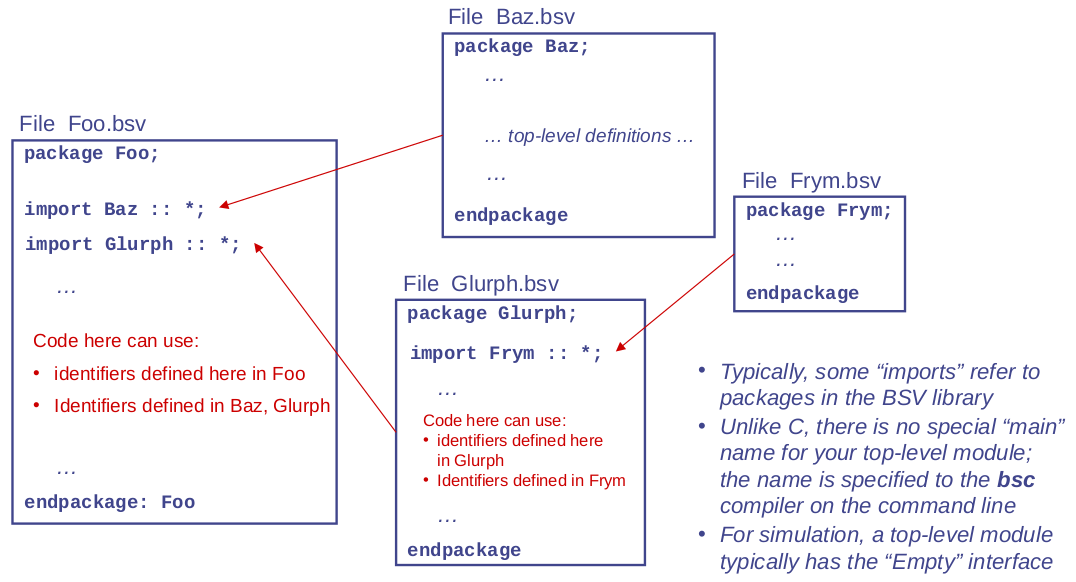
\includegraphics[width=\textwidth]{Figures/fig_Overall_Structure}}
    \caption{%
        \label{fig_OverallStructure}
        Overall structure of a {\BSV} program.
    }
\end{figure}
shows the structure of a sample program.

Figure~\ref{fig_Contents_Package}
\begin{figure}[htbp]
    \centerline{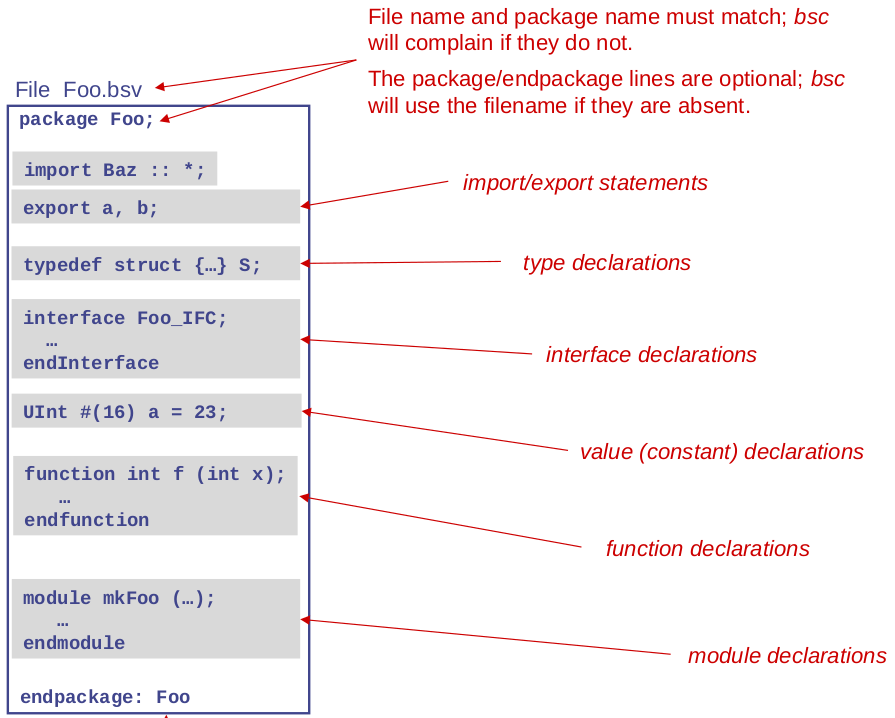
\includegraphics[height=3.5in]{Figures/fig_Contents_Package}}
    \caption{%
        \label{fig_Contents_Package}
        Contents of a {\BSV} package.
    }
\end{figure}
shows the kind of top-level constructs one may find in a {\BSV}
package.  Section~\ref{sec-packages} describes packages, and
Section~\ref{sec-scopes} provides more detail about scopes,
controlling the import and export of names, and resolving name
clashes.

Figure~\ref{fig_Contents_Interface_Decl}
\begin{figure}[htbp]
    \centerline{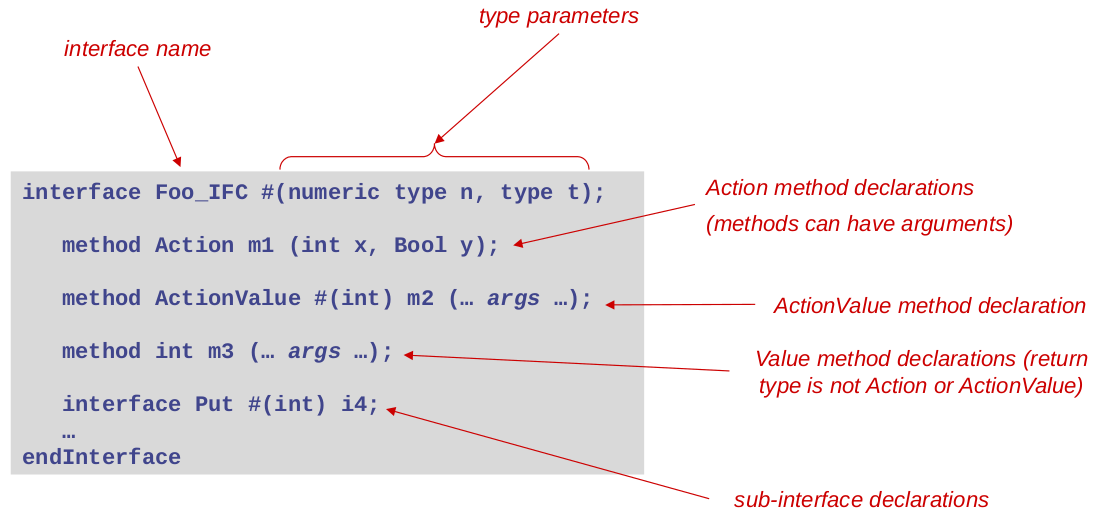
\includegraphics[height=2.5in]{Figures/fig_Contents_Interface_Decl}}
    \caption{%
        \label{fig_Contents_Interface_Decl}
        Contents of a {\BSV} interface declaration.
    }
\end{figure}
shows what goes into an \emph{interface} declaration
(Section~\ref{sec-interface-decl}).  These are \emph{method}
declarations and sub-interface declarations (since interfaces can be
nested hierarchically).

Figure~\ref{fig_Contents_Module_Decl}
\begin{figure}[htbp]
    \centerline{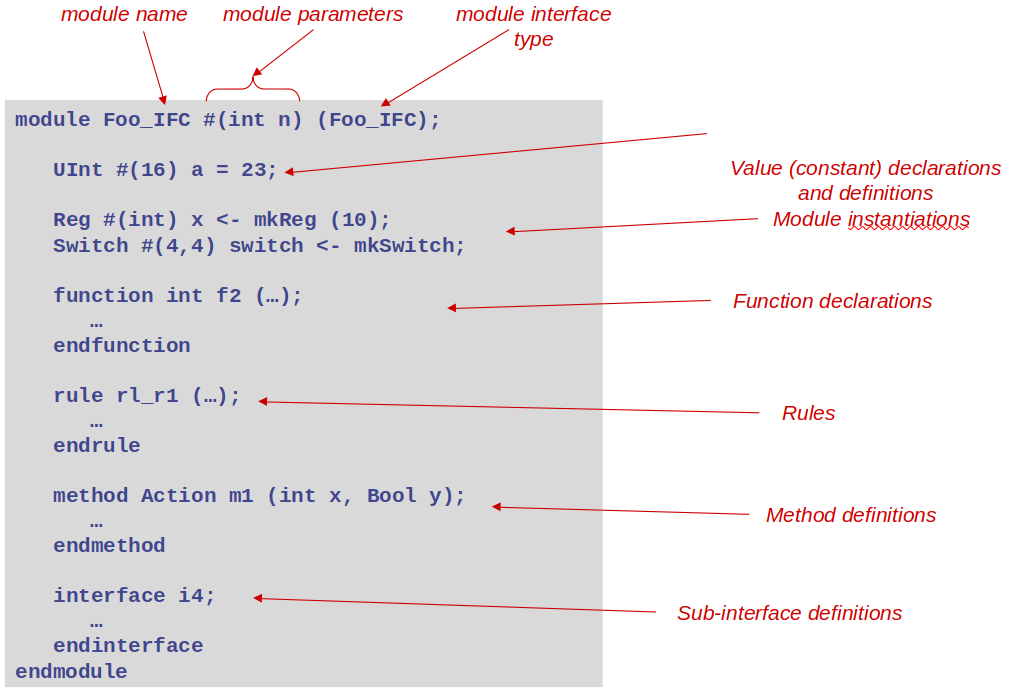
\includegraphics[height=3.5in]{Figures/fig_Contents_Module_Decl}}
    \caption{%
        \label{fig_Contents_Module_Decl}
        Contents of a {\BSV} module declaration.
    }
\end{figure}
shows what goes into a \emph{module} declaration
(Section~\ref{sec-module-decl}).  These are value, function and
(sub)-module declarations and definitions, (sub-)module
instantiations, rules, and definitions of methods and sub-interfaces
implemented (offered) by the module.

Figure~\ref{fig_Contents_Rule}
\begin{figure}[htbp]
    \centerline{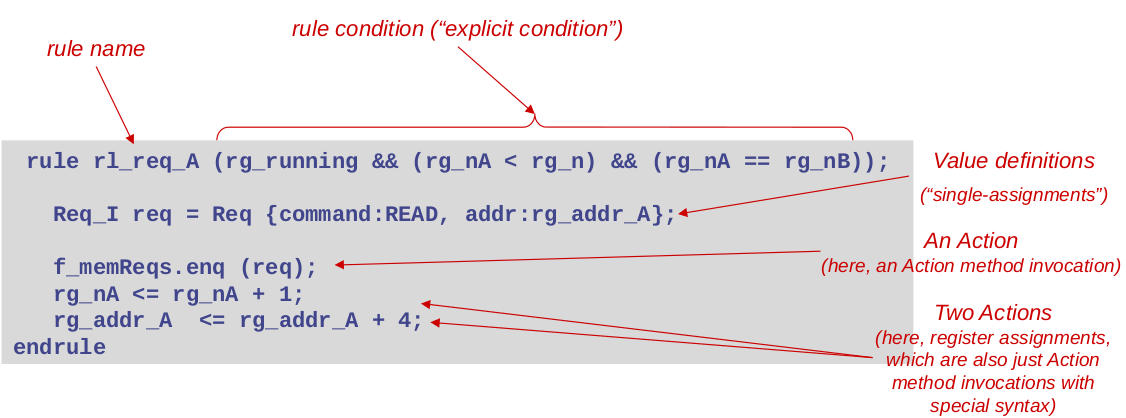
\includegraphics[height=2in]{Figures/fig_Contents_Rule}}
    \caption{%
        \label{fig_Contents_Rule}
        Contents of a {\BSV} rule.
    }
\end{figure}
shows what goes into a \emph{rule}
(Section~\ref{sec-rules-in-modules}).  Each rule has a \emph{rule
  condition} and a \emph{rule body} containing local definitions and
\emph{actions} which perform the semantic actions of the rule.
Actions are typically invocations of methods in other modules.

Figure~\ref{fig_Contents_Method_Def}
\begin{figure}[htbp]
    \centerline{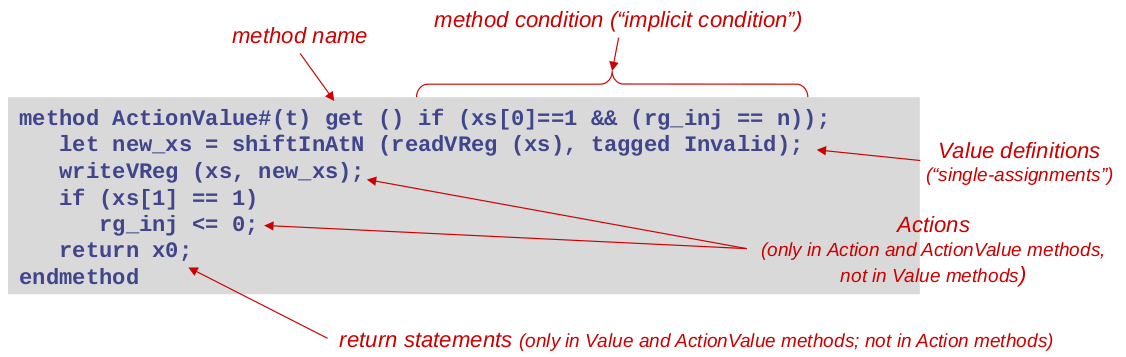
\includegraphics[height=1.75in]{Figures/fig_Contents_Method_Def}}
    \caption{%
        \label{fig_Contents_Method_Def}
        Contents of a {\BSV} method definition (in a module).
    }
\end{figure}
shows what goes into an interface method definition
(Section~\ref{sec-interface-definition}).  These are similar in
structure to rules containing a condition and a body (in fact, a
method definition is semantically a fragment of a rule that invokes
it).

All of the above describe the \emph{textual} structure of a {\BSV}
program.  When compiled to hardware, it undergoes \emph{static
  elaboration}:
\index{static elaboration}
an instance of the top-level module instantiates its
sub-modules, in turn, instantiate their sub-modules, and so on,
recursively, forming a tree structure (a nesting structure).  This
struucture is illustrated in Figure~\ref{fig_Contents_Elaborated}
\begin{figure}[htbp]
    \centerline{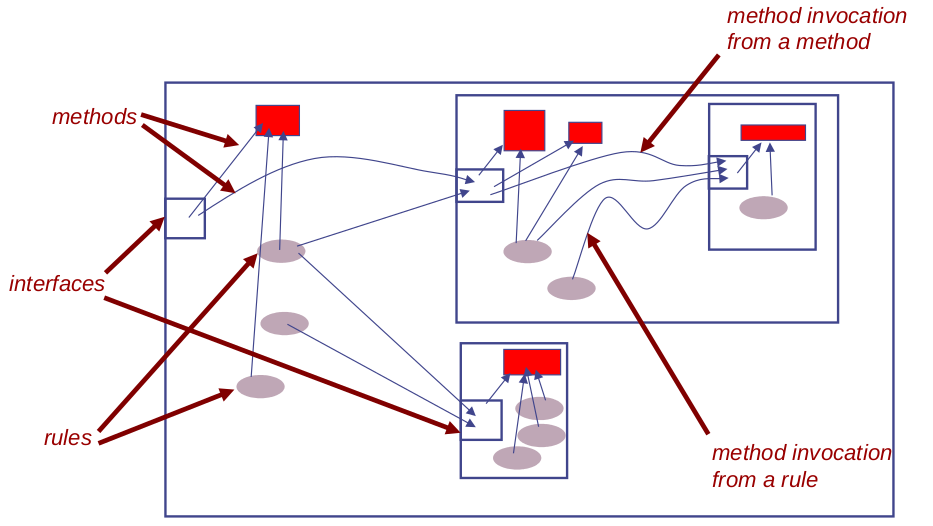
\includegraphics[height=3in]{Figures/fig_Contents_Elaborated}}
    \caption{%
        \label{fig_Contents_Elaborated}
        The (fixed) hardware strucuture of a {\BSV} program after static elaboration.
    }
\end{figure}

% ================================================================

\section{Lexical elements}

{\BSV} has the same basic lexical elements as {\V}.

% ----------------------------------------------------------------

\subsection{Whitespace and comments}

Spaces, tabs, newlines, formfeeds, and carriage returns all constitute
whitespace.  They may be used freely between all lexical tokens.

A \emph{comment} is treated as whitespace (it can only occur between,
and never within, any lexical token).  A one-line comment
\index{comment!one-line}
\index{//@\te{//} (one-line comment)}
starts with \texttt{//} and ends with a newline.  A block comment
\index{comment!block}
\index{/*@\te{/*} (open block comment)}
\index{*/@\te{*/} (close nested comment)}
begins with
\texttt{/*} and ends with \texttt{*/} and may span any number of lines.

Comments do not nest.  In a one-line comment, the character sequences
\texttt{//}, \texttt{/*} and \texttt{*/} have no special significance.  In a
block comment, the character sequences \texttt{//} and \texttt{/*} have no
special significance.

% ----------------------------------------------------------------

\subsection{Identifiers and keywords}

\index{identifiers}
An identifier in {\BSV} consists of any
sequence of letters, digits, dollar signs \texttt{\$} and underscore
characters (\texttt{\_}).
\index{underscore|see{\_}}
\index{_@\$ (character in identifiers)}
\index{_@\te{\_} (character in identifiers)}
Identifiers are case-sensitive: {\tt{glurph}}, {\tt{gluRph}} and
{\tt{Glurph}} are three distinct identifiers.  The first character
cannot be a digit.

{\BSV} currently requires a certain capitalization convention for the
first letter in an identifier.  Identifiers used for package names,
type names, enumeration labels, union members and type classes must
begin with a capital letter.  In the syntax, we use the non-terminal
{\nterm{Identifier}} to refer to these.  Other identifiers (including
names of variables, modules, interfaces, etc.)  must begin with a
lowercase letter and, in the syntax, we use the non-terminal
{\nterm{identifier}} to refer to
\index{identifiers!case sensitivity}
\index{identifier@{\nterm{identifier}} (grammar terminal)}
\index{identifier@{\nterm{Identifier}} (grammar terminal)}
these.

As in {\V}, identifiers whose first character is \term{\$}
\index{identifiers!with \$ as first letter}
are reserved for so-called \emph{system tasks and functions}
(see Section \ref{sec-system-tasks-and-functions}).


If the first character of an instance name is an
underscore, (\te{\_}), the  compiler will not generate this instance
in the Verilog hierarchy name. This
can be useful for removing submodules from the hierarchical naming.


There are a number of \emph{keywords} that are essentially reserved
identifiers, i.e., they cannot be used by the programmer as
identifiers.  Keywords generally do not use uppercase letters (the
only exception is the keyword \texttt{valueOf}).  {\BSV} includes all
keywords in {\SV}.  All keywords are listed in Appendix
\ref{sec-keywords}.

The types \texttt{Action} and \texttt{ActionValue} are special, and cannot
be redefined.

% ----------------------------------------------------------------

\subsection{Integer literals}

\label{sec-integer-literals}

\index{Literals!Integer}
\index{Integer literals}
Integer literals are written with the usual Verilog and C notations:

\gram{intLiteral}{ \term{'0} {\alt} \term{'1}}\\
\gramalt         { \nterm{sizedIntLiteral}}\\
\gramalt         { \nterm{unsizedIntLiteral} }

\gram{sizedIntLiteral}{ \nterm{bitWidth}  \nterm{baseLiteral}}

\gram{unsizedIntLiteral}{ {\opt{\nterm{sign}} \nterm{baseLiteral}}}\\
\gramalt                { {\opt{\nterm{sign}} \nterm{decNum}}}


\gram{baseLiteral} {(\term{'d} {\alt} \term{'D}) \nterm{decDigitsUnderscore}}\\
\gramalt           {(\term{'h} {\alt} \term{'H}) \nterm{hexDigitsUnderscore}}\\
\gramalt           {(\term{'o} {\alt} \term{'O}) \nterm{octDigitsUnderscore}}\\
\gramalt           {(\term{'b} {\alt} \term{'B}) \nterm{binDigitsUnderscore}}\\

\gram{decNum} {\nterm{decDigits} \opt{\nterm{decDigitsUnderscore}}}\\

\gram{bitWidth}{ \nterm{decDigits} }

\gram{sign}{\term{+} {\alt} \term{-}}\\

\gram{decDigits}{\many{\texttt{0}...\texttt{9}}} \\
\gram{decDigitsUnderscore} {\many{\texttt{0}...\texttt{9}, \te{\_}}}\\
\gram{hexDigitsUnderscore}{\many{\texttt{0}...\texttt{9}, \te{a...f},
\te{A...F}, \te{\_}}} \\
\gram{octDigitsUnderscore}{\many{\texttt{0}...\texttt{7}, \te{\_}}}\\
\gram{binDigitsUnderscore}{\many{\texttt{0},\texttt{1}, \te{\_}}}



An integer literal is a sized  integer literal  if a specific
\nterm{bitWidth} is given (e.g., {\tt 8'o255}).  
There is no leading \nterm{sign} (\te{+} or \te{-}) in the syntax for sized integer
literals; instead we provide unary prefix \texttt{+} or \texttt{-}
operators that can be used in front of any integer expression,
including literals (see Section \ref{sec-exprs}).  An optional sign (\te{+} or \te{-})  is 
part of the syntax for unsized literals so that it is possible to construct
negative constants whose negation is not in the range of the type being constructed
(e.g. \texttt{Int\#(4) x = -8;} since \texttt{8} is not a valid \texttt{Int\#(4)}, 
but \texttt{-8} is).  

Examples:
\begin{verbatim}
 125
 -16
 'h48454a
 32'h48454a
 8'o255
 12'b101010
 32'h_FF_FF_FF_FF
\end{verbatim}

% ----------------

\subsubsection{Type conversion of integer literals}

\label{sec-typeconv-integer-literals}

Integer literals can be used to specify values for various integer
types and even for user-defined types. {\BSV} uses its systematic
overloading resolution mechanism to perform these type conversions.
Overloading resolution is described in more detail in Section
{\ref{sec-overloading}}.

An integer literal is a sized literal if a specific \nterm{bitWidth}
is given (e.g., {\tt 8'o255}), in which case the literal is assumed to
have type \texttt{bit~[$w-1$:0]}.  The compiler implicitly applies the
function \texttt{fromSizedInteger}
\index{fromSizedInteger@\te{fromSizedInteger} (\te{SizedLiteral} class
  method)} to the literal to convert it to the type required by the
context.  Thus, sized literals can be used for any type on which the
overloaded function \texttt{fromSizedInteger} is defined, i.e., for
the types \te{Bit}, \te{UInt} and \te{Int}.  The function
\te{fromSizedInteger} is part of the \te{SizedLiteral} typeclass,
described in {\LibRefGuide}.

If the literal is an unsized integer literal (a specific
\nterm{bitWidth} is not given), the literal is assumed to have type
\texttt{Integer}.  The compiler implicitly applies the overloaded
function \texttt{fromInteger} \index{fromInteger@\te{fromInteger}
  (\te{Literal} class method)} to the literal to convert it to the
type required by the context.  Thus, unsized literals can be used for
any type on which the overloaded function \texttt{fromInteger} is
defined.  The function \te{fromInteger} is part of the \te{Literal}
typeclass, described in {\LibRefGuide}.

The literal \texttt{'0} just stands for 0.  The literal \texttt{'1} stands
for a value in which all bits are 1 (the width depends on the
context).

% ----------------------------------------------------------------

\subsection{Real literals}

\label{sec-real-literals}

\index{Literals!Real}
\index{Real literals}
% Support for \texttt{real} ({\VTwoK}) and \texttt{shortreal} ({\SV}) will be
% added to {\BSV} in the future.

Real number literals are written with the usual Verilog notation:

\gram{realLiteral}{\nterm{decNum}{\opt{\term{.}\nterm{decDigitsUnderscore}}} \nterm{exp}
\opt{\nterm{sign}} \nterm{decDigitsUnderscore}}\\
\gramalt{\nterm{decNum}\term{.}\nterm{decDigitsUnderscore}}

\gram{sign}{\term{+} {\alt} \term{-}}

\gram{exp}{\term{e} {\alt} \term{E}}

\gram{decNum} {\nterm{decDigits} \opt{\nterm{decDigitsUnderscore}}}

\gram{decDigits}{\many{\texttt{0}...\texttt{9}}} \\
\gram{decDigitsUnderscore} {\many{\texttt{0}...\texttt{9}, \te{\_}}}\\


There is no leading sign (\te{+} or \te{-}) in the syntax for real
literals.  Instead, we provide the unary prefix \te{+} and \te{-}
operators that can be used in front of any expression, including real
literals (Section \ref{sec-exprs}).

If the real literal contains a decimal point,  there must be  digits following 
the decimal point.  An exponent can start with  either an \te{E} or
an \te{e}, followed by an optional 
sign (\te{+} or \te{-}), followed by digits.  There cannot be an
exponent or a sign without any digits.  Any of the numeric components
may include an underscore, but an underscore cannot be the first digit
of the real literal.

Unlike integer literals, real literals are of limited precision.  They are
represented as IEEE floating point numbers of 64 bit length, as defined by
the IEEE standard.
 
% The \te{Real} type is used for static elaboration only; all values must be
% resolved at compile time.

Examples:
\begin{verbatim}
1.2
0.6
2.4E10                    // exponent can be e or E
5e-3
325.761_452_e-10          // underscores are ignored
9.2e+4
\end{verbatim}


\subsubsection{Type conversion of real literals}

Real literals can be used to specify values for real types.  By
default, real literals are assumed to have the type \te{Real}. {\BSV}
uses its systematic overloading resolution mechanism to perform these
type conversions.  Overloading resolution is described in more detail
in Section {\ref{sec-overloading}}.  There are additional functions
defined for \te{Real} types, provided in the \te{Real} package
described in {\LibRefGuide}.

The function \te{fromReal} (described in {\LibRefGuide}) converts a
value of type \te{Real} into a value of another datatype.  Whenever
you write a real literal in BSV (such as \te{3.14}), there is an
implied \te{fromReal} applied to it, which turns the real into the
specified type.  By defining an instance of \te{RealLiteral} for a
datatype, you can create values of that type from real literals.

The type \te{FixedPoint}, defined in the \te{FixedPoint} package,
defines a type for representing fixed point numbers.  The
\te{FixedPoint} type has an instance of \te{RealLiteral} defined for
it and contains functions for operating on fixed-point real numbers.

% ----------------------------------------------------------------

\subsection{String literals}

\label{sec-string-literals}

\index{Literals!String}
\index{String literals}

String literals are written enclosed in double quotes \texttt{"$\cdots$"} and must
be contained on a single source line.

\gram{stringLiteral}{ \term{"} $\cdots$ string characters $\cdots$ \term{"} }

Special characters may be inserted in string literals with the
following backslash escape sequences:
\begin{tabbing}
 \texttt{{\BSL}n}    \hmmmm \= newline \\
 \texttt{{\BSL}t}           \> tab \\
 \texttt{{\BSL}{\BSL}}      \> backslash \\
 \texttt{{\BSL}"}           \> double quote \\
 \texttt{{\BSL}v}           \> vertical tab \\
 \texttt{{\BSL}f}           \> form feed \\
 \texttt{{\BSL}a}           \> bell \\
 \texttt{{\BSL}$OOO$}       \> exactly 3 octal digits (8-bit character code) \\
 \texttt{{\BSL}x$HH$}       \> exactly 2 hexadecimal digits (8-bit character code)
\end{tabbing}

Example - printing characters using form feed.
\begin{libverbatim}
     module mkPrinter (Empty);
        String display_value;

        display_value = "a\nb\nc";    //prints a
                                      //       b
                                      //       c   repeatedly
        rule every;
           $display(display_value);
        endrule
     endmodule
\end{libverbatim}

% TODO: fixup to the following text after Mieszko has fixed the compiler
% If fewer than three octal digits are used in the octal character code
% escape sequence, they must be followed by a non-octal digit or by the
% end of the string.

% If fewer than two hexadecimal digits are used in the hexadecimal
% character code escape sequence, they must be followed by a
% non-hexadecimal digit or by the end of the string.


\subsubsection{Type conversion of string literals}

String literals are used to specify values for string types.  BSV uses
its systematic overloading resolution mechanism to perform these type
conversions.  Overloading resolution is described in more detail in
Section {\ref{sec-overloading}}.

Whenever you write a string literal in BSV there is an  implicit
\te{fromString} applied to it, which defaults to type \te{String}.  

% ----------------------------------------------------------------

\subsection{Don't-care values}

A lone question mark \texttt{?} is treated as a special don't-care value.
For example, one may return \texttt{?} from an arm of a case statement
that is known to be unreachable.
\index{?@\texttt{?} (don't-care expression)}
\index{don't-care expression|see {?}}

Example - Using \te{?} as a don't-care value
\begin{libverbatim}
     module mkExample (Empty);
        Reg#(Bit#(8)) r <- mkReg(?);     // don't-care is used for the  
        rule every;                      // reset value of the Reg
           $display("value is %h", r);   // the value of r is displayed
        endrule
     endmodule
\end{libverbatim}
% ----------------------------------------------------------------

\subsection{Compiler directives}

\index{compiler directives}

\index{compiler directives}
\index{`@\te{`}|see{compiler directives}}
The following compiler directives permit file inclusion, macro
definition and substitution, and conditional compilation.  They follow
the specifications given in the {\VTwoK} LRM plus the extensions given
in the {\SVThreeOneA} LRM.

In general, these compiler directives can appear anywhere in the
source text.  In particular, they do not need to be on lines by
themselves, and they need not begin in the first column.  Of course,
they should not be inside strings or comments, where the text remains
uninterpreted.

% ----------------

\subsubsection{File inclusion: `include and `line}

\index{include@\te{`include} (compiler directive)}

\gram{compilerDirective}{ \term{`include "}\nterm{filename}\term{"} } \\
\gramalt                { \term{`include <}\nterm{filename}\term{>} } \\
\gramalt                { \term{`include}  \nterm{macroInvocation} }

In an \texttt{`include} directive, the contents of the named file are
inserted in place of this line.  The included files may themselves
contain compiler directives.  Currently there is no difference between
the \te{"..."} and \te{<...>} forms.  A \nterm{macroInvocation} should
expand to one of the other two forms.  The file name may be absolute,
or relative to the current directory.

\gram{compilerDirective}{ \term{`line} \nterm{lineNumber} \term{"}\nterm{filename}\term{"} \nterm{level} } \\
\gram{lineNumber}{ \nterm{decLiteral} } \\
\gram{level}{ \term{0} {\alt} \term{1} {\alt} \term{2} }

\index{line@\te{`line} (compiler directive)}
A \texttt{`line} directive is terminated by a newline, i.e., it cannot
have any other source text after the \nterm{level}.  The compiler
automatically keeps track of the source file name and line number for
every line of source text (including from included source files), so
that error messages can be properly correlated to the source.  This
directive effectively overrides the compiler's internal tracking
mechanism, forcing it to regard the next line onwards as coming from
the given source file and line number.  It is generally not necessary
to use this directive explicitly; it is mainly intended to be
generated by other preprocessors that may themselves need to alter the
source files before passing them through the {\BSV} compiler; this
mechanism allows proper references to the original source.

The \nterm{level} specifier is either 0, 1 or 2:
\begin{itemize}
\item
1 indicates that an include file has just been entered
\item
2 indicates that an include file has just been exited
\item
0 is used in all other cases
\end{itemize}

% ----------------
\label{sec-macrodef}
\subsubsection{Macro definition and substitution: `define and related directives}

\gram{compilerDirective}{ \term{`define} \nterm{macroName}
                              \opt{ \term{(} \nterm{macroFormals} \term{)} }
                              \nterm{macroText} }

\gram{macroName}{ \nterm{identifier} }

\gram{macroFormals}{ \nterm{identifier} \many { \term{,} \nterm{identifier} } }

\index{define@\te{`define} (compiler directive)}
The \texttt{`define} directive is terminated by a bare newline.  A
backslash (\verb'\') just before a newline continues the directive
into the next line.  When the macro text is substituted, each such
continuation backslash-newline is replaced by a newline.

The \nterm{macroName} is an identifier and may be followed by formal
arguments, which are a list of comma-separated identifiers in
parentheses.  For both the macro name and the formals, lower and upper
case are acceptable (but case is distinguished).  The
{\nterm{macroName}} cannot be any of the compiler directives (such as
\texttt{include}, \texttt{define}, ...).

The scope of the formal arguments extends to the end of the
\nterm{macroText}.

The \nterm{macroText} represents almost arbitrary text that is to be
substituted in place of invocations of this macro. The
{\nterm{macroText}} can be empty.

One-line comments (i.e., beginning with \texttt{//}) may appear in the
{\nterm{macroText}}; these are not considered part of the
substitutable text and are removed during substitution.  A one-line
comment that is not on the last line of a \texttt{`define} directive is
terminated by a backslash-newline instead of a newline.

A block comment (\texttt{/*...*/}) is removed during substitution and
replaced by a single space.

The \nterm{macroText} can also contain the following special escape
sequences:
\begin{itemize}

\item
\verb|`"| \hmmm
Indicates that a double-quote (\texttt{"}) should be placed in the
expanded text.

\item
\verb|`\`"| \hmm
Indicates that a backslash and a double-quote (\verb|\"|) should be
placed in the expanded text.

\item
\verb|``| \hmmm
Indicates that there should be no whitespace between the preceding and
following text.  This allows construction of identifiers from the
macro arguments.

\end{itemize}
A minimal amount of lexical analysis of \nterm{macroText} is done to
identify comments, string literals, identifiers representing macro
formals, and macro invocations.  As described earlier, one-line
comments are removed.  The text inside string literals is not
interpreted except for the usual string escape sequences described in
Section {\ref{sec-string-literals}}.

There are two define-macros in the define environment initially;
\texttt{`bluespec} and \texttt{`BLUESPEC}.

Once defined, a macro can be invoked anywhere in the source text
(including within other macro definitions) using the following syntax.

\gram{compilerDirective}{ \nterm{macroInvocation} }

\gram{macroInvocation}{ \term{`}\nterm{macroName}
                              \opt{ \term{(} \nterm{macroActuals} \term{)} } }

\gram{macroActuals}{ \nterm{substText} \many { \term{,} \nterm{substText} } }

\index{macro invocation (compiler directive)}
The \nterm{macroName} must refer to a macro definition available at
expansion time.  The \nterm{macroActuals}, if present, consist of
substitution text \nterm{substText} that is arbitrary text, possibly
spread over multiple lines, excluding commas.  A minimal amount of
parsing of this substitution text is done, so that commas that are not
at the top level are not interpreted as the commas separating
{\nterm{macroActuals}}.  Examples of such ``inner'' uninterpreted
commas are those within strings and within comments.

\gram{compilerDirective}{ \term{`undef} \nterm{macroName} } \\
\gramalt                { \term{`resetall} }

\index{undef@\te{`undef} (compiler directive)}
\index{resetall@\te{`resetall} (compiler directive)}
The \texttt{`undef} directive's effect is that the specified macro (with
or without formal arguments) is no longer defined for the subsequent
source text. Of course, it can be defined again with \texttt{`define} in
the subsequent text.  The \texttt{`resetall} directive has the effect of
undefining all currently defined macros, i.e., there are no macros
defined in the subsequent source text.


% ----------------

\subsubsection{Conditional compilation: `ifdef and related directives}

\gram{compilerDirective}{ \term{`ifdef}  \nterm{macroName} } \\
\gramalt                { \term{`ifndef} \nterm{macroName} } \\
\gramalt                { \term{`elsif} \nterm{macroName} } \\
\gramalt                { \term{`else} } \\
\gramalt                { \term{`endif} }

\index{ifdef@\te{`ifdef} (compiler directive)}
\index{ifndef@\te{`ifndef} (compiler directive)}
\index{elsif@\te{`elsif} (compiler directive)}
\index{else@\te{`else} (compiler directive)}
\index{endif@\te{`endif} (compiler directive)}
These directives are used together in either an \texttt{`ifdef}-{\tt
endif} sequence or an \texttt{ifndef}-\texttt{endif} sequence.  In either
case, the sequence can contain zero or more \texttt{elsif} directives
followed by zero or one \texttt{else} directives.  These sequences can be
nested, i.e., each \texttt{`ifdef} or \texttt{ifndef} introduces a new,
nested sequence until a corresponding \texttt{endif}.

In an \texttt{`ifdef} sequence, if the \nterm{macroName} is currently
defined, the subsequent text is processed until the next corresponding
\texttt{elsif}, \texttt{else} or \texttt{endif}.  All text from that next
corresponding \texttt{elsif} or \texttt{else} is ignored until the {\tt
endif}.

If the \nterm{macroName} is currently not defined, the subsequent text
is ignored until the next corresponding \texttt{`elsif}, \texttt{`else} or
\texttt{`endif}.  If the next corresponding directive is an \texttt{`elsif},
it is treated just as if it were an \texttt{`ifdef} at that point.

If the \texttt{`ifdef} and all its corresponding \texttt{`elsif}s fail (macros
were not defined), and there is an \texttt{`else} present, then the text
between the \texttt{`else} and \texttt{`endif} is processed.

An \texttt{`ifndef} sequence is just like an \texttt{`ifdef} sequence, except
that the sense of the first test is inverted, i.e., its following text
is processes if the \nterm{macroName} is \emph{not} defined, and its
\texttt{`elsif} and \texttt{`else} arms are considered only if the macro
\emph{is} defined.

Example using `ifdef to determine the size of a register:
\begin{verbatim}
     `ifdef USE_16_BITS       
        Reg#(Bit#(16)) a_reg <- mkReg(0);
     `else
        Reg#(Bit#(8)) a_reg <- mkReg(0);
     `endif
\end{verbatim}

% ================================================================

\section{Packages and the outermost structure of a {\BSV} design}

\label{sec-packages}

\index{package}

A {\BSV} program consists of one or more outermost constructs called
packages.  All {\BSV} code is assumed to be inside a package.  Further, the
{\BSV} compiler and other tools assume that there is one package per
file, and they use the package name to derive the file name.  For
example, a package called \texttt{Foo} is assumed to be located in a file
\texttt{Foo.bsv}.

A {\BSV} package is purely a linguistic namespace-management mechanism
and is particularly useful for programming in the large, so that the
author of a package can choose identifiers for the package components
freely without worrying about choices made by authors of other
packages.  Package structure is usually uncorrelated with hardware
structure, which is specified by the module construct.

A package contains a collection of top-level statements that include
specifications of what it imports from other packages, what it exports
to other packages, and its definitions of types, interfaces,
functions, variables, and modules.  {\BSV} tools ensure that when a
package is compiled, all the packages that it imports have already
been compiled.

\index{package@\texttt{package} (keyword)}
\gram{package}{ \term{package} \nterm{packageIde} \term{;}} \\
\grammore{\many{ \nterm{exportDecl} }} \\
\grammore{\many{ \nterm{importDecl} }} \\
\grammore{\many{ \nterm{packageStmt} }} \\
\grammore{\term{endpackage} \opt{\term{:} \nterm{packageIde}}}
\index{endpackage@\texttt{endpackage} (keyword)}

\index{export@\texttt{export} (keyword)}
\gram{exportDecl}{ \term{export} \nterm{exportItem} \many{ \term{,} \nterm{exportItem} } \term{;} } \\
\gram{exportItem}{ \nterm{identifier} \opt{\term{(..)}} } \\
\gramalt         { \nterm{Identifier} \opt{\term{(..)}} } \\
\gramalt         { \nterm{packageIde} \term{::} \term{*} }

\index{import@\texttt{import} (keyword)}
\gram{importDecl}{ \term{import} \nterm{importItem} \many{ \term{,} \nterm{importItem} } \term{;}} \\
\gram{importItem}{ \nterm{packageIde} \term{::} \term{*} }
% \gramalt         { \nterm{packageIde} \term{::} \nterm{identifier} } \\
% \gramalt         { \nterm{packageIde} \term{::} \nterm{Identifier} }

\gram{packageStmt}{ \nterm{moduleDef} } \\
\gramalt          { \nterm{interfaceDecl} } \\
\gramalt          { \nterm{typeDef} } \\
\gramalt          { \nterm{varDecl} {\alt} \nterm{varAssign} } \\
\gramalt          { \nterm{functionDef} } \\
\gramalt          { \nterm{typeclassDef} } \\
\gramalt          { \nterm{typeclassInstanceDef} } \\
\gramalt          { \nterm{externModuleImport} }

\gram{packageIde}{\nterm{Identifier}}

The name of the package is the identifier following the \texttt{package}
keyword.  This name can optionally be repeated after the {\tt
endpackage} keyword (and a colon).  We recommend using an uppercase
first letter in package names.  In fact, the \texttt{package} and {\tt
endpackage} lines are optional: if they are absent, {\BSV} derives the
assumed package name from the filename.

\index{export, identifiers from a package}
\index{identifiers!export from a package}
\index{(..)@\texttt{(..)} (exporting member names)}
An export item can specify an identifier defined elsewhere within the
package,  making the identifier accessible oustside the package.
%The identifier may optionally be followed by \texttt{(..)}.  % The
% identifier then  becomes accessible outside this package.
An export item can also specify 
an identifier from an imported package. In that case, the imported 
identifier is re-exported from this package, so that it is accessible
by importing this package (without requiring the import of its source 
package). It is also possible to re-export all of the identifiers 
from an imported package by using the following syntax: 
\texttt{export packageIde::*}.

 
If there are any export statements in a package, then only 
those items are exported. If there are no export statements, 
by default all identifiers defined in this package (and no identifiers 
from any imported packages) are exported. % To export all identifiers
% defined in a package  and all identifiers from imported packages,
% export the package itself. 

If the exported identifier is the name of a struct (structure) or
union type definition, then the members of that type will be visible
only if \texttt{(..)}  is used.  By omitting the \texttt{(..)} suffix, only
the type, but not its members, are visible outside the package.  This
is a way to define abstract data types, i.e., types whose internal
structure is hidden.  When the exported identifier is not a structure
or union type definition, the \te{(..)} has no effect on the exported
identifier. 

\index{import, identifiers into a package}
\index{identifiers!import into a package}
Each import item specifies a package from which to import identifiers,
i.e., to make them visible locally within this package.  For each
imported package, all identifiers exported from that package are made
locally visible.

Example:
\begin{quote}
\texttt{package Foo;} \\
\texttt{export x;} \\
\texttt{export y;} \\
\hm \\
\texttt{import Bar::*;} \\
%\texttt{import Glurph::z;} \\
\hm \\
{\rm\emph{... top level definition ...}} \\
{\rm\emph{... top level definition ...}} \\
{\rm\emph{... top level definition ...}} \\
\hm \\
\texttt{endpackage: Foo}
\end{quote}

Here, \texttt{Foo} is the name of this package. The identifiers \texttt{x}
and \texttt{y}, which must be defined by the top-level definitions in
this package are names exported from this package.  From package {\tt
Bar} we import all its definitions.    To export all identifiers from
 packages \te{Foo} and \te{Bar}, add the statement: \te{export Foo ::*}
%From package \texttt{Glurph} we
%import just the identifier \texttt{z}.

% ----------------------------------------------------------------

\subsection{Scopes, name clashes and qualified identifiers}

\label{sec-scopes}

\index{identifiers!static scoping}
{\BSV} uses standard static scoping (also known as lexical scoping).
Many constructs introduce new scopes nested inside their surrounding
scopes.  Identifiers can be declared inside nested scopes.  Any use of
an identifier refers to its declaration in the nearest textually
surrounding scope.  Thus, an identifier \texttt{x} declared in a nested
scope ``shadows'', or hides, any declaration of \texttt{x} in surrounding
scopes.  We recommend, however, that the programmer avoids such
shadowing, because it often makes code more difficult to read.

Packages form the the outermost scopes.  Examples of nested scopes
include modules, interfaces, functions, methods, rules, action and
actionvalue blocks, begin-end statements and expressions, bodies of
for and while loops, and seq and par blocks.

\index{identifiers!qualified}
When used in any scope, an identifier must have an unambiguous
meaning.  If there is name clash for an identifier $x$ because it is
defined in the current package and/or it is available from one or more
imported packages, then the ambiguity can be resolved by using a
qualified name of the form $P::x$ to refer to the version of $x$
contained in package $P$.

% ----------------------------------------------------------------

\subsection{Importing the Standard Prelude and Libraries}

\index{Prelude|see{Standard Prelude}}
\index{Standard Prelude}

The Standard Prelude is imported \emph{implicitly} into every {\BSV}
package; there is no explicit \texttt{import} statement.  All other
library packages need an \te{import} statement.

Although not a requirement, as a matter of good style we recommend
against using any of the Standard Prelude names for new definitions in
your programs.  That would require the entity's name to be qualified
with the package name, and may also be confusing to others who read
the code.

% ================================================================


\section{Types}

\label{sec-type}

\index{types}

{\BSV} provides a strong, static type-checking environment; every
variable and every expression in {\BSV} has a {\emph{type}}.
Variables must be assigned values which have compatible types.  Type
checking, which occurs before program elaboration or execution,
ensures that object types are compatible and applied functions are
valid for the context and type.

Data types in \te{\BSV} are case sensitive.  The first character of a
type is almost always uppercase, the only exceptions being the types
\te{int} and \te{bit} for compatibility with Verilog. 

\index{type declaration}

The syntax of types (type expressions) is given below:

\gram{type}{ \nterm{typePrimary} } \\
\gramalt   { \nterm{typePrimary} \term{(} \nterm{type} \many{ \term{,} \nterm{type} } \term{)} } \hfill Function type

\gram{typePrimary}{ \nterm{typeIde} \opt{\term{\#} \term{(} \nterm{type} \many{ \term{,} \nterm{type}} \term{)}} } \\
\gramalt   {\nterm{typeNat}} \\
\gramalt   {\term{bit} \term{[} \nterm{typeNat} \term{:} \nterm{typeNat} \term{]} } \\

\gram{typeIde}{ \nterm{Identifier} } \\
\gram{typeNat}{ \nterm{decDigits} }

The {\LibRefGuide} describes the \te{Prelude} package, which defines
many common datatypes, and the Foundation library packages which
define many more datatypes.  And, users can define new types (Section
\ref{sec-typedefs}).  The following tables list some of the more
commonly used types.

\begin{center}
\begin{tabular}{|p{1 in}|p {3 in}|}
\hline
\multicolumn{2}{|c|}{Common Bit Types Defined in Prelude ({\LibRefGuide})}\\
\multicolumn{2}{|c|}{Bit types are synthesizable}\\
% ----------------
\hline
Type & Description \\
\hline
\hline
% ----------------
\te{Bit\#(n)} & Polymorphic data type containing n bits \\
\hline
% ----------------
\te{UInt\#(n)} & Unsigned fixed-width representation of an integer value of n bits \\
\hline
% ----------------
\te{Int\#(n)} & Signed fixed-width representation of an integer value of n bit \\
\hline
% ----------------
\te{Bool} & Type which can have two values, \te{True} or \te{False} \\
\hline
% ----------------
Maybe
& Used to tag values as \te{Valid} or \te{Invalid}, where valid values contain data \\
\hline
% ----------------
Tuples
& Predefined structures which group a small number of values together \\
\hline
% ----------------
\end{tabular}
\end{center}

\begin{center}
\begin{tabular}{|p{1 in}|p {3 in}|}
\hline
\multicolumn{2}{|c|}{Common Non-Bit Types Defined in Prelude (\LibRefGuide)}\\
\hline
% ----------------
Type & Description \\
\hline
\hline
% ----------------
Integer
& Non-synthesizable data type used for integer values and functions \\
\hline
% ----------------
Real
& Non-synthesizable data type which can represent numbers with a fractional component \\
\hline
% ----------------
String, Char
& Data type representing string literals \\
\hline
% ----------------
Fmt
& Representation of arguments to the \te{\$display} family of tasks \\
\hline
% ----------------
\end{tabular}
\end{center}

\begin{center}
\begin{tabular}{|p{1 in}|p {3 in}|}
\hline
\multicolumn{2}{|c|}{Common Interface Types Defined in Prelude and Foundation
Library Packages}\\
\hline
% ----------------
Type & Description \\
\hline
\hline
% ----------------
\te{Reg} & Register interface \\
\hline
% ----------------
\te{FIFO} & FIFO interfaces \\
\hline
% ----------------
\te{Clock} & Abstract type with a oscillator and a gate \\
\hline
% ----------------
\te{Reset} & Abstract type for a reset \\
\hline
% ----------------
\te{Inout} & Type used to pass Verilog inouts through a BSV module \\
\hline
% ----------------
\end{tabular}
\end{center}

\begin{center}
\begin{tabular}{|p{1 in}|p {3 in}|}
\hline
\multicolumn{2}{|c|}{Types Used by the Compiler}\\
\hline
% ----------------
Type & Description \\
\hline
\hline
% ----------------
\te{Action} & An expression intended to act on the state of the circuit \\
\hline
% ----------------
\te{ActionValue} & An expression intended  to act on the state of the circuit \\
\hline
% ----------------
\te{Rules} & Used to represent one or more rules as a first class type \\
\hline
% ----------------
\te{Module} & A hardware module containing sub-modules, rules and an interface \\
\hline
% ----------------
\end{tabular}
\end{center}


Examples of simple types:
\begin{verbatim}
 Integer                 // Unbounded signed integers, for static elaboration only
 int                     // 32-bit signed integers
 Bool
 String
 Action
\end{verbatim}

\index{types!parameterized}
Type expressions of the form \texttt{$X$\#($t_1$,$\cdots$,$t_N$)} are called
\emph{parameterized}
types.  $X$ is called a \emph{type constructor} and the types
$t_1$,$\cdots$,$t_N$ are the parameters of $X$.
Examples:
\begin{verbatim}
 Tuple2#(int,Bool)           // pair of items, an int and a Bool
 Tuple3#(int,Bool,String)    // triple of items, an int, a Bool and a String
 List#(Bool)                 // list containing booleans
 List#(List#(Bool))          // list containing lists of booleans
 RegFile#(Integer, String)   // a register file (array) indexed by integers, containing strings
\end{verbatim}

\index{size types}
Type parameters can be natural numbers (also known as \emph{numeric} types).  These
usually indicate some aspect of the size of the type, such as a
bit-width or a table capacity.
Examples:
\begin{verbatim}
 Bit#(16)             // 16-bit wide bit-vector (16 is a numeric type)
 bit [15:0]           // synonym for Bit#(16)
 UInt#(32)            // unsigned integers, 32 bits wide
 Int#(29)             // signed integers, 29 bits wide
 Vector#(16,Int#(29)  // Vector of size 16 containing Int#(29)'s
\end{verbatim}
Currently the second index $n$ in a \texttt{bit[$m$:$n$]} type must be 0.
The type \texttt{bit[$m$:0]} represents the type of bit vectors, with
bits indexed from $m$ (msb/left) down through 0 (lsb/right), for $m
\ge 0$.

\index{string types}
Type parameters can also be strings (known as \emph{string} types).
These are not common, but are quite useful in the generics library,
described in the \LibRefGuide.
Examples:
\begin{verbatim}
 MetaData#("Prelude","Maybe",PrimUnit,2)
 MetaConsNamed#("Valid",1,1)
\end{verbatim}

% ----------------------------------------------------------------

\subsection{Polymorphism}

\label{sec-polymorphism-brief}

\index{polymorphism}
A type can be {\emph{polymorphic}}.
\index{types!polymorphic}
This is indicated by using type variables as parameters.
\index{type variables}
Examples:
\begin{verbatim}
 List#(a)                 // lists containing items of some type a
 List#(List#(b))          // lists containing lists of items of some type b
 RegFile#(i, List#(x))    // arrays indexed by some type i, containing
                          //        lists that contain items of some type x
\end{verbatim}
The type variables represent unknown (but specific) types.  In other
words, \texttt{List\#(a)} represents the type of a list containing items
all of which have some type \texttt{a}.  It does not mean that different
elements of a list can have different types.

% ----------------------------------------------------------------

\subsection{Provisos (brief intro)}

\label{sec-provisos-brief}

\index{provisos!brief description}

Provisos are described in detail in Section \ref{sec-provisos}, and
the general facility of type classes (overloading groups), of which
provisos form a part, is described in Section \ref{sec-overloading}.
Here we provide a brief description, which is adequate for most uses
and for continuity in a serial reading of this manual.

A proviso is a static condition attached to certain constructs, to
impose certain restrictions on the types involved in the
construct. The restrictions are of two kinds:
\begin{itemize}

\item
Require instance of a type class (overloading group): this kind of
proviso states that certain types must be instances of certain type
classes, i.e., that certain overloaded functions are defined on this
type.

\item
Require size relationships: this kind of proviso expresses certain
constraints between the sizes of certain types.

\end{itemize}
The most common overloading provisos are:
\index{Bits@\te{Bits} (type class)}                \index{type classes!\te{Bits}}
\index{Eq@\te{Eq} (type class)}                    \index{type classes!\te{Eq}}
\index{Literal@\te{Literal} (type class)}          \index{type classes!\te{Literal}}
\index{Ord@\te{Ord} (type class)}                  \index{type classes!\te{Ord}}
\index{Bounded@\te{Bounded} (type class)}          \index{type classes!\te{Bounded}}
\index{Bitwise@\te{Bitwise} (type class)}          \index{type classes!\te{Bitwise}}
\index{BitReduction@\te{BitReduction} (type class)}\index{type classes!\te{BitReduction}}
\index{BitExtend@\te{BitExtend} (type class)}      \index{type classes!\te{BitExtend}}
\index{Arith@\te{Arith} (type class)}              \index{type classes!\te{Arith}}
\begin{verbatim}
 Bits#(t,n)     // Type class (overloading group) Bits
                // Meaning: overloaded operators pack/unpack are defined
                //     on type t to convert to/from Bit#(n)

 Eq#(t)         // Type class (overloading group) Eq
                // Meaning: overloaded operators == and != are defined on type t

 Literal#(t)    // Type class (overloading group) Literal
                // Meaning: Overloaded function fromInteger() defined on type t
                //     to convert an integer literal to type t. Also overloaded 
                //     function inLiteralRange to determine if an Integer 
                //     is in the range of the target type t.       

 Ord#(t)        // Type class (overloading group) Ord
                // Meaning: Overloaded order-comparison operators <, <=,
                //     > and >= are defined on type t

 Bounded#(t)    // Type class (overloading group) Bounded
                // Meaning: Overloaded identifiers minBound and maxBound
                //     are defined for type t

 Bitwise#(t)    // Type class (overloading group) Bitwise
                // Meaning: Overloaded operators &, |, ^, ~^, ^~, ~, << and >>
                //     and overloaded function invert are defined on type t

 BitReduction#(t)// Type class (overloading group) BitReduction
                // Meaning: Overloaded prefix operators &, |, ^,
                //     ~&, ~|, ~^, and ^~ are defined on type t

 BitExtend#(t)  // Type class (overloading group) BitExtend
                // Meaning: Overloaded functions extend, zeroExtend, signExtend
                //     and truncate are defined on type t

 Arith#(t)      // Type class (overloading group) Arith
                // Meaning: Overloaded operators +, -, and *, and overloaded
                //     prefix operator - (same as function negate), and
                //     overloaded function negate are defined on type t
\end{verbatim}

\index{size types!type classes for constraints}
\index{Add@\te{Add} (type provisos)}    \index{type classes!\te{Add}}
\index{Max@\te{Max} (type provisos)}    \index{type classes!\te{Max}}
\index{Log@\te{Log} (type provisos)}    \index{type classes!\te{Log}}
\index{Mul@\te{Mul} (type provisos)}    \index{type classes!\te{Mul}}
\index{Div@\te{Div} (type provisos)}    \index{type classes!\te{Div}}

The size relationship provisos are:
\begin{verbatim}
 Add#(n1,n2,n3)    // Meaning: assert n1 + n2 = n3

 Mul#(n1,n2,n3)    // Meaning: assert n1 * n2 = n3

 Div#(n1,n2,n3)    // Meaning: assert ceiling n1 / n2 = n3
   
 Max#(n1,n2,n3)    // Meaning: assert max(n1,n2) = n3

 Log#(n1,n2)       // Meaning: assert ceiling(log(n1)) = n2
                   // The logarithm is base 2
\end{verbatim}
Example:
\begin{verbatim}
module mkExample (ProvideCurrent#(a))
   provisos(Bits#(a, sa), Arith#(a));

   Reg#(a) value_reg <- mkReg(?); // requires that type "a" be in the Bits typeclass.
   rule every;
      value_reg <= value_reg + 1; // requires that type "a" be in the Arith typeclass.
   endrule
\end{verbatim}
Example:
\begin{verbatim}
 function Bit#(m) pad0101 (Bit#(n) x)
    provisos (Add#(n,4,m));   // m is 4 bits longer than n
    pad0101 = { x, 0b0101 };
 endfunction: pad0101
\end{verbatim}
This defines a function \texttt{pad0101} that takes a bit vector \texttt{x}
and pads it to the right with the four bits ``0101'' using the standard
bit-concatenation notation.  The types and proviso express the idea
that the function takes a bit vector of length $n$ and returns a bit
vector of length $m$, where $n+4=m$.  These provisos permit the {\BSV}
compiler to statically verify that entities (values, variables,
registers, memories, FIFOs, and so on) have the correct bit-width.

% ----------------

\subsubsection{The pseudo-function \te{valueof} (or \te{valueOf})}

\label{sec-valueof}

To get the value that corresponds to a size type, there is a special
pseudo-function, \texttt{valueof},
\index{valueOf@\texttt{valueOf} (pseudo-function of size types)}
that takes a size type and gives the corresponding \texttt{Integer}
value.  The pseudo-function is also sometimes written as
\texttt{valueOf}; both are considered correct.

\gram{exprPrimary}{ \term{valueof} \term{(} \nterm{type} \term{)}} \\
\gramalt { \term{valueOf} \term{(} \nterm{type} \term{)}}
                 
In other words, it converts from a numeric type expression into an
ordinary value.  These mechanisms can be used to do arithmetic to
derive dependent sizes. Example:
\begin{verbatim}
 function ... foo (Vector#(n,int) xs) provisos (Log#(n,k));
    Integer maxindex = valueof(n) - 1;
    Int#(k) index;
    index = fromInteger(maxindex);
    ...
 endfunction
\end{verbatim}
This function takes a vector of length \texttt{n} as an argument.  The
proviso fixes \texttt{k} to be the (ceiling of the) logarithm of \texttt{n}.
The variable \texttt{index} has bit-width \texttt{k}, which will be adequate
to hold an index into the list.  The variable is initialized to the
maximum index.

Note that the function \texttt{foo} may be invoked in multiple contexts,
each with a different vector length.  The compiler will statically
verify that each use is correct (e.g., the index has the correct
width).

The pseudo-function \texttt{valueof}, which converts a numeric type to a
value, should not be confused with the pseudo-function \texttt{SizeOf},
described in Section {\ref{sec-sizeof}}, which converts a type to a
numeric type.

\subsubsection{The pseudo-function \te{stringof} (or \te{stringOf})}

A function \texttt{stringof} (or \texttt{stringOf})
\index{stringOf@\texttt{stringOf} (pseudo-function of string types)}
similar to \te{valueof}
exists to convert a string type to a string value.
Example:
\begin{verbatim}
 instance CShow'#(Meta#(MetaConsNamed#(name, idx, nfields), a))
  provisos (CShowSummand#(a));
    function cshow'(tagged Meta {x});
      return $format(stringOf(name), " {", cshowSummandNamed(x), "}");
    endfunction
 endinstance
\end{verbatim}

% ----------------------------------------------------------------

\subsection{A brief introduction to \texttt{deriving} clauses}

\label{sec-deriving-brief}

\index{deriving@\texttt{deriving}!brief description}

The \texttt{deriving} clause is a part of the general facility of type
classes (overloading groups), which is described in detail in Section
\ref{sec-overloading}.
Here we provide a brief description, which is adequate for most uses
and for continuity in a serial reading of this manual.

It is possible to attach a \texttt{deriving} clause to a type definition
(Section \ref{sec-typedefs}), thereby directing the compiler to define
automatically certain overloaded functions for that type.  The most
common forms of these clauses are:
\begin{verbatim}
 deriving(Eq)       // Meaning: automatically define == and !=
                    // for equality and inequality comparisons

 deriving(Bits)     // Meaning: automatically define pack and unpack
                    // for converting to/from bits

 deriving(FShow)    // Meaning:  automatically define fshow to convert 
                    // to a Fmt representation for $display functions

 deriving(Bounded)  // Meaning: automatically define minBound and maxBound
\end{verbatim}

Example:
\begin{verbatim}
     typedef enum {LOW, NORMAL, URGENT} Severity deriving(Eq, Bits);
     // == and != are defined for variables of type Severity
     // pack and unpack are defined for variables of type Severity 

     module mkSeverityProcessor (SeverityProcessor);
        method Action process(Severity value);
           // value is a variable of type Severity
           if (value == URGENT) $display("WARNING: Urgent severity encountered.");
           // Since value is of the type Severity, == is defined
        endmethod
     endmodule
\end{verbatim}
% ================================================================

\section{Modules and interfaces, and their instances}

\label{sec-modules-interfaces}
\index{modules!definition of}
\index{interfaces!definition of}

Modules and interfaces form the heart of {\BSV}.  Modules and
interfaces turn into actual hardware.  An interface for a module $m$
mediates between $m$ and other, external modules that use the
facilities of $m$.  We often refer to these other modules as
\emph{clients} of $m$.

In {\SV} and {\BSV} we separate the declaration of an interface from
module definitions.  There was no such separation in {\VOrig} and
{\VTwoK}, where a module's interface was represented by its port list,
which was part of the module definition itself.  By separating the
interface declaration, we can express the idea of a common interface
that may be offered by several modules, without having to repeat that
declaration in each of the implementation modules.

As in {\V} and {\SV}, it is important to distinguish between a module
\emph{definition} and a module \emph{instantiation}.  A module
definition can be regarded as specifying a scheme that can be
instantiated multiple times.  For example, we may have a single module
definition for a FIFO, and a particular design may instantiate it
multiple times for all the FIFOs it contains.

Similarly, we also distinguish interface declarations and instances,
i.e., a design will contain interface declarations, and each of these
may have multiple instances.  For example an interface declaration $I$
may have one instance $i_1$ for communication between module instances
$a_1$ and $b_1$, and another instance $i_2$ for communication between
module instances $a_2$ and $b_2$.

Module instances form a pure hierarchy.  Inside a module definition
$mkM$, one can specify instantiations of other modules.  When $mkM$ is
used to instantiate a module $m$, it creates the specified inner
module instances.  Thus, every module instance other than the top of
the hierarchy unambiguously has a single parent module instance.  We
refer to the top of the hierarchy as the root module.  Every module
instance has a unique set, possibly empty, of child module instances.
If there are no children, we refer to it as a leaf module.

A module consists of three things: state, rules that operate on that
state, and the module's interface to the outside world (surrounding
hierarchy).  The state conceptually consists of all state in the
subhierarchy headed by this module; ultimately, it consists of all
the lower leaf module instances (see next section on state and module
instantiation).  Rules are the fundamental means to express behavior
in {\BSV} (instead of the \texttt{always} blocks used in traditional
{\V}).  In {\BSV}, an interface consists of \emph{methods} that
encapsulate the possible transactions that clients can perform, i.e.,
the micro-protocols with which clients interact with the module.  When
compiled into RTL, an interface becomes a collection of wires.


% ----------------------------------------------------------------

\subsection{Explicit state via module instantiation, not variables}

In {\V} and {\SV} RTL, one simply declares variables, and a synthesis
tool ``infers'' how these variables actually map into state elements
in hardware using, for example, their lifetimes relative to events.  A
variable may map into a bus, a latch, a flip-flop, or even nothing at
all.  This ambiguity is acknowledged in the {\VTwoK} and {\SV}
LRMs.\footnote{In the {\VTwoK} LRM, Section 3.2.2, Variable
declarations, says: ``A \emph{variable} is an abstraction of a data
storage element.$\cdots$NOTE In previous versions of the Verilog
standard, the term \emph{register} was used to encompass both the {\bf
reg}, {\bf integer}, {\bf time}, {\bf real} and {\bf realtime} types;
but that term is no longer used as a Verilog data type.''

In the {\SV} LRM, Section 5.1 says: ``Since the keyword {\bf\tt reg}
no longer describes the user's intent in many
cases,$\cdots$Verilog-2001 has already deprecated the use of the term
\emph{register} in favor of \emph{variable}.''}

{\BSV} removes this ambiguity and places control over state
instantiation explicitly in the hands of the designer.  From the
smallest state elements (such as registers) to the largest (such as
memories), all state instances are specified explicitly using module
instantiation.

Conversely, an ordinary declared variable in {\BSV} \emph{never}
implies state, i.e., it never holds a value over time.  Ordinary
declared variables are always just convenient names for intermediate
values in a computation.  Ordinary declared variables include
variables declared in blocks, formal parameters, pattern variables,
loop iterators, and so on.  Another way to think about this is that
ordinary variables play a role only in static elaboration, not in the
dynamic semantics. This is one of the aspects of {\BSV} style that
may initially appear unusual to the {\V} or {\SV} programmer.

Example:
\begin{verbatim}
     module mkExample (Empty);
        // Hardware registers are created here
        Reg#(Bit#(8)) value_reg <- mkReg(0);

        FIFO#(Bit#(8)) fifo <- mkFIFO;

        rule pop;
           let value = fifo.first();  // value is a ordinary declared variable
                                      // no state is implied or created
           value_reg <= fifo.first(); // value_reg is state variable
           fifo.deq();
         endrule
     endmodule
\end{verbatim}

% ----------------------------------------------------------------

\subsection{Interface declaration}

\label{sec-interface-decl}

\index{interfaces} In {\BSV} an interface contains members that
are called \emph{methods}
\index{methods!of an interface}
(an interface may also contain subinterfaces, which are described in
Section \ref{sec-subinterfaces}).  To first order, a method can be
regarded exactly like a function, i.e., it is a procedure that takes
zero or more arguments and returns a result.  Thus, method
declarations inside interface declarations look just like function
prototypes, the only difference being the use of the keyword {\tt
method} instead of the keyword \texttt{function}.  Each method represents
one kind of transaction between a module and its clients.  When
translated into RTL, each method becomes a bundle of wires.

The fundamental difference between a method and a function is that a
method also carries with it a so-called implicit condition.  These
will be described later along with method definitions and rules.

An interface declaration also looks similar to a struct declaration.
One can think of an interface declaration as declaring a new type
similar to a struct type (Section \ref{sec-typedefs}), where the members all happen to be method
prototypes.  A method prototype is essentially the header of a method
definition (Section \ref{sec-interface-definition}). 

\index{interface@\texttt{interface} (keyword)!in interface declarations}
%\gram{interfaceDecl} {\opt{ \nterm{interfaceAttribute} }  }  \\
\gram{interfaceDecl} {\opt{ \nterm{attributeInstances} }  }  \\
\grammore           { \term{interface} \nterm{typeDefType} \term{;} } \\
\grammore           { \hmm \many{ \nterm{interfaceMemberDecl} } } \\
\grammore           { \term{endinterface} \opt{ \term{:} \nterm{typeIde} } }

%\gram{typeDefType}{\nterm{typeIde} \opt{\term{\#} \term{(}
%\opt{\term{numeric}}  \term{type} \nterm{typeIde} \many{ \term{,} \opt{\term{numeric}} \term{type} \nterm{typeIde}} \term{)}} }

\gram{typeDefType} {\nterm{typeIde} \opt{ \nterm{typeFormals}}

\gram{typeFormals}{\term{\#} \term{(} \nterm{typeFormal} \many{ \term{,} \nterm{typeFormal}}\term{)} }}

\gram{typeFormal}{\opt{\term{numeric} {\alt} \term{string}} \term{type} \nterm{typeIde}}

\gram{interfaceMemberDecl}{ \nterm{methodProto} {\alt} \nterm{subinterfaceDecl} }

%\gram{methodProto}{ \opt{ \nterm{interfaceAttribute} } }\\
\gram{methodProto}{ \opt{ \nterm{attributeInstances} } }\\
\grammore         { \term{method} \nterm{type} \nterm{identifier}
                    \term{(}
                          \opt { \nterm{methodProtoFormals} }
                          \term{)} \term{;}}
%you can put a proviso on a methodProto, but it is a highly advanced
%and non-HW concept. 
%                          \opt{ \nterm{provisos} }


\gram{methodProtoFormals}{ \nterm{methodProtoFormal} \many{ \term{,} \nterm{methodProtoFormal}} }

%\gram{methodProtoFormal}{ \opt{ \nterm{interfaceAttribute} } \nterm{type} \nterm{identifier} }
\gram{methodProtoFormal}{ \opt{ \nterm{attributeInstances} } \nterm{type} \nterm{identifier} }

Example: a stack of integers:
\begin{verbatim}
 interface IntStack;
     method  Action  push  (int x);
     method  Action  pop;
     method  int     top;
 endinterface: IntStack
\end{verbatim}
This describes an interface to a circuit that implements a stack
(LIFO) of integers.  The \texttt{push} method takes an \texttt{int}
argument, the item to be pushed onto the stack.  Its output type is
\texttt{Action}, namely it returns an \emph{enable} wire which, when
asserted, will carry out the pushing action.\footnote{
The type \texttt{Action} is discussed in more detail in Section
{\ref{sec-actions}}.}
The \texttt{pop} method
takes no arguments, and simply returns an enable wire which, when
asserted, will discard the element from the top of the stack.  The
\texttt{top} method takes no arguments, and returns a value of type {\tt
int}, i.e., the element at the top of the stack.

What if the stack is empty?  In that state, it should be illegal to
use the \texttt{pop} and \texttt{top} methods.  This is exactly where the
difference between methods and functions arises.  Each method has an
implicit \emph{ready} wire, which governs when it is legal to use it,
and these wires for the \texttt{pop} and \texttt{top} methods will
presumably be de-asserted if the stack is empty.  Exactly how this is
accomplished is an internal detail of the module, and is therefore not
visible as part of the interface declaration.  (We can similarly
discuss the case where the stack has a fixed, finite depth; in this
situation, it should be illegal to use the \texttt{push} method when
the stack is full.)

One of the major advantages of {\BSV} is that the compiler
automatically generates all the control circuitry needed to ensure
that a method (transaction) is only used when it is legal to use it.

Interface types can be polymorphic, i.e., parameterized by other
types.  For example, the following declaration describes an interface
for a stack containing an arbitrary but fixed type:
\begin{verbatim}
 interface Stack#(type a);
     method  Action  push  (a x);
     method  Action  pop;
     method  a       top;
 endinterface: Stack
\end{verbatim}
We have replaced the previous specific type \texttt{int} with a type
variable \texttt{a}.  By ``arbitrary but fixed'' we mean that a
particular stack will specify a particular type for \texttt{a}, and all
items in that stack will have that type.  It does not mean that a
particular stack can contain items of different types.

For example, using this more general definition, we can also define
the \texttt{IntStack} type as follows:
\begin{verbatim}
 typedef  Stack#(int)  IntStack;
\end{verbatim}
i.e., we simply specialize the more general type with the particular
type \texttt{int}.  All items in a stack of this type will have the {\tt
int} type.

Usually there is information within the interface declaration which
indicates whether a polymorphic interface type is numeric or
nonnumeric.  The optional \te{numeric} is required before the type when the
interface type is polymorphic and must be numeric but there is no
information in the interface declaration which would indicate that the
type is numeric.

For example, in the following polymorphic interface, \te{count\_size}
must be numeric because it is defined as a parameter to \te{Bit\#()}.
\begin{verbatim}
interface Counter#(type count_size);
   method Action increment();
   method Bit#(count_size) read();
endinterface
\end{verbatim}
From this use, it can be deduced that
\te{Counter's} parameter \te{count\_size} must be numeric.  However, sometimes
you might want to encode a size in an interface type which isn't
visible in the methods, but is used by the module implementing the
interface.   For instance:
\begin{verbatim}
interface SizedBuffer#(numeric type buffer_size, type element_type);
   method Action enq(element_type e);
   method ActionValue#(element_type) deq();
endinterface
\end{verbatim}
In this interface, the depth of the buffer is encoded in the type.
For instance, \te{SizedBuffer\#(8, Bool)} would be a buffer of depth 8 with
elements of type \te{Bool}.  The depth is not visible in the interface, but
is used by the module to know how much storage to instantiate.

Because the parameter is not mentioned anywhere else in the interface,
there is no information to determine whether the parameter is a
numeric type or a non-numeric type.  In this situation, the default is
to assume that the parameter is non-numeric.  The user can override
this default by specifying \te{numeric} in the interface declaration. 

The Standard Prelude defines a standard interface called
\te{Empty}\index{Empty@\te{Empty} (interface)} 
which contains no methods, i.e., its definition is: 
\begin{verbatim}
  interface Empty;
  endinterface
\end{verbatim}

This is often used for top-level modules that integrate a testbench
and a design-under-test, and for modules like \texttt{mkConnection}
(see \LibRefGuide) that just take interface arguments and do not
themselves offer any interesting interface.

% ----------------

\subsubsection{Subinterfaces}

\label{sec-subinterfaces}

\index{subinterfaces!declaration of}

Note: this is an advanced topic that may be skipped on first reading.

Interfaces can also be declared hierarchically, using subinterfaces.

%\gram{subinterfaceDecl}{ \opt{ \nterm{interfaceAttribute} } }\\
\gram{subinterfaceDecl}{ \opt{ \nterm{attributeInstances} } }\\
\grammore               { \term{interface} \nterm{typeDefType}\term{;} }

where \nterm{typeDefType} is another interface type available in the current
scope.  Example:
\begin{verbatim}
 interface ILookup;
     interface  Server#( RequestType, ResponseType )  mif;
     interface  RAMclient#( AddrType, DataType )      ram;
     method     Bool  initialized;
 endinterface: ILookup
\end{verbatim}

This declares an interface \texttt{ILookup} module that consists of
three members: a \texttt{Server} subinterface called \texttt{mif}, a
{\tt RAMClient} subinterface called \texttt{ram}, and a boolean method
called \texttt{initialized} (the \texttt{Server} and
\texttt{RAMClient} interface types are defined in \LibRefGuide).
Methods of subinterfaces are accessed using dot notation to select the
desired component, e.g.,

\begin{verbatim}
    ilookup.mif.request.put(...);
\end{verbatim}

Since \texttt{Clock} and \texttt{Reset} are both interface types, they
can be used in interface declarations.  Example:
\begin{verbatim}
 interface ClockTickIfc ;
    method Action tick() ;
    interface Clock  new_clk ;
 endinterface
\end{verbatim}

% ----------------------------------------------------------------

\subsection{Module definition}

\label{sec-module-decl}
\index{module!definition of}

A module definition begins with a module header containing the {\tt
module} keyword, the module name, parameters, arguments, interface type and
provisos.  The header is followed by zero or more module statements.
Finally we have the closing \texttt{endmodule} keyword, optionally
labelled again with the module name.
\index{modules!module@\texttt{module} (keyword)}

\gram{moduleDef} {\opt{\nterm{attributeInstances}}} \\
\grammore       {\nterm{moduleProto}}\\
\grammore       { \hmm \many{ \nterm{moduleStmt} } } \\
\grammore       { \term{endmodule} \opt{ \term{:}  \nterm{identifier} } }

\gram{moduleProto}{\term{module} \opt{\term{[} \nterm{type} \term{]}} {\nterm{identifier}} } \\
\grammore       { \opt{\nterm{moduleFormalParams}} \term{(}
\opt{\nterm{moduleFormalArgs}} \term{)} \opt{\nterm{provisos}}\term{;}}


\gram{moduleFormalParams}{\term{\#} \term{(}\nterm{moduleFormalParam}
\many{\term{,} \nterm{moduleFormalParam}}\term{)} }

\gram{moduleFormalParam}{\opt{\nterm{attributeInstances}} \opt{\term{parameter}} \nterm{type} \nterm{identifier} }

\gram{moduleFormalArgs} \opt{\nterm{attributeInstances}} \nterm{type} \\
\gramalt{\opt{\nterm{attributeInstances}} \nterm{type} \nterm{identifier} }\\
\grammore {\many{\term{,} 
 \opt{\nterm{attributeInstances}} \nterm{type} \nterm{identifier}}}

As a stylistic convention, many {\BSV} examples use module names like
\texttt{mkFoo}, i.e., beginning with the letters \texttt{mk}, suggesting the
word \emph{make}.  This serves as a reminder that a module definition
is not a module instance.  When the module is instantiated, one
invokes \texttt{mkFoo} to actually create a module instance.

The optional \nterm{moduleFormalParams} are exactly as in {\V} and
{\SV}, i.e., they represent module parameters that must be supplied at
each instantiation of this module, and are resolved at elaboration
time.  The optional keyword \term{parameter} specifies a {\V}
parameter is to be generated;\index{parameter} without the keyword a
{\V} port is generated.  A {\V} parameter requires that the value is a
constant at elaboration.  When the module is instantiated, the actual
expression provided for the parameter must be something that can be
computed using normal Verilog elaboration rules.  The {\bsc} compiler
will check for this.  The \term{parameter} keyword is only relevant
when the module is marked with the \te{synthesize} attribute.

Inside the module, the \te{parameter} keyword can be used for a
parameter \te{n} that is used, for example, for constants in
expressions, register initialization values, and so on.  However,
\te{n} cannot be used for structural variations in the module, such as
declaring an array of \te{n} registers.  Such structural decisions
({\em generate} decisions) are taken by the compiler {\bsc}, and
cannot currently be postponed into the Verilog.


% The keyword \term{parameter} is ignored if the BSV module is not at a
%   synthesis boundary, i.e., if it does not have a \te{(* synthesize *)}
%   attribute, and therefore does not by itself become a Verilog module
%   (it is only inlined wherever it is used).

% - When the keyword 'parameter' is used for a parameter N then,
%   wherever the module is instantiated, the actual expression provided
%   for N must be something that can be computed using normal Verilog
%   elaboration rules.  The {\bsc} compiler will check for this.

 


The optional
\nterm{moduleFormalArgs} represent the interfaces \emph{used by} the
module, such as clocks or wires.  The final argument is 
 a single interface \emph{provided by} the module
instead of {\V}'s port list.  The
interpretation is that this module will define and offer an interface
of that type to its clients.  If the only argument is the interface,
only the interface type is required.  If there are other arguments, both a
\nterm{type} and an \nterm{identifier} must be specified for
consistency, but the final interface name  will not be
used in the body.  
Omitting the interface type completely is
equivalent to using the pre-defined \texttt{Empty} interface type, which
is a trivial interface containing no methods.

The arguments and parameters may be enclosed in a single set of
parentheses, in which case the {\verb'#'} would be omitted.

Provisos, which are optional, come next.  These are part of an
advanced feature called type classes (overloading groups), and are
discussed in more detail in Section \ref{sec-overloading}.

Examples

A module with parameters and an interface.
\begin{verbatim}
module mkFifo#(Int#(8) a) (Fifo);
...
endmodule
\end{verbatim}

A module with arguments and an interface, but no parameters
\begin{verbatim}
module mkSyncPulse (Clock sClkIn, Reset sRstIn, 
                    Clock dClkIn,
                    SyncPulseIfc ifc);
...
endmodule
\end{verbatim}

A module definition with parameters, arguments, and provisos
\begin{verbatim}
module mkSyncReg#(a_type initValue)
                 (Clock sClkIn, Reset sRstIn, 
                  Clock dClkIn, 
                  Reg#(a_type) ifc) 
       provisos (Bits#(a_type, sa));
...
endmodule
\end{verbatim}

The above module definition may also be written with the arguments and
parameters combined in a single set of parentheses.
\begin{verbatim}
module mkSyncReg (a_type initValue,
                  Clock sClkIn, Reset sRstIn, 
                  Clock dClkIn, 
                  Reg#(a_type) ifc) 
       provisos (Bits#(a_type, sa));
...
endmodule
\end{verbatim}

The body of the module consists of a sequence of
{\nterm{moduleStmt}}s:

% \gram{moduleStmt}{ \nterm{moduleInst} } \\
% \gramalt         { \nterm{methodDef} } \\
% \gramalt         { \nterm{subinterfaceDef} } \\
% \gramalt         { \nterm{rule} } \\
% \gramalt         { \nterm{<module>If} {\alt} \nterm{<module>Case} } \\
% \gramalt         { \nterm{<module>BeginEndStmt} } \\
% \gramalt         { \nterm{<module>For}} \\
% \gramalt         { \nterm{<module>While}} \\
% \gramalt         { \nterm{varDecl} {\alt} \nterm{varAssign} } \\
% \gramalt         { \nterm{varDo} {\alt} \nterm{varDeclDo} } \\
% \gramalt         { \nterm{functionDef} } \\
% \gramalt         { \nterm{functionStmt} } \\
% \gramalt         { \nterm{systemTaskStmt} } \\
% \gramalt         { \term{(} \nterm{expression} \term{)} } \\
% \gramalt         { \nterm{returnStmt} }

\gram{moduleStmt}{ \nterm{moduleInst} } \\
\gramalt         { \nterm{methodDef} } \\
\gramalt         { \nterm{subinterfaceDef} } \\
\gramalt         { \nterm{rule} } \\
\gramalt         { \nterm{varDo} {\alt} \nterm{varDeclDo} } \\
%\gramalt         { \nterm{functionStmt} } \\
\gramalt         { \nterm{functionCall} } \\
\gramalt         { \nterm{systemTaskStmt} } \\
\gramalt         { \term{(} \nterm{expression} \term{)} } \\
\gramalt         { \nterm{returnStmt} } \\
\gramalt       { \nterm{varDecl} {\alt} \nterm{varAssign} } \\
\gramalt       { \nterm{functionDef} } \\
\gramalt       { \nterm{moduleDef} } \\
\gramalt       { \nterm{<module>BeginEndStmt} } \\
\gramalt         { \nterm{<module>If} {\alt} \nterm{<module>Case} } \\
\gramalt       { \nterm{<module>For} } {\alt} { \nterm{<module>While}} 

Most of these are discussed elsewhere since they can also occur in
other contexts (e.g., in packages, function bodies, and method bodies).  Below, we focus solely on those statements that are found
only in module bodies or are treated specially in module bodies.

% ----------------------------------------------------------------

\subsection{Module and interface instantiation}

\label{sec-module-interface-instantiation}
\index{interface!instantiation}
\index{module!instantiation}
\index{clocked\_by@\te{clocked\_by}}
\index{reset\_by@\te{reset\_by}}
\index{instantiation (module)}

Module instances form a hierarchy.  
 A module definition can contain specifications for instantiating other
modules, and in the process, instantiating their interfaces.  A single
 module definition may be instantiated multiple times within a module.
   

\subsubsection{Short form instantiation}
There is a one-line shorthand for instantiating a module and its interfaces.

% \gram{moduleInst}{ \nterm{type} \nterm{identifier} \term{<-} \nterm{moduleApp} \term{;} }

% \gram{moduleApp}{ \nterm{identifier} \term{(} \opt{ \nterm{moduleActualParam}
%                                   \many{ \term{,}
%                                   \nterm{moduleActualParam}  } } }\\
% \grammore              { \opt{ \nterm{moduleActualArg} \many{ \term{,} 
%                          \nterm{moduleActualArg} } } \term{)}} 

% \gram{moduleActualParam}{ \nterm{expression} }

% \gram{moduleActualArg}  {\nterm{expression}} \\
% \gramalt                {\term{clocked\_by} \nterm{expression}}\\
% \gramalt                {\term{reset\_by} \nterm{expression}}


% The statement first declares an identifier with an interface type.
% After the \te{<-} symbol, we
% have a module application, consisting of a module \nterm{identifier}
% optionally followed by a parameter list and an argument
% list, if the module had been defined to have parameters and arguments.  Note that the parameters and the arguments are within a single
% set of parentheses and there is no {\verb'#'} before the actual
% parameter list.

\gram{moduleInst}  {\opt{\nterm{attributeInstances}}}\\
\grammore { \nterm{type} \nterm{identifier} \term{<-} \nterm{moduleApp} \term{;} }

\gram{moduleApp}{ \nterm{identifier}}\\
\grammore {\term{(} \opt{\nterm{moduleActualParamArg} \many{\term{,} \nterm{moduleActualParamArg}}} \term{)}}

\gram{moduleActualParamArg}  {\nterm{expression}} \\
\gramalt                {\term{clocked\_by} \nterm{expression}}\\
\gramalt                {\term{reset\_by} \nterm{expression}}


The statement first declares an identifier with an interface type.
After the \te{<-} symbol, we
have a module application, consisting of a module \nterm{identifier}
optionally followed by a list of parameters and arguments, if the
module is defined to have parameters and arguments.    Note that the parameters and the arguments are within a single
set of parentheses,  the parameters listed first,  and there is no
{\verb'#'} before the  list.

Each module has an implicit clock and reset.  These defaults can be
changed by explicitly specifying a \term{clocked\_by} or \term{reset\_by}
argument in the module instantiation.

An optional documentation attribute (Section \ref{sec-docattrib})
placed before the module instantiation will place a comment in the
generated Verilog file.  

The following skeleton illustrates the structure and relationships
between interface and module definition and instantiation.
\begin{verbatim}
 interface ArithIO#(type a);             //interface type called ArithIO
     method  Action  input (a x, a y);   //parameterized by type a
     method  a       output;             //contains 2 methods, input and output
 endinterface: ArithIO

 module mkGCD#(int n) (ArithIO#(bit [31:0]));
     ...                                 //module definition for mkGCD
     ...                                 //one parameter, an integer n
 endmodule: mkGCD                        //presents interface of type ArithIO#(bit{31:0]) 

//declare the interface instance gcdIFC, instantiate the module mkGCD, set n=5
 module mkTest ();                 
     ...                                   
     ArithIO#(bit [31:0]) gcdIfc <- mkGCD (5, clocked_by dClkIn); 
     ...                                 
  endmodule: mkTest                      
\end{verbatim}


The following example shows an module instantiation using a
clocked\_by statement.

\begin{verbatim}
 interface Design_IFC;
     method Action start(Bit#(3) in_data1, Bit#(3) in_data2, Bool select);
     interface Clock clk_out;
     method Bit#(4) out_data();
 endinterface : Design_IFC

 module mkDesign(Clock prim_clk, Clock sec_clk, Design_IFC ifc);
     ... 
     RWire#(Bool) select <- mkRWire (select, clocked_by sec_clk);
     ...
 endmodule:mkDesign

\end{verbatim}

% ----------------

\subsubsection{Long form instantiation}

\emph{Deprecated: long-form instantiation was originally introduced
  into BSV for compatibility with SystemVerilog. In practice, people
  rarely use this, preferring the short-form instead. As a matter of
  more universally recognizable style, we suggest using the short
  form.}

A module instantiation can also be written in its full form on two
consecutive lines, as typical in {\SV}.  The full form specifies names for both the interface
instance and the module instance. In the shorthand described above,
there is no name provided for the module instance and the compiler
infers one based on the interface name.  This is often acceptable
because module instance names are only
 used occasionally in debugging and in hierarchical names.  

An optional documentation attribute (Section \ref{sec-docattrib})
placed before the module instantiation will place a comment in the
generated Verilog file.  


\gram{moduleInst} {\opt{\nterm{attributeInstances}}}\\
\grammore { \nterm{type} \nterm{identifier} \term{(} \term{)} \term{;} } \\
\grammore        { \nterm{moduleApp2} \nterm{identifier}\term{(} \opt{
\nterm{moduleActualArgs} } \term{)} \term{;} }

\gram{moduleApp2}{ \nterm{identifier}
                  \opt{ \term{\#} \term{(} \nterm{moduleActualParam}
                                           \many{ \term{,} \nterm{moduleActualParam} }
                                  \term{)} } }

\gram{moduleActualParam}{ \nterm{expression} }

\gram{moduleActualArgs} {\nterm{moduleActualArg} \many{ \term{,}
                                           \nterm{moduleActualArg}}}

\gram{moduleActualArg}  {\nterm{expression}} \\
\gramalt                {\term{clocked\_by} \nterm{expression}}\\
\gramalt                {\term{reset\_by} \nterm{expression}}


The first line of the long form instantiation declares an identifier with an
interface type.  The 
second line actually instantiates the module and defines the
interface.  The {\nterm{moduleApp2}} is the module (definition)
identifier, and it must be applied to actual parameters (in
{\verb'#(..)'}) if it had been defined to have parameters.  After the
{\nterm{moduleApp}}, the first {\nterm{identifier}} names the new
module instance.  This may be followed by one or more
\nterm{moduleActualArg} which define the arguments being used by the
module.  The last {\nterm{identifier}} (in parentheses) of the
\nterm{moduleActualArg} must be the
same as the interface identifier declared immediately above.  It may
be followed by a \term{clocked\_by} or \term{reset\_by} statement.




The following examples show the complete form of the module
instantiations of the examples shown above.

\begin{verbatim}
  module mkTest ();                      //declares a module mkTest
     ...                                 //
     ArithIO#(bit [31:0]) gcdIfc();      //declares the interface instance
     mkGCD#(5) a_GCD (gcdIfc);           //instantiates module mkGCD   
     ...                                 //sets N=5, names module instance a_GCD
  endmodule: mkTest                      //and interface instance gcdIfc
\end{verbatim}

\begin{verbatim}

  module mkDesign(Clock prim_clk, Clock sec_clk, Design_IFC ifc);
     ...   
     RWire#(Bool)     select();
     mkRWire          t_select(select, clocked_by sec_clk);
     ...
  endmodule:mkDesign
 
\end{verbatim}

% The \texttt{interface} construct declares an interface type called {\tt
% ArithIO} that is parameterized by another type, \texttt{a}, and contains
% two methods \texttt{input} and \texttt{output}.

% The first \texttt{module} construct declares a module definition called
% \texttt{mkGCD} that has one parameter, an integer \texttt{N}, and presents
% an interface of type \mbox{\texttt{ArithIO \#(bit [31:0])}}.

% The second \texttt{module} construct declares a module definition called
% \texttt{mkTest}.  Inside that module, the two lines of code shown make a
% module instance using \texttt{mkGCD}.  The first line declares the
% interface instance, called \texttt{gcdIfc} and having type \mbox{\tt
% ArithIO \#(bit [31:0])}.  The second line instantiates the module,
% giving it parameter \texttt{5}, naming the module instance \texttt{a\_GCD}
% and defining the interface instance \texttt{gcdIfc}.



% ----------------------------------------------------------------

\subsection{Interface definition (definition of methods)}

\label{sec-interface-definition}

A module definition contains a definition of its interface.  Typically
this takes the form of a collection of definitions, one for each
method in its interface.  Each method definition begins with the
keyword \texttt{method}, followed optionally by the return-type of the
method, then the method name, its formal parameters, and an optional
implicit condition.  After this comes the
method body which is exactly like a function body. It ends with the
keyword \texttt{endmethod}, optionally labelled again with the method
name.

\gram{moduleStmt}{ \nterm{methodDef} }

\gram{methodDef}{ \term{method} \opt{ \nterm{type} } \nterm{identifier}
                      \term{(} \nterm{methodFormals} \term{)}
                      \opt{ \nterm{implicitCond} }
                      \term{;} } \\
\grammore{        \hmm \nterm{functionBody} } \\
\grammore{        \term{endmethod} \opt{ \term{:} \nterm{identifier} } }

\gram{methodFormals}{ \nterm{methodFormal} \many{ \term{,} \nterm{methodFormal}} }

\gram{methodFormal}{ \opt{ \nterm{type} } \nterm{identifier} }

\gram{implicitCond}{\term{if} \term{(} \nterm{condPredicate} \term{)}} \\
\gram{condPredicate}{ \nterm{exprOrCondPattern}
                      \many{ \term{\&\&\&} \nterm{exprOrCondPattern} } } \\
\gram{exprOrCondPattern}{ \nterm{expression} } \\
\gramalt                { \nterm{expression} \term{matches} \nterm{pattern} }

The method name must be one of the methods in the interface whose type
is specified in the module header.  Each of the module's interface
methods must be defined exactly once in the module body.

The compiler
will issue a warning if a method is not defined within the body of the module.

The return type of the method and the types of its formal arguments
are optional, and are present for readability and documentation
purposes only.  The compiler knows these types from the method
prototypes in the interface declaration.  If specified here, they must
exactly match the corresponding types in the method prototype.

\index{if@\texttt{if} (keyword)!in method implicit conditions}
\index{implicit conditions}
\index{implicit conditions!on interface methods}

The implicit condition, if present, may be a boolean expression, or it
may be a pattern-match (pattern matching is described in Section
{\ref{sec-patterns}}).  Expressions in the implicit condition can use
any of the variables in scope surrounding the method definition, i.e.,
visible in the module body, but they cannot use the formal parameters
of the method itself.  If the implicit condition is a pattern-match,
any variables bound in the pattern are available in the method body.
Omitting the implicit condition is equivalent to saying \mbox{\texttt{if
(True)}}.  The semantics of implicit conditions are discussed in
Section \ref{sec-rule-exprs}, on rules.

Every method is ultimately invoked from a rule (a method $m_1$ may be
invoked from another method $m_2$ which, in turn, may be invoked from
another method $m_3$, and so on, but if you follow the chain, it will
end in a method invocation inside a rule).  A method's implicit
condition controls whether the invoking rule is enabled.  Using
implicit conditions, it is possible to write client code that is not
cluttered with conditionals that test whether the method is
applicable.  For example, a client of a FIFO module can just call the
\texttt{enqueue} or the \texttt{dequeue} method without having explicitly to
test whether the FIFO is full or empty, respectively; those predicates
are usually specified as implicit conditions attached to the FIFO
methods.

Please note carefully that the implicit condition precedes the
semicolon that terminates the method definition header.  There is a
very big semantic difference between the following:
\begin{verbatim}
     method ... foo (...) if (expr);
         ...
     endmethod
\end{verbatim}
and
\begin{verbatim}
     method ... foo (...); if (expr)
         ...
     endmethod
\end{verbatim}
The only syntactic difference is the position of the semicolon.  In
the first case, \texttt{if (expr)} is an implicit condition on the
method.  In the second case the method has no implicit condition, and
\texttt{if (expr)} starts a conditional statement inside the method.  In
the first case, if the expression is false, any rule that invokes this
method cannot fire, i.e., no action in the rule or the rest of this
method is performed.  In the second case, the method does not prevent
an invoking rule from firing, and if the rule does fire, the
conditional statement is not executed but other actions in the rule
and the method may be performed.

The method body is exactly like a function body, which is discussed in
Section \ref{sec-function-defs} on function definitions.

See also Section \ref{sec-interface-exprs} for the more general
concepts of interface expressions and expressions as first-class
objects.

Example:
\begin{verbatim}
    interface GrabAndGive;                 // interface is declared
        method Action grab(Bit#(8) value); // method grab is declared
        method Bit#(8) give();             // method give is declared  
     endinterface

     module mkExample (GrabAndGive);
        Reg#(Bit#(8)) value_reg <- mkReg(?);
        Reg#(Bool) not_yet <- mkReg(True);

        // method grab is defined
        method Action grab(Bit#(8) value) if (not_yet);
           value_reg <= value;
           not_yet <= False;
        endmethod

        //method give is defined
        method Bit#(8) give() if (!not_yet);
           return value_reg;
        endmethod
     endmodule
\end{verbatim}

% ----------------

\subsubsection{Shorthands for Action and ActionValue method definitions}

If a method has type \texttt{Action}, then the following shorthand syntax
may be used.  Section {\ref{sec-actions}}  describes action blocks in
more detail.

\gram{methodDef}{ \term{method} \term{Action} \nterm{identifier}
                      \term{(} \nterm{methodFormals} \term{)}
                      \opt{ \nterm{implicitCond} }
                      \term{;} } \\
\grammore{        \hmm \many{ \nterm{actionStmt} } } \\
\grammore{        \term{endmethod} \opt{ \term{:} \nterm{identifier} } }

i.e., if the type \texttt{Action} is used after the \texttt{method} keyword,
then the method body can directly contain a sequence of
\nterm{actionStmt}s
without the enclosing \te{action} and \te{endaction} keywords.

Similarly, if a method has type \texttt{ActionValue($t$)} (Section
\ref{sec-actionValue}),  the following
shorthand syntax may be used:

\gram{methodDef}{ \term{method} \term{ActionValue} \term{\#(} \nterm{type} \term{)} \nterm{identifier}
                      \term{(} \nterm{methodFormals} \term{)} } \\
\grammore       { \hmmmm   \opt{ \nterm{implicitCond} \term{;} } } \\
\grammore{        \hmm \many{ \nterm{actionValueStmt} } } \\
\grammore{        \term{endmethod} \opt{ \term{:} \nterm{identifier} } }

i.e., if the type \texttt{ActionValue($t$)} is used after the {\tt
method} keyword, then the method body can directly contain a sequence
of
\nterm{actionStmt}s
without the enclosing \te{actionvalue} and \te{endactionvalue} keywords.

Example:
The long form definition of an \te{Action} method:
\begin{libverbatim}
   method grab(Bit#(8) value);
      action
          last_value <= value;
      endaction
   endmethod
\end{libverbatim}
can be replaced by the following shorthand definition:
\begin{libverbatim}
   method Action grab(Bit#(8) value);
      last_value <= value;
   endmethod
\end{libverbatim}
% ----------------

\subsubsection{Definition of subinterfaces}

\label{sec-subinterface-definition}

\index{subinterfaces!definition of}
%Note: this is an advanced topic and can be skipped on first reading.

Declaration of subinterfaces (hierarchical interfaces) was described
in Section \ref{sec-subinterfaces}.  A subinterface member of an
interface can be defined using the following syntax.

\gram{moduleStmt}{ \nterm{subinterfaceDef} }

% \gram{subinterfaceDef}{ \term{interface} \nterm{Identifier} \nterm{identifier} \term{;} } \\
% \grammore             { \hm \many{ \nterm{subinterfaceDefStmt} } } \\
% \grammore             { \term{endinterface} \opt{ \term{:} \nterm{identifier} } }

\gram{subinterfaceDef}{ \term{interface} \nterm{Identifier} \nterm{identifier} \term{;} } \\
\grammore             { \hm \many{ \nterm{interfaceStmt} } } \\
\grammore             { \term{endinterface} \opt{ \term{:} \nterm{identifier} } }

%\gram{subinterfaceDefStmt}{ \nterm{methodDef} {\alt} \nterm{subinterfaceDef} }

% \gram{subinterfaceDefStmt} { \nterm{methodDef} }\\
% \gramalt       { \nterm{<subinterfaceDef>If} {\alt} \nterm{<subinterfaceDef>Case} } \\
% \gramalt       { \nterm{<subinterfaceDef>BeginEndStmt} } \\
% \gramalt       { \nterm{<subinterfaceDef>For} } \\
% \gramalt       { \nterm{<subinterfaceDef>While} } \\
% \gramalt       { \nterm{varDecl} {\alt} \nterm{varAssign} } \\
% \gramalt       { \nterm{functionDef} } \\
% \gramalt       { \nterm{moduleDef} } \\
% \gramalt       { \nterm{subinterfaceDef}}


\gram{interfaceStmt} { \nterm{methodDef} }\\
\gramalt                   { \nterm{subinterfaceDef} } \\
\gramalt                   { \nterm{expressionStmt} } 

\gram{expressionStmt}       { \nterm{varDecl} {\alt} \nterm{varAssign} } \\
\gramalt       { \nterm{functionDef} } \\
\gramalt       { \nterm{moduleDef} } \\
\gramalt       { \nterm{<expression>BeginEndStmt} } \\
\gramalt       { \nterm{<expression>If} {\alt} \nterm{<expression>Case} } \\
\gramalt       { \nterm{<expression>For} } {\alt} { \nterm{<expression>While}}



The subinterface member is defined within
{\te{interface}}-{\te{endinterface}} brackets.  The first
{\nterm{Identifier}} must be the name of the subinterface member's
type (an interface type), without any parameters.  The second
\nterm{identifier} (and the optional \nterm{identifier} following the
{\te{endinterface}} must be the subinterface member name.  The
{\nterm{interfaceStmt}}s then define the methods or further
nested subinterfaces of this member.  Example (please refer to the
\texttt{ILookup} interface defined in Section \ref{sec-subinterfaces}):

\begin{verbatim}
 module ...
    ...
    ...
    interface Server mif;

        interface Put request;
            method put(...);
                ...
            endmethod: put
        endinterface: request

        interface Get response;
            method get();
                ...
            endmethod: get
        endinterface: response

    endinterface: mif
    ...
 endmodule
\end{verbatim}

% ----------------

\subsubsection{Definition of methods and subinterfaces by assignment}

\label{sec-interface-definition-by-assignment}

Note: this is an advanced topic and can be skipped on first reading.

A method can also be defined using the following syntax.

\gram{methodDef}{ \term{method} \opt{ \nterm{type} } \nterm{identifier}
                      \term{(} \nterm{methodFormals} \term{)}
                      \opt{ \nterm{implicitCond} } } \\
\grammore       { \hm \term{=} \nterm{expression} \term{;} }

The part up to and including the \nterm{implicitCond} is the same as
the standard syntax shown in Section {\ref{sec-interface-definition}}.
Then, instead of a semicolon, we have an assignment to an expression
that represents the method body.  The expression can of course use the
method's formal arguments, and it must have the same type as the
return type of the method.  See Sections {\ref{sec-actions}} and
{\ref{sec-actionValue}} for how to construct expressions of {\tt
Action} type and \texttt{ActionValue} type, respectively.

A subinterface member can also be defined using the following syntax.

\gram{subinterfaceDef}{ \term{interface} \opt{\nterm{type}} \nterm{identifier} \term{=} \nterm{expression} \term{;} }

The \nterm{identifier} is just the subinterface member name.  The
{\nterm{expression}} is an interface expression (described in Section
{\ref{sec-interface-exprs}}) of the appropriate interface type.

For example, in the following module the subinterface \te{Put} is
defined by assignment.
\begin{verbatim}
//in this module, there is an instanciated FIFO, and the Put interface
//of the "mkSameInterface" module is the same interface as the fifo's:

interface IFC1 ;
   interface Put#(int) in0 ;
endinterface

(*synthesize*)
module mkSameInterface (IFC1);
   FIFO#(int) myFifo <- mkFIFO;
   interface Put in0 = fifoToPut(myFifo);
endmodule
\end{verbatim}


% ----------------------------------------------------------------

\subsection{Rules in module definitions}

\label{sec-rules-in-modules}

\index{rules}
The internal behavior of a module is described using zero or more
rules.

\gram{moduleStmt}{ \nterm{rule} }

%\gram{rule}{ \opt{ \nterm{ruleAttribute} } \opt{ \nterm{docAttribute}
%} } \\
\gram{rule}{ \opt{ \nterm{attributeInstances} } } \\
\grammore  { \term{rule} \nterm{identifier} \opt{ \nterm{ruleCond} } \term{;} } \\
\grammore  { \hmm \nterm{ruleBody} } \\
\grammore  { \term{endrule} \opt{ \term{:} \nterm{identifier} } }

\gram{ruleCond}{ \term{(} \nterm{condPredicate} \term{)} } \\
\gram{condPredicate}{ \nterm{exprOrCondPattern}
                      \many{ \term{\&\&\&} \nterm{exprOrCondPattern} } } \\
\gram{exprOrCondPattern}{ \nterm{expression} } \\
\gramalt                { \nterm{expression} \term{matches} \nterm{pattern} }

\gram{ruleBody}{ \many{ \nterm{actionStmt} } } 
%\gramalt       { \many{ \nterm{rule} } }

A rule is optionally preceded by an \nterm{attributeInstances}; these are
described in Section \ref{sec-rule-attributes}.  Every rule must have
a name (the \nterm{identifier}).  If the closing \term{endrule} is
labelled with an identifier, it must be the same name.  Rule names
must be unique within a module.


The \nterm{ruleCond}, if present, may be a boolean expression, or it
may be a pattern-match (pattern matching is described in Section
{\ref{sec-patterns}}).  It can use any identifiers from the scope
surrounding the rule, i.e., visible in the module body.  If it is a
pattern-match, any variables bound in the pattern are available in the
rule body.

The \nterm{ruleBody} must be of type \texttt{Action}, using a sequence of
zero or more \nterm{actionStmt}s. % (more generally, it can contain
% nested rules, discussed in Section {\ref{sec-nested-rules}})
 We
discuss \nterm{actionStmt}s in Section {\ref{sec-actions}}, but here
we make a key observation.  Actions include updates to state elements
(including register writes).  There are \emph{no restrictions} on
different rules updating the same state elements.  The {\BSV} compiler
will generate all the control logic necessary for such shared update,
including multiplexing, arbitration, and resource control.  The
generated control logic will ensure rule atomicity, discussed briefly
in the next paragraphs.

A more detailed discussion of rule semantics is given in Section
\ref{sec-dynamic-semantics}, Dynamic Semantics, but we outline the
key point briefly here.  The \nterm{ruleCond} is called the
\emph{explicit condition} of the rule.  Within the \nterm{ruleCond}
and \nterm{ruleBody}, there may be calls to various methods of various
interfaces.  Each such method call has an associated implicit
condition.  The rule is \emph{enabled} when its explicit condition and
all its implicit conditions are true.  A rule can \emph{fire}, i.e.,
execute the actions in its \nterm{ruleBody}, when the rule is enabled
and when the actions cannot ``interfere'' with the actions in the
bodies of other rules.  Non-interference is described more precisely
in Section \ref{sec-dynamic-semantics} but, roughly speaking, it means
that the rule execution can be viewed as an \emph{atomic} state
transition, i.e., there cannot be any race conditions between this
rule and other rules.

This atomicity and the automatic generation of control logic to
guarantee atomicity is a key benefit of {\BSV}.  Note that because of
method calls in the rule and, transitively, method calls in those
methods, a rule can touch (read/write) state that is distributed in
several modules.  Thus, a rule can express a major state change in the
design.  The fact that it has atomic semantics guarantees the absence
of a whole class of race conditions that might otherwise bedevil the
designer.  Further, changes in the design, whether in this module or
in other modules, cannot introduce races, because the compiler will
verify atomicity.

See also Section \ref{sec-rule-exprs} for a discussion of the more
general concepts of rule expressions and rules as first-class objects.

% ----------------
%12/6 removed section on Nested rules from final doc
% \subsubsection{Nested rules}

% \label{sec-nested-rules}

% \index{rules!nested}

% Note: this is an advanced topic that may be skipped on first reading.

% Instead of a series of \nterm{actionStmt}s, a \nterm{ruleBody} can
% contain a series of nested \nterm{rule}s (and their \nterm{ruleBody}s
% can, in turn contain nested \nterm{rule}s, and so on, to arbitrary
% depth).  This is just a syntactic shorthand for a flat collection of
% rules, where each of the innermost rules has been ``lifted'' out to
% the top.  The condition for such an innermost rule is simply the
% conjunction of all the \nterm{ruleCond}s encountered on the way in,
% and the name for such an innermost rule is a concatenation of all the
% rule names encountered on the way in.

% In the following example, \te{combine} is made of of two nested rules;
% \te{incA} and \te{incB}.
% \begin{verbatim}
% module mkNestedRules ();
%    Reg#(int) a       <- mkReg(0);
%    Reg#(int) b       <- mkReg(0);
%    Reg#(int) counter <- mkReg(0);

%    rule inc_counter;  // fires every cycle
%       counter <= counter + 1;
%       $display("counter = %d", counter);
%    endrule

%    rule combine (counter > 4 && counter < 20);
%       rule incA (b == 3); // fires just once, when b==3 (and counter ==7)
%          a <= a+1;
%          $display("a = %d", a);
%       endrule
%       rule incB;         // fires while 4 < counter < 20
%          b <= b+1;
%          $display("b = %d", b);
%       endrule
%    endrule
% endmodule
% \end{verbatim}

% ----------------------------------------------------------------

\subsection{Examples}

\label{sec-module-examples}

A register is primitive module with the following predefined
interface:
\begin{verbatim}
 interface Reg#(type a);
     method  Action  _write (a x1);
     method  a       _read  ();
 endinterface: Reg
\end{verbatim}
It is polymorphic, i.e., it can contain values of any type \texttt{a}.
It has two methods.  The \texttt{\_write()} method takes an argument {\tt
x1} of type \texttt{a} and returns an \texttt{Action}, i.e., an enable-wire
that, when asserted, will deposit the value into the register.  The
\texttt{\_read()} method takes no arguments and returns the value that is
in the register.

The principal predefined module definition for a register has the
following header:
\begin{verbatim}
 // takes an initial value for the register
 module mkReg#(a v) (Reg#(a)) provisos (Bits#(a, sa));
\end{verbatim}
The module parameter \texttt{v} of type \texttt{a} is specified when
instantiating the module (creating the register), and represents the
initial value of the register.  The module defines an interface of
type \mbox{\texttt{Reg \#(a)}}.  The proviso specifies that the type {\tt
a} must be convertible into an \texttt{sa}-bit value.  Provisos are
discussed in more detail in Sections \ref{sec-provisos-brief} and
\ref{sec-overloading}.

Here is a module to compute the GCD (greatest common divisor) of two
numbers using Euclid's algorithm.
\begin{verbatim}
interface ArithIO#(type a);
    method  Action  start (a x, a y);
    method  a       result;
endinterface: ArithIO

module mkGCD(ArithIO#(Bit#(size_t))); 
   
    Reg#(Bit#(size_t)) x(); // x is the interface to the register
    mkRegU reg_1(x);        // reg_1 is the register instance

    Reg #(Bit#(size_t)) y(); // y is the interface to the register
    mkRegU reg_2(y);         // reg_2 is the register instance

    rule flip (x > y && y != 0);
        x <= y;
        y <= x;
    endrule

    rule sub (x <= y && y != 0);
        y <= y - x;
    endrule

    method Action start(Bit#(size_t) num1, Bit#(size_t) num2) if (y == 0);
        action
            x <= num1;
            y <= num2;
        endaction
    endmethod: start

    method Bit#(size_t) result() if (y == 0);
        result = x;
    endmethod: result

endmodule: mkGCD
\end{verbatim}

The interface type is called \texttt{ArithIO} because it expresses the
interactions of modules that do any kind of two-input, one-output
arithmetic.  Computing the GCD is just one example of such arithmetic.
We could define other modules with the same interface that do other
kinds of arithmetic.

The module contains two rules, \texttt{flip} and \texttt{sub}, which
implement Euclid's algorithm.  In other words, assuming the registers
\texttt{x} and \texttt{y} have been initialized with the input values, the
rules repeatedly update the registers with transformed values,
terminating when the register \texttt{y} contains zero.  At that point,
the rules stop firing, and the GCD result is in register \texttt{x}.
Rule \texttt{flip} uses standard {\V} non-blocking assignments to express
an exchange of values between the two registers.  As in {\V}, the
symbol \texttt{<=} is used both for non-blocking assignment as well as
for the less-than-or-equal operator (e.g., in rule \texttt{sub}'s
explicit condition), and as usual these are disambiguated by context.

The \texttt{start} method takes two arguments \texttt{num1} and
\texttt{num2} representing the numbers whose GCD is sought, and loads
them into the registers \texttt{x} and \texttt{y}, respectively.  The
\texttt{result} method returns the result value from the \texttt{x}
register.  Both methods have an implicit condition (\mbox{\texttt{y ==
0}}) that prevents them from being used while the module is busy
computing a GCD result.

A test bench for this module might look like this:

\begin{verbatim}
 module mkTest ();
    ArithIO#(Bit#(32)) gcd();    // declare ArithIO interface gcd
    mkGCD the_gcd (gcd);    // instantiate gcd module the_gcd

    rule getInputs;
        ... read next num1 and num2 from file ...
        the_gcd.start (num1, num2);    // start the GCD computation
    endrule

    rule putOutput;
        $display("Output is %d", the_gcd.result());    // print result
    endrule
 endmodule: mkTest
\end{verbatim}

% Dummy $ sign to balance the one above, to un-confuse Emacs' LaTeX-mode highlighting

The first two lines instantiate a GCD module.  The \texttt{getInputs}
rule gets the next two inputs from a file, and then initiates the GCD
computation by calling the \texttt{start} method.  The
\texttt{putOutput} rule prints the result.  Note that because of the
semantics of implicit conditions and enabling of rules, the
\texttt{getInputs} rule will not fire until the GCD module is ready to
accept input.  Similarly, the \texttt{putOutput} rule will not fire
until the {\tt output} method is ready to deliver a
result.\footnote{The astute reader will recognize that in this small
example, since the {\tt result} method is initially ready, the test
bench will first output a result of \texttt{0} before initiating the
first computation.  Let us overlook this by imagining that Euclid is
clearing his throat before launching into his discourse.  }

The \texttt{mkGCD} module is trivial in that the rule conditions
(\mbox{\texttt{(x > y)}} and \mbox{\texttt{(x <= y)}}) are mutually exclusive,
so they can never fire together. Nevertheless, since they both write
to register \texttt{y}, the compiler will insert the appropriate
multiplexers and multiplexer control logic.

Similarly, the rule \texttt{getInputs}, which calls the \texttt{start}
method, can never fire together with the \texttt{mkGCD} rules because the
implicit condition of \texttt{getInputs}, i.e., \mbox{\texttt{(y == 0)}} is
mutually exclusive with the explicit condition \mbox{\texttt{(y != 0)}} in
\texttt{flip} and \texttt{sub}.  Nevertheless, since \texttt{getInputs} writes
into \texttt{the\_gcd}'s registers via the \texttt{start} method, the
compiler will insert the appropriate multiplexers and multiplexer
control logic.

In general, many rules may be enabled simultaneously, and subsets of
rules that are simultaneously enabled may both read and write common
state.  The {\BSV} compiler will insert appropriate scheduling,
datapath multiplexing, and control to ensure that when rules fire in
parallel, the net state change is consistent with the atomic semantics
of rules.

\subsection{Synthesizing Modules}

\index{synthesize@\te{synthesize}!modules}

\label{sec-synthesize}

In order to generate code for a {\BSV} design (for either {\veri} or
Bluesim), it is necessary to indicate to the compiler which module(s)
are to be synthesized. A {\BSV} module that is marked for code
generation is said to be a \emph{synthesized} module.

Polymporphic modules cannot be synthesized as-is (since hardware
datapaths, register sizes, etc. will depend on the particular types in
each instance).  A common pattern is: we define a complex, polymorphic
module $M$; we define one or more very short (2-3 lines each) module
definitions $M_1$, $M_2$, ... each of which \emph{instantiates} $M$ at
a specific type.  These module, then, can be synthesized into
hardware.

In order to be synthesizable, a module must meet the following 
characteristics:
\begin{itemize}

\item The module must be of type \te{Module} and not of any other
  module type that can be defined with \te{ModuleCollect} (see
  {\LibRefGuide});

\item Its interface must be fully specified; there can be no
polymorphic types in the interface;

\item Its interface is a type whose methods and subinterfaces are all
convertible to wires (see Section \ref{sec-modargument}).

\item All other inputs to the module must be convertible to Bits (see
Section \ref{sec-modargument}).

\end{itemize}

A module can be marked for synthesis in one of two ways.

\begin{enumerate}
\item A module can be annotated with the \te{synthesize} attribute (see section
\ref{sec-synthesize-attrib}). The appropriate syntax is shown below.

\begin{verbatim}
   (* synthesize *)
   module mkFoo (FooIfc);
   ...
   endmodule
\end{verbatim}

\item Alternatively, the \te{-g} compiler flag can be used on the
  {\bsc} compiler command line to indicate which module is to be
  synthesized. In order to have the same effect as the attribute
  syntax shown above, the flag would be used with the format
  \mbox{{\bf\tt -g mkFoo}} (the appropriate module name follows the
  \te{-g} flag).

\end{enumerate}

Note that multiple modules may be selected for code generation (by
using multiple \te{synthesize} attributes, multiple \te{-g} compiler
flags, or a combination of the two).

Separate synthesis of a module can affect scheduling.  This is because
input wires to the module, such as method arguments, now become a
fixed resource that must be shared, whereas without separate
synthesis, module inlining allows them to be bypassed (effectively
replicated).  Consider a module representing a register file
containing 32 registers, with a method \te{read(j)} that reads the
value of the j'th register.  Inside the module, this just indexes an
array of registers.  When separately synthesized, the argument \te{j}
becomes a 5-bit wide input port, which can only be driven with one
value in any given clock.  Thus, two rules that invoke \te{read(3)}
and \te{read(11)}, for example, will conflict and then they cannot fire
in the same clock.  If, however, the module is not separately
synthesized, the module and the \te{read()} method are inlined, and
then each rule can directly read its target register, so the rules can fire
together in the same clock.  Thus, in general, the addition of a
synthesis boundary can restrict behaviors.


\subsubsection{Type Polymorphism}

As discussed in section \ref{sec-polymorphism-brief}, {\BSV} supports
polymorphic types, including interfaces (which are themselves types).
Thus, a single {\BSV} module definition, which provides a polymorphic
interface, in effect defines a family of different modules with
different characteristics based on the specific parameter(s) of the
polymorphic interface.  Consider the module definition presented in
section
\ref{sec-module-examples}.

\begin{verbatim}
   module mkGCD (ArithIO#(Bit#(size_t)));
   ...
   endmodule
\end{verbatim}

Based on the specific type parameter given to the \texttt{ArithIO}
interface, the code required to implement \texttt{mkGCD} will differ.
Since the {\bsc} compiler does not create "parameterized" Verilog, in
order for a module to be synthesizable, the associated interface must
be fully specified (i.e not polymorphic).  If the \texttt{mkGCD}
module is annotated for code generation \emph{as is}

\begin{verbatim}
   (* synthesize *)
   module mkGCD (ArithIO#(Bit#(size_t)));
   ...
   endmodule
\end{verbatim}

and we then run the compiler, we get the following error message.

\begin{verbatim}
   Error: "GCD.bsv", line 7, column 8: (T0043)
      "Cannot synthesize `mkGCD': Its interface is polymorphic"     
\end{verbatim}

If however we instead re-write the
definition of \texttt{mkGCD} such that all the references to the type
parameter \texttt{size\_t} are replaced by a specific value, in other
words if we write something like,

\begin{verbatim}
   (* synthesize *)
   module mkGCD32 (ArithIO#(Bit#(32)));

      Reg#(Bit#(32)) x(); // x is the interface to the register
      mkRegU reg_1(x);    // reg_1 is the register instance

      ...

   endmodule
\end{verbatim}

then the compiler will complete successfully and provide code for a
\texttt{32}-bit version of the module (called \texttt{mkGCD32}). Equivalently, 
we can leave the code for \texttt{mkGCD} unchanged and instantiate it
inside another synthesized module which fully specifies the provided
interface.

\begin{verbatim}
   (* synthesize *)
   module mkGCD32(ArithIO#(Bit#(32)));
      let ifc();
      mkGCD _temp(ifc);
      return (ifc);
   endmodule
\end{verbatim}


\subsubsection{Module Interfaces and Arguments}
\label{sec-modargument}

As mentioned above, a module is synthesizable if its interface is
convertible  to wires. 

\begin{itemize}
\item An interface is convertible to wires if all methods and
subinterfaces are convertible to wires.

\item A method is convertible to wires if 
\begin{itemize}
\item all arguments are convertible to bits;
\item it is an \te{Action} method or it is an \te{ActionValue} or
value method where the return value is convertible to bits.

\end{itemize}
\item \te{Clock}, \te{Reset}, and \te{Inout} subinterfaces are
convertible to wires. 

\item A Vector interface can be synthesized as long as the type inside the
Vector is of type \te{Clock},
\te{Reset},  \te{Inout} or a type which is convertible to bits.


% \item the argument types of \te{Action} or \te{ActionValue} methods must be
% convertible to wires;

% \item The values returned by  \te{value} or \te{ActionValue} methods must be
% convertible to wires or a \te{Clock} or \te{Reset};

% \item The arguments and return types of functions must be convertible
% to wires.
\end{itemize}

To be convertible to bits, a type must be in the
\te{Bits}\index{type classes!\te{Bits}} typeclass.

% A type is convertible  to wires if it is in the {\bf\tt Bits}
% typeclass.  A  function is convertible to wires if its
% arguments  and return type are convertible to wires.


% \item An \te{Action} or \te{ActionValue} is convertible to wires if
% the value is convertible to wires and  its return type is  {\bf\tt Action}
%   or its return type is a {\bf\tt value} or {\bf\tt ActionValue} where
%  the  value is convertible to wires, 
% or the field is an exported \te{Clock} or \te{Reset}. 

For a module to be synthesizable its arguments 
must be of type \te{Clock}, \te{Reset}, \te{Inout}, or a type convertible to
bits.  Vectors of the preceding  types are also synthesizable. If a module has
one or more arguments which are not one of the above types, the module
is not synthesizable.
For example, if an argument is a datatype, such as \te{Integer}, which is not
in the \te{Bits} typeclass, then the  module cannot be
separately synthesized.

%% \subsubsection{Module Arguments}

%% The BSV compiler can take a BSV file and generate Bluesim code or
%% Verilog for any number of modules in that file. From these Bluesim or
%% Verilog modules, the compiler can then construct a simulation with one
%% particular module as the top-level object of the simulation.

%% The following flags are used to select the modules to compile or
%% simulate.  They are independent of which back end (Bluesim or Verilog) is
%% being used:

%% {\small \begin{verbatim}
%%     -g module             generate code for `module' (requires -sim or -verilog)
%%     -e module             top-level module for simulation
%% \end{verbatim}
%% }

%% The {\bf\tt -g} flag instructs the compiler to generate code for a
%% particular module. Whether this code will be Bluesim or Verilog depends on
%% which back end has been selected (through other command line flags).

%% The {\bf\tt -g} flag must specify a top-level identifier in the BSV
%% source. That identifier must have a type \mbox{{\bf\tt Module \(i\)}},
%% for some interface type $i$ that can be converted to wires. This flag
%% requests that code be generated for that module. In our example, we
%% may say \mbox{{\bf\tt -g mFoo}}. A data type can be converted to wires
%% if:



%% \label{wires}


%% \end{itemize}
%% The {\bf\tt -g} flag can be used more than once if there are multiple
%% modules for which we want to generate code.


%% When the compiler is directed to generate {\veri} or Bluesim code for
%% a BSV module it by default flattens all the included module
%% instantiations into one flat code definition.  The \te{synthesize}
%% pragma is associated with a module definition and ensures that, during
%% code generation, instantiations of that module are not flattened but
%% instead remain as references to a separate module definition. Modules
%% that are annotated with the \te{synthesize} pragma are said to be
%% \emph{synthesized} modules. The BSV hierarchy boundaries associated 
%% with synthesized modules are maintained during code generation. Not
%% all BSV modules can be synthesized modules (\ie can maintain a module
%% boundary during code generation). 

%% The {\bsc} compiler does not create "parametrized" Verilog, in order
%% for a module to be synthesizable, the associated interface must be
%% fully specified (i.e not polymorphic).

% ----------------------------------------------------------------

\subsection{Other module types}

\emph{Note: This is an advanced topic that may be skipped on first reading.}

There are many types of modules in {\BSV}.  The default {\BSV} module type
is \te{Module~\#(ifc)}.  When instantiated, a \te{Module} adds state
elements and rules to the accumulation of elements and rules already
in the design. This is the only synthesizable module type, but other
types can exist.  For instance, the type \te{ModuleCollect\#(t,ifc)}
(see \LibRefGuide) allows items other than states and rules to be
collected while elaborating the module structure.

For most applications  the modules in the design will be of type
\te{Module} and the type can be inferred.  When you write:

\begin{verbatim}
  module mkMod(Ifc);
  ...
  endmodule
\end{verbatim}
the compiler doesn't force this code to be specific to the basic
\te{Module} type, although it usually will be.  {\BSV} allows this syntax
to be used for any type of module; what you are declaring here is a
polmorphic module. In fact, it is really just a function that
returns a module type.  But instead of returning back the type
\te{Module}, it returns back any type \te{m} with the proviso that
\te{m} is a module.  That is expressed with the proviso:
\begin{verbatim}
IsModule#(m,c)
\end{verbatim}

However, if the code for \te{mkMod} uses a feature that is specific to
one type of module, such as trying to add to the collection in a
\te{ModuleCollect} module, then type inference will discover that your
module can't be any module type \te{m}, but must be a specific type
(such as \te{ModuleCollect} in this example).

In that case, you need to declare that the module \te{mkMod} works for
a specific module type using  the bracket syntax:

\begin{verbatim}
  module [ModuleCollect#(t)] mkMod(Ifc);
\end{verbatim}

  In some instances,
type inference will determine that the module must be the specific
type \te{Module}, and you may get a signature mismatch error stating
that where the code said any module type 
\te{m}, it really has to be \te{Module}.  This can be fixed by
explicitly stating the module type in the module declaration:

\begin{verbatim}
  module [Module] mkMod(Ifc);
\end{verbatim}

% ================================================================

\section{Static and dynamic semantics}

What is a legal {\BSV} source text, and what are its legal behaviors?
These questions are addressed by the static and dynamic semantics of
{\BSV}.  The {\BSV} compiler checks that the design is legal according
to the static semantics, and produces RTL hardware that exhibits legal
behaviors according to the dynamic semantics.

Conceptually, there are three phases in processing a {\BSV} design,
just like in {\V} and {\SV}:
\begin{itemize}

\item
\emph{Static checking:} this includes syntactic correctness,
type checking and proviso checking.

\item
\emph{Static elaboration:}
\index{static elaboration}
actual instantiation of the
design and propagation of parameters, producing the module instance
hierarchy.

\item
\emph{Execution:} execution of the design, either in
a simulator or as real hardware.

\end{itemize}
We refer to the first two as the static phase (i.e., pre-execution),
and to the third as the dynamic phase.  Dynamic semantics are about
the temporal behavior of the statically elaborated design, that is,
they describe the dynamic execution of rules and methods and their
mapping into clocked synchronous hardware.

A {\BSV} program can also contain assertions; assertion checking can
occur in all three phases, depending on the kind of assertion.

% ----------------------------------------------------------------

\subsection{Static semantics}

\label{sec-static-semantics}

The static semantics of {\BSV} are about syntactic correctness, type
checking, proviso checking, static elaboration and static assertion
checking.  Syntactic correctness of a {\BSV} design is checked by the
parser in the {\BSV} compiler, according to the grammar described
throughout this document.

% ----------------

\subsubsection{Type checking}

{\BSV} is statically typed, just like {\V}, {\SV}, C, C++, and Java.
This means the usual things: every variable and every expression has a
type; variables must be assigned values that have compatible types;
actual and formal parameters/arguments must have compatible types,
etc.  All this checking is done on the original source code, before
any elaboration or execution.

{\BSV} uses {\SV}'s new tagged union mechanism instead of the older
ordinary unions, thereby closing off a certain kind of type loophole.
{\BSV} also allows more type parameterization (polymorphism), without
compromising full static type checking.

% ----------------

\subsubsection{Proviso checking and bit-width constraints}

In {\BSV}, overloading constraints and bit-width constraints are
expressed using provisos (Sections \ref{sec-provisos-brief} and
\ref{sec-provisos}).  Overloading constraints provide an extensible
mechanism for overloading.

{\BSV} is stricter about bit-width constraints than {\V} and {\SV} in
that it avoids implicit zero-extension, sign-extension and truncation
of bit-vectors.  These operations must be performed consciously by the
designer, using library functions, thereby avoiding another source of
potential errors.

% ----------------

\subsubsection{Static elaboration}

\index{static elaboration}

As in {\V} and {\SV}, static elaboration is the phase in which the
design is instantiated, starting with a top-level module instance,
instantiating its immediate children, instantiating their children,
and so on to produce the complete instance hierarchy.

{\BSV} has powerful generate-like facilities for succinctly expressing
regular structures in designs.  For example, the structure of a linear
pipeline may be expressed using a loop, and the structure of a
tree-structured reduction circuit may be expressed using a recursive
function.  All these are also unfolded and instantiated during static
elaboration.  In fact, the {\BSV} compiler unfolds all structural
loops and functions during static elaboration.

A fully elaborated {\BSV} design consists of no more than the
following components:
\begin{itemize}
\item
A module instance hierarchy.  There is a single top-level module
instance, and each module instance contains zero or more module
instances as children.

\item
An interface instance.  Each module instance presents an interface to
its clients, and may itself be a client of zero or more interfaces of
other module instances.

\item
Method definitions.  Each interface instance consists of zero or more
method definitions.

A method's body may contain zero or more invocations of methods in
other interfaces.

Every method has an implicit condition, which can be regarded as a
single output wire that is asserted only when the method is ready to
be invoked.  The implicit condition may directly test state internal
to its module, and may indirectly test state of other modules by
invoking their interface methods.

\item
Rules. Each module instance contains zero or more rules, each of which
contains a condition and an action.  The condition is a boolean
expression.  Both the condition and the action may contain invocations
of interface methods of other modules.  Since those interface methods
can themselves contain invocations of other interface methods, the
conditions and actions of a rule may span many modules.

\end{itemize}

% ----------------------------------------------------------------

\subsection{Dynamic semantics}

\label{sec-dynamic-semantics}

The dynamic semantics of {\BSV} specify the temporal behavior of rules
and methods and their mapping into clocked synchronous hardware.

Every rule has a syntactically explicit condition and action.  Both of
these may contain invocations of interface methods, each of which has
an implicit condition.  A rule's \emph{composite condition} consists
of its syntactically explicit condition ANDed with the implicit
conditions of all the methods invoked in the rule.  A rule is said to
be \emph{enabled} if its composite condition is true.

% ----------------

\subsubsection{Reference semantics}

\label{sec-reference-semantics}

The simplest way to understand the dynamic semantics is through a
reference semantics, which is completely sequential.  However, please
do not equate this with slow execution; the execution steps described
below are not the same as clocks; we will see in the next section that
many steps can be mapped into each clock.  The execution of any {\BSV}
program can be understood using the following very simple procedure:

\begin{tabbing}
\hmm Repeat forever: \\
\hmmmm \emph{Step:} Pick any \emph{one} enabled rule, and perform its action. \\
\hmmmm (We say that the rule is \emph{fired} or \emph{executed}.)

\end{tabbing}

Note that after each step, a different set of rules may be enabled,
since the current rule's action will typically update some state
elements in the system which, in turn, may change the value of rule
conditions and implicit conditions.

Also note that this sequential, reference semantics does not specify 
how to choose which rule to execute at each step. Thus, it specifies 
a \emph{set} of legal behaviors, not just a single unique 
behavior. The principles that determine which rules in a {\BSV} program 
will be chosen to fire (and, hence, more precisely constrain its behavior) 
are described in section \ref{rule-choice}.

Nevertheless, this simple reference semantics makes it very easy for 
the designer to reason about invariants (correctness conditions). Since 
only one rule is executed in each step, we only have to look at the 
actions of each rule in isolation to check how it maintains or transforms 
invariants. In particular, we do not have to consider interactions with 
other rules executing simultaneously.

Another way of saying this is: each rule execution can be viewed as an
\emph{atomic state transition}.\footnote{ We use the term
\emph{atomic} as it is used in concurrency theory (and in operating
systems and databases), i.e., to mean \emph{indivisible}.  }  Race
conditions, the bane of the hardware designer, can generally be
explained as an atomicity violation; {\BSV}'s rules are a powerful way
to avoid most races.

The reference semantics is based on Term Rewriting Systems (TRSs), a
formalism supported by decades of research in the computer science
community {\cite{Terese2003}}.  For this reason, we also refer to the
reference semantics as ``the TRS semantics of {\BSV}.''

% ----------------

\subsubsection{Mapping into efficient parallel clocked synchronous hardware}

\label{sec-mapping-rules-to-clocks}

A {\BSV} design is mapped by the {\BSV} compiler into efficient
parallel clocked synchronous hardware.  In particular, the mapping
permits multiple rules to be executed in each clock cycle.  This is
done in a manner that is consistent with the reference TRS semantics,
so that any correctness properties ascertained using the TRS semantics
continue to hold in the hardware.

Standard clocked synchronous hardware imposes the following
restrictions:
\begin{itemize}
\item
Persistent state is updated only once per clock cycle, at a clock edge.
During a clock cycle, values read from persistent state elements are 
the ones that were registered in the last cycle.

\item
Clock-speed requirements place a limit on the amount of combinational
computation that can be performed between state elements, because of
propagation delay.
\end{itemize}

The composite condition of each rule is mapped into a combinational
circuit whose inputs, possibly many, sense the current state and whose
1-bit output specifies whether this rule is enabled or not.

The action of each rule is mapped into a combinational circuit that
represents the state transition function of the action.  It can have
multiple inputs and multiple outputs, the latter being the computed
next-state values.

\begin{figure}[htbp]
    \centerline{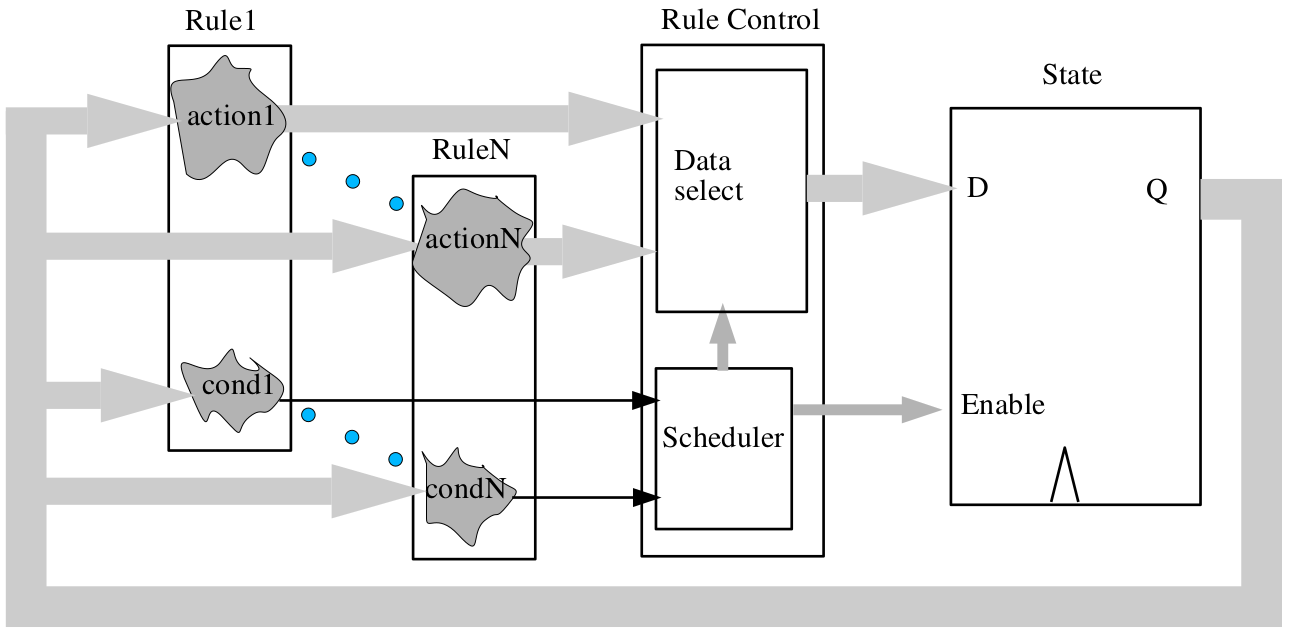
\includegraphics[width=\textwidth]{Figures/fig_MappingToHW.png}}
    \caption{%
        \label{fig_MappingToHW}
        A general scheme for mapping an N-rule system into clocked
        synchronous hardware.
    }
\end{figure}
Figure \ref{fig_MappingToHW} illustrates a general scheme to compose
rule components when mapping the design to clocked synchronous
hardware.  The State box lumps together all the state elements in the
{\BSV} design (as described earlier, state elements are explicitly
specified in {\BSV}).  The {\BSV} compiler produces a rule-control
circuit which conceptually takes all the enable (cond) signals and all
the data (action) outputs and controls which of the data outputs are
actually captured at the next clock in the state elements.  The enable
signals feed a \emph{scheduler} circuit that decides which of the
rules will actually fire.  The scheduler, in turn, controls data
multiplexers that select which data outputs reach the data inputs of
state elements, and controls which state elements are enabled to
capture the new data values.  Firing a rule simply means that the
scheduler selects its data output and clocks it into the next state.

At each clock, the scheduler selects a subset of rules to fire.  Not
all subsets are legal.  A subset is legal if and only if the rules in
the subset can be ordered with the following properties:
\begin{itemize}
\item
A hypothetical sequential execution of the ordered subset of rules is
legal at this point, according to the TRS semantics.  In particular,
the first rule in the ordered subset is currently enabled, and each
subsequent rule would indeed be enabled when execution reaches it in
the hypothetical sequence.

A special case is where all rules in the subset are already currently
enabled, and no rule would be disabled by execution of prior rules in
the order.

\item
The hardware execution produces the same net effect on the state as
the hypothetical sequential execution, even though the hardware
execution performs reads and writes in a different order from the
hypothetical sequential execution.

\end{itemize}
The {\BSV} compiler performs a very sophisticated analysis of the
rules in a design and synthesizes an efficient hardware scheduler that
controls execution in this manner.

Note that the scheme in Figure \ref{fig_MappingToHW} is for
illustrative purposes only.  First, it lumps together all the state,
shows a single rule-control box, etc., whereas in the real hardware
generated by the {\BSV} compiler these are distributed, localized and
modular.  Second, it is not the only way to map the design into
clocked synchronous hardware.  For example, any two enabled rules can
also be executed in a single clock by feeding the action outputs of
the first rule into the action inputs of the second rule, or by
synthesizing hardware for a composite circuit that computes the same
function as the composition of the two actions, and so on.  In
general, these alternative schemes may be more complex to analyze, or
may increase total propagation delay, but the compiler may use them in
special circumstances.

In summary, the {\BSV} compiler performs a detailed and sophisticated
analysis of rules and their interactions, and maps the design into
very efficient, highly parallel, clocked synchronous hardware
including a dynamic scheduler that allows many rules to fire in
parallel in each clock, but always in a manner that is consistent with
the reference TRS semantics.  The designer can use the simple
reference semantics to reason about correctness properties and be
confident that the synthesized parallel hardware will preserve those
properties. (See Section \ref{sec-rule-attributes} for the
``scheduling attributes'' mechanism using which the designer can guide
the compiler in implementing the mapping.)

When coding in other HDLs, the designer must maintain atomicity
manually.  He must recognize potential race conditions, and design the
appropriate data paths, control and synchronization to avoid them.
Reasoning about race conditions can cross module boundaries, and can
be introduced late in the design cycle as the problem specification
evolves.  The {\BSV} compiler automates all of this and, further, is
capable of producing RTL that is competitive with hand-coded RTL.

\subsubsection{How rules are chosen to fire}
\label{rule-choice}
The previous section described how an efficient circuit can be built
whose behavior will be consistent with sequential TRS semantics of {\BSV}.
However, as noted previously, the sequential reference semantics can be 
consistent with a range of different behaviors. There are two rule 
scheduling principles that guide the {\BSV} compiler in choosing 
which rules to schedule in a clock cycle (and help a designer build
circuits with predictable behavior). Except when overridden by an 
explicit user command or annotation, the {\BSV} compiler schedules 
rules according to the following two principles:

\begin{enumerate} 
\item Every rule enabled during a clock cycle will either be fired as part of
that clock cycle or a warning will be issued during compilation.
\item A rule will fire at most one time during a particular clock cycle.
\end{enumerate}

The first principle comes into play when two (or more) rules conflict - 
either because they are competing for a limited resource or because the result 
of their simultaneous execution is not consistent with any sequential rule 
execution. In the absence of a user annotation, the compiler will arbitrarily 
choose \footnote{The compiler's choice, while arbitrary, is deterministic. 
Given the same source and compiler version, the same schedule 
(and, hence, the same hardware) will be produced. However, because 
it is an arbitrary choice, it can be sensitive to otherwise irrelevant 
details of the program and is not guaranteed to remain the same if the 
source or compiler version changes.} 
which rule to prioritize, but \emph{must} also issue a warning. This guarantees 
the designer is aware of the ambiguity in the design and can correct it. It
might be corrected by changing the rules themselves (rearranging their predicates 
so they are never simultaneously applicable, for example) or by adding an urgency 
annotation which tells the compiler which rule to prefer (see section 
\ref{urgency-annotation}). When there are no scheduling warnings, it is 
guaranteed that the compiler is making no arbitrary choices about which rules to
execute.

The second principle ensures that continuously enabled rules (like a counter
increment rule) will not be executed an unpredictable number of times during
a clock cycle. According to the first rule scheduling principle, a rule that
is always enabled will be executed at least once during a clock cycle. However,
since the rule remains enabled it theoretically could execute multiple times 
in a clock cycle (since that behavior would be consistent with a sequential
semantics). Since rules (even simple things like a counter increment) consume
limited resources (like register write ports) it is pragmatically useful to 
restrict them to executing only once in a cycle (in the absence of specific
user instructions to the contrary). Executing a continuously enabled rule
only once in a cycle is also the more straightforward and intuitive behavior.

Together, these two principles allow a designer to completely determine the 
rules that will be chosen to fire by the schedule (and, hence, the behavior 
of the resulting circuit). 

\subsubsection{Mapping specific hardware models}

Annotations on the methods of a module
 are used by the BSV compiler to model the hardware behavior into TRS
 semantics. 
For example, all reads from a register must be scheduled before any
writes to the same register.  That is to say, any rule which reads
from a register must be scheduled \emph{earlier} than any other rule
which writes to it.  More generally, there exist scheduling
constraints for specific hardware modules which describe how methods
interact within the schedule.  The scheduling annotations
describe the constraints enforced by the BSV compiler.

\index{scheduling annotations}
\index{C@\te{C} (scheduling annotations)}
\index{CF@\te{CF} (scheduling annotations)}
\index{SB@\te{SB} (scheduling annotations)}
\index{SBR@\te{SBR} (scheduling annotations)}
\index{SA@\te{SA} (scheduling annotations)}
\index{SAR@\te{SAR} (scheduling annotations)}

\begin{tabbing}
The m\=eanings of \= the scheduling annotations are: \\
\\
\>\texttt{C} \> conflicts\\
\>\texttt{CF} \>      conflict-free \\
\>\texttt{SB} \>     sequence before \\
\>\texttt{SBR} \>     sequence before restricted (cannot be in the
same rule)\\
\>\texttt{SA} \>       sequence after\\
\>\texttt{SAR}\> sequence after restricted (cannot be in the same rule) 
\end{tabbing}

The annotations \te{SA} and \te{SAR} are provided for documentation
purposes only; they are not supported in the BSV language.

Below is an example of the scheduling annotations for a register:
\begin{center}
\begin{tabular}{|p{.75 in}|c|c|}
\hline
\multicolumn{3}{|c|}{Scheduling Annotations}\\
\multicolumn{3}{|c|}{Register }\\
\hline
&{read}&{write}\\
\hline
\hline
{read}&CF&SB\\
\hline
{write}&SA& SBR\\
\hline
\hline
\end{tabular}
\end{center}

The table  describes the following scheduling constraints:
\begin{itemize}
\item Two \te{read} methods would be
conflict-free (\te{CF}), that is, you could have multiple methods that
read from the same register in the same rule, sequenced in any order.
\item A \te{write} is sequenced  after (\te{SA}) a \te{read}.
\item A \te{read} is sequenced before (\te{SB}) a write. 
\item And
finally, if you have two \te{write} methods, one must be sequenced
before the other, and they cannot be in the same rule, as indicated by
the annotation \te{SBR}.  
\end{itemize}

The scheduling annotations are specific to the TRS model desired and a
single hardware component can have multiple TRS models.  For example,
a register may be implemented using a \te{mkReg} module or a
\te{mkConfigReg} module, which are identical except for their
scheduling annotations.  
% ================================================================

\section{User-defined types (type definitions)}

\label{sec-typedefs}
\index{typedef@\te{typedef} (keyword)}

User-defined types must be defined at the top level of  a package.

\gram{typeDef}{ \nterm{typedefSynonym} } \\
\gramalt      { \nterm{typedefEnum} }    \\
\gramalt      { \nterm{typedefStruct} }  \\
\gramalt      { \nterm{typedefTaggedUnion} }

As a matter of style, {\BSV} requires that all enumerations, structs
and unions be declared only via \texttt{typedef}, i.e., it is not possible
directly to declare a variable, formal parameter or formal argument as
an enum, struct or union without first giving that type a name using a
typedef.

Each typedef of an enum, struct or union introduces a new type that is
different from all other types.  For example, even if two typedefs
give names to struct types with exactly the same corresponding member
names and types, they define two distinct types.

Other typedefs, i.e., not involving an enum, struct or union, merely
introduce type synonyms for existing types.

% ----------------------------------------------------------------

\subsection{Type synonyms}
\label{sec-synonym}


Type synonyms are just for convenience and readability, allowing one
to define shorter or more meaningful names for existing types.  The
new type and the original type can be used interchangeably anywhere.

\gram{typedefSynonym}{ \term{typedef}  \nterm{type} \nterm{typeDefType} \term{;} }

\gram{typeDefType} {\nterm{typeIde} \opt{ \nterm{typeFormals}}

\gram{typeFormals}{\term{\#} \term{(} \nterm{typeFormal} \many{ \term{,} \nterm{typeFormal}}\term{)} }}

\gram{typeFormal}{\opt{\term{numeric} {\alt} \term{string}} \term{type} \nterm{typeIde}}


% \gram{typeDefType}{\nterm{typeIde} \opt{\term{\#} \term{(}
% \opt{\term{numeric}} \term{type} \nterm{typeIde} \many{ \term{,}
% \opt{\term{numeric}} \term{type} \nterm{typeIde}} \term{)}} }

Examples. Defining names for bit vectors of certain lengths:
\begin{verbatim}
 typedef bit [7:0]   Byte;
 typedef bit [31:0]  Word;
 typedef bit [63:0]  LongWord;
\end{verbatim}

Examples.  Defining names for polymorphic data types.
\begin{verbatim}
 typedef Tuple3#(a, a, a) Triple#(type a);

 typedef Int#(n) MyInt#(type n);
\end{verbatim}
The above example could also be written as:
\begin{verbatim}
 typedef Int#(n) MyInt#(numeric type n);
\end{verbatim}
The \te{numeric} is not required because the parameter to \te{Int} will always be numeric.
 \te{numeric} is only required when the compiler can't determine
 whether the parameter is a numeric or non-numeric type.  It will then
 default to assuming it is non-numeric.  The user can override this
 default by specifying \te{numeric} in the \te{typedef} statement.

A \te{typedef} statement can be used to define a synonym for an already
defined synonym.  Example:
\begin{verbatim}
 typedef Triple#(Longword) TLW;
\end{verbatim}

Since an Interface is a type, we can have nested types:
\begin{verbatim}
 typedef Reg#(Vector#(8, UInt#(8))) ListReg;
 typedef List#(List#(Bit#(4)))      ArrayOf4Bits;
\end{verbatim}

\index{Alias}
\index{NumAlias}

The \te{typedef} statement must always be at the top level of a
package, not within a module.  To introduce a local name within a
module, use \te{Alias} or \te{NumAlias} (see \LibRefGuide).  Since
these introduce new names which are type variables as opposed to
types, the new names must begin with lower case letters.
\te{NumAlias} is used to give new names to numeric types, while
\te{Alias} is used for types which can be the types of variables.
Example:

\begin{verbatim}
 module mkMod(Ifc)
   provisos (Alias#(Bit#(crc_size), crc));

 module mkRAM(RAMIfc)
   provisos (NumAlias#(addr_size, TLog#(buff_size)));
\end{verbatim}

% ----------------------------------------------------------------

\subsection{Enumerations}

\label{sec-enums}

\gram{typedefEnum}{ \term{typedef} \term{enum}
   \term{\{} \nterm{typedefEnumElements} \term{\}} \nterm{Identifier}
                    \opt{ \nterm{derives} }
                    \term{;} } \\
\gram{typedefEnumElements} { \nterm{typedefEnumElement} \many{ \term{,} \nterm{typedefEnumElement} }}\\
\gram{typedefEnumElement}{\nterm{Identifier} \opt{\term{=}
                    \nterm{intLiteral}}} \\
\gramalt{\nterm{Identifier}\term{[}\nterm{intLiteral}\term{]} \opt{\term{=}
\nterm{intLiteral}}} \\
\gramalt{\nterm{Identifier}\term{[}\nterm{intLiteral}\term{:}\nterm{intLiteral}\term{]} \opt{\term{=}
\nterm{intLiteral}}} \\


\index{enumerations}
\index{enum@\te{enum}}
Enumerations (enums) provide a way to define a set of unique symbolic
constants, also called \emph{labels} or \emph{member names}.  Each
enum definition creates a new type different from all other types.
% The newly defined labels must be unique (within a package), i.e., two
% different enums cannot use common labels.
Enum labels may be repeated in different enum definitions.
Enumeration labels must
begin with an uppercase letter.

The optional \nterm{derives} clause is discussed in more detail in
Sections \ref{sec-deriving-brief} and \ref{sec-overloading}. One
common form is \texttt{deriving (Bits)}, which tells the compiler to
generate a bit-representation for this enum.  Another common form of
the clause is \texttt{deriving (Eq)}, which tells the compiler to pick a
default equality operation for these labels, so they can also be
tested for equality and inequality.  A third common form is {\tt
deriving (Bounded)}, which tells the compiler to define constants {\tt
minBound} and \texttt{maxBound} for this type, equal in value to the
first and last labels in the enumeration.  Also defined in
\te{deriving (FShow)}, which defines a \te{Fmt} type for the labels
for use with \te{\$Display}  functions.  These specifications can be
combined, e.g., \texttt{deriving (Bits, Eq, Bounded, FShow)}.  All these default
choices for representation, equality and bounds can be overridden (see
Section {\ref{sec-overloading}}). 

The declaration may specify the encoding used by \texttt{deriving(Bits)}
by assigning numbers to tags.  When an assignment is omitted, the tag
receives an encoding of the previous tag incremented by one; when the
encoding for the initial tag is omitted, it defaults to zero.
Specifying the same encoding for more than one tag results in an
error.

Multiple tags may be declared by using the index
(\texttt{\emph{Tag}[\emph{ntags}]}) or range
(\texttt{\emph{Tag}[\emph{start}:\emph{end}]}) notation.  In the
former case, \emph{ntags} tags will be generated, from
\texttt{Tag0} to \texttt{Tag\emph{n-1}}; in the latter case,
$\left|\mathit{end}-\mathit{start}\right|+1$ tags, from
\texttt{Tag\emph{start}} to
\texttt{Tag\emph{end}}.

Example.  The boolean type can be defined in the language itself:
\begin{verbatim}
 typedef enum { False, True } Bool deriving (Bits, Eq);
\end{verbatim}
The compiler will pick a one-bit representation, with 1'b0 and 1'b1 as
the representations for \texttt{False} and \texttt{True}, respectively.  It
will define the \texttt{==} and \texttt{!=} operators to also work on {\tt
Bool} values.

Example. Excerpts from the specification of a processor:
\begin{verbatim}
 typedef enum { R0, R1, ..., R31 }  RegName deriving (Bits);
 typedef RegName  Rdest;
 typedef RegName  Rsrc;
\end{verbatim}
The first line defines an enum type with 32 register names.  The
second and third lines define type synonyms for \texttt{RegName} that may
be more informative in certain contexts (``destination'' and
``source'' registers).  Because of the \texttt{deriving} clause, the
compiler will pick a five-bit representation, with values 5'h00
through 5'h1F for \texttt{R0} through \texttt{R31}.

Example.  Tag encoding when \texttt{deriving(Bits)} can be specified manually:
\begin{verbatim}
 typedef enum {
   Add = 5,
   Sub = 0,
   Not,
   Xor = 3,
   ...
 } OpCode deriving (Bits);
\end{verbatim}
The \texttt{Add} tag will be encoded to five, \texttt{Sub} to zero, {\tt
Not} to one, and \texttt{Xor} to three.

Example.  A range of tags may be declared in a single clause:
\begin{verbatim}
 typedef enum {
   Foo[2],
   Bar[5:7],
   Quux[3:2]
 } Glurph;
\end{verbatim}
This is equivalent to the declaration
\begin{verbatim}
 typedef enum {
   Foo0,
   Foo1,
   Bar5,
   Bar6,
   Bar7,
   Quux3,
   Quux2
 } Glurph;
\end{verbatim}

% ----------------------------------------------------------------

\subsection{Structs and tagged unions}


\label{sec-struct-union-type}

A struct definition introduces a new record type.
\index{struct!type definition}
\index{union tagged!type definition}
\index{tagged union!type definition}
\index{struct@\verb'struct'}
\index{union@\verb'union'}
\index{tagged@\verb'tagged'|see{union}}
\index{records|see{struct}}

{\SV} has ordinary unions as well as tagged unions, but in {\BSV} we
only use tagged unions, for several reasons.  The principal benefit is
safety (verification).  Ordinary unions open a serious type-checking
loophole, whereas tagged unions are completely type-safe.  Other
reasons are that, in conjunction with pattern matching (Section
\ref{sec-patterns}), tagged unions yield much more succinct and
readable code, which also improves correctness.  In the text below, we
may simply say ``union'' for brevity, but it always means ``tagged
union.''

\gram{typedefStruct}{ \term{typedef} \term{struct}  \term{\{} } \\
\grammore           { \hmm \many{ \nterm{structMember} } } \\
\grammore           { \term{\}} \nterm{typeDefType} \opt{ \nterm{derives} } \term{;} }

\gram{typedefTaggedUnion}{ \term{typedef} \term{union} \term{tagged}  \term{\{} } \\
\grammore           { \hmm \many{ \nterm{unionMember} } } \\
\grammore           { \term{\}} \nterm{typeDefType} \opt{ \nterm{derives} } \term{;} }

\gram{structMember}{ \nterm{type} \nterm{identifier} \term{;} } \\
%\gramalt           { \nterm{subStruct} \nterm{identifier} \term{;} } \\
\gramalt           { \nterm{subUnion} \nterm{identifier} \term{;} }

\gram{unionMember}{ \nterm{type}      \nterm{Identifier} \term{;} } \\
\gramalt          { \nterm{subStruct} \nterm{Identifier} \term{;} } \\
\gramalt          { \nterm{subUnion} \nterm{Identifier} \term{;} } \\
\gramalt          { \term{void}       \nterm{Identifier} \term{;} }

\gram{subStruct}{ \term{struct} \term{\{} } \\
\grammore       { \hmm \many{ \nterm{structMember} } } \\
\grammore       { \term{\}} }

\gram{subUnion}{ \term{union} \term{tagged} \term{\{} } \\
\grammore       { \hmm \many{ \nterm{unionMember} } } \\
\grammore       { \term{\}} }

\gram{typeDefType} {\nterm{typeIde} \opt{ \nterm{typeFormals}}

\gram{typeFormals}{\term{\#} \term{(} \nterm{typeFormal} \many{ \term{,} \nterm{typeFormal}}\term{)} }}

\gram{typeFormal}{\opt{\term{numeric} {\alt} \term{string}} \term{type} \nterm{typeIde}}



All types can of course be mutually nested if mediated by typedefs,
but % structs and
unions can also be mutually nested directly, as
described in the syntax above.  Structs and unions contain
{\emph{members}}.  A union member (but not a struct member) can have
the special \texttt{void} type (see the types \texttt{MaybeInt} and {\tt
Maybe} in the examples below for uses of \texttt{void}).
\index{void@\texttt{void} (type, in tagged unions)}
All the member names in a particular struct or union must be unique,
but the same names can be used in other structs and members; the
compiler will try to disambiguate based on type.

A struct value contains the first member \emph{and} the second member
\emph{and} the third member, and so on.  A union value contains just
the first member \emph{or} just the second member \emph{or} just the
third member, and so on.  Struct member names must begin with a
lowercase letter, whereas union member names must begin with an
uppercase letter.

In a tagged union, the member names are also called \emph{tags}.  Tags
play a very important safety role.  Suppose we had the following:
\begin{verbatim}
 typedef union tagged { int Tagi; OneHot Tagoh; } U deriving (Bits);
 U  x;
\end{verbatim}
The variable \texttt{x} not only contains the bits corresponding to one
of its member types \texttt{int} or \texttt{OneHot}, but also some extra
bits (in this case just one bit) that remember the tag, 0 for {\tt
Tagi} and 1 for \texttt{Tagoh}.  When the tag is \texttt{Tagi}, it is
impossible to read it as a \texttt{OneHot} member, and when the tag is
\texttt{Tagoh} it is impossible to read it as an \texttt{int} member, i.e.,
the syntax and type checking ensure this.  Thus, it is impossible
accidentally to misread what is in a union value.

The optional \nterm{derives} clause is discussed in more detail in
Section \ref{sec-overloading}.  One common form is \texttt{deriving
(Bits)}, which tells the compiler to pick a default bit-representation
for the struct or union.  For structs it is simply a concatenation of
the representations of the members.  For unions, the representation
consists of $t+m$ bits, where $t$ is the minimum number of bits to
code for the tags in this union and $m$ is the number of bits for the
largest member.  Every union value has a code in the $t$-bit field
that identifies the tag, concatenated with the bits of the
corresponding member, right-justified in the $m$-bit field.  If the
member needs fewer than $m$ bits, the remaining bits (between the tag
and the member bits) are undefined.

Struct and union typedefs can define new, polymorphic types, signalled
by the presence of type parameters in \texttt{\#(...)}. Polymorphic
types are discussed in section \ref{sec-polymorphism-brief}.

Section \ref{sec-struct-union-exprs} on struct and union expressions
describes how to construct struct and union values and to access and
update members.  Section \ref{sec-patterns} on pattern-matching
describes a more high-level way to access members from structs and
unions and to test union tags.

Example. Ordinary, traditional record structures:
\begin{verbatim}
 typedef struct { int x; int y; } Coord;
 typedef struct { Addr pc; RegFile rf; Memory mem; }  Proc;
\end{verbatim}

Example. Encoding instruction operands in a processor:
\begin{verbatim}
 typedef union tagged {
     bit  [4:0] Register;
     bit [21:0] Literal;
     struct {
         bit  [4:0] regAddr;
         bit  [4:0] regIndex;
     } Indexed;
 } InstrOperand;
\end{verbatim}
An instruction operand is either a 5-bit register specifier, a 22-bit
literal value, or an indexed memory specifier, consisting of two 5-bit
register specifiers.

Example.  Encoding instructions in a processor:
\begin{verbatim}
 typedef union tagged {
    struct {
        Op op; Reg rs; CPUReg rt; UInt16 imm;
    } Immediate;

    struct {
        Op op; UInt26 target;
    } Jump;
 } Instruction
   deriving (Bits);
\end{verbatim}
An \texttt{Instruction} is either an \texttt{Immediate} or a \texttt{Jump}.
In the former case, it contains
a field, \texttt{op}, containing a value of type \texttt{Op};
a field, \texttt{rs}, containing a value of type \texttt{Reg};
a field, \texttt{rt}, containing a value of type \texttt{CPUReg}; and
a field, \texttt{imm}, containing a value of type \texttt{UInt16}.
In the latter case, it contains
a field, \texttt{op}, containing a value of type \texttt{Op}, and
a field, \texttt{target}, containing a value of type \texttt{UInt26}.

Example. Optional integers (an integer together with a valid bit):
\begin{verbatim}
 typedef union tagged {
     void    Invalid;
     int     Valid;
 } MaybeInt
   deriving (Bits);
\end{verbatim}
A \texttt{MaybeInt} is either invalid, or it contains an
integer (Valid tag).  The representation of this type will be 33 bits---
one bit to represent \texttt{Invalid} or \texttt{Valid} tag, plus 32 bits for an
\texttt{int}.  When it carries an invalid value, the remaining 32 bits
are undefined.  It will be impossible to read/interpret those 32 bits
when the tag bit says it is \texttt{Invalid}.

This \texttt{MaybeInt} type is very useful, and not just for integers.
We generalize it to a polymorphic type:
\begin{verbatim}
 typedef union tagged {
     void  Invalid;
     a     Valid;
 } Maybe#(type a)
   deriving (Bits);
\end{verbatim}
This \texttt{Maybe} type can be used with any type \texttt{a}.
\index{Maybe@\te{Maybe} (type)}
\index{Invalid@\te{Invalid}!tagged union member of\texttt{Maybe} type}
\index{Valid@\te{Valid}!tagged union member of\texttt{Maybe} type}
Consider a function that, given a key, looks up a table and returns
some value associated with that key.  Such a function can return
either an invalid result (\texttt{Invalid}), if the table does not
contain an entry for the given key, or a valid result \texttt{Valid~$v$}
if $v$ is associated with the key in the table.  The type is
polymorphic (type parameter \texttt{a}) because it may be used with
lookup functions for integer tables, string tables, IP address tables,
etc.  In other words, we do not over-specify the type of the value $v$
at which it may be used.

See Section \ref{sec-tuple-type} for an important, predefined set of
struct types called \emph{Tuples} for adhoc structs of between two and
eight members.

% ================================================================

\section{Type classes (overloading groups) and provisos}

\label{sec-overloading}

\index{overloading, of types}
\index{type classes}
\index{overloading groups|see {type classes}}

\emph{Note: This is an advanced topic that may be skipped on first reading.}

For most {\BSV} programming, one just needs to know about a few
predefined type classes such as \texttt{Bits} and \texttt{Eq}, about
provisos, and about the automatic mechanism for defining the
overloaded functions in those type classes using a \texttt{deriving}
clause.  The brief introduction in Sections \ref{sec-provisos-brief}
and \ref{sec-deriving-brief} should suffice.

This section is intended for the advanced programmer who may wish to
define new type classes (using a \texttt{typeclass} declaration), or
explicitly to define overloaded functions using an \texttt{instance}
declaration.

In programming languages, the term \emph{overloading} refers to the
use of a common function name or operator symbol to represent some
number (usually finite) of functions with distinct types.  For
example, it is common to overload the operator symbol \texttt{+} to
represent integer addition, floating point addition, complex number
addition, matrix addition, and so on.

Note that overloading is distinct from \emph{polymorphism}, which is
used to describe a single function or operator that can operate at an
infinity of types.  For example, in many languages, a single
polymorphic function \texttt{arraySize()} may be used to determine the
number of elements in any array, no matter what the type of the
contents of the array.

A \emph{type class} (or \emph{overloading group}) further recognizes
that overloading is often performed with related groups of function
names or operators, giving the group of related functions and
operators a name.  For example, the type class \texttt{Ord} contains the
overloaded operators for order-comparison: \texttt{<}, \texttt{<=}, \texttt{>}
and \texttt{>=}.
\index{Ord@\te{Ord} (type class)}
\index{type classes!\te{Ord}}

If we specify the functions represented by these operator symbols for
the types \texttt{int}, \texttt{Bool}, \texttt{bit[$m$:0]} and so on, we say
that those types are \emph{instances} of the \texttt{Ord} type class.
\index{instance of type class (overloading group)}

A \emph{proviso} is a (static) condition attached to some constructs.
A proviso requires that certain types involved in the construct must
be instances of certain type classes.  For example, a generic {\tt
sort} function for sorting lists of type \texttt{List\#($t$)} will have a
proviso (condition) that $t$ must be an instance of the \texttt{Ord} type
class, because the generic function uses an overloaded comparison
operator from that type class, such as the operator \texttt{<} or \texttt{>}.
\index{Ord@\te{Ord} (type class)}

Type classes are created explicitly using a \texttt{typeclass}
declaration (Section \ref{sec-typeclass-def}).  Further, a type class
is explicitly populated with a new instance type $t$, using an {\tt
instance} declaration (Section {\ref{sec-instance-def}}), in which the
programmer provides the specifications for the overloaded functions
for the type $t$.

% ----------------------------------------------------------------

\subsection{Provisos}

\label{sec-provisos}

\index{provisos}
Consider the following function prototype:
\begin{verbatim}
 function List#(t) sort (List#(t) xs)
     provisos (Ord#(t));
\end{verbatim}
\index{Ord@\te{Ord} (type class)}
This prototype expresses the idea that the sorting function takes an
input list \texttt{xs} of items of type \texttt{t} (presumably unsorted),
and produces an output list of type \texttt{t} (presumably sorted).  In
order to perform its function it needs to compare elements of the list
against each other using an overloaded comparison operator such as
\texttt{<}.  This, in turn, requires that the overloaded operator be
defined on objects of type \texttt{t}. This is exactly what is expressed
in the proviso, i.e., that \texttt{t} must be an instance of the type
class (overloading group) \texttt{Ord}, which contains the overloaded
operator \texttt{<}.
\index{Ord@\te{Ord} (type class)}

Thus, it is permissible to apply \texttt{sort} to lists of \texttt{Integer}s
or lists of \texttt{Bool}s, because those types are instances of {\tt
Ord},
\index{Ord@\te{Ord} (type class)}
but it is not permissible to apply \texttt{sort} to a list of, say,
some interface type \texttt{Ifc} (assuming \texttt{Ifc} is not an instance
of the \texttt{Ord} type class).

The syntax of provisos is the following:

\gram{provisos}{ \term{provisos}
                     \term{(}
                     \nterm{proviso}  \many{ \term{,} \nterm{proviso} }
                     \term{)} }

\gram{proviso}{ \nterm{Identifier} \term{\#}\term{(}\nterm{type} \many{
                     \term{,} \nterm{type} } \term{)} }

In each \nterm{proviso}, the \nterm{Identifier} is the name of type
class (overloading group).  In most provisos, the type class name $T$
is followed by a single type $t$, and can be read as a simple
assertion that $t$ is an instance of $T$, i.e., that the overloaded
functions of type class $T$ are defined for the type $t$.  In some
provisos the type class name $T$ may be followed by more than one type
$t_1$, ..., $t_n$ and these express more general relationships.  For
example, a proviso like this:
\begin{verbatim}
     provisos (Bits#(macAddress, 48))
\end{verbatim}
can be read literally as saying that the types \texttt{macAddress} and
\texttt{48} are in the \texttt{Bits} type class, or can be read more
generally as saying that values of type \texttt{macAddress} can be
converted to and from values of the type \texttt{bit[47:0]} using the
\texttt{pack} and \texttt{unpack} overloaded functions of type class {\tt
Bits}.

\index{context|see {provisos}}
We sometimes also refer to provisos as \emph{contexts}, meaning that
they constrain the types that may be used within the construct to
which the provisos are attached.

Occasionally, if the context is too weak, the compiler may be unable
to figure out how to resolve an overloading.
\index{context too weak (overloading resolution)}
Usually the compiler's error message will be a strong hint about what
information is missing.  In these situations it may be necessary for
the programmer to guide the compiler by adding more type information
to the program, in either or both of the following ways:
\begin{itemize}

\item
Add a static type assertion (Section \ref{sec-static-type-assertions})
to some expression that narrows down its type.

\item
Add a proviso to the surrounding construct.

\end{itemize}

% ----------------------------------------------------------------

\subsection{Type class declarations}

\label{sec-typeclass-def}
\index{type classes!\te{typeclass} (declaring new)}

A new class is declared using the following syntax:

\gram{typeclassDef}{ \term{typeclass} \nterm{typeclassIde}
                                      \nterm{typeFormals}
                                      \opt{ \nterm{provisos}}} \\
\grammore                  { \opt {\nterm{typedepends}} \term{;} } \\
%                                      \term{;} } \\
\grammore          { \hmm \many{ \nterm{overloadedDef} } } \\
\grammore          { \term{endtypeclass} \opt{: \nterm{typeclassIde} } }

\gram{typeclassIde}{ \nterm{Identifier} }

\gram{typeFormals}{\term{\#} \term{(} \nterm{typeFormal} \many{ \term{,} \nterm{typeFormal}}\term{)} }

\gram{typeFormal}{\opt{\term{numeric} {\alt} \term{string}} \term{type} \nterm{typeIde}}

\gram{typedepends}          {\term{dependencies} \term{(}
                                             \nterm{typedepend} \many
                                             {\term{,}
                                             \nterm{typedepend}}
                                             \term{)}}

\gram{typedepend}           {\nterm{typelist} \term{determines} \nterm{typelist}}


\gram{typelist}             {\nterm{typeIde}} \\
\gramalt                    {\term{(} \nterm{typeIde} \many {\term{,}
                                             \nterm{typeIde}} \term{)} }

\gram{overloadedDef}{ \nterm{functionProto} } \\
\gramalt            { \nterm{varDecl} }

The {\nterm{typeclassIde}} is the newly declared class name.  The
{\nterm{typeFormals}} represent the types that will be instances of
this class.  These {\nterm{typeFormals}} may themselves be constrained
by {\nterm{provisos}}, in which case the classes named in
{\nterm{provisos}} are called the ``super type classes'' of this type
class.  Type dependencies (\nterm{typedepends}) are relevant only if there are
two or more \nterm{type} parameters; the \nterm{typedepends} comes after the
typeclass's provisos (if any) and before the semicolon. The
{\nterm{overloadedDef}s} declare the overloaded variables or function
names,  and their types.

Example (from the Standard Prelude package):
\index{Standard Prelude}
\begin{verbatim}
 typeclass Literal#(type a);
     function a    fromInteger (Integer x);
     function Bool inLiteralRange(a target, Integer i);
 endtypeclass: Literal
\end{verbatim}
This defines the type class \texttt{Literal}.  Any type \texttt{a} that is
an instance of \texttt{Literal} must have an overloaded function called
\texttt{fromInteger} that converts an \texttt{Integer} value into the type
\texttt{a}.  In fact, this is the mechanism that {\BSV} uses to interpret
integer literal constants, e.g., to resolve whether a literal like
\texttt{6847} is to be interpreted as a signed integer, an unsigned
integer, a floating point number, a bit value of 10 bits, a bit value
of 8 bits, etc.  (See Section \ref{sec-typeconv-integer-literals} for
a more detailed description.). 

The typeclass also provides a function \texttt{inLiteralRange} that takes
an argument of type \texttt{a} and an \texttt{Integer} and returns a 
\texttt{Bool}. In the standard \texttt{Literal} typeclass this boolean
indicates whether or not the supplied \texttt{Integer} is in the range
of legal values for the type \texttt{a}.
 
Example (from a predefined type class in {\BSV}):
\begin{verbatim}
 typeclass Bounded#(type a);
     a minBound;
     a maxBound;
 endtypeclass
\end{verbatim}
This defines the type class \texttt{Bounded}.  Any type \texttt{a} that is
an instance of \texttt{Bounded} will have two values called {\tt
minBound} and \texttt{maxBound} that, respectively, represent the minimum
and maximum of all values of this type.

Example (from a predefined type class in {\BSV}):\footnote{ We are
using {\V}'s notation for \emph{escaped identifiers} to treat operator
symbols as ordinary identifiers.  The notation allows an identifier to
be constructed from arbitrary characters beginning with a backslash
and ending with a whitespace (the backslash and whitespace are not
part of the identifier.)}
\begin{verbatim}
   typeclass Arith #(type data_t)
     provisos (Literal#(data_t));
       function data_t \+ (data_t x, data_t y);
       function data_t \- (data_t x, data_t y);
       function data_t negate (data_t x);
       function data_t \* (data_t x, data_t y);
       function data_t \/ (data_t x, data_t y);
       function data_t \% (data_t x, data_t y);
   endtypeclass
\end{verbatim}
This defines the type class \texttt{Arith} with super type class {\tt
Literal}, i.e., the proviso states that in order for a type \texttt{data\_t} to
be an instance of \texttt{Arith} it must also be an instance of the type
class \texttt{Literal}.  Further, it has six overloaded functions with
the given names and types.  Said another way, a type that is an
instance of the \texttt{Arith} type class must have a way to convert
integer literals into that type, and it must have addition,
subtraction, negation, multiplication, and division defined on it.

The
semantics of a dependency say that once the types on the left of the
\te{determines} keyword are fixed, the types on the right are 
uniquely  determined.  The types on either side of the list can be a
single type or a list of types, in which case they are enclosed in
parentheses.

Example of a typeclass definition specifying type dependencies:
\begin{verbatim}
typeclass Connectable #(type a, type b)
    dependencies (a determines b, b determines a);
       module mkConnection#(a x1, b x2) (Empty);
endtypeclass
\end{verbatim}

For any type \texttt{t} we know that \texttt{Get\#(t)}
and \texttt{Put\#(t)} are connectable because of the following
declaration in the \te{GetPut} package: 
\begin{verbatim}
instance Connectable#(Get#(element_type), Put#(element_type));
\end{verbatim}

In the \te{Connectable} dependency above, it states that \te{a}
determines \te{b}.  Therefore, you know
that if \te{a} is \te{Get\#(t)}, the \emph{only} possibility for \te{b} is
 \te{Put\#(t)}.

% (because there's an instance
% declaration in the \te{GetPut} package that says so); then the
% dependency specification above says that if you know that \te{a} is
% \te{Get\#(t)}, the \emph{only} possibility for \te{b} is
% \te{Put\#(t)


Example of a typeclass definition with lists of types in the dependencies:
\begin{verbatim}
typeclass Extend #(type a, type b, type c)
    dependencies ((a,c) determines b, (b,c) determines a); 
endtypeclass
\end{verbatim}


An example of a case where the dependencies are not commutative:
\begin{verbatim}
typeclass Bits#(type a, type sa)
   dependencies (a determines sa);
      function Bit#(sa) pack(a x);
      function a unpack (Bit#(sa) x);
endtypeclass
\end{verbatim}
In the above example, if \te{a} were \te{UInt\#(16)} the dependency
would require that \te{b} had to be 16; but the fact that something
occupies 16 bits by no means implies that it has to be a \te{UInt}.


% ----------------------------------------------------------------

\subsection{Instance declarations}

\label{sec-instance-def}

\index{type classes!instance declaration}
\index{type classes!\te{instance}}

\index{instance@\te{instance}}
\index{instance of type class (overloading group)}

A type can be declared to be an instance of a class in two ways, with
a general mechanism or with a convenient shorthand.  The general
mechanism of \texttt{instance} declarations is the following:

\gram{typeclassInstanceDef}{ \term{instance} \nterm{typeclassIde}
                                 \term{\#} \term{(}
                                             \nterm{type} \many{ \term{,} \nterm{type} }
                                           \term{)}
                                             \opt{\nterm{provisos}} \term{;}} \\
%\grammore                  { \opt {\nterm{typedepends}} \term{;} } \\
\grammore                  { \hmm \many{ \nterm{varAssign} \term{;}
                                             {\alt}
                                             \nterm{functionDef} 
                                             {\alt}
                                             \nterm{moduleDef} }}
                                             \\
\grammore                  { \term{endinstance} \opt{ \term{:}  \nterm{typeclassIde} } }

% \gram{typedepends}          {\term{dependencies} \term{(}
%                                              \nterm{typedepend} \many
%                                              {\term{,}
%                                              \nterm{typedepend}}
%                                              \term{)}}

% \gram{typedepend}           {\nterm{type} \term{determines} \nterm {type}} 

This says that the {\nterm{type}}s are an instance of type class
{\nterm{typeclassIde}} with the given provisos.  The
{\nterm{varAssign}}s, {\nterm{functionDef}}s and {\nterm{moduleDef}}s specify the
implementation of the overloaded identifiers of the type class. 


Example, declaring a type as an instance of the \texttt{Eq} typeclass:
\begin{verbatim}
typedef enum { Red, Blue, Green } Color;

instance Eq#(Color);
  function Bool \== (Color x, Color y); //must use \== with a trailing 
    return True;                        //space to define custom instances    
  endfunction                           //of the Eq typeclass
endinstance
\end{verbatim}

The shorthand mechanism is to attach a \texttt{deriving} clause to a
typedef of an enum, struct or tagged union and let the compiler do the
work.  In this case the compiler chooses the ``obvious''
implementation of the overloaded functions (details in the following
sections).  The only type classes for which \texttt{deriving} can be used
for general types are \texttt{Bits}, \texttt{Eq}, \texttt{Bounded},
and \texttt{FShow}.
Furthermore, \texttt{deriving} can be used for any class if the type is a
data type that is isomorphic to a type that has an instance for the
derived class.

\gram{derives}{ \term{deriving} \term{(} \nterm{typeclassIde}
                                         \many{ \term{,} \nterm{typeclassIde} }
                                \term{)} }

Example:
\begin{verbatim}
typedef enum { Red, Blue, Green } Color deriving (Eq);
\end{verbatim}


% ----------------------------------------------------------------

\subsection{The \texttt{Bits} type class (overloading group)}

\label{sec-Bits-typeclass}

\index{Bits@\te{Bits} (type class)}
\index{type classes!\te{Bits}}

The type class \texttt{Bits} contains the types that are convertible to
bit strings of a certain size.  Many constructs have membership in the
\texttt{Bits} class as a proviso, such as putting a value into a
register, array, or FIFO.

Example: The \texttt{Bits} type class definition (which is actually
predefined in {\BSV}) looks something like this:
\begin{verbatim}
 typeclass Bits#(type a, type n);
     function  Bit#(n)  pack   (a x);
     function  a        unpack (Bit#(n) y);
 endtypeclass
\end{verbatim}
\index{pack@\texttt{pack} (\texttt{Bits} type class overloaded function)}
\index{unpack@\texttt{unpack} (\texttt{Bits} type class overloaded function)}
Here, \texttt{a} represents the type that can be converted to/from bits,
and \texttt{n} is always instantiated by a size type (Section
{\ref{sec-type}}) representing the number of bits
needed to represent it.  Implementations of modules such as registers
and FIFOs use these functions to convert between values of other types
and the bit representations that are really stored in those elements.

Example:  The most trivial instance declaration states that a
bit-vector can be converted to a bit vector, by defining both the \texttt{
pack} and \texttt{unpack} functions to be identity functions:
\begin{verbatim}
 instance Bits#(Bit#(k), k);
     function Bit#(k) pack (Bit#(k) x);
         return x;
     endfunction: pack

     function Bit#(k) unpack (Bit#(k) x);
         return x;
     endfunction: unpack
 endinstance
\end{verbatim}
Example:
\begin{verbatim}
 typedef enum { Red, Green, Blue } Color deriving (Eq);

 instance Bits#(Color, 2);
     function Bit#(2) pack (Color c);
         if      (c == Red)   return 3;
         else if (c == Green) return 2;
         else                 return 1;   // (c == Blue)
     endfunction: pack

     function Color unpack (Bit#(2) x);
         if      (x == 3) return Red;
         else if (x == 2) return Green;
         else if (x == 1) return Blue;
         else ? //Illegal opcode; return unspecified value
     endfunction: unpack
 endinstance
\end{verbatim}
% Bogus $ sign in this comment to match the one in the error stmt above
% to unconfuse LaTeX-mode in Emacs
Note that the \texttt{deriving (Eq)} phrase permits us to use the
equality operator \texttt{==} on \texttt{Color} types in the \texttt{pack}
function.  \texttt{Red}, \texttt{Green} and \texttt{Blue} are coded as 3, 2 and
1, respectively.  If we had used the \texttt{deriving(Bits)} shorthand in
the \texttt{Color} typedef, they would have been coded as 0, 1 and 2,
respectively (Section \ref{sec-deriving-Bits}).

% ----------------------------------------------------------------

\subsection{The \texttt{SizeOf} pseudo-function}

\label{sec-sizeof}

\index{SizeOf@\texttt{SizeOf} (pseudo-function on types)}
The pseudo-function \texttt{SizeOf\#($t$)} can be applied to a type $t$ to
get the numeric type representing its bit size.  The type $t$ must be
in the \texttt{Bits} class, i.e., it must already be an instance of {\tt
Bits\#($t$,$n$)}, either through a \texttt{deriving} clause or through an
explicit instance declaration.  The \texttt{SizeOf} function then returns
the corresponding bit size $n$.  Note that \texttt{SizeOf} returns a
numeric type, not a numeric value, i.e., the output of \texttt{SizeOf}
can be used in a type expression, and not in a value expression.

\texttt{SizeOf}, which converts a type to a (numeric) type, should not be
confused with the pseudo-function \texttt{valueof}, described in Section
{\ref{sec-valueof}}, which converts a numeric type to a numeric value.

Example:
\begin{verbatim}
 typedef Bit#(8) MyType;
 // MyType is an alias of Bit#(8)

 typedef SizeOf#(MyType) NumberOfBits;
 // NumberOfBits is a numeric type, its value is 8

 Integer ordinaryNumber = valueOf(NumberOfBits);
 // valueOf converts a numeric type into Integer 
\end{verbatim}

% ----------------------------------------------------------------

\subsection{Deriving \texttt{Bits}}

\label{sec-deriving-Bits}

\index{deriving@\texttt{deriving}!\texttt{Bits}}
\index{Bits@\te{Bits} (type class)!\texttt{deriving}}
\index{Bits@\te{Bits} (type class)!representation of data types}
\index{type classes!\te{Bits}}
When attaching a \texttt{deriving(Bits)} clause to a user-defined type,
the instance derived for the \texttt{Bits} type class can be described as
follows:
\begin{itemize}

\item
For an enum type it is simply an integer code, starting with zero for
the first enum constant and incrementing by one for each subsequent
enum constant.  The number of bits used is the minimum number of bits
needed to represent distinct codes for all the enum constants.

\item
For a struct type it is simply the concatenation of the bits for all
the members.  The first member is in the leftmost bits (most
significant) and the last member is in the rightmost bits (least
significant).

\item
For a tagged union type, all values of the type occupy the same number
of bits, regardless of which member it belongs to.  The bit
representation consists of two parts---a tag on the left (most
significant) and a member value on the right (least significant).

The tag part uses the minimum number of bits needed to code for all
the member names.  The first member name is given code zero, the next
member name is given code one, and so on.

The size of the member value part is always the size of the largest
member.  The member value is stored in this field, right-justified
(i.e., flush with the least-significant end). If the member value
requires fewer bits than the size of the field, the intermediate bits
are don't-care bits.

\end{itemize}

Example. Symbolic names for colors:
\begin{verbatim}
 typedef enum { Red, Green, Blue } Color deriving (Eq, Bits);
\end{verbatim}
This is the same type as in Section {\ref{sec-Bits-typeclass}} except
that \texttt{Red}, \texttt{Green} and \texttt{Blue} are now coded as 0, 1 and
2, instead of 3, 2, and 1, respectively, because the canonical choice
made by the compiler is to code consecutive labels incrementing from
0.

Example.  The boolean type can be defined in the language itself:
\begin{verbatim}
 typedef enum { False, True} Bool deriving (Bits);
\end{verbatim}
The type \texttt{Bool} is represented with one bit.  \texttt{False} is
represented by 0 and \texttt{True} by 1.

Example.  A struct type:
\begin{verbatim}
 typedef struct { Bit#(8) foo; Bit#(16) bar } Glurph deriving (Bits);
\end{verbatim}
The type \texttt{Glurph} is represented in 24 bits, with \texttt{foo} in the
upper 8 bits and \texttt{bar} in the lower 16 bits.

Example.  Another struct type:
\begin{verbatim}
 typedef struct{ int x; int y } Coord deriving (Bits);
\end{verbatim}
The type \texttt{Coord} is represented in 64 bits, with \texttt{x} in the
upper 32 bits and \texttt{y} in the lower 32 bits.

Example.  The \texttt{Maybe} type from Section \ref{sec-struct-union-type}:
\begin{verbatim}
 typedef union tagged {
     void  Invalid;
     a     Valid;
 } Maybe#(type a)
   deriving (Bits);
\end{verbatim}
is represented in $1+n$ bits, where $n$ bits are needed to represent
values of type \texttt{a}.  If the leftmost bit is 0 (for \texttt{Invalid})
the remaining $n$ bits are unspecified (don't-care).  If the leftmost
bit is 1 (for \texttt{Valid}) then the remaining $n$ bits will contain a
value of type \texttt{a}.

% ----------------------------------------------------------------

\subsection{Deriving \texttt{Eq}}

\label{sec-deriving-Eq}

\index{deriving@\texttt{deriving}!\texttt{Eq}}
\index{Eq@\te{Eq} (type class)!\texttt{deriving}}
\index{type classes!\te{Eq}}

The \texttt{Eq} type class contains the overloaded operators \texttt{==}
(logical equality) and \texttt{!=} (logical inequality):
\begin{verbatim}
 typeclass Eq#(type a);
     function Bool \== (a x1, a x2);
     function Bool \/= (a x1, a x2);
 endtypeclass: Eq
\end{verbatim}

When \texttt{deriving(Eq)} is present on a a user-defined type definition
$t$, the compiler defines these equality/inequality operators for
values of type $t$.  It is the natural recursive definition of these
operators, i.e.,
\begin{itemize}

\item
If $t$ is an enum type, two values of type $t$ are equal if they
represent the same enum constant.

\item
If $t$ is a struct type, two values of type $t$ are equal if the
corresponding members are pairwise equal.

\item
If $t$ is a tagged union type, two values of type $t$ are equal if
they have the same tag (member name) and the two corresponding member
values are equal.

\end{itemize}

% ----------------------------------------------------------------

\subsection{Deriving \texttt{Bounded}}

\label{sec-deriving-Bounded}

\index{deriving@\texttt{deriving}!\texttt{Bounded}}
\index{Bounded@\te{Bounded} (type class)!\texttt{deriving}}
\index{type classes!\te{Bounded}}

The predefined type class \texttt{Bounded} contains two overloaded
identifiers \texttt{minBound} and \texttt{maxBound} representing the minimum
and maximum values of a type \texttt{a}:
\begin{verbatim}
 typeclass Bounded#(type a);
     a minBound;
     a maxBound;
 endtypeclass
\end{verbatim}

The clause \texttt{deriving(Bounded)} can be attached to any user-defined
enum definition $t$, and the compiler will define the values {\tt
minBound} and \texttt{maxBound} for values of type $t$ as the first and
last enum constants, respectively.

The clause \texttt{deriving(Bounded)} can be attached to any user-defined
struct definition $t$ with the proviso that the type of each member is
also an instance of \texttt{Bounded}.  The compiler-defined {\tt
minBound} (or \texttt{maxBound}) will be the struct with each member
having its respective \texttt{minBound} (respectively, \texttt{maxBound}).

% ----------------------------------------------------------------

\subsection{Deriving \texttt{FShow}}

\label{sec-deriving-FShow}
\index{deriving@\texttt{deriving}!\texttt{FShow}}
\index{FShow@\te{FShow} (type class)!\texttt{deriving}}
\index{type classes!\te{FShow}}

The  intent of the \te{FShow} type class is to format values for
use with  the \te{\$display} family of functions.

When attaching a \te{deriving(FShow)} clause to a user-defined type,
the instance derived for the \te{FShow} type class can be described as
follows:

\begin{itemize}

\item For an enum type, the output contains the enumerated value.

Example:
\begin{verbatim}
typedef enum { Red, Blue, Green } Colors deriving (FShow);
...
      $display("Basic enum");
      Colors be0 = Red;
      Colors be1 = Blue;
      Colors be2 = Green;
      $display(fshow(be0));
      $display(fshow(be1));
      $display(fshow(be2));
\end{verbatim}

Displays:
\begin{verbatim}
Basic enum
Red
Blue
Green
\end{verbatim}

\item For a struct type, the output contains the struct name, with
each value prepended with the name of the field.  The values are
formatted with \te{FShow} according to the data type.
\begin{verbatim}
   Struct_name {field1_name: value1, field2_name: value2....}
\end{verbatim}

Example:

\begin{verbatim}
typedef struct {
   Bool      val_bool;
   Bit#(8)   val_bit;
   UInt#(16) val_uint;
   Int#(32)  val_int;
} BasicS deriving (FShow);
...
      $display("Basic struct");
      BasicS bs1 =
          BasicS { val_bool: True, val_bit: 22,
                   val_uint: 'hABCD, val_int: -'hABCD };
      $display(fshow(bs1));
\end{verbatim}

Displays:
\begin{verbatim}
Basic struct
BasicS { val_bool: True, val_bit: 'h16, val_uint: 43981, val_int:      -43981 }
\end{verbatim}

\item For a tagged union type, the output contains the name of the tag
followed by the value.  The values are
formatted with \te{FShow} according to the data type.

\begin{verbatim}
   tagged Tag1 value1
   tagged Tag2 value2
\end{verbatim}

Example:
\begin{verbatim}
typedef union tagged {
   Bool      Val_bool;
   Bit#(8)   Val_bit;
   UInt#(16) Val_uint;
   Int#(32)  Val_int;
} BasicU deriving (FShow);
...
      $display("Basic tagged union");
      BasicU bu0 = tagged Val_bool True;
      BasicU bu1 = tagged Val_bit 22;
      BasicU bu2 = tagged Val_uint 'hABCD;
      BasicU bu3 = tagged Val_int -'hABCD;
      $display(fshow(bu0));
      $display(fshow(bu1));
      $display(fshow(bu2));
      $display(fshow(bu3));
\end{verbatim}

Displays:

\begin{verbatim}
Basic tagged union
tagged Val_bool True
tagged Val_bit  'h16
tagged Val_uint 43981
tagged Val_int      -43981
\end{verbatim}

\end{itemize}

% ----------------------------------------------------------------

\subsection{Deriving type class instances for isomorphic types}

\index{deriving@\texttt{deriving}!for isomorphic types}
Generally speaking, the \texttt{deriving(...)} clause can only be used
for the predefined type classes \texttt{Bits}, \texttt{Eq}, {\tt
Bounded}, and {\tt FShow}.  However there is a special case where it can be used for
any type class.  When a user-defined type $t$ is \emph{isomorphic} to
an existing type $t'$, then all the functions on $t'$ automatically
work on $t$, and so the compiler can trivially derive a function for
$t$ by just using the corresponding function for $t'$.

There are two situations where a newly defined type is isomorphic to
an old type: a struct or tagged union with precisely one member. For
example:

\begin{tabbing}
\hm \texttt{typedef struct \{} $t'$ \texttt{x; \}} $t$ \texttt{deriving (}\emph{anyClass}\texttt{);} \\
\hm \texttt{typedef union tagged \{} $t'$ \texttt{X; \}} $t$ \texttt{deriving (}\emph{anyClass}\texttt{);} \\
\end{tabbing}

One sometimes defines such a type precisely for type-safety reasons
because the new type is distinct from the old type although isomorphic
to it, so that it is impossible to accidentally use a $t$ value in a
$t'$ context and vice versa.  Example:
\begin{verbatim}
 typedef struct { UInt#(32) x; } Apples deriving (Literal, Arith);
 ...
 Apples five;
 ...
 five = 5;    // ok, since RHS applies 'fromInteger()' from Literal
              // class to Integer 5 to create an Apples value

 function Apples eatApple (Apples n);
     return n - 1;        // '1' is converted to Apples by fromInteger()
                          // '-' is available on Apples from Arith class
 endfunction: eatApple
\end{verbatim}
The typedef could also have been written with a singleton tagged union
instead of a singleton struct:
\begin{verbatim}
 typedef union tagged { UInt#(32) X; } Apples deriving (Literal, Arith);
\end{verbatim}

% ----------------------------------------------------------------

\subsection{Monad}

\index{Monad@\te{Monad} (type class)}
\index{type classes!\te{Monad}}
\index{bind@\te{bind} (\te{Monad} class method)}
\index{return@\te{return} (\te{Monad} class method)}

\emph{Note: This is an advanced topic that may be skipped on first reading.}

The \te{Monad} typeclass (idea taken directly from Haskell) is an
abstraction which allows different composition strategies and is
useful for combining computations into more complex computations.
Monads are certain types with \te{bind} and \te{return} operations
that satisfy certain mathematical properties.

{\BSV} programmers use the \te{Module} and \te{Action} monads all the
time (often without being aware of it).  The \te{Monad} typeclass
allows you to define and use new monads, just as you can in Haskell.
It is a rather large subject to describe all the possibilities and
opportunities of monad-based programming; we refer readers to the
extensive literature on the topic, particularly in the Haskell
ecosystem.

% ================================================================

\section{Variable declarations and statements}

\label{sec-stmts}

Statements can occur in various contexts: in packages, modules,
function bodies, rule bodies, action blocks and actionvalue blocks.
Some kinds of statements have been described earlier because they were
specific to certain contexts: module definitions (\nterm{moduleDef})
and instantiation (\nterm{moduleInst}), interface declarations
(\nterm{interfaceDecl}), type definitions (\nterm{typeDef}), method
definitions (\nterm{methodDef}) inside modules, rules (\nterm{rule})
inside modules, and action blocks (\nterm{actionBlock}) inside modules.

Here we describe variable declarations, register assignments, variable
assignments, loops, and function definitions.  These can be used in
all statement contexts.

% ----------------------------------------------------------------

\subsection{Variable and array declaration and initialization}

\label{sec-var-decl-initialization}

\index{variables}
\index{variable declaration}
\index{variable initialization}
Variables in {\BSV} are used to name intermediate values.  Unlike {\V}
and {\SV}, variables never represent state, i.e., they do not hold
values over time.  Every variable's type must be declared, after which
it can be bound to a value one or more times.

One or more variables can be declared by giving the type followed by a
comma-separated list of identifiers with optional initializations:

\gram{varDecl}{ \nterm{type} \nterm{varInit} \many{ \term{,} \nterm{varInit} } \term{;} }

\gram{varInit}{ \nterm{identifier} \opt{ \nterm{arrayDims} }
                                   \opt{ \term{=} \nterm{expression} } }

\gram{arrayDims}{ \term{[} \nterm{expression} \term{]}
                  \many{ \term{[} \nterm{expression} \term{]} } }

The declared identifier can be an array (when \nterm{arrayDims} is
present).  The \nterm{expression}s in \nterm{arrayDims} represent the
array dimensions, and must be constant expressions (i.e., computable
during static elaboration).  The array can be multidimensional.

Note that array variables are distinct from the \texttt{RegFile} and
\te{Vector} data types (see \LibRefGuide).  Array variables are just a
structuring mechanism for values, whereas the \texttt{RegFile} type
represents a particular hardware module, like a register file, with a
limited number of read and write ports.  In many programs, array
variables are used purely for static elaboration, e.g., an array of
registers is just a convenient way to refer to a collection of
registers with a numeric index.

\index{array!anonymous type} The type of array variables is generally
expressed anonymously, using the bracket syntax.  It is equivalent to
the \te{Array} type (see \LibRefGuide), which can be used when an
explicit type name is needed.

Each declared variable can optionally have an initialization.
%Currently, this is only possible for non-array variables.

Example.  Declare two \texttt{Integer} variables and initialize them:
\begin{verbatim}
 Integer x = 16, y = 32;
\end{verbatim}

Example.  Declare two array identifiers \texttt{a} and \texttt{b} containing
\texttt{int} values at each index:
\begin{verbatim}
 int  a[20], b[40];
\end{verbatim}

Example.  Declare an array of 3 \te{Int\#(5)} values and initialize
them:
\begin{verbatim}
 Int#(5) xs[3] = {14, 12, 9};
\end{verbatim}

Example.  Declare an array of 3 arrays of 4 \te{Int\#(5)} values and
initialize them:
\begin{verbatim}
 Int#(5) xs[3][4] = {{1,2,3,4},
                     {5,6,7,8},
                     {9,10,11,12}};
\end{verbatim}

Example. The array values can be polymorphic, but they must defined during elaboration:
\begin{verbatim}
 Get #(a) gs[3] = {g0,g2, g2};
\end{verbatim}
% ----------------------------------------------------------------

\subsection{Variable assignment}

\label{sec-var-assignment}

\index{variable assignment}
A variable can be bound to a value using assignment:

\gram{varAssign}{ \nterm{lValue} \term{=} \nterm{expression} \term{;} }

\gram{lValue}{ \nterm{identifier} } \\
\gramalt     { \nterm{lValue} \term{.} \nterm{identifier} } \\
\gramalt     { \nterm{lValue} \term{[} \nterm{expression} \term{]} } \\
\gramalt     { \nterm{lValue} \term{[} \nterm{expression} \term{:}
                                       \nterm{expression} \term{]} }

The left-hand side (\nterm{lValue}) in its simplest form is a simple
variable (\nterm{identifier}).

Example.  Declare a variable \texttt{wordSize} to have type \texttt{Integer}
and assign it the value 16:
\begin{verbatim}
 Integer wordSize;
 wordSize = 16;
\end{verbatim}

Multiple assignments to the same variable are just a shorthand for a
cascaded computation.  Example:
\begin{verbatim}
 int x;
 x = 23;
 // Here, x represents the value 23
 x = ifc.meth (34);
 // Here, x represents the value returned by the method call
 x = x + 1;
 // Here, x represents the value returned by the method call, plus 1
\end{verbatim}

Note that these assignments are ordinary, zero-time assignments, i.e.,
they never represent a dynamic assignment of a value to a register.
These assignments only represent the convenient naming of an
intermediate value in some zero-time computation.  Dynamic assignments
are always written using the non-blocking assignment operator
\term{<=}, and are described in Section {\ref{sec-reg-write}}.

In general, the left-hand side (\nterm{lValue}) in an assignment
statement can be a series of index- and field-selections from an
identifier representing a nesting of arrays, structs and unions.  The
array-indexing expressions must be computable during static
elaboration.

For bit vectors, the left-hand side (\nterm{lValue}) may also be a range between
two indices. The indices must be computable during static elaboration, and, if
the indices are not literal constants, the right-hand side of the assignment
should have a defined bit width. The size of the updated range (determined
by the two literal indices or by the size of the right-hand side) must be
less than or equal to the size of the target bit vector.

\index{arrays!update}
Example.  Update an array variable \texttt{b}:
\begin{verbatim}
 b[15] = foo.bar(x);
\end{verbatim}

Example.  Update bits 15 to 8 (inclusive) of a bit vector \texttt{b}:
\begin{verbatim}
 b[15:8] = foo.bar(x);
\end{verbatim}

\index{structs!update}
Example. Update a struct variable (using the processor example from
Section \ref{sec-struct-union-type}):
\begin{verbatim}
 cpu.pc = cpu.pc + 4;
\end{verbatim}
Semantically, this can be seen as an abbreviation for:
\begin{verbatim}
 cpu = Proc { pc: cpu.pc + 4, rf: cpu.rf, mem: cpu.mem };
\end{verbatim}
i.e., it reassigns the struct variable to contain a new struct value
in which all members other than the updated member have their old
values.  The right-hand side is a struct expression; these are
described in Section {\ref{sec-struct-union-exprs}}.

\index{tagged union!update}
Update of tagged union variables is done using normal assignment
notation, i.e., one replaces the current value in a tagged union
variable by an entirely new tagged union value.  In a struct it makes
sense to update a single member and leave the others unchanged, but in
a union, one member replaces another.  Example (extending the previous
processor example):
\begin{verbatim}
 typedef union tagged {
     bit  [4:0] Register;
     bit [21:0] Literal;
     struct {
         bit  [4:0] regAddr;
         bit  [4:0] regIndex;
     } Indexed;
 } InstrOperand;
 ...
 InstrOperand  orand;
 ...
 orand = tagged Indexed { regAddr:3, regIndex:4 };
 ...
 orand = tagged Register 23;
\end{verbatim}
The right-hand sides of the assignments are tagged union expressions;
these are described in Section {\ref{sec-struct-union-exprs}}.


% ----------------------------------------------------------------

\subsection{Implicit declaration and initialization}

\index{let}

The \term{let} statement is a shorthand way to declare and initialize a
variable in a single statement.  A variable which has not been
declared can be assigned an initial value and the
compiler will infer the type of the variable from the expression on
the right hand side of the statement:

\gram{varDecl}{\term{let} \nterm{identifier} \term{=} \nterm{expression} \term{;} }

Example:
\begin{verbatim}
  let n = valueof(BuffSize);
\end{verbatim}

The pseudo-function \texttt{valueof} returns an \texttt{Integer} value,
which will be assigned to \texttt{n} at compile time.  Thus the variable
\texttt{n} is assumed to have the type of Integer.

If the expression is the value returned by an actionvalue method, the
notation will be:

\gram{varAssign}{\term{let} \nterm{identifier} \term{<-} \nterm{expression} \term{;} }

Note the difference between this statement:
\begin{verbatim}
  let m1 = m1displayfifo.first;
\end{verbatim}
and this statement:
\begin{verbatim}
  let z1 <- rndm.get;
\end{verbatim}

In the first example, \texttt{m1displayfifo.first} is a value method; \texttt{m1} is assigned the
value and type returned by the value method.  In the latter, \texttt{rndm.get} is
an actionvalue method; \texttt{z1} is assigned the value and type
returned by the actionvalue method.

% ----------------------------------------------------------------

\subsection{Register reads and writes}

\label{sec-reg-write}

\index{register assignment}
\index{register writes}
\index{<=@\texttt{<=} (\texttt{Reg} assignment)}
Register writes occur primarily inside rules and methods.

\gram{regWrite}{ \nterm{lValue} \term{<=} \nterm{expression} } \\
\gramalt       { \term{(} \nterm{expression} \term{)} \term{<=} \nterm{expression} }

The left-hand side must contain a writeable interface type, such as {\tt
Reg\#($t$)} (for some type $t$ that has a representation in bits).  It is
either an \nterm{lValue} or a parenthesized expression (e.g., the register
interface could be selected from an array of register interfaces or returned
from a function). The right-hand side must have the same type as the left-hand
side would have if it were typechecked as an expression (including read 
desugaring, as described below). {\BSV} allows only the so-called 
\emph{non-blocking assignments} of {\V}, i.e., the statement specifies that 
the register gets the new value at the end of the current cycle, and is only 
available in the next cycle.

Following {\BSV}'s principle that all state elements (including
registers) are module instances, and all interaction with a module
happens through its interface, a simple register assignment 
\texttt{$r$<=$e$} is just a convenient alternative notation for 
a method call:
\begin{quote}
$r$.\_write ($e$)
\end{quote}

Similarly, if $r$ is an expression of type \texttt{Reg\#($t$)}, then
mentioning $r$ in an expression is just a convenient alternative
notation for different method call:
\begin{quote}
$r$.\_read ()
\end{quote}
The implicit addition of the $.\_read$ method call to variables of type
{\tt Reg\#($t$)} is the simplest example of \emph{read desugaring}.
 
Example. Instantiating a register interface and a register, and using it:
\begin{verbatim}
 Reg#(int) r();         // create a register interface
 mkReg#(0) the_r (r);   // create a register the_r with interface r
 ...
 ...
 rule ...
     r <= r + 1;         // Convenient notation for: r._write (r._read() + 1)
 endrule
\end{verbatim}

\subsubsection {Registers and square-bracket notation}
\label{sec-registers-and-brackets}

Register writes can be combined with the square-bracket notation.

\gram{regWrite}{ \nterm{lValue} \nterm{arrayIndexes} \term{<=} \nterm{expression} }

\gram{arrayIndexes}{ \term{[} \nterm{expression} \term{]}
                     \many{ \term{[} \nterm{expression} \term{]} } }


 There are two different ways to interpret this combination. First, it can 
 mean to select a register out of a collection of registers and write it.

Example. Updating a register in an array of registers:
\begin{verbatim}
 List#(Reg#(int)) regs;
 ...
 regs[3] <= regs[3] + 1;    // increment the register at position 3
\end{verbatim}
Note that when the square-bracket notation is used on the right-hand side, 
read desugaring is also applied\footnote{To suppress read desugaring
use {\tt asReg} or {\tt asIfc}}. This allows the expression {\tt regs[3]} to
be interpreted as a register read without unnecessary clutter. 

\index{register assignment! partial}
\index{register assignment! array element}
The indexed register assignment notation can also be used for partial register
updates, when the register contains an array of elements of some type
$t$ (in a particular case, this could be an array of bits). This interpretation
is just a shorthand for a whole register update where only the selected element
is updated.  In other words,
\begin{verbatim}
 x[j] <= v;
\end{verbatim}
can be a shorthand for:
\begin{verbatim}
 x <= replace (x, j, v);
\end{verbatim}
where \term{replace} is a pure function that takes the whole value
from register {\term{x}} and produces a whole new value with the {\tt
j}'th element replaced by \texttt{v}.  The statement then assigns this
new value to the register \texttt{x}.

It is important to understand the tool infers the appropriate meaning 
for an indexed register write based on the types available and the 
context:
\begin{verbatim}
 Reg#(Bit#(32)) x;
 x[3] <= e;
 List#(Reg#(a)) x;
 y[3] <= e;
\end{verbatim}
In the former case, \texttt{x} is a register containing an array of
items (in this example a bit vector), so the statement updates the 
third item in this array (a single bit) and stores the updated bit 
vector in the register.  In the latter case, \texttt{y} is an array 
of registers, so register at position 3 in the array is updated. 
In the former case, multiple writes to different indices in a single 
rule with non-exclusive conditions are forbidden (because they would 
be multiple conflicting writes to the same register)\footnote{If 
multiple partial register writes are desired the best thing to do is 
to assign the register's value to a variable and then do cascaded 
variable assignments (as described in section \ref{sec-var-assignment})},
writing the final result back to the register. In the latter case, multiple 
writes to different indices will be allowed, because they are writes to 
different registers (though multiple writes to the same index, under 
non-exclusive conditions would not be allowed, of course). 

It also is possible to mix these notations, i.e., writing a single 
statement to perform a partial update of a register in an array of 
registers. 

Example: Mixing types of square-bracket notation in a register write
\begin{verbatim}
 List#(Reg#(bit[3:0])) ys;
 ...
 y[4][3] <= e;        // Update bit 3 of the register at position 4
\end{verbatim}

\subsubsection {Registers and range notation}
Just as there is a range notation for bit extraction and variable
assignments, there is also a range notation for register writes.

\gram{regWrite}{ \nterm{lValue} \term{[} \nterm{expression} \term{:} \nterm{expression} \term{]} \term{<=} \nterm{expression} }

The index expressions in the range notation follow the same rules as the 
corresponding expressions in variable assignment range updates (they must 
be static expressions and if they are not literal constants the right-hand 
side should have a defined bit width). Just as the indexed, partial register 
writes described in the previous subsection, multiple range-notation register 
writes cannot be mixed in the same rule\footnote{As described in the preceding 
footnote, using variable assignment is the best way to achive this effect, 
if desired.}. 

Example: A range-notation register write 
\begin{verbatim}
Reg#(Bit#(32)) r;

r[23:12] <= e; // Update a 12-bit range in the middle of r
\end{verbatim}

\subsubsection {Registers and struct member selection}

\gram{regWrite}{ \nterm{lValue} \term{.} \nterm{identifier} \term{<=} \nterm{expression}}

As with the square-bracket notation, a register update involving a field 
selection can mean one of two things. First, for a register containing a structure, 
it means update the particular field of the register value and write the result back 
to the register. 

Example: Updating a register containing a structure
\begin{verbatim}
typedef struct { Bit#(32) a; Bit#(16) b; } Foo deriving(Bits);
...
Reg#(Foo) r;
...
r.a <= 17;
\end{verbatim}

Second, it can mean to select the named field out of a compile-time 
structure that \emph{contains} a register and write that register. 

Example: Writing a register contained in a structure
\begin{verbatim}
typedef struct { Reg#(Bit#(32)) c; Reg#(Bit#(16)) d; } Baz;
...
Baz b;
...
b.a <= 23;
\end{verbatim} 
In both cases, the same notation is used and the compiler infers which 
interpretation is appropriate. As with square-bracket selection, struct 
member selection implies read desugaring, unless inhibited by 
{\tt asReg} or {\tt asIfc}.


 
% ----------------------------------------------------------------

\subsection{Begin-end statements}

\label{sec-begin-end-stmts}

\index{begin@\texttt{begin} (keyword)}
\index{end@\texttt{end} (keyword)}
\index{begin-end statement blocks}
A begin-end statement is a block that allows one to collect multiple
statements into a single statement, which can then be used in any
context where a statement is required.

\gram{<ctxt>BeginEndStmt}{ \term{begin} \opt{ \term{:} \nterm{identifier} } } \\
\grammore                { \hmm \many{ \nterm{<ctxt>Stmt} } }                 \\
\grammore                { \term{end} \opt{ \term{:} \nterm{identifier} } }

The optional identifier labels are currently used for documentation
purposes only; in the future they may be used for hierarchical
references.  The statements contained in the block can contain local
variable declarations and all the other kinds of statements.  Example:
\begin{verbatim}
module mkBeginEnd#(Bit#(2) sel) ();
   Reg#(Bit#(4)) a     <- mkReg(0);
   Reg#(Bool)    done  <- mkReg(False);
   
   rule decode (!done);
     case (sel)
        2'b00: a <= 0;
        2'b01: a <= 1;
        2'b10: a <= 2;
        2'b11: begin
           a    <= 3;        //in the 2'b11 case we don't want more than
           done <= True;     //one action done, therefore we add begin/end
        end
     endcase
   endrule
endmodule
\end{verbatim}
% ----------------------------------------------------------------

\subsection{Conditional statements}

\label{sec-cond-stmts}

\index{conditional statements}

Conditional statements include \texttt{if} statements and \texttt{case}
statements.  An \texttt{if} statement contains a predicate, a statement
representing the true arm and, optionally, the keyword \texttt{else}
followed by a statement representing the false arm.
\index{if@\texttt{if} (keyword)}
\index{else@\texttt{else} (keyword)}
\index{conditional statements}
\index{if-else statements}
\index{if statements}

\gram{<ctxt>If}{ \term{if} \term{(} \nterm{condPredicate} \term{)} } \\
\grammore      { \hmm \nterm{<ctxt>Stmt} } \\
\grammore      { [ \term{else} } \\
\grammore      { \hmm \nterm{<ctxt>Stmt} ] }

\gram{condPredicate}{ \nterm{exprOrCondPattern}
                      \many{ \term{\&\&\&} \nterm{exprOrCondPattern} } } \\
\gram{exprOrCondPattern}{ \nterm{expression} } \\
\gramalt                { \nterm{expression} \term{matches} \nterm{pattern} }

If-statements have the usual semantics--- the predicate is evaluated,
and if true, the true arm is executed, otherwise the false arm (if
present) is executed.  The predicate can be any boolean expression.
More generally, the predicate can include pattern matching, and this
is described in Section {\ref{sec-patterns}}, on pattern matching.

There are two kinds of case statements: ordinary case statements and
pattern-matching case statements.  Ordinary case statements have the
following grammar:
\index{case statements!ordinary}
\index{case@\texttt{case} (keyword)}

\gram{<ctxt>Case}{ \term{case} \term{(} \nterm{expression} \term{)} } \\
\grammore        { \hmm \many{ \nterm{<ctxt>CaseItem} } } \\
\grammore        { \hmm \opt{ \nterm{<ctxt>DefaultItem} } } \\
\grammore        { \term{endcase} }

\gram{<ctxt>CaseItem}{ \nterm{expression} \many{ \term{,} \nterm{expression} }
                       \term{:}
                       \nterm{<ctxt>Stmt} }

\gram{<ctxt>DefaultItem}{ \term{default} \opt{ \term{:} } \nterm{<ctxt>Stmt} }
\index{default@\texttt{default} (keyword)}

Each case item contains a left-hand side and a right-hand side,
separated by a colon.  The left-hand side contains a series of
expressions, separated by commas. The case items may optionally be
followed, finally, by a default item (the colon after the
\term{default} keyword is optional).

Case statements are equivalent to an expansion into a series of nested
if-then-else statements.  For example:
\begin{verbatim}
 case (e1)
   e2, e3    : s2;
   e4        : s4;
   e5, e6, e7: s5;
   default   : s6;
 endcase
\end{verbatim}
is equivalent to:
\begin{verbatim}
 x1 = e1;    // where x1 is a new variable:
 if        (x1 == e2)  s2;
 else if   (x1 == e3)  s2;
 else if   (x1 == e4)  s4;
 else if   (x1 == e5)  s5;
 else if   (x1 == e6)  s5;
 else if   (x1 == e7)  s5;
 else                  s6;
\end{verbatim}
The case expression (\term{e1}) is evaluated once, and tested for
equality in sequence against the value of each of the left-hand side
expressions.  If any test succeeds, then the corresponding right-hand
side statement is executed.  If no test succeeds, and there is a
default item, then the default item's right-hand side is executed.  If
no test succeeds, and there is no default item, then no right-hand
side is executed.

Example:
\begin{verbatim}
module mkConditional#(Bit#(2) sel) ();
   Reg#(Bit#(4)) a     <- mkReg(0);
   Reg#(Bool)    done  <- mkReg(False);
   
   rule decode ;
     case (sel)
        2'b00: a <= 0;
        2'b01: a <= 1;
        2'b10: a <= 2;
        2'b11: a <= 3;
     endcase
   endrule

   rule finish ;
     if (a == 3)
        done <= True;
     else
        done <= False;
   endrule
endmodule
\end{verbatim}


Pattern-matching case statements are described in Section
{\ref{sec-patterns}}.

% ----------------------------------------------------------------

\subsection{Loop statements}

\label{sec-loop-stmts}

\index{loop statements!statically unrolled}

{\BSV} has \texttt{for} loops and \texttt{while} loops.

It is important to note that this use of loops does not express
time-based behavior.  Instead, they are used purely as a means to
express zero-time iterative computations, i.e., they are statically
unrolled and express the concatenation of multiple instances of the
loop body statements.  In particular, the loop condition must be
evaluable during static elaboration.  For example, the loop condition
can never depend on a value in a register, or a value returned in a
method call, which are only known during execution and not during
static elaboration.

See Section \ref{sec-fsms} on FSMs for an alternative use of loops to
express time-based (temporal) behavior.

% ----------------

\subsubsection{While loops}

\label{sec-while-loops}

\gram{<ctxt>While}{ \term{while} \term{(} \nterm{expression} \term{)} } \\
\grammore         { \hmm \nterm{<ctxt>Stmt} }

While loops have the usual semantics. The predicate \nterm{expression}
is evaluated and, if true, the loop body statement is executed, and
then the while loop is repeated.  Note that if the predicate initially
evaluates false, the loop body is not executed at all.

Example.  Sum the values in an array:
\begin{verbatim}
 int a[32];
 int x = 0;
 int j = 0;
 ...
 while (j < 32)
     x = x + a[j];
\end{verbatim}

% ----------------

\subsubsection{For loops}

\label{sec-for-loops}

\gram{<ctxt>For}{ \term{for} \term{(}
                                 \nterm{forInit} \term{;}
                                 \nterm{forTest} \term{;}
                                 \nterm{forIncr}
                             \term{)} } \\
\grammore       { \hmm \nterm{<ctxt>Stmt} }

\gram{forInit}{ \nterm{forOldInit} {\alt} \nterm{forNewInit} } \\
\gram{forOldInit}{ \nterm{simpleVarAssign}
                   \many{ \term{,} \nterm{simpleVarAssign} } } \\
\gram{simpleVarAssign}{ \nterm{identifier} \term{=} \nterm{expression} } \\
\gram{forNewInit}{ \nterm{type} \nterm{identifier} \term{=} \nterm{expression}
                   \many{ \term{,} \nterm{simpleVarDeclAssign} } } \\
\gram{simpleVarDeclAssign}{ \opt{ \nterm{type} }
                            \nterm{identifier} \term{=} \nterm{expression} }

\gram{forTest}{ \nterm{expression} }

\gram{forIncr}{ \nterm{varIncr} \many{ \term{,} \nterm{varIncr} } } \\
\gram{varIncr}{ \nterm{identifier} \term{=} \nterm{expression} }

The \nterm{forInit} phrase can either initialize previously declared
variables (\nterm{forOldInit}), or it can declare and initialize new
variables whose scope is just this loop (\nterm{forNewInit}).  They
differ in whether or not the first thing after the open parenthesis is
a type.

In \nterm{forOldInit}, the initializer is just a comma-separated list
of variable assignments.

In \nterm{forNewInit}, the initializer is a comma-separated list of
variable declarations and initializations.  After the first one, not
every initializer in the list needs a \nterm{type}; if missing, the
type is the nearest \nterm{type} earlier in the list.  The scope of
each variable declared extends to subsequent initializers, the rest of
the for-loop header, and the loop body statement.

Example.  Copy values from one array to another:
\begin{verbatim}
 int a[32], b[32];
 ...
 ...
 for (int i = 0, j = i+offset; i < 32-offset; i = i+1, j = j+1)
     a[i] = b[j];
\end{verbatim}

% ----------------------------------------------------------------

\subsection{Function definitions}

\label{sec-function-defs}

\index{function definitions}

A function definition is introduced by the \texttt{function} keyword.
This is followed by the type of the function return-value, the name of
the function being defined, the formal arguments, and optional
provisos (provisos are discussed in more detail in Section
\ref{sec-overloading}).  After this is the function body and,
finally, the \texttt{endfunction} keyword that is optionally labelled
again with the function name.  Each formal argument declares an
identifier and its type.

%\gram{functionDef}{ \opt{ \nterm{modgenAttribute} }} \\
\gram{functionDef} { \opt{ \nterm{attributeInstances}}}\\ 
\grammore         { \nterm{functionProto} } \\
\grammore         { \hmm \nterm{functionBody} } \\
\grammore         { \term{endfunction} \opt{ \term{:} \nterm{identifier} } }

\gram{functionProto}{ \term{function} \nterm{type} \nterm{identifier}
                          \term{(}
                          \opt { \nterm{functionFormals} }
                          \term{)}
                          \opt{ \nterm{provisos} }
                          \term{;} }

\gram{functionFormals}{ \nterm{functionFormal} \many{ \term{,} \nterm{functionFormal} } }

\gram{functionFormal}{ \nterm{type} \nterm{identifier} }

The function body can contain the usual repertoire of statements:

\gram{functionBody}{ \nterm{actionBlock} } \\
\gramalt           { \nterm{actionValueBlock} } \\
\gramalt           { \many { \nterm{functionBodyStmt} } }

\gram{functionBodyStmt}  { \nterm{returnStmt} } \\
\gramalt       { \nterm{varDecl} {\alt} \nterm{varAssign} } \\
\gramalt       { \nterm{functionDef} } \\
\gramalt       { \nterm{moduleDef} } \\
\gramalt       { \nterm{<functionBody>BeginEndStmt} } \\
\gramalt       { \nterm{<functionBody>If} {\alt} { \nterm{<functionBody>Case} }}\\
\gramalt       { \nterm{<functionBody>For} {\alt} { \nterm{<functionBody>While}}}

\gram{returnStmt}{ \term{return} \nterm{expression} \term{;} }

A value can be returned from a function in two ways, as in {\SV}.  The
first method is to assign a value to the function name used as an
ordinary variable.  This ``variable'' can be assigned multiple times
in the function body, including in different arms of conditionals, in
loop bodies, and so on.  The function body is viewed as a traditional
sequential program, and value in the special variable at the end of
the body is the value returned.  However, the ``variable'' cannot be
used in an expression (e.g., on the right-hand side of an assignment)
because of ambiguity with recursive function calls.

Alternatively, one can use a \texttt{return} statement anywhere in the
function body to return a value immediately without any further
computation.  If the value is not explicitly returned nor bound, the
returned value is undefined.

Example.  The boolean negation function:
\begin{verbatim}
 function Bool notFn (Bool x);
     if (x) notFn = False;
     else   notFn = True;
 endfunction: notFn
\end{verbatim}

Example.  The boolean negation function, but using \texttt{return} instead:
\begin{verbatim}
 function Bool notFn (Bool x);
     if (x) return False;
     else   return True;
 endfunction: notFn
\end{verbatim}

Example.  The factorial function, using a loop:
\begin{verbatim}
 function int factorial (int n);
    int f = 1, j = 0;
    while (j < n)
      begin
        f = f * j;
        j = j + 1;
      end
    factorial = f;
 endfunction: factorial
\end{verbatim}

Example.  The factorial function, using recursion:
\begin{verbatim}
 function int factorial (int n);
    if (n <= 1) return (1);
    else return (n * factorial (n - 1));
 endfunction: factorial
\end{verbatim}

\subsubsection{Definition of functions by assignment}

A function can also be defined using the following syntax.

\gram{functionProto}{ \term{function} \nterm{type} \nterm{identifier}
                          \term{(}
                          \opt { \nterm{functionFormals} }
                          \term{)}
                         \opt{ \nterm{provisos} }}
\grammore{\term{=} \nterm{expression} \term{;} }               

The part up to and including the \nterm{provisos} is the same as
the standard syntax shown in Section {\ref{sec-function-defs}}.
Then, instead of a semicolon, we have an assignment to an expression
that represents the function body.   The expression can of course use the
 function's formal arguments, and it must have the same type as the
return type of the function.  

% import FIFO::*;

% function int fact1 (int n);
%    if (n<=1) return 1;
%    else return n * fact1(n-1);
% endfunction

% function int fact2 (int n) =  (n<=1 ? 1 : n * fact2(n-1));
   
% module mkTest();
      
%    function int f1 (FIFO#(int) i);
%       return i.first();
%    endfunction
   
%    function f2 (i) = i.first();
   
% endmodule
   
Example 1.  The factorial function, using recursion (from above:)  
\begin{verbatim}
 function int factorial (int n) =  (n<=1 ? 1 : n * factorial(n-1));
\end{verbatim}

Example 2.  Turning a method into a function. The following function definition:
\begin{verbatim}
   function int f1 (FIFO#(int) i);
      return i.first();
   endfunction
\end{verbatim}
could be rewritten as:
\begin{verbatim}
 function int f2(FIFO#(int) i) = i.first();
\end{verbatim}

\subsubsection{Function types}

The function type is  required for functions defined at the top
level of a package and for recursive functions (such as the factorial
examples above).  You may choose to
leave out the types within a function definition at lower levels for
non-recursive functions,

%  Types may be removed
% at lower levels, unless the
% function is recursive.
% The type {\em is} required at all levels if a function is recursive, as in the
% factorial example in the previous section.  In this case, the type
% cannot be removed.

If not at the top level of a package, Example 2 from  the
previous section could be rewritten as:
\begin{verbatim}
   function f1(i);
      return i.first();
   endfunction
\end{verbatim}
or, if  defining the function by assignment:
\begin{verbatim}
 function f1 (i) = i.first();
\end{verbatim}

Note that currently incomplete type information will be ignored.  If,
in the above example, partial type information were provided, it would
be the same as no type information being provided.  This may cause a
type-checking  error to be reported by the compiler.
\begin{verbatim}
 function int f1(i) = i.first();  // The function type int is specified
                                  // The argument type is not specified
\end{verbatim}

% ----------------

\subsubsection{Higher-order functions}

\label{sec-hofs}

\index{higher order functions}

\emph{Note: This is an advanced topic that may be skipped on first reading.}

In {\BSV} it is possible to write an expression whose value is a
{\emph{function value}}.  These function values can be passed as
arguments to other functions, returned as results from functions, and
even carried in data structures.  

Example: the function \te{map}, as defined in the package \te{Vector}
(see \LibRefGuide):

\begin{verbatim}
 function Vector#(vsize, b_type) map (function  b_type  func (a_type x),
                                      Vector#(vsize, a_type) xvect);
     Vector#(vsize, b_type) yvect = newVector;

     for (Integer j = 0; j < valueof(vsize); j=j+1)
         yvect[j] = func (xvect[j]);

     return yvect;
 endfunction: map

 function int sqr (int x);
    return x * x;
 endfunction: sqr

 Vector#(100,int) avect = ...; // initialize vector avect

 Vector#(100,int) bvect = map (sqr, avect);
\end{verbatim}

The function \texttt{map} is polymorphic, i.e., is defined for any
size type \texttt{vsize} and value types \texttt{a\_type} and
\texttt{b\_type}.  It takes two arguments:

\begin{itemize}

\item A function \texttt{func} with input of type \texttt{a\_type} and
output of type \texttt{b\_type}.

\item A vector \texttt{xvect} of size \texttt{vsize} containing values
of type \texttt{a\_type}. 

\end{itemize}

Its result is a new vector \texttt{yvect} that is also of size
\texttt{vsize} and containing values of type \texttt{b\_type}, such
that \texttt{yvect[j]=func(xvect[j])}.  In the last line of the
example, we call \texttt{map} passing it the {\tt sqr} function and
the vector \texttt{avect} to produce a vector \texttt{bvect} that
contains the squared versions of all the elements of vector
\texttt{avect}.

Observe that in the last line, the expression \texttt{sqr} is a
function-valued expression, representing the squaring function.  It is
not an invocation of the \texttt{sqr} function.  Similarly, inside {\tt
map}, the identifier \texttt{func} is a function-valued identifier,
and the expression \texttt{func~(xsize~[j])} invokes the function.

The function \texttt{map} could be called with a variety of arguments:
% \begin{verbatim}
%  // shift all elements of as left by 2
%  Vector#(100,int) bs = map (shiftLeft2, as);
% \end{verbatim}
\begin{verbatim}
  // Apply the extend function to each element of avect
  Vector#(13, Bit#(5)) avect;
  Vector#(13, Bit#(10)) bvect;
  ...
  bvect = map(extend, avect);
\end{verbatim}

or

\begin{verbatim}
 // test all elements of avect for even-ness
 Vector#(100,Bool) bvect = map (isEven, avect);
\end{verbatim}

In other words, \texttt{map} captures, in one definition, the generic
idea of applying some function to all elements of a vector and
returning all the results in another vector.  This is a very powerful
idea enabled by treating functions as first-class values.  Here is
another example, which may be useful in many hardware designs:

\begin{verbatim}
 interface SearchableFIFO#(type element_type);
     ... usual enq() and deq() methods ...

     method Bool search (element_type key);

 endinterface: SearchableFIFO

 module mkSearchableFIFO#(function Bool test_func
                         (element_type x, element_type key))
                         (SearchableFIFO#(element_type));
     ...
     method Bool search (element_type key);
         ... apply test_func(x, key) to each element of the FIFO, ...
         ... return OR of all results ...
     endmethod: search
 endmodule: mkSearchableFIFO
\end{verbatim}

The \texttt{SearchableFIFO} interface is like a normal FIFO interface
(contains usual \texttt{enq()} and \texttt{deq()} methods), but it has an
additional bit of functionality.  It has a \texttt{search()} method to
which you can pass a search key \texttt{key}, and it searches the FIFO
using that key, returning \texttt{True} if the search succeeds.

Inside the \texttt{mkSearchableFIFO} module, the method applies some
element test predicate \texttt{test\_func} to each element of the FIFO
and ORs all the results.  The particular element-test function
\texttt{test\_func} 
to be used is passed in as a parameter to \texttt{mkSearchableFIFO}.  In
one instantiation of \texttt{mkSearchableFIFO} we might pass in the
equality function for this parameter (``search this FIFO for this
particular element'').  In another instantiation of {\tt
mkSearchableFIFO} we might pass in the ``greater-than'' function
(``search this FIFO for any element greater than the search key'').
Thus, a single FIFO definition captures the general idea of being able
to search a FIFO, and can be customized for different applications by
passing in different search functions to the module constructor.

A final important point is that, in {\BSV}, higher-order functions may
be used in \emph{synthesizable} code, i.e., the compiler can produce
RTL hardware.  This often comes as a surprise to people familiar with
Verilog/SystemVerilog and VHDL.  The key insight is that static
elaboration effectively ``flattens'' out all designs---higher-order
functions (like ordinary functions) get substituted and inlined---and
there is no problem synthesizing the elaborated design.

% ================================================================

\section{Expressions}

\label{sec-exprs}

Expressions occur on the right-hand sides of variable assignments, on
the left-hand and right-hand side of register assignments, as actual
parameters and arguments in module instantiation, function calls,
method calls, array indexing, and so on.

There are many kinds of primary expressions.  Complex expressions are
built using the conditional expressions and unary and binary
operators.

\gram{expression}{ \nterm{condExpr} } \\
\gramalt         { \nterm{operatorExpr} } \\
\gramalt         { \nterm{exprPrimary} }

\gram{exprPrimary}{ \nterm{identifier} }    \\
\gramalt          { \nterm{intLiteral} }    \\
\gramalt          { \nterm{realLiteral}}    \\
\gramalt          { \nterm{stringLiteral} } \\
\gramalt          { \nterm{systemFunctionCall} } \\
\gramalt          { \term{(} \nterm{expression} \term{)} } \\
\gramalt          { $\cdots$ see other productions $\cdots$  }

% ----------------------------------------------------------------

\subsection{Don't-care expressions}

\label{sec-exprs-dontcare}

\index{?@\texttt{?} (don't-care expression)}
When the value of an expression does not matter, a \emph{don't-care}
expression can be used.  It is written with just a question mark and
can be used at any type.  The compiler will pick a suitable value.

\gram{exprPrimary}{ \term{?} }

A don't-care expression is similar, but not identical to, the \texttt{x}
value in {\V}, which represents an unknown value.  A don't-care
expression is unknown to the programmer, but represents a particular
fixed value chosen statically by the compiler.

The programmer is encouraged to use don't-care values where possible,
both because it is useful documentation and because the compiler can
often choose values that lead to better circuits.

Example:
\begin{verbatim}
module mkDontCare ();

// instantiating registers where the initial value is "Dontcare"
   Reg#(Bit#(4)) a     <- mkReg(?);
   Reg#(Bit#(4)) b     <- mkReg(?);
   
   Bool   done  = (a==b);
// defining a Variable with an initial value of "Dontcare"
   Bool   mybool  = ?;
endmodule
\end{verbatim}
% ----------------------------------------------------------------

\subsection{Conditional expressions}

\label{sec-cond-exprs}

\index{conditional expressions}
Conditional expressions include the conditional operator and case
expressions.  The conditional operator has the usual syntax:

\gram{condExpr}{ \nterm{condPredicate} \term{?} \nterm{expression}
                 \term{:} \nterm{expression} }

\gram{condPredicate}{ \nterm{exprOrCondPattern}
                      \many{ \term{\&\&\&} \nterm{exprOrCondPattern} } }

\gram{exprOrCondPattern}{ \nterm{expression} } \\
\gramalt                { \nterm{expression} \term{matches} \nterm{pattern} }




Conditional expressions have the usual semantics.  In an expression
\mbox{\texttt{$e_1$?$e_2$:$e_3$}}, $e_1$ can be a boolean expression.  If
it evaluates to \texttt{True}, then the value of $e_2$ is returned;
otherwise the value of $e_3$ is returned.  More generally, $e_1$ can
include pattern matching, and this is described in Section
{\ref{sec-patterns}}, on pattern matching

Example.  
\begin{verbatim}
module mkCondExp ();

// instantiating registers
   Reg#(Bit#(4)) a     <- mkReg(0);
   Reg#(Bit#(4)) b     <- mkReg(0);
   
   rule dostuff;
      a <= (b>4) ? 2 : 10;
   endrule
endmodule
\end{verbatim}

Case expressions are described in Section {\ref{sec-patterns}}, on
pattern matching.

% ----------------------------------------------------------------

\subsection{Unary and binary operators}

\gram{operatorExpr}{ \nterm{unop} \nterm{expression} } \\
\gramalt           { \nterm{expression} \nterm{binop} \nterm{expression} }

\index{operators!infix} \index{operators!prefix} Binary
operator expressions are built using the \nterm{unop} and
\nterm{binop} operators listed in the following table, which are a
subset of the operators in {\SV}.  The operators are listed here in
order of decreasing precedence.

\index{infix operators!predefined}
\index{infix operators!precedence}
\index{infix operators!associativity}
\begin{center}
 \begin{tabular}[t]{|c|c|l|}
  \hline
\multicolumn{3}{|c|}{Unary and Binary Operators in order of
  Precedence}\\
\hline
  Operator     & Associativity & Comments \\
  \hline
  \verb'+ ' \verb'- ' \verb'! ' \verb'~ '   & n/a   & Unary: plus, minus, logical not, bitwise invert \\
  \verb"& "                                 & n/a   & Unary: and bit reduction \\
  \verb"~& "                                & n/a   & Unary: nand bit reduction \\
  \verb"| "                                 & n/a   & Unary: or bit reduction \\
  \verb"~| "                                & n/a   & Unary: nor bit reduction \\
  \verb"^ "                                 & n/a   & Unary: xor bit reduction \\
  \verb"^~ " \verb"~^"                      & n/a   & Unary: xnor bit reduction \\
  \verb"* "  \verb"/ "  \verb"% "           & Left  & multiplication, division, modulus \\
  \verb"+ "  \verb"- "                      & Left  & addition, subtraction   \\
  \verb"<< " \verb">> "                     & Left  & left and right shift  \\
  \verb"<= " \verb">= " \verb"< " \verb"> " & Left  & comparison ops  \\
  \verb"== " \verb"!= "                     & Left  & equality, inequality \\
  \verb"& "                                 & Left  & bitwise and \\
  \verb"^ "                                 & Left  & bitwise xor \\
  \verb"^~ " \verb"~^"                      & Left  & bitwise
  equivalence (xnor) \\
  \verb"| "                                 & Left  & bitwise or \\
  \verb"&& "                                & Left  & logical and \\
  \verb"|| "                                & Left  & logical or \\
  \hline
\end{tabular}
\end{center}

Constructs that do not have any closing token, such as conditional
statements and expressions, have lowest precedence so that,
for example,
\begin{verbatim}
    e1 ? e2 : e3 + e4
\end{verbatim}
is parsed as follows:
\begin{verbatim}
    e1 ? e2 : (e3 + e4)
\end{verbatim}
and not as follows:
\begin{verbatim}
    (e1 ? e2 : e3) + e4
\end{verbatim}

% ----------------------------------------------------------------

\subsection{Bit concatenation and selection}

\label{sec-bit-concat-select}

\index{\{\}@\te{\{\}} (concatenation of bit arrays)}
\index{[]@\te{[]} (bit/part select from bit array)}

Bit concatenation and selection are expressed in the usual Verilog notation:

\gram{exprPrimary}{ \nterm{bitConcat} {\alt} \nterm{bitSelect} }

\gram{bitConcat}{ \term{\{}
                      \nterm{expression} \many{ \term{,} \nterm{expression} }
                  \term{\}} }

\gram{bitSelect}{ \nterm{exprPrimary}
                      \term{[}
                          \nterm{expression} \opt{ \term{:} \nterm{expression} }
                      \term{]} }

In a bit concatenation, each component must have the type {\tt
bit[$m$:0]} ($m {\ge} 0$, width $m+1$).  The result has type {\tt
bit[$n$:0]} where $n+1$ is the sum of the individual bit-widths ($n
{\ge} 0$). 

In a bit or part selection, the \nterm{exprPrimary} must have type
\texttt{bit[$m$:0]} ($m {\ge} 0$), and the index \nterm{expression}s
must have an acceptable index type (e.g. \te{Integer}, \te{Bit\#(n)},
\te{Int\#(n)}, or \te{UInt\#(n)}).
With a single index (\texttt{[$e$]}), a
single bit is selected, and the output is of type \texttt{bit[1:0]}.  With
two indexes (\texttt{[$e_1$:$e_2$]}), $e_1$ must be $\ge e_2$, and the
indexes are inclusive, i.e., the bits selected go from the low index
to the high index, inclusively.  The selection has type {\tt
bit[$k$:0]} where $k+1$ is the width of the selection and \te{bit[0]}
is the least significant bit.  Since the
index expressions can in general be dynamic values (e.g., read out of
a register), the type-checker may not be able to figure out this type,
in which case it may be necessary to use a type assertion to tell the
compiler the desired result type (see Section
\ref{sec-static-type-assertions}).  The type specified by the type
assertion need not agree with width specified by the indexes--- the
system will truncate from the left (most-significant bits) or pad with
zeros to the left as necessary.

Example:
\begin{verbatim}
     module mkBitConcatSelect ();

        Bit#(3) a = 3'b010;         //a = 010
        Bit#(7) b = 7'h5e;          //b = 1011110

        Bit#(10) abconcat = {a,b};  //  = 0101011110
        Bit#(4)  bselect  = b[6:3]; //  = 1011
     endmodule
\end{verbatim}
% TODO: document what happens if the index expressions are out of
% bounds, and if e1 < e2.

In {\BSV} programs one will sometimes encounter the \texttt{Bit\#(0)}
type.  One common idiomatic example is the type
\texttt{Maybe\#(Bit\#(0))} (see the {\texttt{Maybe\#()}} type in
Section \ref{sec-struct-union-type}).  Here, the type
\texttt{Bit\#(0)} is just used as a place holder, when all the
information is being carried by the \texttt{Maybe} structure.

% ----------------------------------------------------------------

\subsection{Begin-end expressions}

\label{sec-begin-end-exprs}

\index{begin@\texttt{begin} (keyword)}
\index{end@\texttt{end} (keyword)}
\index{begin-end expression blocks}
A begin-end expression is like an ``inline'' function, i.e., it allows
one to express a computation using local variables and multiple
variable assignments and then finally to return a value.  A begin-end expression is
analogous to a ``let block'' commonly found in functional programming
languages.  It can be used in any context where an expression is required.

\gram{exprPrimary}{ \nterm{beginEndExpr} }

% \gram{beginEndExpr}{ \term{begin} \opt{ \term{:} \nterm{identifier} } } \\
% \grammore          { \hmm \many{ \nterm{beginEndExprStmt} } }           \\
% \grammore          { \hmm \nterm{expression} } \\
% \grammore          { \term{end} \opt{ \term{:} \nterm{identifier} } }

\gram{beginEndExpr}{ \term{begin} \opt{ \term{:} \nterm{identifier} } } \\
\grammore          { \hmm \many{ \nterm{expressionStmt}}}          \\
\grammore          { \hmm \nterm{expression} } \\
\grammore          { \term{end} \opt{ \term{:} \nterm{identifier} } }

Optional identifier labels are currently used for documentation
purposes only.  The statements contained in the block can contain
local variable declarations and all the other kinds of statements.


\gram{expressionStmt}       { \nterm{varDecl} {\alt} \nterm{varAssign} } \\
\gramalt       { \nterm{functionDef} } \\
\gramalt       { \nterm{moduleDef} } \\
\gramalt       { \nterm{<expression>BeginEndStmt} } \\
\gramalt       { \nterm{<expression>If} {\alt} \nterm{<expression>Case} } \\
\gramalt       { \nterm{<expression>For} } {\alt} { \nterm{<expression>While}}



% \gram{beginEndExprStmt}{ {\nterm{varDecl}} {\alt} {\nterm{varAssign}} } \\
% \gramalt               { \nterm{functionDef} } \\
% \gramalt               { \nterm{functionStmt} } \\
% \gramalt               { \nterm{systemTaskStmt} } \\
% \gramalt               { \term{(} \nterm{expression} \term{)} }

Example:
\begin{verbatim}
 int z;
 z = (begin
        int x2 = x * x;    // x2 is local, x from surrounding scope
        int y2 = y * y;    // y2 is local, y from surrounding scope
        (x2 + y2);         // returned value (sum of squares)
      end);
\end{verbatim}

% ----------------------------------------------------------------

\subsection{Actions and action blocks}

\label{sec-actions}

Any expression that is intended to act on the state of the circuit (at circuit
execution time) is called an {\emph{action}} and has type \texttt{Action}.
\index{actions!\texttt{Action} (type)}
The type \texttt{Action} is special, and cannot be redefined.

Primitive actions are provided as methods in interfaces to predefined
objects (such as registers or arrays).  For example, the predefined
interface for registers includes a \texttt{.\_write()} method of type
\texttt{Action}:
\begin{verbatim}
 interface Reg#(type a);
     method Action _write (a x);
     method a      _read ();
 endinterface: Reg
\end{verbatim}
Section \ref{sec-reg-write} describes special syntax for register
reads and writes using non-blocking assignment so that most of the
time one never needs to mention these methods explicitly.

The programmer can create new actions only by building on these
primitives, or by using {\V} modules.
\index{actions!combining}
\index{actions!\texttt{action} (keyword)}
Actions are combined by using action blocks:

\gram{exprPrimary}{ \nterm{actionBlock} }

\gram{actionBlock}{ \term{action} \opt{ \term{:} \nterm{identifier} } } \\
\grammore         { \hmm \many {\nterm{actionStmt} } } \\
\grammore         { \term{endaction} \opt{ \term{:} \nterm{identifier} } }

\gram{actionStmt}{ \nterm{regWrite} } \\
\gramalt         { \nterm{varDo} {\alt} \nterm{varDeclDo} } \\
%\gramalt         { \nterm{functionStmt} } \\
\gramalt         { \nterm{functionCall} } \\
\gramalt         { \nterm{systemTaskStmt} } \\
\gramalt         { \term{(} \nterm{expression} \term{)} } \\
\gramalt         { \nterm{actionBlock} } \\
\gramalt         { \nterm{varDecl} {\alt} \nterm{varAssign} } \\
\gramalt         { \nterm{functionDef}} \\
\gramalt         { \nterm{moduleDef}} \\
\gramalt         { \nterm{<action>BeginEndStmt} } \\
\gramalt         { \nterm{<action>If} {\alt} \nterm{<action>Case} } \\
\gramalt         { \nterm{<action>For} } {\alt} { \nterm{<action>While} } 

The action block can be labelled with an identifier, and the {\tt
endaction} keyword can optionally be labelled again with this
identifier.  Currently this is just for documentation purposes.

Example:
\begin{verbatim}
 Action a;
 a = (action
         x <= x+1;
         y <= z;
      endaction);
\end{verbatim}

The Standard Prelude
\index{Standard Prelude}
package defines the trivial action that does nothing:
\index{noAction@\te{noAction} (empty action)}
\begin{verbatim}
 Action noAction;
\end{verbatim}
which is equivalent to the expression:
\begin{verbatim}
 action
 endaction
\end{verbatim}

The \texttt{Action} type is actually a special case of the more general
type \texttt{ActionValue}, described in the next section:
\begin{verbatim}
 typedef ActionValue#(void) Action;
\end{verbatim}

% ----------------------------------------------------------------

\subsection{Actionvalue blocks}

\label{sec-actionValue}

Note: this is an advanced topic and can be skipped on first reading.

Actionvalue blocks express the concept of performing an action and
simultaneously returning a value. For example, the \texttt{pop()} method
of a stack interface may both pop a value from a stack (the action)
and return what was at the top of the stack (the value).
\index{ActionValue@\te{ActionValue} (type)}
\texttt{ActionValue} is a predefined abstract type:
\begin{verbatim}
 ActionValue#(a)
\end{verbatim}
The type parameter \texttt{a} represents the type of the returned value.
The type \texttt{ActionValue} is special, and cannot be redefined.

Actionvalues are created using actionvalue blocks.  The statements in
the block contain the actions to be performed, and a \texttt{return}
statement specifies the value to be returned.

\gram{exprPrimary}{ \nterm{actionValueBlock} }

\gram{actionValueBlock}{ \term{actionvalue} \opt{ \term{:} \nterm{identifier} } } \\
\grammore              { \hmm \many {\nterm{actionValueStmt} } } \\
\grammore              { \term{endactionvalue} \opt{ \term{:} \nterm{identifier} } }


\gram{actionValueStmt}    { \nterm{regWrite}}\\
\gramalt                  { \nterm{varDo} {\alt} \nterm{varDeclDo} } \\
%\gramalt         { \nterm{functionStmt} } \\
\gramalt         { \nterm{functionCall} } \\
\gramalt         { \nterm{systemTaskStmt} } \\
\gramalt         { \term{(} \nterm{expression} \term{)} } \\
\gramalt              { \nterm{returnStmt} } \\
\gramalt         { \nterm{varDecl} {\alt} \nterm{varAssign} } \\
\gramalt         { \nterm{functionDef}} \\
\gramalt         { \nterm{moduleDef}} \\
\gramalt         { \nterm{<actionValue>BeginEndStmt} } \\
\gramalt         { \nterm{<actionValue>If} {\alt} \nterm{<actionValue>Case} } \\
\gramalt         { \nterm{<actionValue>For} } {\alt} { \nterm{<actionValue>While} } 



% \gram{actionValueStmt}{ \nterm{<actionValue>If} {\alt} \nterm{<actionValue>Case} } \\
% \gramalt              { \nterm{<actionValue>BeginEndStmt} } \\
% \gramalt              { \nterm{<actionValue>For} } \\
% \gramalt              { \nterm{<actionValue>While} } \\
% \gramalt              { \nterm{regWrite} } \\
% \gramalt              { \nterm{varDecl} {\alt} \nterm{varAssign} } \\
% \gramalt              { \nterm{varDo} {\alt} \nterm{varDeclDo} } \\
% \gramalt              { \nterm{functionStmt} } \\
% \gramalt              { \nterm{systemTaskStmt} } \\
% \gramalt              { \term{(} \nterm{expression} \term{)} } \\
% \gramalt              { \nterm{returnStmt} }

Given an actionvalue $av$, we use a special notation to perform the
action and yield the value:

\gram{varDeclDo}{ \nterm{type} \nterm{identifier} \term{<-} \nterm{expression} \term{;} }

\gram{varDo}{ \nterm{identifier} \term{<-} \nterm{expression} \term{;} }

The first rule above declares the identifier, performs the actionvalue
represented by the expression, and assigns the returned value to the
identifier.  The second rule is similar and just assumes the
identifier has previously been declared.

Example. A stack:
\begin{verbatim}
 interface IntStack;
     method Action             push (int x);
     method ActionValue#(int)  pop();
 endinterface: IntStack

 ...
     IntStack s1;
 ...
     IntStack s2;
 ...
     action
         int x <- s1.pop;        -- A
         s2.push (x+1);          -- B
     endaction
\end{verbatim}
In line A, we perform a pop action on stack \texttt{s1}, and the returned
value is bound to \texttt{x}.  If we wanted to discard the returned
value, we could have omitted the ``\texttt{x <-}'' part.  In line B, we
perform a \texttt{push} action on \texttt{s2}.

Note the difference between this statement:
\begin{verbatim}
     x <- s1.pop;
\end{verbatim}
and this statement:
\begin{verbatim}
     z =  s1.pop;
\end{verbatim}
In the former, \texttt{x} must be of type \texttt{int}; the statement
performs the pop action and \texttt{x} is bound to the returned value.
In the latter, \texttt{z} must be a method of type {\tt(ActionValue\#(int))} and \texttt{z} is simply bound to the
method \texttt{s1.pop}.  Later, we could say:
\begin{verbatim}
     x <- z;
\end{verbatim}
to perform the action and assign the returned value to \texttt{x}.  Thus,
the \texttt{=} notation simply assigns the left-hand side to the right-hand
side.  The \texttt{<-} notation, which is only used with actionvalue
right-hand sides, performs the action and assigns the returned value to
the left-hand side.

Example: Using an actionvalue block to define a pop in a FIFO.
\begin{verbatim}
import FIFO :: *;

// Interface FifoWithPop combines first with deq
interface FifoWithPop#(type t); 
   method Action enq(t data);
   method Action clear;
   method ActionValue#(t) pop;
endinterface

// Data is an alias of Bit#(8)
typedef Bit#(8) Data;

// The next function makes a deq and first from a fifo and returns an actionvalue block
function ActionValue#(t) fifoPop(FIFO#(t) f) provisos(Bits#(t, st));
   return(
      actionvalue
         f.deq;
         return f.first;
      endactionvalue
   );
endfunction

// Module mkFifoWithPop
(* synthesize, always_ready = "clear" *)
module mkFifoWithPop(FifoWithPop#(Data));

   // A fifo of depth 2
   FIFO#(Data) fifo <- mkFIFO;

   // methods
   method enq = fifo.enq;
   method clear = fifo.clear;
   method pop = fifoPop(fifo);
endmodule
\end{verbatim}

% ----------------------------------------------------------------

\subsection{Function calls}

\index{function calls}
\index{application!of functions to arguments}
Function calls are expressed in the usual notation,
i.e., a function applied to its arguments, listed in parentheses.  If
a function does not have any arguments, the parentheses are optional.

\gram{exprPrimary}{ \nterm{functionCall} }

\gram{functionCall}{ \nterm{exprPrimary}
                    \opt{ \term{(} \opt{
                       \nterm{expression} \many{ \term{,} \nterm{expression}} }
                       \term{)} }}

A function which has a result type of \te{Action} can be used as a
statement when in the appropriate context.

%\gram{functionStmt} {\nterm{functionCall} \term{;}}


Note that the function position is specified as \nterm{exprPrimary},
of which \nterm{identifier} is just one special case.  This is because
in {\BSV} functions are first-class objects, and so the function
position can be an expression that evaluates to a function value.
Function values and higher-order functions are described in Section
\ref{sec-hofs}.  



Example:
\begin{verbatim}
module mkFunctionCalls ();

   function Bit#(4) everyOtherBit(Bit#(8) a);
      let result = {a[7], a[5], a[3], a[1]};
      return result;
   endfunction

   function Bool isEven(Bit#(8) b);
      return (b[0] == 0);
   endfunction
   
   Reg#(Bit#(8)) a     <- mkReg(0);
   Reg#(Bit#(4)) b     <- mkReg(0);

   rule doSomething (isEven(a)); // calling "isEven" in predicate: fire if a is an even number
      b <= everyOtherBit(a);     // calling a function in the rule body
   endrule
endmodule
\end{verbatim}
% ----------------------------------------------------------------

\subsection{Method calls}

\label{sec-method-calls}

\index{method calls}
\index{application!of methods to arguments}
Method calls are expressed by selecting a method from an interface
using dot notation, and then applying it to arguments, if any, listed in
parentheses.  If the method does not have any arguments the
parentheses are optional.

\gram{exprPrimary}{ \nterm{methodCall} }

\gram{methodCall}{ \nterm{exprPrimary}
                       \term{.}
                       \nterm{identifier}
                       \opt{ \term{(} \opt{
                       \nterm{expression} \many{ \term{,} \nterm{expression}} }
                       \term{)} }}

The \nterm{exprPrimary} is any expression that represents an
interface, of which \nterm{identifier} is just one special case.  This
is because in {\BSV} interfaces are first-class objects.  The
\nterm{identifier} must be a method in the supplied interface. Example:

\begin{verbatim}
// consider the following stack interface

interface StackIFC #(type data_t);
   method Action push(data_t data);   // an Action method with an argument
   method ActionValue#(data_t) pop(); // an actionvalue method
   method data_t first;               // a value method
endinterface

// when instantiated in a top module
module mkTop ();
  StackIFC#(int) stack   <- mkStack; // instantiating a stack module
  Reg#(int)      counter <- mkReg(0);// a counter register
  Reg#(int)      result  <- mkReg(0);// a result register
  
  rule pushdata;
     stack.push(counter); // calling an Action method
  endrule

  rule popdata;
     let x  <- stack.pop;  // calling an ActionValue method
     result <= x;
  endrule

  rule readValue;
     let temp_val = stack.first; // calling a value method
  endrule

  rule inc_counter;
     counter <= counter +1;
  endrule

endmodule
\end{verbatim}
% ----------------------------------------------------------------

\subsection{Static type assertions}

\label{sec-static-type-assertions}

\index{type assertions!static}
\index{casting, type}
\index{type casting}

We can assert that an expression must have a given type by using
{\V}'s ``type cast'' notation:

\gram{exprPrimary}{ \nterm{typeAssertion} }

\gram{typeAssertion}{ \nterm{type} \term{'} \nterm{bitConcat} } \\
\gramalt            { \nterm{type} \term{'} \term{(} \nterm{expression} \term{)} }

\gram{bitConcat}{ \term{\{}
                      \nterm{expression} \many{ \term{,} \nterm{expression} }
                  \term{\}} }

In most cases type assertions are used optionally just for
documentation purposes.  Type assertions are necessary in a few places
where the compiler cannot work out the type of the expression (an
example is a bit-selection with run-time indexes).

In {\BSV} although type assertions use {\V}'s type cast notation, they
are never used to change an expression's type.  They are used either
to supply a type that the compiler is unable to determine by itself,
or for documentation (to make the type of an expression apparent to
the reader of the source code).

% ----------------------------------------------------------------

\subsection{Struct and union expressions}

\label{sec-struct-union-exprs}

Section {\ref{sec-struct-union-type}} describes how to define struct
and union types.  Section \ref{sec-var-decl-initialization} describes
how to declare variables of such types.  Section
{\ref{sec-var-assignment}} describes how to update variables of such
types.

% ----------------

\subsubsection{Struct expressions}

To create a struct value, e.g., to assign it to a struct variable or
to pass it an actual argument for a struct formal argument, we use the
following notation:

\gram{exprPrimary}{ \nterm{structExpr} }

\gram{structExpr}{ \nterm{Identifier} \term{\{}
                       \nterm{memberBind} \many{ \term{,} \nterm{memberBind} }
                       \term{\}} } %\\
% REMOVED BECAUSE THIS FORM IS ONLY ALLOWED FOR TUPLES
%\gramalt         { \nterm{Identifier} \term{(}
%                       \nterm{expression} \many{ \term{,} \nterm{expression} }
%                       \term{)} }

\gram{memberBind}{ \nterm{identifier} \term{:} \nterm{expression} }

The leading \nterm{Identifier} is the type name to which the struct
type was typedefed.
% In the first form of \nterm{structExpr} each 
Each \nterm{memberBind} specifies a member name (\nterm{identifier})
and the value (\nterm{expression}) it should be bound to.  The members
need not be listed in the same order as in the original typedef.  If
any member name is missing, that member's value is undefined.

% REMOVED BECAUSE THIS FORM IS ONLY ALLOWED FOR TUPLES
% The second form of {\nterm{structExpr}} is positional, i.e., one just
% lists expressions representing the values of the members in the order
% they were defined in the original typedef.  In this
% notation, values for all the members must be given.

Semantically, a \nterm{structExpr} creates a struct value, which can
then be bound to a variable, passed as an argument, stored in a
register, etc.

Example (using the processor example from Section \ref{sec-struct-union-type}):
\begin{verbatim}
 typedef struct { Addr pc; RegFile rf; Memory mem; }  Proc;
 ...
 Proc cpu;

 cpu = Proc { pc : 0, rf : ... };
\end{verbatim}
In this example, the \texttt{mem} field is undefined since it is omitted
from the struct expression.

% ----------------

\subsubsection{Struct member selection}

\label{sec-struct-select}

A member of a struct value can be selected with dot notation.

\gram{exprPrimary}{ \nterm{exprPrimary} \term{.} \nterm{identifier} }
\index{structs!member selection}
\index{.@\texttt{.}|see{structs, member selection}}

Example (using the processor example from Section \ref{sec-struct-union-type}):
\begin{verbatim}
 cpu.pc
\end{verbatim}

Since the same member name can occur in multiple types, the compiler
uses type information to resolve which member name you mean when you
do a member selection.  Occasionally, you may need to add a type
assertion to help the compiler resolve this.

Update of struct variables is described in Section
{\ref{sec-var-assignment}}.

% ----------------

\subsubsection{Tagged union expressions}

To create a tagged union value, e.g., to assign it to a tagged union
variable or to pass it an actual argument for a tagged union formal
argument, we use the following notation:

\gram{exprPrimary}{ \nterm{taggedUnionExpr} }

\gram{taggedUnionExpr}{ \term{tagged} \nterm{Identifier}
                           \term{\{}
                             \nterm{memberBind} \many{ \term{,} \nterm{memberBind} }
                           \term{\}} } \\
\gramalt               { \term{tagged} \nterm{Identifier} \nterm{exprPrimary} }

\gram{memberBind}{ \nterm{identifier} \term{:} \nterm{expression} }

The leading \nterm{Identifier} is a member name of a union type, i.e.,
it specifies which variant of the union is being constructed.

The first form of \nterm{taggedUnionExpr} can be used when the
corresponding member type is a struct.  In this case, one directly
lists the struct member bindings, enclosed in braces.  Each
\nterm{memberBind} specifies a member name (\nterm{identifier}) and
the value (\nterm{expression}) it should be bound to.  The members do
not need to be listed in the same order as in the original struct
definition.  If any member name is missing, that member's value is
undefined.

Otherwise, one can use the second form of {\nterm{taggedUnionExpr}},
which is the more general notation, where {\nterm{exprPrimary}} is
directly an expression of the required member type.

Semantically, a \nterm{taggedUnionExpr} creates a tagged union value,
which can then be bound to a variable, passed as an argument, stored
in a register, etc.

Example (extending the previous one-hot example):
\begin{verbatim}
 typedef union tagged { int Tagi; OneHot Tagoh; } U deriving (Bits);
 ...
   U  x; // these lines are (e.g.) in a module body.
   x = tagged Tagi 23;
   ...
   x = tagged Tagoh (encodeOneHot (23));
\end{verbatim}

Example (extending the previous processor example):
\begin{verbatim}
 typedef union tagged {
     bit  [4:0] Register;
     bit [21:0] Literal;
     struct {
         bit  [4:0] regAddr;
         bit  [4:0] regIndex;
     } Indexed;
 } InstrOperand;
 ...
 InstrOperand  orand;
 ...
 orand = tagged Indexed { regAddr:3, regIndex:4 };
\end{verbatim}

% ----------------

\subsubsection{Tagged union member selection}

\label{sec-union-select}

\index{tagged union!member selection using dot notation}
A tagged union member can be selected with the usual dot notation.
 If the tagged union value does not have
the tag corresponding to the member selection, the value is undefined.
Example:
\begin{verbatim}
 InstrOperand  orand;
 ...
 ... orand.Indexed.regAddr ...
\end{verbatim}
In this expression, if \texttt{orand} does not have the {\tt
Indexed} tag, the value is undefined.  Otherwise, the \texttt{regAddr} field
of the contained struct is returned.

\index{tagged union!member selection|see{pattern matching}}
Selection of tagged union members is more often done with pattern
matching, which is discussed in Section \ref{sec-patterns}.

Update of tagged union variables is described in Section
{\ref{sec-var-assignment}}.

% ----------------------------------------------------------------

\subsection{Interface expressions}

\label{sec-interface-exprs}

\index{interface!expression}

Note: this is an advanced topic that may be skipped on first reading.

Section \ref{sec-interface-decl} described top-level interface
declarations.  Section \ref{sec-interface-definition} described
definition of the interface offered by a module, by defining each of
the methods in the interface, using \nterm{methodDef}s.  That is the
most common way of defining interfaces, but it is actually just a
convenient alternative notation for the more general mechanism
described in this section.  In particular, method definitions in a
module are a convenient alternative notation for a \texttt{return}
statement that returns an interface value specified by an interface
expression.

\gram{moduleStmt}{ \nterm{returnStmt} }

\gram{returnStmt}{ \term{return} \nterm{expression} \term{;} }

\gram{expression}{ $\cdots$ see other productions $\cdots$ } \\
\gramalt         { \nterm{exprPrimary} }

\gram{exprPrimary}{ \nterm{interfaceExpr} }

\index{interface@\texttt{interface} (keyword)!in interface expressions}

\gram{interfaceExpr}{ \term{interface} \nterm{Identifier} \term{;} } \\
\grammore           { \hmm \many{ \nterm{interfaceStmt} } } \\
\grammore           { \term{endinterface} \opt{ \term{:} \nterm{Identifier} } }

% \gram{interfaceStmt}{ \nterm{varDecl} {\alt} \nterm{varAssign} } \\
% \gramalt            { \nterm{methodDef} }

\gram{interfaceStmt} { \nterm{methodDef} }\\
\gramalt             { \nterm{subinterfaceDef}}\\
\gramalt             { \nterm{expressionStmt}}

\gram{expressionStmt}       { \nterm{varDecl} {\alt} \nterm{varAssign} } \\
\gramalt       { \nterm{functionDef} } \\
\gramalt       { \nterm{moduleDef} } \\
\gramalt       { \nterm{<expression>BeginEndStmt} } \\
\gramalt       { \nterm{<expression>If} {\alt} \nterm{<expression>Case} } \\
\gramalt       { \nterm{<expression>For} } {\alt} { \nterm{<expression>While}}



% \gramalt       { \nterm{<interface>If} {\alt} \nterm{<interface>Case} } \\
% \gramalt       { \nterm{<interface>BeginEndStmt} } \\
% \gramalt       { \nterm{<interface>For} } \\
% \gramalt       { \nterm{<interface>While} } \\
% \gramalt       { \nterm{varDecl} {\alt} \nterm{varAssign} } \\
% \gramalt       { \nterm{functionDef} } \\
% \gramalt       { \nterm{moduleDef} } 
%\gramalt       { \nterm{interface}}





An interface expression defines a value of an interface type.  The
{\nterm{Identifier}} must be an interface type in an existing
interface type definition.

Example.  Defining the interface for a stack of depth one (using a
register for storage):
\begin{verbatim}
 module mkStack#(type a) (Stack#(a));
   Reg#(Maybe#(a)) r;
   ...
   Stack#(a) stkIfc;
   stkIfc = interface Stack;
                method push (x) if (r matches tagged Invalid);
                    r <= tagged Valid x;
                endmethod: push

                method pop if (r matches tagged Valid .*);
                    r <= tagged Invalid;
                endmethod: pop

                method top if (r matches tagged Valid .v);
                    return v;
                endmethod: top
            endinterface: Stack
    return stkIfc;
  endmodule: mkStack
\end{verbatim}
The \texttt{Maybe} type is described in Section
{\ref{sec-struct-union-type}}.  Note that an interface expression
looks similar to an interface declaration (Section
\ref{sec-interface-decl}) except that it does not list type parameters
and it contains method definitions instead of method prototypes.

Interface values are first-class objects.  For example, this makes it
possible to write interface \emph{transformers} that convert one form
of interface into another.  Example:
\begin{verbatim}
 interface FIFO#(type a);           // define interface type FIFO
     method Action enq (a x);
     method Action deq;
     method a      first;
 endinterface: FIFO

 interface Get#(type a);            // define interface type Get
     method ActionValue#(a) get;
 endinterface: Get

 // Function to transform a FIFO interface into a Get interface

 function Get#(a) fifoToGet (FIFO#(a) f);
    return (interface Get
               method get();
                   actionvalue
                       f.deq();
                       return f.first();
                   endactionvalue
               endmethod: get
            endinterface);
 endfunction: fifoToGet
\end{verbatim}

% ----------------

\subsubsection{Differences between interfaces and structs}

Interfaces are similar to structs in the sense that both contain a set
of named items---members in structs, methods in interfaces.  Both are
first-class values---structs are created with struct expressions, and
interfaces are created with interface expressions.  A named item is
selected from both using the same notation---\emph{struct.member} or
\emph{interface.method}.

However, they are different in the following ways:
\begin{itemize}

\item
Structs cannot contain methods; interfaces can contain nothing but
methods (and subinterfaces).

\item
Struct members can be updated; interface methods cannot.

\item
Struct members can be selected; interface methods cannot be selected,
they can only be invoked (inside rules or other interface methods).

\item
Structs can be used in pattern matching; interfaces cannot.

\end{itemize}

% ----------------------------------------------------------------

\subsection{Rule expressions}

\label{sec-rule-exprs}

\index{rules!expression}

\emph{Note: This is an advanced topic that may be skipped on first reading.}

Section \ref{sec-rules-in-modules} described definition of rules in a
module.  That is the most common way to define rules, but it is
actually just a convenient alternative notation for the more general
mechanism described in this section.  In particular, rule definitions
in a module are a convenient alternative notation for a call to the
built-in \texttt{addRules()} function passing it an argument value of
type \texttt{Rules}.  Such a value is in general created using a rule
expression.  A rule expression has type \texttt{Rules}
\index{rules@\te{Rules} (type)}
and consists of a collection of individual rule constructs.

\gram{exprPrimary}{ \nterm{rulesExpr} }

%\gram{rulesExpr}{ \opt{ \nterm{ruleAttribute}} \opt{
%\nterm{docAttribute}}} \\
\gram{rulesExpr}{ \opt{ \nterm{attributeInstances}} } \\
\grammore       { \term{rules} \opt{ \term{:} \nterm{identifier} } } \\
\grammore       { \hmm \nterm{rulesStmt} } \\
\grammore       { \term{endrules} \opt{ \term{:} \nterm{identifier} } }

% \gram{rulesStmt}{ \nterm{varDecl} {\alt} \nterm{varAssign} } \\
% \gramalt        { \nterm{rule} }

\gram{rulesStmt}{ \nterm{rule} {\alt} \nterm{expressionStmt} }

\gram{expressionStmt}       { \nterm{varDecl} {\alt} \nterm{varAssign} } \\
\gramalt       { \nterm{functionDef} } \\
\gramalt       { \nterm{moduleDef} } \\
\gramalt       { \nterm{<expression>BeginEndStmt} } \\
\gramalt       { \nterm{<expression>If} {\alt} \nterm{<expression>Case} } \\
\gramalt       { \nterm{<expression>For} } {\alt} { \nterm{<expression>While}}



A rule expression is optionally preceded by an \nterm{attributeInstances};
these are described in Section \ref{sec-rule-attributes}.  A rule
expression is a block, bracketed by \term{rules} and
\term{endrules} keywords, and optionally labelled with an identifier.
Currently the identifier is used only for documentation.  The
individual rule construct is described in Section
{\ref{sec-rules-in-modules}}.

Example.  Executing a processor instruction:
\begin{verbatim}
 rules
   Word instr = mem[pc];

   rule instrExec;
       case (instr) matches
          tagged Add { .r1, .r2, .r3 }: begin
                                            pc <= pc+1;
                                            rf[r1] <= rf[r2] + rf[r3];
                                          end;
          tagged Jz {.r1, .r2}        : if (r1 == 0)
                                            begin
                                              pc <= r2;
                                            end;
       endcase
   endrule
 endrules
\end{verbatim}

Example. Defining a counter:
\begin{verbatim}
// IfcCounter with read method
interface IfcCounter#(type t);
  method t      readCounter;
endinterface


// Definition of CounterType
typedef Bit#(16) CounterType;

// The next function returns the rule addOne
function Rules incReg(Reg#(CounterType) a);
  return( rules
    rule addOne;
       a <= a + 1;
    endrule
  endrules);
endfunction


// Module counter using IfcCounter interface
(* synthesize,
   reset_prefix = "reset_b",
   clock_prefix = "counter_clk",
   always_ready, always_enabled *)
module counter (IfcCounter#(CounterType));

   // Reg counter gets reset to 1 asynchronously with the RST signal
   Reg#(CounterType)   counter   <-  mkRegA(1);

   // Add incReg rule to increment the counter
   addRules(incReg(asReg(counter)));

   // Next rule resets the counter to 1 when it reaches its limit
   rule resetCounter (counter == '1);
   action
     counter <= 0;
   endaction
   endrule

   // Output the counters value
   method CounterType readCounter;
     return counter;
   endmethod

endmodule
\end{verbatim}


% ================================================================

\section{Pattern matching}

\label{sec-patterns}

\index{patterns}
\index{pattern matching}
Pattern matching provides a visual and succinct notation to compare a
value against structs, tagged unions and constants, and to access
members of structs and tagged unions.  Pattern matching can be used in
\texttt{case} statements, \texttt{case} expressions, \texttt{if} statements,
conditional expressions, rule conditions, and method conditions.

\gram{pattern}{ \term{.} \nterm{identifier} }    \hfill Pattern variable \\
\gramalt      { \term{.*} }                      \hfill Wildcard \\
\gramalt      { \nterm{constantPattern} }        \hfill Constant \\
\gramalt      { \nterm{taggedUnionPattern} }     \hfill Tagged union \\
\gramalt      { \nterm{structPattern} }          \hfill Struct \\
\gramalt      { \nterm{tuplePattern} }           \hfill Tuple

\gram{constantPattern}{ \nterm{intLiteral} } \\
\gramalt              { \nterm{realLiteral}} \\
\gramalt              { \nterm{stringLiteral}} \\                    
\gramalt              { \nterm{Identifier} }     \hfill Enum label

\gram{taggedUnionPattern}{ \term{tagged} \nterm{Identifier} \opt{ \nterm{pattern} } }

\gram{structPattern}{ \nterm{Identifier}
                          \term{\{} 
                            \nterm{identifier} \term{:} \nterm{pattern}
                            \many{ \term{,}
                                   \nterm{identifier} \term{:} \nterm{pattern}
                                 }
                          \term{\}} }

\gram{tuplePattern}{ \term{\{} 
                        \nterm{pattern}
                        \many{ \term{,} \nterm{pattern} }
                      \term{\}} }

A pattern is a nesting of tagged union and struct patterns with the
leaves consisting of pattern variables, constant expressions, and the
wildcard pattern \texttt{.*}.

In a pattern \texttt{.$x$}, the variable $x$ is declared at that point as
a pattern variable, and is bound to the corresponding component of the
value being matched.

A constant pattern is an integer literal, or an enumeration label
(such as \texttt{True} or \texttt{False}).  Integer literals can
include the wildcard character \te{?} (example: \te{4'b00??}).


A tagged union pattern consists of the \texttt{tagged} keyword followed
by an identifier which is a union member name.  If that union member
is not a \texttt{void} member, it must be followed by a pattern for that
member.

A struct pattern consists of an identifier followed by braces, where
the identifier is the type name of the struct as given in its typedef
declaration.  Within the braces are listed, recursively, the
member name and a pattern for each member of the struct.  The members
can be listed in any order, and members can be omitted.

A tuple pattern is enclosed in braces and lists, recursively, a
pattern for each member of the tuple (tuples are described in Section
\ref{sec-tuple-type}).

A pattern always occurs in a context of known type because it is
matched against an expression of known type.  Recursively, its nested
patterns also have known type.  Thus a pattern can always be
statically type-checked.

Each pattern introduces a new scope; the extent of this scope is
described separately for each of the contexts in which pattern
matching may be used.  Each pattern variable is implicitly declared as
a new variable within the pattern's scope.  Its type is uniquely
determined by its position in the pattern.  Pattern variables must be
unique in the pattern, i.e., the same pattern variable cannot be used
in more than one position in a single pattern.

In pattern matching, the value $V$ of an expression is matched against
a pattern.  Note that static type checking ensures that $V$ and the
pattern have the same type.  The result of a pattern match is:
\begin{itemize}

\item
A boolean value, \texttt{True}, if the pattern match succeeds, or {\tt
False}, if the pattern match fails.

\item If the match succeeds, the pattern variables are bound to the
corresponding members from $V$, using ordinary assignment.

\end{itemize}
Each pattern is matched using the following simple recursive rule:
\begin{itemize}
\item
A pattern variable always succeeds (matches any value), and the
variable is bound to that value (using ordinary procedural
assignment).

\item
The wildcard pattern \texttt{.*} always succeeds.

\item
A constant pattern succeeds if $V$ is equal to the value of the
constant. Literals, including integer literals, string literals, and
real literals, can 
include the wildcard character \te{?}.  
A literal containing a wildcard will match any
constant obtained by replacing each wildcard character by a valid
digit.  For example, \te{'h12?4} will match any constant between
\te{'h1204} and \te{'h12f4} inclusive.

\item
A tagged union pattern succeeds if the value has the same tag and,
recursively, if the nested pattern matches the member value of the
tagged union.

\item
A struct or tuple pattern succeeds if, recursively, each of the nested
member patterns matches the corresponding member values in $V$.  In
struct patterns with named members, the textual order of members does
not matter, and members may be omitted.  Omitted members are ignored.

\end{itemize}
Conceptually, if the value $V$ is seen as a flattened vector of bits,
the pattern specifies the following: which bits to match, what values
they should be matched with and, if the match is successful, which
bits to extract and bind to the pattern identifiers.

% ----------------------------------------------------------------

\subsection{Case statements with pattern matching}

\label{sec-case}

\index{case statements!pattern matching}
\index{case@\texttt{case} (keyword)}
\index{pattern matching!in case statements}
Case statements can occur in various contexts, such as in modules,
function bodies, action and actionValue blocks, and so on.  Ordinary
case statements are described in Section \ref{sec-cond-stmts}.  Here
we describe pattern-matching case statements.

\gram{<ctxt>Case}{ \term{case} \term{(} \nterm{expression} \term{)} \term{matches} } \\
\grammore        { \hmm \many{ \nterm{<ctxt>CasePatItem} } } \\
\grammore        { \hmm \opt{ \nterm{<ctxt>DefaultItem} } } \\
\grammore        { \term{endcase} }

\gram{<ctxt>CasePatItem}{ \nterm{pattern}
                      \many { \term{\&\&\&} \nterm{expression} }
                      \term{:}
                      \nterm{<ctxt>Stmt} }

\gram{<ctxt>DefaultItem}{ \term{default} \opt{ \term{:} } \nterm{<ctxt>Stmt} }
\index{default@\texttt{default} (keyword)}

The keyword \term{matches} after the main \nterm{expression}
(following the \texttt{case} keyword) signals that this is a
pattern-matching case statement instead of an ordinary case statement.

Each case item contains a left-hand side and a right-hand side,
separated by a colon.  The left-hand side contains a pattern and an
optional filter (\texttt{\&\&\&} followed by a boolean expression).  The
right-hand side is a statement.  The pattern variables in a pattern
may be used in the corresponding filter and right-hand side.  The case
items may optionally be followed, finally, by a default item (the
colon after the \term{default} keyword is optional).

The value of the main \nterm{expression} (following the \texttt{case}
keyword) is matched against each case item, in the order given, until
an item is selected.  A case item is selected if and only if the value
matches the pattern and the filter (if present) evaluates to {\tt
True}.  Note that there is a left-to-right sequentiality in each
item--- the filter is evaluated only if the pattern match succeeds.
This is because the filter expression may use pattern variables that
are meaningful only if the pattern match succeeds.  If none of the
case items matches, and a default item is present, then the default
item is selected.

If a case item (or the default item) is selected, the right-hand side
statement is executed.  Note that the right-hand side statement may
use pattern variables bound on the left hand side.  If none of the
case items succeed, and there is no default item, no statement is
executed.

Example (uses the \texttt{Maybe} type definition of Section
{\ref{sec-struct-union-type}}):
\begin{verbatim}
 case (f(a)) matches
     tagged Valid .x : return x;
     tagged Invalid : return 0;
 endcase
\end{verbatim}
First, the expression \texttt{f(a)} is evaluated.  In the first arm, the
value is checked to see if it has the form {\mbox{\texttt{tagged Valid
.x}}}, in which case the pattern variable \texttt{x} is assigned the
component value.  If so, then the case arm succeeds and we execute
\texttt{return~x}.  Otherwise, we fall through to the second case arm,
which must match since it is the only other possibility, and we return
0.

Example:
\begin{verbatim}
 typedef union tagged {
     bit  [4:0] Register;
     bit [21:0] Literal;
     struct {
         bit  [4:0] regAddr;
         bit  [4:0] regIndex;
     } Indexed;
 } InstrOperand;
 ...
 InstrOperand  orand;
 ...
     case (orand) matches
        tagged Register .r                           : x  = rf [r];
        tagged Literal  .n                           : x  = n;
        tagged Indexed {regAddr: .ra, regIndex: .ri} : x = mem[ra+ri];
     endcase
\end{verbatim}

Example:
\begin{verbatim}
Reg#(Bit#(16)) rg <- mkRegU;
  rule r;
    case (rg) matches
      'b_0000_000?_0000_0000: $display("1");
      'o_0?_00: $display("2");
      'h_?_0: $display("3");
      default: $display("D");
    endcase
  endrule
\end{verbatim}

% TODO: an example that shows difference between    x    and    .x
% At the moment, we can't do this anyway in BSV 3.8, since
% in .x, the var must be lowercased and
% in X, the var must be uppercased (since we only allow enum labels)

% ----------------------------------------------------------------

\subsection{Case expressions with pattern matching}

\label{sec-case-expr}

\index{case expression}
\index{case@\texttt{case} (keyword)}
\index{pattern matching!in case expressions}

\gram{caseExpr}{ \term{case} \term{(} \nterm{expression} \term{)} \term{matches} } \\
\grammore      { \hmm \many{ \nterm{caseExprItem} } } \\
\grammore      { \term{endcase} }

\gram{caseExprItem}{ \nterm{pattern}
                      \opt{ \term{\&\&\&} \nterm{expression} }
                      \term{:}
                      \nterm{expression} } \\
\gramalt          { \term{default} \opt{ \term{:} } \nterm{expression} }

Case expressions with pattern matching are similar to case statements
with pattern matching.  In fact, the process of selecting a case item
is identical, i.e., the main expression is evaluated and matched
against each case item in sequence until one is selected.  Case
expressions can occur in any expression context, and the right-hand
side of each case item is an expression.  The whole case expression
returns a value, which is the value of the right-hand side expression
of the selected item.  It is an error if no case item is selected and
there is no default item.
\index{pattern matching!error}

In contrast, case statements can only occur in statement contexts, and
the right-hand side of each case arm is a statement that is executed
for side effect.  The difference between case statements and case
expressions is analogous to the difference between if statements and
conditional expressions.

Example.  Rules and rule composition for Pipeline FIFO using case
statements with pattern matching.
\begin{verbatim}
package PipelineFIFO;

import FIFO::*;

module mkPipelineFIFO (FIFO#(a))
   provisos (Bits#(a, sa));

   // STATE ----------------
   
   Reg#(Maybe#(a))   taggedReg <- mkReg (tagged Invalid); // the FIFO
   RWire#(a)         rw_enq    <- mkRWire;                // enq method signal
   RWire#(Bit#(0))   rw_deq    <- mkRWire;                // deq method signal

   // RULES and RULE COMPOSITION ----------------
   
   Maybe#(a) taggedReg_post_deq = case (rw_deq.wget) matches
                                    tagged Invalid  : return taggedReg;
                                    tagged Valid .x : return tagged Invalid;
                                  endcase;

   Maybe#(a) taggedReg_post_enq = case (rw_enq.wget) matches
                                    tagged Invalid  : return taggedReg_post_deq;
                                    tagged Valid .v : return tagged Valid v;
                                  endcase;

   rule update_final (isValid(rw_enq.wget) || isValid(rw_deq.wget));
       taggedReg <= taggedReg_post_enq;
   endrule
\end{verbatim}
% ----------------------------------------------------------------

\subsection{Pattern matching in if statements and other contexts}

\label{sec-cond-stmt-patterns}

\index{if statements!pattern matching in}
\index{pattern matching!in if statements}
If statements are described in Section \ref{sec-cond-stmts}.  As the
grammar shows, the predicate (\nterm{condPredicate}) can be a series
of pattern matches and expressions, separated by \texttt{\&\&\&}.
Example:
\begin{quote}
\term{if (} $e_1$ \texttt{matches} $p_1$ \hm \texttt{\&\&\&} \hm $e_2$ \hm
\texttt{\&\&\&} \hm $e_3$ \texttt{matches} $p_3$ \texttt{)} \\
\hm \emph{stmt1} \\
\texttt{else}   \\
\hm \emph{stmt2}
\end{quote}
Here, the value of $e_1$ is matched against the pattern $p_1$; if it
succeeds, the expression $e_2$ is evaluated; if it is true, the value
of $e_3$ is matched against the pattern $p_3$; if it succeeds,
\emph{stmt1} is executed, otherwise \emph{stmt2} is executed.  The
sequential order is important, because $e_2$ and $e_3$ may use pattern
variables bound in $p_1$, and \emph{stmt1} may use pattern variables
bound in $p_1$ and $p_3$, and pattern variables are only meaningful if
the pattern matches.  Of course, \emph{stmt2} cannot use any of the
pattern variables, because none of them may be meaningful when it is
executed.

In general the \nterm{condPredicate} can be a series of terms, where
each term is either a pattern match or a filter expression (they do
not have to alternate).  These are executed sequentially from left to
right, and the \nterm{condPredicate} succeeds only if all of them
do. In each pattern match $e$ \term{matches} $p$, the value of the
expression $e$ is matched against the pattern $p$ and, if successful,
the pattern variables are bound appropriately and are available for
the remaining terms.  Filter expressions must be boolean expressions,
and succeed if they evaluate to \texttt{True}.  If the whole
\nterm{condPredicate} succeeds, the bound pattern variables are
available in the corresponding ``consequent'' arm of the construct.

The following contexts also permit a \nterm{condPredicate} \emph{cp}
with pattern matching:
\begin{itemize}
\item
Conditional expressions (Section \ref{sec-cond-exprs}):
\index{conditional expressions!pattern matching in}
\index{pattern matching!in conditional expressions}

\hmm \emph{cp} \term{?} $e_2$ \term{:} $e_3$

The pattern variables from \emph{cp} are available in $e_2$ but not in
$e_3$.

\item
Conditions of rules (Sections \ref{sec-rules-in-modules} and \ref{sec-rule-exprs}):
\index{rules!pattern matching in}
\index{pattern matching!in rules}

\hmm \term{rule} $r$ \texttt{($cp$);} \\
\hmmm \emph{... rule body ...} \\
\hmm \term{endrule}

The pattern variables from \emph{cp} are available in the rule body.

\item
Conditions of methods (Sections \ref{sec-interface-definition} and
\ref{sec-interface-exprs}):
\index{methods!pattern matching in}
\index{pattern matching!in methods}

\hmm \term{method} $t$ $f$ \texttt{(...)} \texttt{if ($cp$);} \\
\hmmm \emph{... method body ...} \\
\hmm \term{endmethod}

The pattern variables from \emph{cp} are available in the method body.

\end{itemize}

Example.  Continuing the Pipeline FIFO example from the previous
section (\ref{sec-case-expr}).
\begin{verbatim}
 // INTERFACE ----------------
   
   method Action enq(v) if (taggedReg_post_deq  matches  tagged Invalid);
      rw_enq.wset(v);
   endmethod

   method Action deq() if (taggedReg matches tagged Valid .v);
      rw_deq.wset(?);
   endmethod

   method first() if (taggedReg matches tagged Valid .v);
      return v;
   endmethod

   method Action clear();
      taggedReg <= tagged Invalid;
   endmethod

endmodule: mkPipelineFIFO

endpackage:  PipelineFIFO
\end{verbatim}
% ----------------------------------------------------------------

\subsection{Pattern matching assignment statements}

\label{sec-assignment-statement-patterns}

\index{assignment statements!pattern matching in}
\index{pattern matching!in assignment statements}
\index{match@\te{match} (keyword)}

Pattern matching can be used in variable assignments for convenient
access to the components of a tuple or  struct value.

\gram{varAssign}{ \term{match} \nterm{pattern}    \term{=}
                             \nterm{expression} \term{;} }

The pattern variables in the left-hand side pattern are declared at
this point and their scope extends to subsequent statements in the
same statement sequence.  The types of the pattern variables are
determined by their position in the pattern.

The left-hand side pattern is matched against the value of the
right-hand side expression.  On a successful match, the pattern
variables are assigned the corresponding components in the value. 
%  It
% is an error if the pattern does not match (this can only occur if
% there are constants in the pattern that do not match, or if the
% pattern and value contain tagged unions with different tags.

% Example:
% \begin{verbatim}
% // Type Frame
% typedef struct{ Bit#(32)  payload;
%               } Frame deriving(Bits);

% ...
%    // Get the data from Rx1 and assign it to variable a
%    match tagged Frame {payload: .a}  = rx1.getData;

%    // Get the data from Rx2 and assign it to variable b
%    match tagged Frame {payload: .b}  = rx2.getData;
% \end{verbatim}

Example:
\begin{verbatim}
   Reg#(Bit#(32)) a <-  mkReg(0);
   Tuple2#(Bit#(32),  Bool) data;
   
   rule r1; 
      match {.in, .start} = data; 
      //using "in" as a local variable
      a <= in; 
   endrule
\end{verbatim}

% ================================================================

\section{Finite state machines}

\label{sec-fsms}

\index{finite state machines}
\index{FSMs}

{\BSV} contains a powerful and convenient notation for expressing
finite state machines (FSMs).  FSMs are essentially well-structured
processes involving sequencing, parallelism, conditions and loops,
with a precise compositional model of time.

The FSM sublanguage in BSV does not add any fundamental new power or
semantics to the language.  The analogy is ``structured programming''
(while-loops, for-loops, and if-then-else constructs) \emph{vs.}
\emph{goto} statements (arbitrary jumps) in conventional programming
languages.  Structured programming more clearly and succinctly
expresses certain common control structures (and therefore are also
easier to modify and maintain) than unconstrained \emph{gotos}.
Similarly, BSV's FSM sublanguage more clearly and succinctly expresses
certain common sequential and concurrent process structures that
could, in principle, have all been coded directly with rules.

In fact, the {\BSV} compiler translates all the constructs described
here internally into rules.  In particular, the primitive statements
in these FSMs are standard actions (Section \ref{sec-actions}),
obeying all the scheduling semantics of actions (Section
\ref{sec-dynamic-semantics}).

FSMs are particularly useful in testbenches, where one orchestrates
sequential, parallel and concurrent stimulus generation for a DUT
(Design Under Test).

\subsubsection{StmtFSM}
\index{Stmts@\te{StmtFSM} (package)}
\index{start@\te{start}}
\index{reset@\te{clear}}

\label{lib-stmtfsm}

{\bf Package}

\begin{verbatim}
import StmtFSM :: * ;
\end{verbatim}


{\bf Description}

The \te{StmtFSM} package provides a procedural  way of
defining finite state machines (FSMs) which are automatically synthesized.

First, one uses the \texttt{Stmt}
sublanguage to compose the actions of an FSM using
sequential, parallel, conditional and looping structures.  This
sublanguage is within the \nterm{expression} syntactic category, i.e.,
a term in the sublanguage is an expression whose value is of type {\tt
Stmt}. This value can be bound to identifiers, passed as arguments and
results of functions, held in static data structures, etc., like any
other value.  Finally, the FSM can be instantiated into hardware,
multiple times if desired, by passing the \texttt{Stmt} value to the
module constructor \texttt{mkFSM}.  The resulting module interface has
type \texttt{FSM}, which has methods to start the FSM and to wait until
it completes.



{\bf The \texttt{Stmt} sublanguage}

\label{sec-stmtsublang}

The state machine is automatically constructed from the procedural
description given in the \te{Stmt} definition.  Appropriate state
counters are created  and rules are generated internally, 
corresponding to the transition logic of the state machine.  The use of rules
for the intermediate state machine generation
ensures that resource conflicts are identified and resolved, and
that implicit conditions are properly checked before the execution
of any action.

The names of generated rules (which may appear in conflict warnings) have
suffixes of the form ``\verb|l<nn>c<nn>|'', where the \verb|<nn>| are line
or column numbers, referring to the statement which gave rise to the rule.


A term in the \texttt{Stmt} sublanguage is an expression, introduced at
the outermost level by the keywords \term{seq} or \term{par}.  Note
that within the sublanguage, \texttt{if}, \texttt{while} and \texttt{for}
statements are interpreted as statements in the sublanguage and not as
ordinary statements, except when enclosed within 
\texttt{action/endaction} keywords.  
 
\gram{exprPrimary}{ \nterm{seqFsmStmt} {\alt} \nterm{parFsmStmt} }

\gram{fsmStmt}{ \nterm{exprFsmStmt} } \\
\gramalt      { \nterm{seqFsmStmt} } \\
\gramalt      { \nterm{parFsmStmt} } \\
\gramalt      { \nterm{ifFsmStmt} }  \\
\gramalt      { \nterm{whileFsmStmt} } \\
\gramalt      { \nterm{repeatFsmStmt} } \\
\gramalt      { \nterm{forFsmStmt} } \\
\gramalt      { \nterm{returnFsmStmt} }

\gram{exprFsmStmt}{ \nterm{regWrite} \term{;} } \\
\gramalt            { \nterm{expression} \term{;} }

\gram{seqFsmStmt}{ \term{seq} \nterm{fsmStmt} \many{ \nterm{fsmStmt} } \term{endseq} }

\gram{parFsmStmt}{ \term{par} \nterm{fsmStmt} \many{ \nterm{fsmStmt} } \term{endpar} }

\gram{ifFsmStmt}{ \term{if} \nterm{expression} \nterm{fsmStmt} } \\
\grammore       { \opt{ \term{else} \nterm{fsmStmt} } }

\gram{whileFsmStmt}{ \term{while} \term{(} \nterm{expression} \term{)} } \\
\grammore          { \hmm \nterm{loopBodyFsmStmt} }

\gram{forFsmStmt}{ \term{for} \term{(}
                                 \nterm{fsmStmt} \term{;}
                                 \nterm{expression} \term{;}
                                 \nterm{fsmStmt} \term{)} } \\
\grammore        { \hmm \nterm{loopBodyFsmStmt} }

\gram{returnFsmStmt}{ \term{return} \term{;} }

\gram{repeatFsmStmt}{ \term{repeat} \term{(} \nterm{expression} \term{)} } \\
\grammore          { \hmm \nterm{loopBodyFsmStmt} }

\gram{loopBodyFsmStmt}{ \nterm{fsmStmt} } \\
\gramalt              { \term{break} \term{;} }    \\
\gramalt              { \term{continue} \term{;} }

The simplest kind of statement is an \nterm{exprFsmStmt}, which can be a
register assignment or, more generally, any
expression of type \texttt{Action} (including action method calls
% (Section \ref{sec-method-calls})
 and \texttt{action}-{\tt endaction} blocks 
%(Section \ref{sec-actions}))
 or of type \texttt{Stmt}.   Statements of type
\texttt{Action} execute within exactly one clock cycle, but of course the
scheduling semantics may
affect exactly which clock cycle it executes in.  For example, if the actions
in a statement interfere with actions in some other rule, the statement may be
delayed by the schedule until there is no interference.  In all the
descriptions of statements below, the descriptions of time taken by a
construct are minimum times; they could take longer because of scheduling
semantics.

Statements can be composed into sequential, parallel, conditional and
loop forms.  In the sequential form (\term{seq}-\term{endseq}), the
contained statements are executed one after the other. The
\term{seq} block terminates when its last contained statement
terminates, and the total time (number of clocks) is equal to the sum
of the individual statement times.

In the parallel form (\term{par}-\term{endpar}), the contained statements
(``threads'') are all executed in parallel.  Statements in each thread may or
may not be executed simultaneously with statements in other threads, depending
on scheduling conflicts; if they cannot be executed simultaneously they will
be interleaved, in accordance with normal scheduling.  The entire {\term{par}}
block terminates when the last of its contained threads terminates, and the
minimum total time (number of clocks) is equal to the maximum of the
individual thread times.

In the conditional form (\texttt{\term{if} ($b$) $s_1$ else $s_2$}), the
boolean expression $b$ is first evaluated.  If true, $s_1$ is
executed, otherwise $s_2$ (if present) is executed.  The total time
taken is $t$ cycles, if the chosen branch takes $t$ cycles.

\index{loop statements!temporal, in FSMs}
In the \texttt{\term{while} ($b$) $s$} loop form, the boolean
expression $b$ is first evaluated.  If true, $s$ is executed, and the
loop is repeated.  Each time the condition evaluates true , the loop
body is executed, so the total time is $n \times t$ cycles, where $n$
is the number of times the loop is executed (possibly zero) and $t$ is
the time for the loop body statement.

The \texttt{\term{for} ($s_1$;$b$;$s_2$) $s_B$} loop form is equivalent
to:
\begin{tabbing}
\hm \texttt{$s_1$; while ($b$) seq $s_B$; $s_2$ endseq}
\end{tabbing}
i.e., the initializer $s_1$ is executed first.  Then, the condition
$b$ is executed and, if true, the loop body $s_B$ is executed followed
by the ``increment'' statement $s_2$.  The $b$, $s_B$, $s_2$ sequence
is repeated as long as $b$ evaluates true.

Similarly, the \texttt{\term{repeat} ($n$) $s_B$} loop form is equivalent
to:
\begin{tabbing}
\hm \texttt{while ($repeat\_count < n$) seq $s_B$; $repeat\_count <= repeat\_count + 1$ endseq}
\end{tabbing}
where the value of $repeat\_count$ is initialized to $0$.  During
execution, the condition ($repeat\_count < n$) is executed and, if true, the loop body
$s_B$ is executed followed by the ``increment'' statement $repeat\_count <= repeat\_count + 1$.
The sequence is repeated as long as $repeat\_count < n$ evaluates true.

In all the loop forms, the loop body statements can contain the
keywords \texttt{continue} or \texttt{break}, with the usual semantics,
i.e., \texttt{continue} immediately jumps to the start of the next
iteration, whereas \texttt{break} jumps out of the loop to the loop
sequel.

It is important to note that this use of loops, within a \texttt{Stmt}
context, expresses time-based (temporal) behavior. %  Section
% {\ref{sec-loop-stmts}} describes the use of loops to express static
% structure, i.e., loops that are unrolled during static elaboration.


% {\bf Instantiating \texttt{Stmt} values into \texttt{FSM}s}

% An \texttt{Stmt} value can be instantiated into a module that presents
% an interface of type \texttt{FSM}:
% \begin{verbatim}
%  interface FSM;
%      method Action start();
%      method Bool   done();
%      method Action waitTillDone();
%  endinterface
% \end{verbatim}

% Instantiation is performed by passing an \texttt{Stmt} value into the
% following module constructor.
% \begin{verbatim}
%  module mkFSM#(Stmt s) (FSM);
% \end{verbatim}

% Once instantiated, the FSM can be started by calling the \texttt{start} method.
% One can wait for the FSM to stop running by waiting explicitly on the boolean
% value returned by the \texttt{done} method.  Alternatively, one can use the {\tt
% waitTillDone} method in any action context (including from within another
% FSM), which (because of an implicit condition) cannot execute until this FSM
% is done.


%--------------------------------------------------------
{\bf Interfaces and Methods}

Two interfaces are defined with this package, \te{FSM} and \te{Once}.
The \te{FSM} interface defines a basic state machine interface while the \te{Once}
interface encapsulates the notion of an action that should only be
performed once.  A \te{Stmt} value can be instatiated into a module
that presents an interface of type \te{FSM}.

There is a one clock cycle delay after the \te{start} method is
asserted before the FSM starts.  This insulates the \te{start} method
from many of the FSM schedule constraints that change depending on what
computation is included in each specific FSM. 
Therefore, it is possible that the StmtFSM is enabled  when the
\te{start} method  is called, but not on the next cycle when the FSM
actually starts.  In this case, the FSM will stall until the
conditions allow it to continue.



\begin{center}
\begin{tabular}{|p{1.2 in}|p{4.4 in}|}
\hline
\multicolumn{2}{|c|}{Interfaces}\\
\hline
Name& Description\\
\hline
\hline
\te{FSM}& The state machine interface \\
\hline
\te{Once}&Used when an action should only be performed once\\
\hline
\end{tabular}
\end{center}

\begin{itemize}
\item{\te{FSM} Interface}

The \te{FSM} interface provides four methods; \te{start}, \te{waitTillDone}, 
\te{done} and \te{abort}.  Once instantiated, the FSM can be started
by calling the 
\texttt{start} method.  
One can wait for the FSM to stop running by waiting explicitly on the boolean
value returned by the \texttt{done} method.  The \te{done} method is
\te{True} before the FSM has run the first time.   Alternatively, one can
use the  \te{waitTillDone} method in any action context (including
from within  another FSM), which (because of an implicit condition)
cannot  execute until this FSM is done.  The user must not use
\te{waitTillDone} until after the FSM has been started because the FSM
comes out of a reset as \te{done}.  The \te{abort} method immediately exits the
execution of the FSM.

\begin{verbatim}
interface FSM;
    method Action start();
    method Action waitTillDone();
    method Bool   done();
    method Action abort();
endinterface: FSM
\end{verbatim}

\begin{center}
\begin{tabular}{|p{1 in}|p{.7in}|p{3.4 in}|}
\hline
\multicolumn{3}{|c|}{\te{FSM} Interface}\\
\hline
\multicolumn{3}{|c|}{Methods}\\
\hline
Name & Type & Description\\
\hline
\hline 
\te{start}&\te{Action}&Begins state machine execution.  This can only
be called when the state machine is not executing.\\
\hline
\te{waitTillDone}&\te{Action}&Does not do any action, but is only
ready when the state machine is done.\\
\hline
\te{done}&\te{Bool}&Asserted when the state machine is done and is ready to
rerun.  State machine comes out of reset as done.\\
\hline
\te{abort}&\te{Action}&Exits execution of the state machine.\\
\hline
\end{tabular}
\end{center}

\item{\te{Once} Interface} 

The \te{Once} interface  encapsulates the notion of an
action that should only be performed once.  The \te{start} method
performs the action that has been encapuslated in the \te{Once}
module. After \te{start} has been called \te{start} cannot be called again
(an implicit condition will enforce this).  If the
\te{clear} method is called, the \te{start} method can be called once again.


\begin{verbatim}
interface Once;
    method Action start();
    method Action clear();
    method Bool   done() ;
endinterface: Once
\end{verbatim}


\begin{center}
\begin{tabular}{|p{1 in}|p{.7in}|p{3.4 in}|}
\hline
\multicolumn{3}{|c|}{\te{Once} Interface}\\
\hline
\multicolumn{3}{|c|}{Methods}\\
\hline
Name & Type & Description\\
\hline
\hline 
\te{start}&\te{Action}&Performs the action that has been encapsulated
in the \te{Once} module, but once \te{start} has been called it cannot
be called again (an implicit condition will enforce this).\\
\hline
\te{clear}&\te{Action}&If the \te{clear} method is called, the
\te{start} method can be called once again.\\ 
\hline
\te{done}&\te{Bool}&Asserted when the state machine is done and is ready to
rerun.\\
\hline
\end{tabular}
\end{center}

\end{itemize}




{\bf Modules}

Instantiation is performed by passing a \te{Stmt} value into the
module constructor \te{mkFSM}.  The state machine is automatically
constructed from the procedural decription given in the definition
described by state machine of type
\te{Stmt} named \te{seq\_stmt}.
During construction, one or more registers of appropriate widths are created to
track state execution.  Upon \te{start} action, the registers are
loaded and subsequent state changes then decrement the registers.

\begin{verbatim}
    module mkFSM#( Stmt seq_stmt ) ( FSM );
\end{verbatim}

The \te{mkFSMWithPred} module is like \te{mkFSM} above, except that
the module constructor takes an additional boolean argument (the
predicate). The predicate condition is added to the condition of each
rule generated to create the FSM.  This capability is useful when
using the FSM in conjuction with other rules and/or FSMs.  It allows
the designer to explicitly specify to the compiler the conditions
under which the FSM will run. This can be used to eliminate spurious
rule conflict warnings (between rules in the FSM and other rules in
the design).

\begin{verbatim}
    module mkFSMWithPred#( Stmt seq_stmt, Bool pred ) ( FSM );
\end{verbatim}

The \te{mkAutoFSM} module is also like \te{mkFSM} above, except the
state machine runs automatically immediately after reset and a
\te{\$finish(0)} is called upon completion.  This is useful for test
benches. Thus, it has no interface, that is, it has an empty
interface.

\begin{verbatim}
    module mkAutoFSM#( seq_stmt ) ();
\end{verbatim}
The \te{mkOnce} function is used to create a \te{Once} interface where
the action argument has been encapsulated and will be performed when
\te{start} is called.
\begin{verbatim}
    module mkOnce#( Action a ) ( Once );
\end{verbatim}
The implementation for \te{Once} is a 1 bit state machine (with a
state register named \te{onceReady}) allowing the
action argument to  occur only one time.  The ready bit is initially \te{True}
and then cleared when the action is performed. It might not be performed
right away, because of implicit conditions or scheduling conflicts.  

\index{mkOnce@\te{mkOnce}}
\index{mkFSM@\te{mkFSM}}
\index{mkFSMWithPred@\te{mkFSMWithPred}}
\index{mkAutoFSM@\te{mkAutoFSM}}
\index[function]{StmtFSM!mkOnce}
\index[function]{StmtFSM!mkFSM}
\index[function]{StmtFSM!mkFSMwithPred}
\index[function]{StmtFSM!mkAutoFSM}

\begin{center}
\begin{tabular}{|p{0.9 in}|p{2.7 in}|p{2.2 in}|}
 \hline
& & \\
Name   &  BSV Module Declaration  & Description \\
\hline
\hline
\te{mkFSM}&\begin{verbatim}
module mkFSM#(Stmt seq_stmt)(FSM);
\end{verbatim}
&Instantiate a \te{Stmt} value into a module that presents an
interface of type \te{FSM}.\\
\hline
\te{mkFSMWithPred}&\begin{verbatim}
module mkFSMWithPred#(Stmt seq_stmt, 
                      Bool pred)(FSM);
\end{verbatim}
&Like \texttt{mkFSM}, except that the module constructor takes an
additional predicate condition as an argument. The predicate condition
is added to the condition of each rule generated to create the FSM. \\
\hline
\te{mkAutoFSM}&\begin{verbatim}
module mkAutoFSM#(Stmt seq_stmt)();
\end{verbatim}
&Like \texttt{mkFSM}, except that state machine simulation is
automatically started and a \texttt{\$finish(0)}) is called upon
completion.\\
\hline
\te{mkOnce}&\begin{verbatim}
module mkOnce#( Action a )( Once );
\end{verbatim}
&Used to create a \te{Once} interface
where the action argument has been encapsulated and will be
performed when \te{start} is called. \\
\hline
\end{tabular}
\end{center}



{\bf Functions}

\index{await@\te{await} (\te{StmtFSM} function)}
\index{delay@\te{delay} (\te{StmtFSM} function)}
\index[function]{StmtFSM!await}
\index[function]{StmtFSM!delay}

There are two functions, \te{await} and \te{delay}, provided by the
 \te{StmtFSM} package. 

The  \te{await} function is used to create an action which can only
execute when the condition is \te{True}.  The action does not do
anything.  \te{await} is useful to block the execution of an action
until a condition becomes \te{True}.

The \te{delay} function is used to execute \te{noAction} for a specified number of
cycles.  The function is provided the value of the delay and returns a
\te{Stmt}.

\begin{center}
\begin{tabular}{|p{.5 in}|p{2.7 in}|p{2.3 in}|}
 \hline
& & \\
Name   &  Function Declaration  & Description \\
\hline
\hline
\te{await}& 
\begin{verbatim}
function Action await( Bool cond ) ;
\end{verbatim}
&Creates an Action which does nothing, but can only execute when the
condition is \te{True}. \\
\hline
\te{delay}&
\begin{verbatim}
function Stmt delay( a_type value ) ;
\end{verbatim}
&Creates a \te{Stmt} which executes \te{noAction} for \te{value} number of
cycles.   \te{a\_type} must be in the Arith class and Bits class and
< 32 bits.\\
\hline
\end{tabular}
\end{center}



{\bf Example - Initializing a single-ported SRAM.}  

Since the SRAM has only a
single port, we can write to only one location in each clock.  Hence,
we need to express a temporal sequence of writes for all the locations
to be initialized.
\begin{verbatim}

    Reg#(int) i  <-  mkRegU;     // instantiate register with interface i
    Reg#(int) j  <-  mkRegU;     // instantiate register with interface j

    // Define fsm behavior
    Stmt s = seq
                 for (i <= 0; i < M; i <= i + 1)
                     for (j <= 0; j < N; j <= j + 1)
                         sram.write (i, j, i+j);
             endseq;

    FSM fsm();          // instantiate FSM interface
    mkFSM#(s) (fsm);    // create fsm with interface fsm and behavior s

    ...

    rule initSRAM (start_reset);
        fsm.start;      // Start the fsm
    endrule
\end{verbatim}
When the \texttt{start\_reset} signal is true, the rule kicks off the
SRAM initialization.  Other rules can wait on \texttt{fsm.done}, if
necessary, for the SRAM initialization to be completed.

In this example, the \texttt{seq}-\texttt{endseq} brackets are used to enter
the \texttt{Stmt} sublanguage, and then \texttt{for} represents \texttt{Stmt}
sequencing (instead of its usual role of static generation).  Since
\texttt{seq}-\texttt{endseq} contains only one statement (the loop nest),
\texttt{par}-\texttt{endpar} brackets would have worked just as well.

{\bf Example -  Defining and instantiating a state machine.}
\begin{verbatim}
import StmtFSM :: *;
import FIFO    :: *;

module testSizedFIFO();

  // Instantiation of DUT
  FIFO#(Bit#(16))  dut <- mkSizedFIFO(5);

  // Instantiation of reg's i and j
  Reg#(Bit#(4))       i  <- mkRegA(0);
  Reg#(Bit#(4))       j  <- mkRegA(0);  

  // Action description with stmt notation
  Stmt driversMonitors =
   (seq
     // Clear the fifo
     dut.clear;

     // Two sequential blocks running in parallel 
     par
       // Enque 2 times the Fifo Depth
        for(i <= 1; i <= 10; i <= i + 1)
        seq
          dut.enq({0,i});
          $display(" Enque %d", i);
        endseq

       // Wait until the fifo is full and then deque
       seq
         while (i < 5)
         seq
           noAction;        
         endseq
         while (i <= 10)
         action
           dut.deq;
           $display("Value read %d", dut.first);
         endaction
       endseq
       
     endpar
   
     $finish(0);
   endseq);

   // stmt instantiation
   FSM  test  <- mkFSM(driversMonitors);

   // A register to control the start rule
   Reg#(Bool) going <- mkReg(False);

   // This rule kicks off the test FSM, which then runs to completion.
   rule start (!going);
      going <= True;
      test.start;
   endrule
endmodule
\end{verbatim}




{\bf Example - Defining and instantiating a state machine to control
speed changes}

\begin{libverbatim}
import StmtFSM::*;
import Common::*;

interface SC_FSM_ifc;
   method Speed xcvrspeed;
   method Bool  devices_ready;
   method Bool  out_of_reset;
endinterface

module mkSpeedChangeFSM(Speed new_speed, SC_FSM_ifc ifc);
   Speed initial_speed = FS;
   
   Reg#(Bool) outofReset_reg <- mkReg(False);
   Reg#(Bool) devices_ready_reg <- mkReg(False);
   Reg#(Speed) device_xcvr_speed_reg <- mkReg(initial_speed);
   
   // the following lines define the FSM using the Stmt sublanguage
   // the state machine is of type Stmt, with the name speed_change_stmt
   Stmt speed_change_stmt =
   (seq
       action outofReset_reg <= False; devices_ready_reg <= False; endaction
       noAction; noAction;  // same as: delay(2);
       
       device_xcvr_speed_reg <= new_speed;
       noAction; noAction;  // same as: delay(2);
       
       outofReset_reg <= True;
       if (device_xcvr_speed_reg==HS)
          seq noAction; noAction; endseq
          // or seq delay(2); endseq
       else
          seq noAction; noAction; noAction; noAction; noAction; noAction; endseq          
         // or seq delay(6); endseq
       devices_ready_reg <= True;
    endseq);
   // end of the state machine definition

   // the statemachine is instantiated using mkFSM
   FSM speed_change_fsm <- mkFSM(speed_change_stmt);
   
   // the rule change_speed starts the state machine
   // the rule checks that previous actions of the state machine have completed
   rule change_speed ((device_xcvr_speed_reg != new_speed || !outofReset_reg) &&
		      speed_change_fsm.done);
      speed_change_fsm.start;
   endrule

   method xcvrspeed = device_xcvr_speed_reg;
   method devices_ready = devices_ready_reg;
   method out_of_reset = outofReset_reg;
endmodule
\end{libverbatim}

{\bf Example - Defining a state machine and using the \te{await} function} 

\begin{libverbatim}

   // This statement defines this brick's desired behavior as a state machine:
   // the subcomponents are to be executed one after the other:   
   Stmt brickAprog =
     seq
        // Since the following loop will be executed over many clock
        // cycles, its control variable must be kept in a register:
        for (i <= 0; i < 0-1; i <= i+1)
           // This sequence requests a RAM read, changing the state;
           // then it receives the response and resets the state.
           seq
              action
                 // This action can only occur if the state is Idle
                 // the await function will not let the statements
                 // execute until the condition is met
                 await(ramState==Idle);         
                 ramState <= DesignReading;
                 ram.request.put(tagged Read i);
              endaction
              action
                 let rs <- ram.response.get();
                 ramState <= Idle;
                 obufin.put(truncate(rs));
              endaction
           endseq
        // Wait a little while:
        for (i <= 0; i < 200; i <= i+1)
           action
           endaction
        // Set an interrupt:
        action
           inrpt.set;
        endaction
     endseq
     );
   // end of the state machine definition

   FSM brickAfsm  <-  mkFSM#(brickAprog);  //instantiate the state machine

   // A register to remember whether the FSM has been started:
   Reg#(Bool) notStarted();
   mkReg#(True) the_notStarted(notStarted);
   
   // The rule which starts the FSM, provided it hasn't been started
   // previously and the brick is enabled:
   rule start_Afsm (notStarted && enabled);
      brickAfsm.start;                //start the state machine
      notStarted <= False;
   endrule
\end{libverbatim}


{\bf Creating FSM Server Modules}

\index{mkFSMServer@\te{mkFSMServer}}
\index[function]{StmtFSM!mkFSMServer}
\index[function]{StmtFSM!callServer}
\label{sec-stmtFSMservers}

Instantiation of an FSM server module is performed in a manner
analogous to that of a standard FSM module constructor (such
as \te{mkFSM}). Whereas \te{mkFSM} takes a \te{Stmt} value as an
argument, howver, \te{mkFSMServer} takes a function as an
argument. More specifically, the argument to \te{mkFSMServer} is a
function which takes an argument of type \te{a} and returns a value
of type \te{RStmt\#(b)}.

\begin{verbatim}
    module mkFSMServer#(function RStmt#(b) seq_func (a input)) ( FSMServer#(a, b) );
\end{verbatim}

The \te{RStmt} type is a polymorphic generalization of the \te{Stmt}
type. A sequence of type \te{RStmt\#(a)} allows valued \te{return}
statements (where the return value is of type \te{a}). Note that
the \te{Stmt} type is equivalent to \te{RStmt\#(Bit\#(0))}.

\begin{verbatim}
typedef RStmt#(Bit#(0)) Stmt;
\end{verbatim}

The \te{mkFSMServer} module constructor provides an
interface of type \te{FSMServer\#(a, b)}.

\begin{verbatim}
interface FSMServer#(type a, type b);
    interface Server#(a, b) server;
    method Action abort();
endinterface
\end{verbatim}

The \te{FSMServer} interface has one subinterface of
type \te{Server\#(a, b)} (from the \te{ClientServer} package) as well
as an \te{Action} method called \te{abort}; The \te{abort} method
allows the FSM inside the \te{FSMServer} module to be halted if the
client FSM is halted.  

An \te{FSMServer} module is accessed using the \te{callServer}
function from within an FSM statement block. \te{callServer} takes two arguments.  The first is the
interface of the \te{FSMServer} module. The second is the input value
being passed to the module.

\begin{verbatim}
result <- callServer(serv_ifc, value);
\end{verbatim}

Note the special left arrow notation that is used to pass the server
result to a register (or more generally to any state element with
a \te{Reg} interface). A simple example follows showing the definition
and use of a \te{mkFSMServer} module.

{\bf Example - Defining and instantiating an FSM Server Module}

\begin{libverbatim}

   // State elements to provide inputs and store results
   Reg#(Bit#(8))  count   <- mkReg(0);  
   Reg#(Bit#(16)) partial <- mkReg(0);
   Reg#(Bit#(16)) result  <- mkReg(0);
   
   // A function which creates a server sequence to scale a Bit#(8)
   // input value by and integer scale factor. The scaling is accomplished
   // by a sequence of adds.
   function RStmt#(Bit#(16)) scaleSeq (Integer scale, Bit#(8) value);
      seq
         partial <= 0;
         repeat (fromInteger(scale))
            action
               partial <= partial + {0,value};
            endaction
         return partial;
      endseq;
   endfunction

   // Instantiate a server module to scale the input value by 3
   FSMServer#(Bit#(8), Bit#(16)) scale3_serv  <- mkFSMServer(scaleSeq(3));

   // A test sequence to apply the server   
   let test_seq =  seq
                      result <- callServer(scale3_serv, count);
                      count <= count + 1;
                   endseq;
   
   let test_fsm <- mkFSM(test_seq);

   // A rule to start test_fsm
   rule start;
      test_fsm.start;
   endrule
   // finish after 6 input values
   rule done (count == 6);
      $finish;
   endrule
\end{libverbatim}


% ----------------------------------------------------------------

\subsection{FSM performance caveat}

We mentioned, earlier, that FSMs do not add any fundamental new power
or semantics to the language.  Anything expressed using \te{StmtFSM}
can also be written directly using rules; such a rendering is usually
more verbose and its logical process structure is usually less
transparent.  However, writing explicit rules does enable the
programmer to perform certain optimizations that would not happen in
\te{StmtFSM} compilation.  For example, in a \te{StmtFSM} for-loop
with an incrementing index register, can the \te{Action} for the
index-register increment be merged into any of the \te{Action}s in the
for-loop body (potential conflicts)?  The human programmer can often
answer this question easily, whereas \te{StmtFSM} compiler takes a
pessimistic extra cycle after the loop body for this action.

% ================================================================

\section{Important primitives}

\label{sec-important-prims}

These primitives are available via the Standard Prelude package
\index{Standard Prelude} and other standard libraries.  See also
      {\LibRefGuide} more useful libraries.

% ----------------------------------------------------------------

\subsection{The types \texttt{bit} and \texttt{Bit}}

\index{bit@\te{bit} (type)}
\index{Bit@\te{Bit} (type)}

The type \texttt{bit[$m$:0]} and its synonym \texttt{Bit\#(Mplus1)}
represents bit-vectors of width $m+1$, provided the type \texttt{Mplus1} has been
suitably defined.  The lower (lsb) index must be
zero.  Example:
\begin{verbatim}
 bit [15:0] zero;
 zero = 0

 typedef bit [50:0] BurroughsWord;
\end{verbatim}

Syntax for bit concatenation and selection is described in Section
\ref{sec-bit-concat-select}.

\index{split@\te{split} (\te{Bit} function)}
There is also a useful function, \texttt{split}, to split a bit-vector
into two subvectors:
\begin{verbatim}
 function Tuple2#(Bit#(m), Bit#(n)) split (Bit#(mn) xy)
    provisos (Add#(m,n,mn));
\end{verbatim}
It takes a bit-vector of size $mn$ and returns a 2-tuple (a pair, see
Section \ref{sec-tuple-type}) of bit-vectors of size $m$ and $n$,
respectively.  The proviso expresses the size constraints using the
built-in \texttt{Add} type class.

The function \texttt{split} is polymorphic, i.e, $m$ and $n$ may be
different in different applications of the function, but each use is
fully type-checked statically, i.e., the compiler verifies the
proviso, performing any calculations necessary to do so.

% ----------------

\subsubsection{Bit-width compatibility}

{\BSV} is currently very strict about bit-width compatibility compared
to {\V} and {\SV}, in order to reduce the possibility of unintentional
errors.  In {\BSV}, the types \texttt{bit[$m$:0]} and
\texttt{bit[$n$:0]} are compatible only if $m=n$.  For example, an
attempt to assign from one type to the other, when $m{\neq}n$, will be
reported by the compiler as a type-checking error---there is no
automatic padding or truncation.  The Standard Prelude package
\index{Standard Prelude} (see {\LibRefGuide}) contains functions such
as {\tt extend()} and \texttt{truncate()}, which may be used
explicitly to extend or truncate to a required bit-width.  These
functions, being overloaded over all bit widths, are convenient to
use, i.e., you do not have to constantly calculate the amount by which
to extend or truncate; the type checker will do it for you.

% ----------------------------------------------------------------

\subsection{UInt, Int, int and Integer}

\index{Int@\texttt{Int} (type)}
\index{UInt@\texttt{UInt} (type)}
The types \texttt{UInt\#($n$)} and \texttt{Int\#($n$)}, respectively,
represent unsigned and signed integer data types of width $n$ bits.
These types have all the operations from the type classes (overloading groups)
\index{Bits@\te{Bits} (type class)!UInt, Int type instances}
\texttt{Bits},
\index{Literal@\te{Literal} (type class)!UInt, Int type instances}
\texttt{Literal},
\index{Eq@\te{Eq} (type class)!UInt, Int type instances}
\texttt{Eq},
\index{Arith@\te{Arith} (type class)!UInt, Int type instances}
\texttt{Arith},
\index{Ord@\te{Ord} (type class)!UInt, Int type instances}
\texttt{Ord},
\index{Bounded@\te{Bounded} (type class)!UInt, Int type instances}
\texttt{Bounded},
\index{Bitwise@\te{Bitwise} (type class)!UInt, Int type instances}
\texttt{Bitwise},
\index{BitReduction@\te{BitReduction} (type class)!UInt, Int type instances}
\texttt{BitReduction},
and
\index{BitExtend@\te{BitExtend} (type class)!UInt, Int type instances}
\texttt{BitExtend}.
See {\LibRefGuide} for the specifications of these type classes
and their associated operations.

Note that the types \texttt{UInt} and \texttt{Int} are not really primitive;
they are defined completely in {\BSV}.

\index{int@\texttt{int} (type)}
The type \texttt{int} is just a synonym for \texttt{Int\#(32)}.

The type \texttt{Integer} represents unbounded integers.
\index{Integer@\texttt{Integer} (type)}
Because they are unbounded, they are only used to represent static
values used during static elaboration.  The overloaded function {\tt
fromInteger} allows conversion from an \texttt{Integer} to various other
types.

% ----------------------------------------------------------------

\subsection{String and Char}

\index{Char@\te{Char} (type)} \index{String@\te{String} (type)} The
type \texttt{String} is defined in the Standard Prelude package (see
{\LibRefGuide}) \index{Standard Prelude} along with the type
\te{Char}.  Strings and chars are mostly used in system tasks (such as
\texttt{\$display}).  Strings can be concatenated using the \te{+}
infix operator or, equivalently, the \texttt{strConcat} function.
Strings can be tested for equality and inequality using the
\texttt{==} and \texttt{!=} operators.  String literals, written in
double-quotes, are described in Section {\ref{sec-string-literals}}.

The \te{Char} type provides the ability to traverse and modify the
characters of a string.  The \te{Char} type can be tested for equality
and inequality  using the \texttt{==} and 
\texttt{!=} operators.  The \te{Char} type can also be compared for
ordering through the \te{Ord} class.


% ----------------

\subsection{Tuples}

\label{sec-tuple-type}

\index{tuples!type definition} It is frequently necessary to
group a small number of values together, e.g., when returning multiple
results from a function.  Of course, one could define a special struct
type for this purpose, but {\BSV} predefines a number of structs
called \emph{tuples} that are convenient:
\begin{verbatim}
 typedef struct {a _1; b _2;} Tuple2#(type a, type b) deriving (Bits,Eq,Bounded);
 typedef      ...             Tuple3#(type a, type b, type c) ...;
 typedef      ...             ...               ...;
 typedef      ...             Tuple8#(type a, ..., type h) ...;
\end{verbatim}
Values of these types can be created by applying a predefined family of
constructor functions:
\index{tuples!expressions}
\begin{verbatim}
 tuple2 (e1, e2)
 tuple3 (e1, e2, e3)
 ...
 tuple8 (e1, e2, e3, ..., e8)
\end{verbatim}
where the expressions \texttt{e$J$} evaluate to the component values
of the tuples.  The tuple types are defined in the Standard Prelude
package (see {\LibRefGuide}).

\index{tuples!selecting components}
Components of tuples can be extracted using a predefined family of
selector functions:
\begin{verbatim}
 tpl_1 (e)
 tpl_2 (e)
 ...
 tpl_8 (e)
\end{verbatim}
where the expression \texttt{e} evaluates to tuple value.  Of course,
only the first two are applicable to \texttt{Tuple2} types, only the
first three are applicable to \texttt{Tuple3} types, and so on.

In using a tuple component selector, it is sometimes necessary to use
a static type assertion to help the compiler work out the type of the
result.  Example:
\begin{verbatim}
 UInt#(6)'(tpl_2 (e))
\end{verbatim}

\index{tuples!patterns}
Tuple components are more conveniently selected using pattern matching.
Example:
\begin{verbatim}
 Tuple2#(int, Bool)  xy;
 ...
    case (xy) matches
        { .x, .y } : ... use x and y ...
    endcase
\end{verbatim}

% ----------------------------------------------------------------

\subsection{Registers}

\label{sec-registers}

\index{Reg@\te{Reg} (type)}

The most elementary module available in {\BSV} is the register (see
\LibRefGuide), which has a \texttt{Reg} interface.  Registers are
instantiated using the {\tt mkReg} module, whose single parameter is
the initial value of the register.  Registers can also be instantiated
using the \texttt{mkRegU} module, which takes no parameters
(don't-care initial value).  The \texttt{Reg} interface type and the
module types are shown below.

\index{\_write@\te{\_write} (\te{Reg} interface method)}
\index{\_read@\te{\_read} (\te{Reg} interface method)}
\index{mkReg@\te{mkReg} (module)}
\index{mkRegU@\te{mkRegU} (module)}

\begin{verbatim}
 interface Reg#(type a);
     method Action  _write (a x);
     method a       _read;
 endinterface: Reg

 module mkReg#(a initVal) (Reg#(a))
    provisos (Bits#(a, sa));

 module mkRegU (Reg#(a))
    provisos (Bits#(a, sa));
\end{verbatim}
Registers are polymorphic, i.e., in principle they can hold a value of
any type but, of course, ultimately registers store bits.  Thus, the
provisos on the modules indicate that the type must be in the {\tt
Bits} type class (overloading group), i.e., the operations {\tt
pack()} and \texttt{unpack()} must be defined on this type to convert
into to bits and back.

Section \ref{sec-reg-write} describes special notation whereby one
rarely uses the \texttt{\_write()} and \texttt{\_read} methods explicitly.
Instead, one more commonly uses the traditional non-blocking
assignment notation for writes and, for reads, one just mentions the
register interface in an expression.

\index{asReg@\te{asReg} (\te{Reg} function)}
Since mentioning the register interface in an expression is shorthand
for applying the \texttt{\_read} method, {\BSV} also provides a notation
for overriding this implicit read, producing an expression
representing the register interface itself:
\begin{verbatim}
     asReg (r)
\end{verbatim}
\index{asIfc@\te{asIfc} (interface pseudo-function)}
Since it is also occasionally desired to have automatically read interfaces
that are not registers, {\BSV} also provides a notation for more general
suppression of read desugaring, producing an expression that always 
represents an interface itself:
\begin{verbatim}
     asIfc(ifc)
\end{verbatim}

% ----------------------------------------------------------------

\subsection{FIFOs}

Package \texttt{FIFO} (see \LibRefGuide) defines several useful
interfaces and modules for FIFOs:
\index{FIFO@\texttt{FIFO} (interface type)}
\index{enq@\texttt{enq} (\texttt{FIFO} interface method)}
\index{deq@\texttt{deq} (\texttt{FIFO} interface method)}
\index{first@\texttt{first} (\texttt{FIFO} interface method)}
\index{clear@\texttt{clear} (\texttt{FIFO} interface method)}
\index{mkFIFO@\te{mkFIFO} (module)}
\index{mkSizedFIFO@\te{mkSizedFIFO} (module)}
\begin{verbatim}
 interface FIFO#(type a);
     method Action  enq (a x);
     method Action  deq;
     method a       first;
     method Action  clear;
 endinterface: FIFO

 module mkFIFO#(FIFO#(a))
     provisos (Bits#(a, as));

 module mkSizedFIFO#(Integer depth) (FIFO#(a))
     provisos (Bits#(a, as));
\end{verbatim}
The \texttt{FIFO} interface type is polymorphic, i.e., the FIFO contents
can be of any type $a$.  However, since FIFOs ultimately store bits,
the content type $a$ must be in the \texttt{Bits} type class (overloading
group); this is specified in the provisos for the modules.

The module \texttt{mkFIFO} leaves the capacity of the FIFO unspecified
(the number of entries in the FIFO before it becomes full).

The module \texttt{mkSizedFIFO} takes the desired capacity of the FIFO
explicitly as a parameter.

Of course, when compiled, \texttt{mkFIFO} will pick a particular
capacity, but for formal verification purposes it is useful to leave
this undetermined. It is often useful to be able to prove the
correctness of a design without relying on the capacity of the FIFO.
Then the choice of FIFO depth can only affect circuit performance
(speed, area) and cannot affect functional correctness, so it enables
one to separate the questions of correctness and ``performance
tuning.''  Thus, it is good design practice initially to use {\tt
mkFIFO} and address all functional correctness questions.  Then, if
performance tuning is necessary, it can be replaced with {\tt
mkSizedFIFO}.

% ----------------------------------------------------------------

\subsection{FIFOFs}

Package \texttt{FIFOF} (see \LibRefGuide) defines several useful
interfaces and modules for FIFOs.  The \texttt{FIFOF} interface is
like \texttt{FIFO}, but it also has methods to test whether the FIFO
is full or empty:
\index{FIFOF@\texttt{FIFOF} (interface type)}
\index{enq@\texttt{enq} (\texttt{FIFOF} interface method)}
\index{deq@\texttt{deq} (\texttt{FIFOF} interface method)}
\index{first@\texttt{first} (\texttt{FIFOF} interface method)}
\index{clear@\texttt{clear} (\texttt{FIFOF} interface method)}
\index{mkFIFOF@\te{mkFIFOF} (module)}
\index{mkSizedFIFOF@\te{mkSizedFIFOF} (module)}
\begin{verbatim}
 interface FIFOF#(type a);
     method Action  enq (a x);
     method Action  deq;
     method a       first;
     method Action  clear;
     method Bool    notFull;
     method Bool    notEmpty;
 endinterface: FIFOF

 module mkFIFOF#(FIFOF#(a))
    provisos (Bits#(a, as));

 module mkSizedFIFOF#(Integer depth) (FIFOF#(a))
    provisos (Bits#(a, as));
\end{verbatim}
The module \texttt{mkFIFOF} leaves the capacity of the FIFO unspecified
(the number of entries in the FIFO before it becomes full).  The
module \texttt{mkSizedFIFOF} takes the desired capacity of the FIFO as an
argument.

% ----------------------------------------------------------------

\subsection{System tasks and functions}

\label{sec-system-tasks-and-functions}

\index{system tasks}
\index{system functions}

{\BSV} supports a number of {\V}'s system tasks and functions. There
are two types of system tasks; statements which are conceptually
equivalent to \te{Action} functions, and calls which are
conceptually equivalent to \te{ActionValue} and \te{Value} functions.
Calls can be used within statements.


\gram{systemTaskStmt}{ \nterm{systemTaskCall} \term{;} } 


% ----------------

\subsubsection{Displaying information}
\label{sec-display}

\index{\$display@\te{\$display}}
\index{\$displayb@\te{\$displayb}}
\index{\$displayo@\te{\$displayo}}
\index{\$displayh@\te{\$displayh}}
\index{\$write@\te{\$write}}
\index{\$writeb@\te{\$writeb}}
\index{\$writeo@\te{\$writeo}}
\index{\$writeh@\te{\$writeh}}
\index{system tasks!\$display@\te{\$display}}
\index{system tasks!\$displayb@\te{\$displayb}}
\index{system tasks!\$displayo@\te{\$displayo}}
\index{system tasks!\$displayh@\te{\$displayh}}
\index{system tasks!\$write@\te{\$write}}
\index{system tasks!\$writeb@\te{\$writeb}}
\index{system tasks!\$writeo@\te{\$writeo}}
\index{system tasks!\$writeh@\te{\$writeh}}

\gram{systemTaskStmt}{ \nterm{displayTaskName} \term{(}
                                               \opt{
                                                   \nterm{expression}
                                                   \opt{ \term{,}
                                                         \nterm{expression} } }
                                               \term{)}\term{;} } 

\gram{displayTaskName}{ \term{\$display}  {\alt}
                        \term{\$displayb} {\alt}
                        \term{\$displayo} {\alt}
                        \term{\$displayh} } \\
\gramalt              { \term{\$write}    {\alt}
                        \term{\$writeb}   {\alt}
                        \term{\$writeo}   {\alt}
                        \term{\$writeh} }

These system task statements are conceptually function calls of type {\tt
Action}, and can be used in any context where an action is expected.

The only difference between the \texttt{\$display} family and the {\tt
\$write} family is that members of the former always output a newline
after displaying the arguments, whereas members of the latter do not.

The only difference between the ordinary, \texttt{b}, \texttt{o} and \texttt{h}
variants of each family is the format in which numeric expressions are
displayed if there is no explicit format specifier.  The ordinary {\tt
\$display} and \texttt{\$write} will output, by default, in decimal
format, whereas the \texttt{b}, \texttt{o} and \texttt{h} variants will output
in binary, octal and hexadecimal formats, respectively.

There can be any number of argument expressions between the
parentheses.  The arguments are displayed in the order given.  If
there are no arguments, \texttt{\$display} just outputs a newline,
whereas \texttt{\$write} outputs nothing.

The argument expressions can be of type \texttt{String}, \te{Char},  \texttt{Bit\#(n)}
(i.e., of type \texttt{bit[n-1:0]}), \texttt{Integer}, or any type that is a
member of the overloading group \texttt{Bits}.  Values of type
\te{Char} are treated as a \te{String} of one character, by implicitly
converting to  \te{String}.  Members of \texttt{Bits} will
display their packed representation. The output will be interpreted as
a signed number for the types \texttt{Integer} and \texttt{Int\#(n)}. Arguments 
can also be literals. \texttt{Integer}s and literals are limited to 32 bits.

Arguments of type \texttt{String} and \te{Char} are interpreted as they are displayed.
The characters in the string are output literally, except for certain
special character sequences beginning with a \texttt{\%} character, which
are interpreted as format-specifiers for subsequent arguments.  The
following format specifiers are supported\footnote{Displayed strings are 
passed through the compiler unchanged, so other format specifiers may be
supported by your Verilog simulator. Only the format specifiers above
are supported by {\BS}'s C-based simulator.}:\label{display-args}
\begin{tabbing}
\hmm \= \texttt{\%d} \hmmmm  \= Output a number in decimal format \\
     \> \texttt{\%b}         \> Output a number in binary format \\
     \> \texttt{\%o}         \> Output a number in octal format \\
     \> \texttt{\%h}         \> Output a number in hexadecimal format \\
\\
     \> \texttt{\%c}         \> Output a character with given ASCII code \\
\\
     \> \texttt{\%s}         \> Output a string (argument must be a string) \\
\\
     \> \texttt{\%t}         \> Output a number in time format\\
\\
     \> \texttt{\%m}         \> Output hierarchical name
\end{tabbing}

The values output are sized automatically to the largest possible
value, with leading zeros, or in
the case of decimal values, leading spaces.  The automatic sizing of
displayed data can be overridden by inserting a value \te{n}
indicating the size of the displayed data.  If \te{n=0} the output
will be sized to minimum needed to display the data without leading
zeros or spaces.

ActionValues (see Section \ref{sec-actionValue}) whose returned type is 
displayable can also be directly displayed. This is done by performing 
the associated action (as part of the action invoking \texttt{\$display}) 
and displaying the returned value. 

Example:
\begin{libverbatim}
$display ("%t", $time);
\end{libverbatim}

For display statements in different rules, the outputs will appear in
the usual logical scheduling order of the rules.  For multiple display
statements within a single rule, technically there is no defined
ordering in which the outputs should appear, since all the display
statements are Actions within the rule and technically all Actions
happen \emph{simultaneously} in the atomic transaction.  However, as a
convenience to the programmer, the compiler will arrange for the
display outputs to appear in the normal textual order of the source
text, taking into accout the usual flow around if-then-elses,
statically elaborated loops, and so on.  However, for a rule that
comprises separately compiled parts (for example, a rule that invokes
a method in a separately compiled module), the system cannot guarantee
the ordering of display statements across compilation boundaries.
Within each separately compiled part, the display outputs will appear
in source text order, but these groups may appear in any
order.  In particular, verification engineers should be careful about
these benign (semantically equivalent) reorderings when checking the
outputs for correctness.

%------------------

\subsubsection{\$format}

\label{sec-format}

%$format and the Fmt Primitive type

\gram{systemTaskCall}{ \term{\$format} \term{(}
                                               \opt{
                                                   \nterm{expression}
                                                   \opt{ \term{,}
                                                         \nterm{expression} } }
                                               \term{)} } 

{\BSV} also supports \te{\$format}, a display related system task that
does not exist in Verilog. \te{\$format} takes the same arguments as
the \te{\$display} family of system tasks.  However, unlike
\te{\$display} (which is a function call of type Action),
\te{\$format} is a value function which returns an object of type
\te{Fmt} (see \LibRefGuide). \te{Fmt} representations of data objects
can thus be written hierarchically and applied to polymorphic
types. The \te{FShow}\index{type classes!\te{FShow}} typeclass is
based on this capability.

Example:
\begin{verbatim}
typedef struct {OpCommand command;
        Bit#(8)   addr;
        Bit#(8)   data;
        Bit#(8)   length;
        Bool      lock;
        } Header deriving (Eq, Bits, Bounded);

function Fmt fshow (Header value);
    return ($format("<HEAD ")
        +
        fshow(value.command)
        +
        $format(" (%0d)", value.length)
        +
        $format(" A:%h",  value.addr)
        +
        $format(" D:%h>", value.data));
endfunction
\end{verbatim}


% The \te{Fmt} primitive type provides a representation of arguments to the
% \te{\$display} family of system tasks that can be manipulated in BSV
% code. 
% \te{Fmt} is in the \te{Arith} typeclass and thus \te{Fmt} objects can
% be  concatenated
% using the \te{+} infix operator. Finally, objects of type \te{Fmt} can be
% supplied directly as arguments to system tasks in the \te{\$display} family.



%------------------
%\subsubsection{File data type}
%\index{File (type)}


% \begin{center}
% \begin{tabular}{|c|c|c|c|c|c|c|c|c|c|}
% \hline
% \multicolumn{10}{|c|}{Type Classes for \te{File}}\\
% \hline
% \hline
% &\te{Bits}&\te{Eq}&\te{Literal}&\te{Arith}&\te{Ord}&\te{Bounded}&\te{Bitwise}&\te{Bit}&\te{Bit}\\
% &&&&&&&&\te{Reduction}&\te{Extend}\\
% \hline
% \te{File}&$\surd$&$\surd$&&&&&$\surd$&&\\
% \hline
% \hline
% \end{tabular}
% \end{center}

% \hmm Note: \te{Bitwise} operations are  valid only for sub-type \te{MCD}.


%------------------

\subsubsection{Opening and closing file operations }
\index{\$fopen@\te{\$fopen}}
\index{\$fclose@\te{\$fclose}}
\index{system tasks!\$fopen@\te{\$fopen}}
\index{system tasks!\$fclose@\te{\$fclose}}


% \gram{systemTaskCall}{\nterm{fileOpen}}\\
% \gramalt             {\nterm{fileClose}}

% \gram{fileOpen}  {\term{integer} \nterm{fileDescriptor} \nterm{=}
% \nterm{\$fopen} \term{(} \term{"}\nterm{filename}\term{"}
% \term{,} \nterm{fileType} \term{)} \term{;}}\\
% \gramalt {\term{integer} \nterm{mcdDescriptor} \nterm{=}
% \nterm{\$fopen}\term{(} \term{"}\nterm{filename}\term{"} \term{)} \term{;}}

\gram{systemTaskCall} {\term{\$fopen} \term{(} 
\nterm{fileName} \opt{ \term{,}  \nterm{fileType}} \term{)} }

\gram{systemTaskStmt} {\term {\$fclose} \term{(} \nterm{fileIdentifier}
 \term{)} \term{;}}



The \te{\$fopen} system  call is of type \te{ActionValue} and
can be used anywhere an \te{ActionValue} is expected.  The argument
\nterm{fileName} is of type String.    \te{\$fopen} returns a \nterm{fileIdentifier} of type \te{File}.  If there is a \nterm{fileType}
argument, the \nterm{fileIdentifier} returned is a file descriptor of type \te{FD}.  

\te{File} is a defined type in BSV which is defined as:
\begin{libverbatim}
    typedef union tagged {
        void     InvalidFile ;
        Bit#(31) MCD;
        Bit#(31) FD;
    } File;
\end{libverbatim}

If there is not a
\nterm{fileType} argument, the \nterm{fileIdentifier} returned is a multi channel descriptor of type \te{MCD}.

One file of type \te{MCD} is pre-opened for append, \te{stdout\_mcd} (value 1).  

Three files of type \te{FD} are pre-opened; they are
\te{stdin} (value 0),
\te{stdout} (value 1), and \te{stderr} (value 2).  \te{stdin} is
pre-opened for reading and \te{stdout} and \te{stderr} are pre-opened
for append.

The \te{fileType} determines, according
to the following table, how other files of type \te{FD} are opened:
\begin{center}
\begin{tabular}{|p {2 in}| p {4 in}|}
\hline
\multicolumn{2}{|c|}{}\\
\multicolumn{2}{|c|}{File Types for File Descriptors}\\
\hline
&\\
Argument&Description\\
\hline
\te{"r"} or \te{"rb"}&open for reading\\
\te{"w"} or \te{"wb"}&truncate to zero length or create for writing\\
\te{"a"} or \te{"ab"}&append; open for writing at end of file, or create for writing\\
\te{"r+"}, or \te{"r+b"}, or \te{"rb+"}&open for update (reading and writing)\\
\te{"w+"}, or \te{"w+b"}, or \te{"wb+"}&truncate or create for update\\
\te{"a+"}, or \te{"a+b"}, or \te{"ab+"}&append; open or create for update at end of file\\
\hline
\end{tabular}
\end{center}

The \te{\$fclose} system call is of type \te{Action} and can be used
in any context where an action is expected.  

        
%------------------


\subsubsection{Writing to a file}

\index{\$fdisplay@\te{\$fdisplay}}
\index{\$fdisplayb@\te{\$fdisplayb}}
\index{\$fdisplayo@\te{\$fdisplayo}}
\index{\$fdisplayh@\te{\$fdisplayh}}
\index{\$fwrite@\te{\$fwrite}}
\index{\$fwriteb@\te{\$fwriteb}}
\index{\$fwriteo@\te{\$fwriteo}}
\index{\$fwriteh@\te{\$fwriteh}}
\index{system tasks!\$fdisplay@\te{\$fdisplay}}
\index{system tasks!\$fdisplayb@\te{\$fdisplayb}}
\index{system tasks!\$fdisplayo@\te{\$fdisplayo}}
\index{system tasks!\$fdisplayh@\te{\$fdisplayh}}
\index{system tasks!\$fwrite@\te{\$fwrite}}
\index{system tasks!\$fwriteb@\te{\$fwriteb}}
\index{system tasks!\$fwriteo@\te{\$fwriteo}}
\index{system tasks!\$fwriteh@\te{\$fwriteh}}



                     



\gram{systemTaskStmt}{ \nterm{fileTaskName} \term{(}
                 \nterm{fileIdentifier} 
                 \term{,} \opt{\nterm{expression} \opt{ \term{,}
                 \nterm{expression} } } \term{)} \term{;} } 

% \gramalt  {\nterm{fileTaskName} \term{(} \nterm{mcdDescriptor} \term{,}
%                                                \opt{
%                                                    \nterm{expression}
%                                                    \opt{ \term{,}
%                                                          \nterm{expression} }} 
%                                                \term{)}}

\gram{fileTaskName}{ \term{\$fdisplay}  {\alt}
                        \term{\$fdisplayb} {\alt}
                        \term{\$fdisplayo} {\alt}
                        \term{\$fdisplayh} } \\
\gramalt              { \term{\$fwrite}    {\alt}
                        \term{\$fwriteb}   {\alt}
                        \term{\$fwriteo}   {\alt}
                        \term{\$fwriteh} }

These system task calls are conceptually function calls of type {\tt
Action}, and can be used in any context where an action is expected.
They correspond to the display tasks (\te{\$display}, \te{\$write})
but they write to specific files instead of to the standard output.
They accept the same  arguments (Section \ref{display-args}) as the tasks they are based on,
with the addition of a first parameter \nterm{fileIdentifier} which indicates
where to direct the file output.

Example:
\begin{libverbatim}
   Reg#(int) cnt <- mkReg(0);
   let fh <- mkReg(InvalidFile) ;
   let fmcd <- mkReg(InvalidFile) ;
   
   rule open (cnt == 0 ) ;
      // Open the file and check for proper opening
      String dumpFile =  "dump_file1.dat" ;
      File lfh <- $fopen( dumpFile, "w" ) ;
      if ( lfh == InvalidFile )
         begin
            $display("cannot open %s", dumpFile);
            $finish(0);
         end
      cnt <= 1 ;
      fh <= lfh ;               // Save the file in a Register
   endrule

   rule open2 (cnt == 1 ) ;
      // Open the file and check for proper opening
      // Using a multi-channel descriptor.
      String dumpFile =  "dump_file2.dat" ;
      File lmcd <- $fopen( dumpFile ) ;
      if ( lmcd == InvalidFile )
         begin
            $display("cannot open %s", dumpFile );
            $finish(0);
         end
      lmcd = lmcd | stdout_mcd ;   // Bitwise operations with File MCD
      cnt <= 2 ;
      fmcd <= lmcd ;               // Save the file in a Register
   endrule

   rule dump (cnt > 1 );
      $fwrite( fh , "cnt = %0d\n", cnt);    // Writes to dump_file1.dat
      $fwrite( fmcd , "cnt = %0d\n", cnt);  // Writes to dump_file2.dat
      dump_file2.dat                        //  and stdout
      cnt <= cnt + 1;
   endrule
\end{libverbatim}

% ----------------
\subsubsection{Formatting output to a string}
\index{\$swrite@\te{\$swrite}}
\index{\$swriteb@\te{\$swriteb}}
\index{\$swriteo@\te{\$swriteo}}
\index{\$swriteh@\te{\$swriteh}}
\index{\$sformat@\te{\$sformat}}
\index{system tasks!\$swrite@\te{\$swrite}}
\index{system tasks!\$swriteb@\te{\$swriteb}}
\index{system tasks!\$swriteo@\te{\$swriteo}}
\index{system tasks!\$swriteh@\te{\$swriteh}}
\index{system tasks!\$sformat@\te{\$sformat}}
\index{\$swriteAV@\te{\$swriteAV}}
\index{\$swritebAV@\te{\$swritebAV}}
\index{\$swriteoAV@\te{\$swriteoAV}}
\index{\$swritehAV@\te{\$swritehAV}}
\index{\$sformatAV@\te{\$sformatAV}}
\index{system tasks!\$swriteAV@\te{\$swriteAV}}
\index{system tasks!\$swritebAV@\te{\$swritebAV}}
\index{system tasks!\$swriteoAV@\te{\$swriteoAV}}
\index{system tasks!\$swritehAV@\te{\$swritehAV}}
\index{system tasks!\$sformatAV@\te{\$sformatAV}}

\gram{systemTaskStmt}{ \nterm{stringTaskName} \term{(}
                 \nterm{ifcIdentifier} 
                 \term{,} \opt{\nterm{expression} \opt{ \term{,}
                 \nterm{expression} } } \term{)} \term{;} } 


\gram{stringTaskName}{ \term{\$swrite}    {\alt}
                        \term{\$swriteb}   {\alt}
                        \term{\$swriteo}   {\alt}
                        \term{\$swriteh}   {\alt}
                        \term{\$sformat}   }

These system task calls are analogous to the \te{\$fwrite} family of
system tasks. They are conceptually function calls of type {\tt
Action}, and accept the same type of arguments as the corresponding
\te{\$fwrite} tasks, except that the first parameter must now be an
interface with an {\tt \_write} method that takes an argument of type
{\tt Bit\#(n)}.

The task \te{\$sformat} is similar to \te{\$swrite}, except that the
second argument, and only the second argument, is interpreted as a
format string.  This format argument can be a static string, or it can
be a dynamic value whose content is interpreted as the format string.
No other arguments in \te{\$sformat} are interpreted as format
strings.  \te{\$sformat} supports all the format specifies supported
by \te{\$display}, as documented in \ref{sec-display}.

The {\bsc} compiler de-sugars each of these task calls into a call of
an {\tt ActionValue} version of the same task. For example:

\begin{libverbatim}
        $swrite(foo, "The value is %d", count);
\end{libverbatim}

% $

de-sugars to

\begin{libverbatim}
        let x <- $swriteAV("The value is %d", count);
        foo <= x;
\end{libverbatim}

% $

An {\tt ActionValue} value version is available for each of these
tasks. The associated syntax is given below.

\gram{systemTaskCall}{ \nterm{stringAVTaskName} \term{(}
                                               \opt{
                                                   \nterm{expression}
                                                   \opt{ \term{,}
                                                         \nterm{expression} } }
                                               \term{)} } 

\gram{stringAVTaskName}{ \term{\$swriteAV}    {\alt}
                        \term{\$swritebAV}   {\alt}
                        \term{\$swriteoAV}   {\alt}
                        \term{\$swritehAV}   {\alt}
                        \term{\$sformatAV}   }

The {\tt ActionValue} versions of these tasks can also be called
directly by the user.

Use of the system tasks described in this section allows a designer to
populate state elements with dynamically generated debugging strings.
These values can then be viewed using other display tasks (using the
{\tt \%s} format specifier) or output to a \index{VCD}{\tt VCD} file for examination in
a waveform viewer.

% ----------------

\subsubsection{Reading from a file}
\index{\$fgetc@\te{\$fgetc}}
\index{system tasks!\$fgetc@\te{\$fgetc}}
\index{\$ungetc@\te{\$ungetc}}
\index{system tasks!\$ungetc@\te{\$ungetc}}

\gram{systemTaskCall} {\term {\$fgetc} \term{(}
\nterm{fileIdentifier} \term{)} }

\gram{systemTaskStmt} {\term {\$ungetc} \term{(}
\nterm{expression}\term{,} \nterm{fileIdentifier} \term{)} \term{;}}

The \te{\$fgetc} system call is a function of type \te{ActionValue\#(int)}
which returns an \te{int} from the file specified by
\nterm{fileIdentifier}.

The \te{\$ungetc} system statement is a function of type \te{Action} which
inserts the  character specified by \nterm{expression} into the
buffer specified by \nterm{fileIdentifier}.  

Example:
\begin{libverbatim}
   rule open ( True ) ;
      String readFile = "gettests.dat";
      File lfh <- $fopen(readFile, "r" ) ;

      int i <- $fgetc( lfh );
      if ( i != -1 )
         begin
            Bit#(8) c = truncate( pack(i) ) ;  
         end
      else // an error occurred.
         begin
            $display( "Could not get byte from %s",
               readFile ) ;
         end

      $fclose ( lfh ) ;
      $finish(0);
   endrule
\end{libverbatim}

% to make emacs highlighting work better
%$

% ----------------

\subsubsection{Flushing output}
\index{\$fflush@\te{\$fflush}}
\index{system tasks!\$fflush@\te{\$fflush}}

\gram{systemTaskStmt} {\term{\$fflush} \term{(} \opt{\nterm{fileIdentifier}}
 \term{)} \term{;}}

The system call \te{\$fflush} is a function of type \te{Action} and
can be used in any context where an action is expected.  The
\te{\$fflush} function writes any buffered output to the file(s)
specified by the \nterm{fileIdentifier}.  If no argument is provided, \term{\$fflush} writes any
buffered output to all open files.


% ----------------

\subsubsection{Stopping simulation}

\index{\$finish@\te{\$finish}}
\index{\$stop@\te{\$stop}}
\index{system tasks!\$finish@\te{\$finish}}
\index{system tasks!\$stop@\te{\$stop}}

\gram{systemTaskStmt}{ \term{\$finish} \opt{ \term{(}
\nterm{expression} \term{)} } \term{;} } \\
\gramalt{ \term{\$stop} \opt{ \term{(} \nterm{expression}
\term{)} } \term{;} }

These system task calls are conceptually function calls of type {\tt
Action}, and can be used in any context where an action is expected.

The \texttt{\$finish} task causes simulation to stop immediately and exit
back to the operating system.  The \texttt{\$stop} task causes simulation
to suspend immediately and enter an interactive mode.  The optional
argument expressions can be 0, 1 or 2, and control the verbosity of
the diagnostic messages printed by the simulator.  the default (if
there is no argument expression) is 1.

% ----------------

\subsubsection{VCD dumping}

\index{VCD}
\index{Value Change Dump}
\index{dumpvars@\te{dumpvars}}
\index{dumpon@\te{dumpon}}
\index{dumpoff@\te{dumpoff}}

\index{\$dumpvars@\te{\$dumpvars}}
\index{\$dumpon@\te{\$dumpon}}
\index{\$dumpoff@\te{\$dumpoff}}
\index{system tasks!\$dumpvars@\te{\$dumpvars}}
\index{system tasks!\$dumpon@\te{\$dumpon}}
\index{system tasks!\$dumpoff@\te{\$dumpoff}}

\gram{systemTaskStmt}{ \term{\$dumpvars} {\alt}
                       \term{\$dumpon}   {\alt}
                       \term{\$dumpoff} \term{;} }

These system task calls are conceptually function calls of type {\tt
Action}, and can be used in any context where an action is expected.

A call to \texttt{\$dumpvars} starts dumping the changes of all the 
state elements in the design to the VCD file. {\BSV}'s 
\texttt{\$dumpvars} does not currently support arguments that control 
the specific module instances or levels of hierarchy that are dumped. 

Subsequently, a call to \texttt{\$dumpoff} stops dumping, and a call to
\texttt{\$dumpon} resumes dumping.

% ----------------

\subsubsection{Time functions}

\index{\$time@\te{\$time}}
\index{\$stime@\te{\$stime}}
\index{system functions!\$time@\te{\$time}}
\index{system functions!\$stime@\te{\$stime}}

\gram{systemFunctionCall}{ \term{\$time} {\alt} \term{\$stime} }

These system function calls are conceptually of \texttt{ActionValue}
type (see Section \ref{sec-actionValue}), and can be used anywhere 
an \texttt{ActionValue} is expected. The time returned is the time
when the associated action was performed.

The \texttt{\$time} function returns a 64-bit integer (specifically, of
type \texttt{Bit\#(64)}) representing time, scaled to the timescale unit
of the module that invoked it.

The \texttt{\$stime} function returns a 32-bit integer (specifically, of
type \texttt{Bit\#(32)}) representing time, scaled to the timescale unit
of the module that invoked it.  If the actual simulation time does not
fit in 32 bits, the lower-order 32 bits are returned.

% ----------------

\subsubsection{Real functions}

\index{\$realtobits@\te{\$realtobits} (\te{Real} system function)}
\index{\$bitstoreal@\te{\$bitstoreal} (\te{Real} system function)}
\index{system functions!\$realtobits@\te{\$realtobits}}
\index{system functions!\$bitstoreal@\te{\$bitstoreal}}

There are two system tasks defined for the \te{Real} data type (see
\LibRefGuide), used to convert between \te{Real} and IEEE standard
64-bit vector representation, \te{\$realtobits} and \te{\$bitstoreal}.
They are identical to the Verilog functions.

\gram{systemTaskCall}{ \term{\$realtobits} \term{(} \nterm{expression}
\term{)} }

\gram{systemTaskCall}{ \term{\$bitstoreal} \term{(} \nterm{expression}
\term{)} }

% ----------------

\subsubsection{Testing command line input}

\index{\$test\$plusargs@\te{\$test\$plusargs}}
\index{system functions!\$test\$plusargs@\te{\$test\$plusargs}}

Information for use in simulation can be provided on the command line.
This information is specified via optional arguments in the command
used to invoke the simulator.  These arguments are distinguished from
other simulator arguments by starting with a plus (\texttt{+}) character
and are therefore known as \textit{plusargs}.
Following the plus is a string which can be examined during
simulation via system functions.

\gram{systemTaskCall}{ \term{\$test\$plusargs} \term{(} \nterm{expression} \term{)} }

The \texttt{\$test\$plusargs} system function call is conceptually
of \texttt{ActionValue} type (see Section \ref{sec-actionValue}),
and can be used anywhere an \texttt{ActionValue} is expected.
An argument of type \texttt{String} is expected and a boolean value
is returned indicating whether the provided string matches the
beginning of any plusarg from the command line.

% ----------------

% \subsubsection{Assertion Failures}

% \index{\$error@\te{\$error}}
% \index{system functions!\$error@\te{\$error}}
% \index{\$warning@\te{\$warning}}
% \index{system functions!\$warning@\te{\$warning}}
% \index{\$info@\te{\$info}}
% \index{system functions!\$info@\te{\$info}}
% \index{\$fatal@\te{\$fatal}}
% \index{system functions!\$fatal@\te{\$fatal}}


% \gram{systemTaskStmt}{ \nterm{failTaskName} \term{(}
%                                                \opt{
%                                                    \nterm{expression}
%                                                    \term{)}}}\term{;}

% \gram{failTaskName}{ \term{\$error}  {\alt}
%                         \term{\$warning} {\alt}
%                         \term{\$info} {\alt}
%                         \term{\$fatal} } 

% These system task statements generate  a \te{\$display}
% statement, (\ref{sec-display}) in the Verilog, except for the
% \te{\$fatal} statment which generates a \te{\$display} followed by
% \te{\$finish}. The flag \te{-system-verilog-tasks} can be used to send
% the assertion  failure task name, instead of \te{\$display}, in the Verilog
% output.   





% ================================================================


\section{Guiding the compiler with attributes}

\label{sec-attrib}

\index{attributes}
This section describes how to guide the compiler in some of its
decisions using {\BSV}'s attribute syntax.

\gram{attributeInstances}{ \nterm{attributeInstance}}\newline
\grammore{ \many{\nterm{attributeInstance}}}

\gram{attributeInstance}{ \term{(* } \nterm{attrSpec}
                                     \many{ \term{,} \nterm{attrSpec} }
                          \term{ *)}}

\gram{attrSpec}{ \nterm{attrName} \opt{ \term{=} \nterm{expression} } }

\gram{attrName}{ \nterm{identifier} \alt \nterm{Identifier} }

Multiple attributes can be written together on a single line
\begin{libverbatim}
(* synthesize, always_ready = "read, subifc.enq" *)
\end{libverbatim}
Or attributes can be written on multiple lines
\begin{libverbatim}
(* synthesize *)
(* always_ready = "read, subifc.enq" *)
\end{libverbatim}
Attributes can be associated with a number of different language
constructs such as module, interface, and function definitions.  A
given attribute declaration is applied to the first attribute construct
that follows the declaration. %  The following table summarizes the
% available attributes and the language constructs to which they may be
% applied.  Each attribute is described in more detail in the referenced section.

% \begin{center}
% \begin{tabular}{|r|r|c|c|c|c|c|c|}
% \hline
%                     &   &       &          &          &          &&
%  \\
% Attribute Name &Section& Modules &Methods  & Interfaces & Functions  & Rules&Module \\
% & & & & & &&Argument \\
% \hline 
% \hline
% synthesize&\ref{sec-synthesize-attrib}&$\surd$& &   &   &   &     \\
% \hline
% noinline&\ref{noinline-attrib}& & & &$\surd$ & &\\
% \hline
% split/nosplit&\ref{split-attrib}& & &  & &$\surd$ &\\
% \hline
% ready=  &\ref{sec-rdyenab-attrib} &     & $\surd$     &           &      &  &      \\
% \hline
% enable= &\ref{sec-rdyenab-attrib}  &     &$\surd$    &           &      &    &    \\  
% \hline
% result= &\ref{sec-result-attrib}   &   & $\surd$  &   &  & &\\
% \hline
% prefix=  &\ref{sec-prefixport-attrib}&    & $\surd$  &&   &  &\\
% \hline
% %port= &\ref{sec-prefixport-attrib} &  & $\surd$  &   & & &\\
% %\hline
% always\_ready& \ref{alwaysrdyenab-int-attrib} & $\surd$  & $\surd$  & $\surd$          &      &  &    \\
% \hline
% always\_enabled& \ref{alwaysrdyenab-int-attrib}	& $\surd$   & $\surd$    &$\surd$   &      &     &  \\
% \hline
% fire\_when\_enabled&\ref{sec-firewhen-attrib} & & & & &$\surd$ &\\
% \hline
% no\_implicit\_conditions&\ref{sec-noimplicit-attrib} & & & & & $\surd$& \\
% \hline
% descending\_urgency&\ref{urgency-annotation} &$\surd$ & & & & $\surd$& \\
% \hline
% preempts&\ref{preempts}&$\surd$ & & & & $\surd$& \\
% \hline
% clock\_prefix= &\ref{sec-clockprefix}  &$\surd$ &  &         &  &      &       \\
% \hline
% gate\_prefix=    &\ref{sec-clockprefix}  &$\surd$   &  &      &     &      &       \\
% \hline
% reset\_prefix=    &\ref{sec-clockprefix}  &$\surd$   &  &      &     &      &       \\
% \hline
% gate\_input\_clocks=    &\ref{sec-gateclk-attrib}  &$\surd$   &  &   &        &      &       \\
% \hline
% gate\_all\_clocks    &\ref{sec-gateclk-attrib}  &$\surd$   &  &       &    &      &       \\
% \hline
% default\_clock\_osc=    &\ref{sec-explicitclock}  &$\surd$   &  &   &        &      &       \\
% \hline
% default\_clock\_gate=    &\ref{sec-explicitclock}  &$\surd$   &  &   &        &      &       \\
% \hline
% default\_gate\_inhigh    &\ref{sec-explicitclock}  &$\surd$   &  &    &       &      &       \\
% \hline
% default\_gate\_unused    &\ref{sec-explicitclock}  &$\surd$   &  &     &      &      &       \\
% \hline
% default\_reset=    &\ref{sec-explicitclock}  &$\surd$   &  &           &&      &       \\
% \hline
% osc=    &\ref{sec-argumentgatename}  &   &  &           &      &   &$\surd$    \\
% \hline
% gate=    &\ref{sec-argumentgatename}  &   &  &           &      &  &$\surd$      \\
% \hline
% gate\_inhigh    &\ref{sec-argumentgatename}  &   &  &           &      &&$\surd$        \\
% \hline
% gate\_unused    &\ref{sec-argumentgatename}  &   &  &           &      &   &$\surd$     \\
% \hline
% reset=    &\ref{sec-argumentgatename}  &   &  &           &      &       &$\surd$ \\
% \hline
% port=    &\ref{sec-argumentgatename}, \ref{sec-prefixport-attrib}  &   &$\surd$  &           &      &   &$\surd$     \\
% \hline
% doc= &\ref{sec-docattrib} &$\surd$ & & &  & $\surd$& \\
% \hline
% \end{tabular}
% \end{center}


% ----------------------------------------------------------------

\subsection{Verilog module generation attributes}
% \index{Verilog Module Generation Attributes}
\label{sec-modgenattrib}

In addition to compiler flags on the command line, it is possible to
guide the compiler with attributes that are included in the BSV source
code.

%\gram{modgenAttribute}{ \nterm{attributeInstance} }

The attributes \te{synthesize} and \te{noinline} control code generation
for top-level modules and functions, respectively. 
% The remaining attributes in this section  are dependent on the
% \te{synthesize} attribute.  If the \te{synthesize} attribute is not
% specified for the module, they are ignored.  

\begin{center}
\begin{tabular}{|r|r|c|c|}
\hline
&&&\\
Attribute name &Section& Top-level module & Top-level function \\
&&definitions &definitions \\
\hline 
\hline
synthesize&\ref{sec-synthesize-attrib}&$\surd$&     \\
\hline
noinline&\ref{noinline-attrib}& &$\surd$ \\
\hline
\hline
\end{tabular}
\end{center}

\subsubsection{\te{synthesize}}

\label{sec-synthesize-attrib}

\index{synthesize@\te{synthesize} (attribute)}
\index{attribute!synthesize}

%\index{attributes!synthesize@\te{synthesize}}

When the compiler is directed to generate {\veri} or Bluesim code for
a BSV module, by default it tries to integrate all definitions into one
big module. The \te{synthesize}
attribute marks a module for code generation and ensures that, when generated, instantiations of the module are not flattened but
instead remain as references to a separate module definition. Modules
that are annotated with the \te{synthesize} attribute are said to be
\emph{synthesized} modules. The BSV hierarchy boundaries associated 
with synthesized modules are maintained during code generation. Not
all BSV modules can be synthesized modules (\ie  can maintain a module
boundary during code generation). Section \ref{sec-synthesize}
describes in more detail which modules are synthesizable.

% ----------------

\subsubsection{\te{noinline}}

\index{noinline@\te{noinline} (attribute)}
\index{attribute!noinline}
\label{noinline-attrib}

The \te{noinline} attribute is applied to functions, instructing the 
compiler to generate a separate module for the function.  This module
is  instantiated as many times as required by its
callers.  When used in complicated calling situations, the use of the
\te{noinline} attribute  can simplify and speed up compilation. 
%  The function has the same type restrictions as interface
% methods that are involved in code generation.
The \te{noinline} attribute can only be applied to functions that are
defined at the top level and the
inputs and  outputs of the function must be in the typeclass
\te{Bits}\index{type classes!\te{Bits}}.

Example:
\begin{verbatim}
 (* noinline *)
 function Bit#(LogK) popCK(Bit#(K) x);
   return (popCountTable(x));
 endfunction: popCK
\end{verbatim}


%% ----------------------------------------------------------------
\subsection{Interface attributes}

%\gram{interfaceAttribute}{ \nterm{attributeInstance} }

Interface attributes  express protocol and naming
requirements for generated Verilog interfaces. 
They are  considered during generation of the
Verilog module which uses the interface.  These attributes can be
applied to synthesized modules, methods, interfaces, and subinterfaces
at the top level only. If the module is not synthesized, the attribute is
ignored.  The following table shows which attributes can be applied
to which elements.  These attributes cannot be applied to \te{Clock},
\te{Reset}, or \te{Inout} subinterface declarations.



\begin{center}
\begin{tabular}{|r|r|c|c|c|c|}
\hline
%&&\multicolumn{4}{|c|}{Top Level}\\
%\cline{3-6}
&&Synthesized&Interface&Methods of&Subinterfaces of\\
Attribute name    &Section   & module  &type &interface type&interface type \\
&&definitions&declarations&declarations&declarations\\
\hline 
\hline
ready=  &\ref{sec-rdyenab-attrib} &     &      &  $\surd$         &  \\
\hline
enable= &\ref{sec-rdyenab-attrib}  &     &   &$\surd$            &  \\
\hline
result= &\ref{sec-result-attrib}   &   &   &$\surd$   & \\
\hline
prefix=  &\ref{sec-prefixport-attrib}&    &  &$\surd$   &$\surd$ \\
\hline
port= &\ref{sec-prefixport-attrib} &  &  & $\surd$   & \\
\hline
always\_ready& \ref{alwaysrdyenab-int-attrib} & $\surd$  & $\surd$  & $\surd$ &    $\surd$ \\
\hline
always\_enabled& \ref{alwaysrdyenab-int-attrib}	& $\surd$   & $\surd$    &$\surd$   &    $\surd$    \\
\hline
\end{tabular}
\end{center}



There is a direct correlation between interfaces in {\BSV} and ports
in the generated Verilog.  These attributes can be applied to
interfaces to control the naming and the protocols of the generated
Verilog ports.

{\BSV} uses a simple Ready-Enable micro-protocol for each method
within the module's interface.  Each method contains both a output
Ready (RDY) signal and an input Enable (EN) signal in addition to any
needed directional data lines.  When a method can be safely called it
asserts its RDY signal.  When an external caller sees the RDY signal
it may then call (in the same cycle) the method by asserting the
method's EN signal and providing any required data.

Generated Verilog ports names are based the method name and argument
names, with some standard prefixes.  In the 
ActionValue method \te{method1} shown below
\begin{verbatim}
   method ActionValue#( type_out )  method1 ( type_in data_in ) ;
\end{verbatim}

the following ports are generated:
\begin{tabbing}
xxxxxxxxxxxxxxxxxxxxxxxxxxxxxxx \= xxxxxxxxxx \kill
\texttt{RDY\_method1}           \> Output ready signal of the protocol \\
\texttt{EN\_method1}            \> Input signal for Action and Action
Value methods \\
\texttt{method1}                \> Output signal of ActionValue and
Value methods \\
\texttt{method1\_data\_in}      \> Input signal for method arguments
\end{tabbing}

Interface attributes allow control over the naming and protocols of
individual methods or entire interfaces.

%%%%%%%%%%%%%%%%%%%%%%%%%%%%%%%%%%%%%%%%%%%%%%%%%%%%%%%%%%%%%%%%

%\subsubsection{Interface attributes {\tt ready=} and {\tt enable=}}
%\subsubsection{\te{ready=} and \te{enable=}}
\subsubsection{Renaming attributes}
\index{ready=@\te{ready=} (attribute)}
\index{enable=@\te{enable=} (attribute)}
\label{sec-rdyenab-attrib}
\index{attribute!ready=}
\index{attribute!enable=}

\paragraph{\bf ready= and enable=}
Ready and enable ports use  {\tt RDY\_} and {\tt EN\_} as the 
default prefix to the method names.  The attributes {\tt ready=} "{\em
string}" and {\tt enable=} "{\em string}"  replace the prefix annotation and
method name with the  specified string as the name instead.   These
attributes may be associated 
with  method declarations ({\em methodProto}) only
(Section~\ref{sec-interface-decl}).  

In the above example, the following attribute would replace the {\tt
RDY\_method1} with {\tt avMethodIsReady} and {\tt EN\_method1} with {\tt
GO}.
\begin{verbatim}
(* ready = "avMethodIsReady", enable = "GO" *)
\end{verbatim}

Note that the {\tt ready= }  attribute is ignored if the method or module is
annotated as {\tt always\_ready} or {\tt always\_enabled}, while the
{\tt enable=} attribute is ignored for value methods as those are
annotated as  {\tt always\_enabled}.

%%%%%%%%%%%%%%%%%%%%%%%%%%%%%%%%%%%%%%%%%%%%%%%%%%%%%%%%%%%%%%%%
\paragraph{\bf result= }
%\subsubsection{\te{result= }}
\index{result=@\te{result=} (attribute)}
\index{attribute!result=}
\label{sec-result-attrib}

By default the output port for value methods and \te{ActionValue} methods use
the method name.   The attribute {\tt result} = "{\em string}" causes
the output to be renamed to the specified string.  This is useful when the
desired port names must begin with  an upper case letter, which is not valid
for a method name.  These attributes may be associated with method
declarations ({\em methodProto}) only (Section~\ref{sec-interface-decl}).  

In the above example, the following attribute would replace the {\tt
method1} port with {\tt OUT}.
\begin{verbatim}
(* result = "OUT" *)
\end{verbatim}

Note that the {\tt result= }  attribute is ignored if the method is an
\te{Action} method which does not return a result.



%%%%%%%%%%%%%%%%%%%%%%%%%%%%%%%%%%%%%%%%%%%%%%%%%%%%%%%%%%%%%%%%
\paragraph{\bf prefix= and port=}
%\subsubsection{\te{prefix=} and \te{port=}}
\index{prefix=@\te{prefix=} (attribute)}
\index{port=@\te{port=} (attribute)}
\label{sec-prefixport-attrib}
\index{attribute!prefix=}
\index{attribute!port=}

By default, the input ports for methods are named by using the
name of the method as the prefix and the name of the method argument
as the suffix, into {\tt method\_argument}.    The prefix and/or
suffix name  can be replaced by  
 the attributes {\tt prefix=} "{\em string}" and {\tt port=} "{\em
string}".  By  combining these  attributes  any desired
string can be generated.  The \te{prefix=}
attribute replaces the method name and the \te{port=} attribute
replaces the argument name in the generated Verilog port name.
The prefix string may be empty, in which case the  joining 
underscore is not added.  

% The {\tt port=} attribute is associated with
% each formal port declaration of the method, and replaces {\tt
% argumentName} in the generated Verilog port name.

The {\tt prefix=} attribute may be associated with method declarations
({\em methodProto}) or subinterface declarations
({\em subinterfaceDecl}).  The {\tt port=} attribute may be associated
with each method prototype argument in the interface declaration
({\em methodProtoFormal} ) (Section~\ref{sec-interface-decl}).


In the above example, the following attribute would replace the {\tt
method1\_data\_in} port with {\tt IN\_DATA}.
\begin{verbatim}
(* prefix = "" *)
   method ActionValue#( type_out )  
        method1( (* port="IN_DATA" *) type_in data_in ) ;
\end{verbatim}

Note that the {\tt prefix=}  attribute is ignored if the method does
not have any arguments. 

The {\tt prefix=} attribute may also be used on subinterface
declarations to aid the renaming of interface hierarchies.  By
default, interface hierarchies are named by prefixing the
subinterface name to names of the methods within that interface
(Section~\ref{sec-subinterfaces}.)  Using the {\tt prefix} attribute
on the subinterface is a way of replacing the subinterface name.
This is demonstrated in the example in Section \ref{sec-int-att-example}.


%%%%%%%%%%%%%%%%%%%%%%%%%%%%%%%%%%%%%%%%%%%%%%%%%%%%%%%%%%%%%%%%
\subsubsection{Port protocol attributes}
%\te{always\_ready} and \te{always\_enabled}}
%\subsubsection{\te{always\_ready} and \te{always\_enabled}}
\index{always\_ready@\te{always\_ready} (attribute)}
\index{always\_enabled@\te{always\_enabled} (attribute)}
\label{alwaysrdyenab-int-attrib}
\label{alwaysrdyenab-port-attrib}
\index{attribute!always\_ready}
\index{attribute!always\_enabled}


The port protocol attributes \te{always\_enabled} and
\te{always\_ready} remove unnecessary ports. These attributes are 
applied to synthesized modules, methods, interfaces, and subinterfaces
at the top level only.  If the module is not synthesized, the
attribute is ignored.  The compiler   verifies
that the attributes are correctly applied.

The attribute \te{always\_enabled} specifies that
  no enable signal will be generated for the associated interface
methods. The methods will be executed on every clock cycle and the
compiler verifies that the caller does this. 

The attribute \te{always\_ready} specifies that no ready signals
will be  generated.  The
compiler verifies that the associated interface methods are permanently ready.
\te{always\_enabled} implies \te{always\_ready}.

The {\tt always\_ready} and {\tt always\_enabled} attributes can be
associated with the method declarations
({\em methodProto}), the subinterface declarations
({\em subinterfaceDecl}), or the interface declaration
({\em interfaceDecl}) itself.  In these cases, the attribute does not
take any arguments.  Example:
\begin{verbatim}
interface Test;
   (* always_enabled *)
   method ActionValue#(Bool) check;
endinterface: Test
\end{verbatim}

The attributes can also be associated with a module, in which case the
attribute can have as an argument the list of methods to which the
attribute is applied.  When associated with a module, the attributes
are applied when the interface is implemented by a module, not at the
declaration of the interface.  Example:
\begin{verbatim}
interface ILookup;                      //the definition of the interface
    interface Fifo#(int) subifc;   
    method Action read ();
endinterface: ILookup

(* synthesize *)
(* always_ready = "read, subifc.enq" * )//the attribute is applied when the
module mkServer (ILookup);              //interface is implemented within
   ...                                  //a module.  
endmodule: mkServer                    
\end{verbatim}

In this example, note that only the \te{enq} method of the
subifc interface is \te{always\_ready}.
Other methods of the interface, such as \te{deq}, are not \te{always\_ready}.

If every method of the interface is \te{always\_ready} or \te{always\_enabled},
individual methods don't have to be specified when applying the
attribute to a module.  Example:
\begin{verbatim}
(* synthesize *)
(* always_enabled *)
module mkServer (ILookup);
\end{verbatim}

% ----------------

\subsubsection{Interface attributes example}
\label{sec-int-att-example}

\begin{verbatim}
(* always_ready *)                   // all methods in this and all subinterface 
                                     // have this property
                                     // always_enabled is also allowed here  
interface ILookup;                      
    (* prefix = "" *)                // subifc_ will not be used in naming
                                     // always_enabled and always_ready are allowed.
    interface Fifo#(int) subifc;        

    (* enable = "GOread" *)          // EN_read becomes GOread
    method Action read ();
    (* always_enabled *)             // always_enabled and always_ready                            
                                     // are allowed on any individual method  
    (* result = "CHECKOK" *)         // output checkData becomes CHECKOK
    (* prefix = "" *)                // checkData_datain1 becomes DIN1
                                     // checkData_datain2 becomes DIN2
    method ActionValue#(Bool)  checkData ( (* port= "DIN1" *) int datain1
                                           (* port= "DIN2" *) int datain2 ) ;

endinterface: ILookup
\end{verbatim}

% ----------------------------------------------------------------

\subsection{Scheduling attributes}

\label{sec-rule-attributes}

%\index{rule attributes}
%\index{scheduling attributes}

\begin{center}
\begin{tabular}{|r|r|c|c|c|}
\hline
                    &            &            &                   &
    \\
Attribute name &Section   & Module &   \te{rule}     &   \te{rules}    \\
& & definitions&definitions &expressions  \\
\hline 
\hline
fire\_when\_enabled&\ref{sec-firewhen-attrib} &&$\surd$ &\\
\hline
no\_implicit\_conditions&\ref{sec-noimplicit-attrib} & &  $\surd$& \\
\hline
descending\_urgency&\ref{urgency-annotation} &$\surd$ & $\surd$&$\surd$ \\
\hline
execution\_order&\ref{execution-order}&$\surd$ &  $\surd$&$\surd$\\
\hline
mutually\_exclusive&\ref{mutually-exclusive}&$\surd$ &$\surd$&$\surd$\\
\hline
conflict\_free&\ref{conflict-free-annotation}&$\surd$ & $\surd$&$\surd$\\
\hline
preempts&\ref{preempts}&$\surd$ &  $\surd$&$\surd$ \\
\hline
\end{tabular}
\end{center}


Scheduling attributes are used to express certain performance
requirements.  When the compiler maps rules into clocks, as described
in Section \ref{sec-mapping-rules-to-clocks}, scheduling attributes
guide or constrain its choices, in order to produce a schedule that
will meet performance goals.

Scheduling attributes are most often attached to rules or to rule
expressions, but some can also be added to module definitions.

%\gram{ruleAttribute}{ \nterm{attributeInstance} }

The scheduling attributes are are only applied when the module is
synthesized.

% ----------------

\subsubsection{ \te{fire\_when\_enabled}}

\index{fire\_when\_enabled@\te{fire\_when\_enabled} (attribute)}
\index{attribute!fire\_when\_enabled}
\label{sec-firewhen-attrib}

The \te{fire\_when\_enabled} scheduling attribute immediately precedes
a rule (just before the \te{rule} keyword) and governs the rule.

It asserts that this rule must fire whenever its predicate and its
implicit conditions are true, {\ie} when the rule conditions are true,
the attribute checks
that there are no
scheduling conflicts with other rules that will prevent it from
firing.  This is statically verified by the compiler.  If the rule
won't fire, the compiler will report an error.  

Example.  Using \te{fire\_when\_enabled} to ensure the counter is
reset:
\begin{verbatim}
// IfcCounter with read method
interface IfcCounter#(type t);
  method t      readCounter;
endinterface

// Definition of CounterType
typedef Bit#(16) CounterType;

// Module counter using IfcCounter interface. It never contains 0.

(* synthesize,
   reset_prefix	= "reset_b",
   clock_prefix	= "counter_clk",
   always_ready	= "readCounter",
   always_enabled= "readCounter" *)

module counter (IfcCounter#(CounterType));
   // Reg counter gets reset to 1 asynchronously with the RST signal         
   Reg#(CounterType)   counter   <-  mkRegA(1);

   //    Next rule resets the counter to 1 when it reaches its limit.
   //    The attribute fire_when_enabled will check that this rule will fire
   //    if counter == '1                                                    
   (* fire_when_enabled *)
   rule resetCounter (counter == '1);
     counter <= 1;
   endrule

   //  Next rule updates the counter.
   rule updateCounter;
     counter <= counter + 1;
   endrule

   // Method to output the counter's value
   method CounterType readCounter;
     return counter;
   endmethod  
endmodule
\end{verbatim}
Rule \te{resetCounter} conflicts with rule \te{updateCounter} because
both  rules try to read and write the counter register when it contains all its bits
set to  one. If the rule \te{updateCounter} is  more
urgent, 
only the  rule \te{updateCounter} will fire.  In this case, the
assertion  \te{fire\_when\_enabled} will be violated and the compiler
will  produce an error message.  Note that without the assertion
\te{fire\_when\_enabled} the compilation  process will be correct.

% ----------------

\subsubsection{ \te{no\_implicit\_conditions}}

\label{sec-noimplicit-attrib}

\index{no\_implicit\_conditions@\te{no\_implicit\_conditions} (attribute)} 
\index{attribute!no\_implicit\_conditions}
%\index{implicit conditions!asserting that a rule has none} 

The \te{no\_implicit\_conditions} scheduling attribute immediately
precedes a rule (just before the \te{rule} keyword) and governs the
rule. % and all rules nested within.

It asserts that the implicit conditions of all interface methods
called within the rule must always be true; only the explicit rule
predicate controls 
whether the rule can fire or not.  This is statically verified by the
compiler, and it will report an error if necessary.

Example:
\begin{verbatim}
// Import the FIFO package
import FIFO :: *;

// IfcCounter with read method
interface IfcCounter#(type t);
  method t      readCounter;
  method Action setReset(t a);
endinterface

// Definition of CounterType
typedef Bit#(16) CounterType;

// Module counter using IfcCounter interface
(* synthesize,
   reset_prefix = "reset_b",
   clock_prefix = "counter_clk",
   always_ready = "readCounter",
   always_enabled = "readCounter" *)
module counter (IfcCounter#(CounterType));

   // Reg counter gets reset to 1 asynchronously with the RST signal         
   Reg#(CounterType)   counter   <-  mkRegA(1);

   // The 4 depth valueFifo contains a list of reset values
   FIFO#(CounterType)  valueFifo <-  mkSizedFIFO(4);

   /*   Next rule increases the counter with each counter_clk rising edge
        if the maximum has not been reached                               */
   (* no_implicit_conditions *)
   rule updateCounter;
     if (counter != '1)
       counter <= counter + 1;
   endrule

   // Next rule resets the counter to a value stored in the valueFifo
   (* no_implicit_conditions *)
   rule resetCounter (counter == '1);
     counter <= valueFifo.first();
     valueFifo.deq();
   endrule

   // Output the counters value
   method CounterType readCounter;
     return counter;
   endmethod 

   // Update the valueFifo
   method Action setReset(CounterType a);
     valueFifo.enq(a);
   endmethod  
endmodule
\end{verbatim}
The assertion \te{no\_implicit\_conditions} is incorrect for the rule
\te{resetCounter}, resulting in a compilation error. This rule has the
implicit condition in the FIFO module due to the fact that the \te{deq}
method  cannot be invoked if the fifo \te{valueFifo} is empty. 
Note  that without the assertion no error will be produced and that
the condition \te{if (counter != '1)} is not considered an implicit one.

% ----------------

\subsubsection{ \te{descending\_urgency}}

\label{urgency-annotation}

\index{descending\_urgency@\te{descending\_urgency} (attribute)}
\index{attribute!descending\_urgency}

The compiler maps rules into clocks, as described in Section
{\ref{sec-mapping-rules-to-clocks}}.  In each clock, amongst all the
rules that can fire in that clock, the system picks a subset of rules that
do not conflict with each other, so that their parallel execution is
consistent with the reference TRS semantics.  The order in which rules
are considered for selection can affect the subset chosen.  For
example, suppose rules \te{r1} and \te{r2} conflict, and both their
conditions are true so both can execute.  If
\te{r1} is considered first and selected, it may disqualify \te{r2} from
consideration, and vice versa.  Note that the urgency ordering is
independent of the TRS ordering of the rules, i.e., the TRS ordering
may be \te{r1} before \te{r2}, but either one could be considered first by the
compiler.

The designer can specify that one rule is more \emph{urgent} than
another, so that it is always considered for scheduling before the
other.  The relationship is transitive, i.e., if rule \te{r1} is more
urgent than rule \te{r2}, and rule \te{r2} is more urgent than rule
\te{r3}, then \te{r1} is considered more urgent than \te{r3}.

Urgency is specified with the \te{descending\_urgency} attribute.  Its
argument is a string containing a comma-separated list of rule names
(see Section {\ref{sec-rules-in-modules}} for rule syntax, including
rule names).  Example:
\begin{verbatim}
     (* descending_urgency = "r1, r2, r3" *)
\end{verbatim}
This example specifies that \te{r1} is more urgent than \te{r2} which,
in turn, is more urgent than \te{r3}.

If urgency attributes are contradictory, i.e., they specify both that
one rule is more urgent than another and its converse, the compiler
will report an error.  Note that such a contradiction may be a
consequence of a collection of urgency attributes, because of
transitivity.  One attribute may specify \te{r1} more urgent than
\te{r2}, another attribute may specify \te{r2} more urgent than
\te{r3}, and another attribute may specify \te{r3} more urgent than
\te{r1}, leading to a cycle, which is a contradiction.

The \te{descending\_urgency} attribute can be placed in one of three
syntactic positions:

\begin{itemize}\label{attr-position}


\item
It can be placed just before the \te{module} keyword in a
module definitions (Section
{\ref{sec-module-decl}}), in which case it can refer directly to any
of the rules inside the module.


\item
It can be placed just before the \te{rule} keyword in a
rule definition, (Section
{\ref{sec-rules-in-modules}}) % (but not on a nested
% {\te{rule}}-{\te{endrule}}),
in which case it can refer directly to
the rule or any other rules at the same level.

\item
It can be placed just before the \te{rules} keyword in a
rules expression (Section
{\ref{sec-rule-exprs}}), in which case it can refer directly to any of
the rules in the expression.


\end{itemize}

In addition, an urgency attribute can refer to any rule in the module
hierarchy at or below the current module, using a hierarchical name.
For example, suppose we have:

\begin{verbatim}
 module mkFoo ...;

     mkBar  the_bar  (barInterface);

     (* descending_urgency = "r1, the_bar.r2" *)
     rule r1 ...
         ...
     endrule

 endmodule: mkFoo
\end{verbatim}
The hierarchical name \te{the\_bar.r2} refers to a rule named \te{r2}
inside the module instance \te{the\_bar}.  This can be several levels
deep, i.e., the scheduling attribute can refer to a rule deep in the
module hierarchy, not just the submodule immediately below.  In
general a hierarchical rule name is a sequence of module instance
names and finally a rule name, separated by periods.

A reference to a rule in a submodule cannot cross synthesis
boundaries.  This is because synthesis boundaries are also scheduler
boundaries.  Each separately synthesized part of the module hierarchy
contains its own scheduler, and cannot directly affect other
schedulers.  Urgency can only apply to rules considered within the
same scheduler.

If rule urgency is not specified, and it impacts the choice of
schedule, the compiler will print a warning to this effect during
compilation.

Example.  Using \te{descending\_urgency} to control the scheduling of
conflicting rules:
\begin{verbatim}
// IfcCounter with read method
interface IfcCounter#(type t);
  method t      readCounter;
endinterface

// Definition of CounterType
typedef Bit#(16) CounterType;

// Module counter using IfcCounter interface. It never contains 0.
(* synthesize,
   reset_prefix	= "reset_b",
   clock_prefix	= "counter_clk",
   always_ready	= "readCounter",
   always_enabled= "readCounter" *)
module counter (IfcCounter#(CounterType));

   // Reg counter gets reset to 1 asynchronously with the RST signal         
   Reg#(CounterType)   counter   <-  mkRegA(1);

   /*    The descending_urgency attribute will indicate the scheduling
         order for the indicated rules.                                 */
   (* descending_urgency = "resetCounter, updateCounter" *)

   // Next rule resets the counter to 1 when it reaches its limit.
   rule resetCounter (counter == '1);
   action
     counter <= 1;
   endaction
   endrule

   //  Next rule updates the counter.
   rule updateCounter;
   action
     counter <= counter + 1;
   endaction
   endrule

   // Method to output the counter's value
   method CounterType readCounter;
     return counter;
   endmethod  
 
endmodule
\end{verbatim}
Rule \te{resetCounter} conflicts with rule \te{updateCounter} because
both try  to modify the \te{counter} register when it contains all its bits
set to  one. Without any \te{descending\_urgency} attribute, the
\te{updateCounter} rule may obtain more urgency, meaning that if the
predicate of \te{resetCounter} is met, only the rule
\te{updateCounter} will fire. By setting the \te{descending\_urgency}
attribute the designer can control the scheduling in the  case of
conflicting  rules.
% TODO: mention default urgency?
% TODO: extend urgency to deal with methods as well

% \subsubsection{Attribute \te{bit\_blast}}

% \index{bit\_blast@\te{bit\_blast} (attribute)}
% \index{pragmas!bit\_blast@\te{bit\_blast}}

% Do ``bit blasting'' of the generated ports, i.e., split ports that
% consist of multiple bits into the individual bits, and also make all
% port names uppercase.

% ----------------

\subsubsection{ \te{execution\_order}}

\label{execution-order}

\index{execution\_order@\te{execution\_order} (attribute)}
\index{attribute!execution\_order}

With the \te{execution\_order} attribute, the designer can specify that,
when two rules fire in the same cycle, one rule should sequence before the
other.  This attribute is similar to the \te{descending\_urgency} attribute
(section \ref{urgency-annotation})
except that it specifies the execution order instead of the urgency order.
The \te{execution\_order} attribute may occur in the same syntactic
positions as the \te{descending\_urgency} attribute (Section
\ref{attr-position}) and takes a similar
argument, a string containing a comma-separated list of rule names.
Example:
\begin{verbatim}
     (* execution_order = "r1, r2, r3" *)
\end{verbatim}
This example specifies that \te{r1} should execute before \te{r2} which,
in turn, should execute before \te{r3}.

If two rules cannot execute in the order specified, because of method
calls which must sequence in the opposite order, for example, then the
two rules are forced to conflict.

% ------------------------------------------------

\subsubsection { \te{mutually\_exclusive }}

\label{mutually-exclusive}

\index{mutually\_exclusive@\te{mutually\_exclusive} (attribute)}
\index{attribute!mutually\_exclusive}

The scheduler always attempts to deduce when two rules are mutually 
exclusive (based on their predicates). However, this deduction can 
fail even when two rules are actually exclusive, either because the 
scheduler effort limit is exceeded or because the mutual exclusion 
depends on a higher-level invariant that the scheduler does not know 
about. The \te{mutually\_exclusive} attribute allows the designer to 
overrule the scheduler's deduction and forces the generated schedule
to treat the annotated rules as exclusive. The \te{mutually\_exclusive}
attribute may occur in the same syntactic
positions as the \te{descending\_urgency} attribute (Section
\ref{attr-position}) and takes a similar
argument, a string containing a comma-separated list of rule names. Example:
\begin{verbatim}
(* mutually_exclusive = "r1, r2, r3" *)
\end{verbatim}
This example specifies that every pair of rules that are in the annotation
(i.e (\te{r1}, \te{r2}), (\te{r1}, \te{r3}), and (\te{r2}, \te{r3})) is a
mutually-exclusive rule pair. 

Since an asserted mutual exclusion does not come with a proof of this 
exclusion, the compiler will insert code that will check and generate
a runtime error if two
rules ever execute during the same clock cycle during simulation.
This allows a designer to find out when their use of the 
\te{mutually\_exclusive} attribute is incorrect.

%------------------------------------------------------

\subsubsection { \te{conflict\_free} }

\label{conflict-free-annotation}

\index{conflict\_free@\te{conflict\_free} (attribute)}
\index{attribute!conflict\_free}

Like the \te{mutually\_exclusive} rule attribute (section \ref{mutually-exclusive}),
the \te{conflict\_free} rule attribute is a way to overrule the scheduler's 
deduction about the relationship between two rules. However, unlike rules that are annotated \te{mutually\_exclusive}, rules that are \te{conflict\_free} 
may fire in the same clock cycle. Instead, the \te{conflict\_free} attribute 
asserts that the annotated rules will not make method calls that are 
inconsistent with the generated schedule when they execute. 

The \te{conflict\_free} attribute may occur in the same syntactic
positions as the \te{descending\_urgency} attribute (Section
\ref{attr-position}) and takes a similar
argument, a string containing a comma-separated list of rule names.
Example:
\begin{verbatim}
(* conflict_free = "r1, r2, r3" *)
\end{verbatim}
This example specifies that every pair of rules that are in the annotation
(i.e (\te{r1}, \te{r2}), (\te{r1}, \te{r3}), and (\te{r2}, \te{r3})) is a
conflict-free rule pair. 


For example, two rules may both conditionally enqueue data into a FIFO with a 
single enqueue port. Ordinarily, the scheduler would conclude that the two 
rules conflict since they are competing for a single method. However, if they 
are annotated as \te{conflict\_free} the designer is asserting that when one 
rule is enqueuing into the FIFO, the other will not be, so the conflict is 
apparent, not real. With the annotation, the schedule will be generated as if 
any conflicts do not exist and code will be inserted into the resulting model 
to check if conflicting methods are actually called by the conflict free 
rules during simulation. 

It is important to know  the \te{conflict\_free} attribute's capabilities 
and limitations.  The attribute works with more than method calls that totally 
conflict (like the single enqueue port). During simulation, it will check and 
report any method calls amongst \te{conflict\_free} rules that are inconsistent 
with the generated schedule (including registers being read after they have 
been written and wires being written after they are read). On the other hand, 
the {\te{conflict\_free}} attribute does not overrule the scheduler's 
deductions with respect to resource usage (like uses of a multi-ported 
register file). 

% ----------------

\subsubsection{ \te{preempts}}

\label{preempts}
\index{preempts@\te{preempts} (attribute)}
\index{attribute!preempts}
The designer can also prevent a rule from firing whenever another rule
(or set of rules) fires.  The \te{preempts}
attribute accepts two elements as arguments.  Each element may be
either a rule name or a list of rule names.  A list of rule names must
be separated by commas and 
enclosed in  parentheses.
 In each cycle, if any of the rule  names
specified in  the first  list can  be executed and are scheduled to
fire, 
% (whether or not  the scheduler actually chooses them)
 then none of the rules  specified in the second list will be
allowed to  fire.

The \te{preempts} attribute is similar to the \te{descending\_urgency}
attribute (section \ref{urgency-annotation}),  and may occur in the
same syntactic positions.   The \te{preempts}
attribute is equivalent to forcing a conflict and adding
\te{descending\_urgency}.
With  \te{descending\_urgency},  if two rules do not conflict, then
both would  be allowed to fire  even if an urgency order had been
specified;  with \te{preempts}, if one rule
preempts  the other, they can never fire together.   If \te{r1} preempts
\te{r2},  then the compiler
forces a conflict and gives \te{r1} priority.   If \te{r1} is able to
fire, but is not scheduled to, then \te{r2} can still fire. 


% The meaning of this attribute is as follows.  In each cycle, if any of
% the rule  names specified in the first element can be executed,
% % (whether or not  the scheduler actually chooses them)
%  then none of
% the rules  specified in the second element will be allowed to fire.
% This  differs in two ways from the \te{descending\_urgency} attribute.
% Firstly,  if two rules do not conflict, then both would be allowed to
% fire  even if an urgency order had been specified; but if one rule
% preempts  the other, they can never fire together.  Secondly, a more
% urgent  rule can inhibit another rule only if the more urgent one 
% actually  fires; but a preempting rule prevents another rule from
% firing  whenever its own conditions are satisfied, even if it is
% itself  inhibited by a more urgent rule.

Examples:
\begin{verbatim}
  (* preempts = "r1, r2" *)
\end{verbatim}
If \te{r1} will fire, \te{r2} will not.
\begin{verbatim}
  (* preempts = "(r1, r2), r3" *)
\end{verbatim}
If either \te{r1} or \te{r2} (or both) will fire, \te{r3} will not.
\begin{verbatim}
  (* preempts = "(the_bar.r1, (r2, r3)" *)
\end{verbatim}
If the rule \te{r1} in the submodule \te{the\_bar} will fire, then
neither \te{r2} nor \te{r3} will fire. 

% ----------------------------------------------------------------

\subsection{Evaluation behavior attributes}

% ----------------
\subsubsection{\te{split} and \te{nosplit}}

\label{split-attrib}
\label{nosplit-attrib}
\index{split@\te{split} (attribute)}
\index{nosplit@\te{nosplit} (attribute)}
\index{attribute!split}
\index{attribute!nosplit}

\begin{center}
\begin{tabular}{|r|r|c|c|}
\hline
&&& \\
Attribute name &Section&Action & ActionValue\\
&& statements&statements \\
\hline 
\hline
split/nosplit&\ref{split-attrib}&$\surd$&$\surd$ \\
\hline
\end{tabular}
\end{center}

The \te{split/nosplit} attributes are applied to \te{Action} and
\te{ActionValue} 
statements, but cannot precede certain expressions inside an
\te{action/endaction} including \te{return}, variable declarations,
instantiations, and \te{function} statements.


When a rule contains an \te{if} (or \te{case}) statement, the compiler has the
option either of splitting the rule into two mutually exclusive rules,
or leaving it as one rule for scheduling but using MUXes in the
production of the action. Rule splitting can sometimes be desirable 
because the two split rules are scheduled independently, so 
non-conflicting branches of otherwise conflicting rules can be scheduled 
concurrently. Splitting also allows the split fragments to appear in
different positions in the logical execution order, providing the
effect of condition dependent scheduling.

Splitting is turned \emph{off} by default for two reasons:
\begin{itemize} 
\item When a rule contains many \te{if} statements, it can lead to an 
exponential explosion in the number of rules. A rule with 15 
\te{if} statements might split into $2^{15}$ rules, depending on how 
independent the statements and their branch conditions are. An explosion 
in the number of rules can dramatically slow down the compiler and cause other problems 
for later compiler phases, particularly scheduling.
\item Splitting propagates the branch condition of each \te{if} to the 
predicates of the split rules. Resources required to compute rule predicates 
are reserved on every cycle. If a branch condition requires a scarce resource, 
this can starve other parts of the design that want to use that resource. 
\end{itemize}
The \te{split} and \te{nosplit} attributes  override any compiler
flags, either the default  or a flag entered on the command line  (\te{-split-if}). 

 The \te{split} attribute splits all branches in the statement
immediately  following
the attribute statement, which must be an \te{Action} statement. A
\te{split}  immediately preceding a binding (e.g. \te{let})
statement is not valid. If
there are  nested \te{if} or \te{case} statements
within the split statement, it will continue splitting recursively through the
branches of the statement.  The \te{nosplit} attribute can be used to
disable rule splitting within nested \te{if} statements.


Example:
\begin{verbatim}
module mkConditional#(Bit#(2) sel) ();
   Reg#(Bit#(4)) a     <- mkReg(0);
   Reg#(Bool)    done  <- mkReg(False);

   rule finish ;
     (*split*)
     if (a == 3)
        begin   
           done <= True;
        end
     else
        (*nosplit*)
        if (a == 0)
           begin
              done <= False;
              a    <= 1;
           end
        else
           begin
              done <= False;
           end
   endrule
endmodule
\end{verbatim}

To enable rule splitting for an entire design, use the compiler
flag \te{-split-if} at compile time.  See the user guide for
more information on compiler flags.  You can enable rule splitting for
an entire design with the \te{-split-if} flag and then disable the
effect for specific rules, by specifying the \te{nosplit} attribute
before the rules you do not want to split.

% ----------------

\subsection{Input clock and reset attributes}

The following attributes control the definition and naming of clock
oscillator, clock gate, and reset ports. The attributes can only be applied
to top-level module definitions.


\begin{center}
\begin{tabular}{|p{1.5 in}|p{.75 in}|c|}
\hline
Attribute name &Section& Top-level module\\
\hline 
\hline
clock\_prefix= &\ref{sec-clockprefix}  &$\surd$      \\
\hline
gate\_prefix=    &\ref{sec-clockprefix}  &$\surd$    \\ 
\hline
reset\_prefix=    &\ref{sec-clockprefix}  &$\surd$  \\
\hline
gate\_input\_clocks=    &\ref{sec-gateclk-attrib}  &$\surd$\\
\hline
gate\_all\_clocks    &\ref{sec-gateclk-attrib}  &$\surd$   \\
\hline
default\_clock\_osc=    &\ref{sec-explicitclock}  &$\surd$ \\
\hline
default\_clock\_gate=    &\ref{sec-explicitclock}  &$\surd$   \\
\hline
default\_gate\_inhigh    &\ref{sec-explicitclock}  &$\surd$  \\
\hline
default\_gate\_unused    &\ref{sec-explicitclock}  &$\surd$  \\
\hline
default\_reset=    &\ref{sec-explicitclock} & $\surd$   \\
\hline
clock\_family= &\ref{sec-clockfamily}&$\surd$  \\
\hline
clock\_ancestors= &\ref{sec-clockfamily}&$\surd$\\
\hline
% osc=    &\ref{sec-argumentgatename}  &  &$\surd$ &   \\
% \hline
% gate=    &\ref{sec-argumentgatename}  & &  $\surd$ &     \\
% \hline
% gate\_inhigh    &\ref{sec-argumentgatename} &&$\surd$&        \\
% \hline
% gate\_unused    &\ref{sec-argumentgatename}&     &$\surd$&     \\
% \hline
% reset=    &\ref{sec-argumentgatename}  && &$\surd$ \\
% \hline
\end{tabular}
\end{center}

% ----------------

\subsubsection{Clock and reset prefix naming attributes}
%{\te{clock\_prefix=}, \te{{gate\_prefix=}, and
% \te{reset\_prefix=}
\index{generated clock port renaming}
\index{clock\_prefix=@\te{clock\_prefix=} (attribute)}
\index{gate\_prefix=@\te{gate\_prefix=} (attribute)}
\index{reset\_prefix=@\te{reset\_prefix=} (attribute)}
\label{sec-clockprefix}
\index{attribute!clock\_prefix}
\index{attribute!gate\_prefix}
\index{attribute!reset\_prefix}

The generated port renaming attributes \te{clock\_prefix=},
\te{gate\_prefix=}, and \te{reset\_prefix=} rename  the
 ports for the clock oscillators, clock gates, and resets in a module by
specifying a prefix string to be added to each port name.
 The prefix is used \emph{only} when a  name is not provided for the port,
(as described in Sections \ref{sec-explicitclock} and \ref{sec-argumentgatename}),
requiring that  the
port name be created from the prefix and argument name.
The attributes are
associated with a module and are only applied when the module is synthesized.


\begin{center}
\begin{tabular}{|p{1.2 in}|p{1 in}|p{3.4 in}|}
\hline
\multicolumn{3}{|c|}{Clock Prefix Naming Attributes}\\
\hline
Attribute&Default name&Description\\
&&\\
\hline
\hline
\te{clock\_prefix=}& CLK& Provides the prefix string to be added to
port names for all the clock oscillators in a module.\\
\hline
\te{gate\_prefix=}& CLK\_GATE& Provides the prefix string to be added to
port names for all the clock gates in a module.\\
\hline
\te{reset\_prefix=}&RST\_N & Provides the prefix string to be added to
port names for all the resets in a module.\\
\hline
\end{tabular}
\end{center}


% If not supplied, the attributes take on the following default values:
% \begin{verbatim}
% (* clock_prefix = "CLK" *)
% (* gate_prefix  = "CLK_GATE" *)
% (* reset_prefix = "RST_N" *)
% \end{verbatim}

If a prefix is specified as the empty string, then no prefix will be
used when creating the port names; that is the argument name alone
will be used as the name. 

% The attribute \te{CLK=} is synonomous with the attribute
% \te{clock\_prefix=} and \te{RST\_N=} is synonomous with the
% attribute \te{reset\_prefix=}.  These  are  alternative ways to specify a
% prefix for the generated clock and reset default names.
Example:
\begin{verbatim}
(* synthesize, clock_prefix = "CK" *)
module mkMod(Clock clk2, ModIfc ifc);
\end{verbatim}
generates the following in the  Verilog:
\begin{verbatim}
module mkMod (CK, RST_N, CK_clk2, ...
\end{verbatim}
Where \te{CK} is the default clock (using the user-supplied prefix),
 \te{RST\_N} is the default reset (using the default prefix), and
 \te{CK\_clk2} is the oscillator for the input \te{clk2} (using the
    user-supplied prefix).

% ----------------

\subsubsection{Gate synthesis attributes}

%\te{gate\_input\_clocks=},  \te{gate\_all\_clocks}}
\index{gate\_default\_clock@\te{gate\_default\_clock} (attribute)}
\index{gate\_input\_clocks=@\te{gate\_input\_clocks=} (attribute)}
\label{sec-gateclk-attrib}
\index{attribute!gate\_default\_clock}
\index{attribute!gate\_input\_clocks=}

When a module is synthesized, one port, for the oscillator,  is
created for  each clock input
(including the default clock). 
The gate for the clock is defaulted to a logical 1.  The attributes 
\te{gate\_all\_clocks} and \te{gate\_input\_clocks=}  specify that a
second port be generated for the  gate.


The attribute \te{gate\_all\_clocks} will add a gate port to the
default clock and to all input clocks.  The attribute 
\te{gate\_input\_clocks=} is used to individually specify each input
clock  which
should have a gate supplied by the parent module.  

If an input clock is part of a vector of clocks, the gate port will be
added to all clocks in the vector.  Example:
\begin{verbatim}
(* gate_input_clocks = "clks, c2" *)
module mkM(Vector#(2, Clock) clks, Clock c2);
\end{verbatim}
In this example, a gate port will be added to both the clocks in the
vector \te{clks} and the clock \te{c2}.  A gate port cannot be added
to just one of the clocks in the vector \te{clks}.  

The \te{gate\_input\_clocks=} attribute can  be used to add a gate
port to  the default clock.  Example:
\begin{verbatim}
( * gate_input_clocks = "default_clock" * )
\end{verbatim}



Note that by having a gate port, the compiler can no longer assume the
gate is always logical 1.   This can cause an error if the clock is
connected  to
a submodule which requires the gate to be logical 1.

The gate synthesis attributes  are
associated with a module and are only applied when the module is synthesized.

% ----------------

\subsubsection{Default clock and reset naming attributes}

\index{default\_clock\_osc=@\te{default\_clock\_osc=} (attribute)}
\index{default\_clock\_gate=@\te{default\_clock\_gate=} (attribute)}
\index{default\_gate\_inhigh=@\te{default\_gate\_inhigh} (attribute)}
\index{default\_gate\_unused=@\te{default\_gate\_unused} (attribute)}
\index{default\_reset=@\te{default\_reset=} (attribute)}
\label{sec-explicitclock}
\index{attribute!default\_clock\_osc=}
\index{attribute!default\_clock\_gate=}
\index{attribute!defualt\_gate\_inhigh=}
\index{attribute!defualt\_gate\_unused=}
\index{attribute!default\_reset=}

The default clock and reset naming attributes are associated with  a module
and are only applied when the module is synthesized.


The attributes \te{default\_clock\_osc=}, \te{default\_clock\_gate=},
and \te{default\_reset=} provide the names for  the default
clock oscillator, default gate, 
and default reset ports for a module.  When a name for the  default
clock or reset is provided, any
prefix attribute for that port is ignored. 

The attributes \te{default\_gate\_inhigh} and 
\te{default\_gate\_unused}  indicate that a gate port
should not be  generated for the  default clock and 
 whether the gate is always
logical 1 or unused.   
The default  is 
\te{default\_gate\_inhigh}.  This is only necessary when the
attribute \te{gate\_all\_clocks} (section \ref{sec-gateclk-attrib}) has been used.
% The \te{default\_clock\_osc=} and \te{default\_reset=} attributes allow
% an empty string name to indicate that the port should be removed.  An
% empty string name is not allowed for the \te{default\_clock\_gate=}
% attribute.  Instead, either \te{default\_gate\_inhigh} or
% \te{default\_gate\_unused} should be used.  These specify whether the
% gate is always logical 1 or unused.  When the default oscillator port
% is removed, \te{default\_gate\_unused} is implied.


The attributes \te{no\_default\_clock} and
\te{no\_default\_reset} are used to remove the ports for   the default
clock  and  the
default reset.


% \begin{boxedverbatim}
% (* no_default_clock *)  is the same as   (* default_clock_osc= "" *)
% (* no_default_reset *)  is the same as   (* default_reset= "" *)
% \end{boxedverbatim}

% \begin{center}
% \begin{tabular}{|p{1.3 in}|p{2.8 in}|p{1.4 in}|}
% \hline
% \multicolumn{3}{|c|}{Default Clock and Reset Naming Attributes}\\
% \hline
% Attribute&Description&To Remove the Port\\
% &&\\
% \hline
% \hline
% \te{default\_clock\_osc=} & Provides the  name
% for  the default oscillator port.& \te{no\_default\_clock}\\
% \hline
% \te{default\_clock\_gate=}  &Provides the  name
% for the default gate port. &\te{default\_gate\_inhigh}\\
% &&\te{default\_gate\_unused}\\
% \hline
% % \te{default\_gate\_inhigh}  & Indicates that by default
% % the gate ports for the module should be omitted and the gate is assumed to be high.\\
% % \hline
% % \te{default\_gate\_unused}  & Indicates that by default
% % the gate ports for the module should be omitted and are never used within the module.\\
% %\hline
% \te{default\_reset=}& Provides the   name
% for the default reset port.& \te{no\_default\_reset}\\
% \hline
% \end{tabular}
% \end{center}



\begin{center}
\begin{tabular}{|p{2.0 in}|p{3.6 in}|}
\hline
\multicolumn{2}{|c|}{Default Clock and Reset Naming Attributes}\\
\hline
Attribute&Description\\
&\\
\hline
\hline
\te{default\_clock\_osc=} & Provides the  name
for  the default oscillator port. \\
\hline
\te{no\_default\_clock}& Removes the port for the default clock. \\
\hline
\te{default\_clock\_gate=}  &Provides the  name
for the default gate port.\\
\hline
 \te{default\_gate\_inhigh}  & Removes the gate ports for the module
 and the gate is always high. \\
 \hline
 \te{default\_gate\_unused}  & Removes the gate ports for the module
 and the gate is unused. \\
\hline
\te{default\_reset=}& Provides the   name
for the default reset port. \\
\hline
\te{no\_default\_reset}&Removes the port for the default reset.\\
\hline
\end{tabular}
\end{center}

% ----------------

\subsubsection{Clock family attributes}

\label{sec-clockfamily}

\index{clock\_family=@\te{clock\_family=} (attribute)}
\index{clock\_ancestors=@\te{clock\_ancestors=} (attribute)}
\index{attribute!clock\_family=}
\index{attribute!clock\_ancestors=}
\index{AOF@\te{AOF} (clock ancestor attribute)}

The \te{clock\_family} and \te{clock\_ancestors} attributes indicate to the
compiler  that clocks are in the same domain in situations
where the compiler may not recognize the relationship.  For example, when
clocks split in  synthesized modules and are then recombined in a
subsequent module, the compiler may not recognize that they have a
common ancestor.  The \te{clock\_ancestors} and \te{clock\_family}
attributes  allow the designer to explicitly
specify the family relationship between the clocks.
These attributes are applied to modules only.

  

The \te{clock\_ancestors} attribute specifies an ancestry relationship
between clocks.  A clock is a gated version of its ancestors.  In
other words, if  \te{clk1} is an ancestor of \te{clk2} then 
 \te{clk2} is a gated version of \te{clk1}, as specified in the
following statement:
\begin{verbatim}
    (* clock_ancestors = "clk1 AOF clk2" *)
\end{verbatim}

Multiple ancestors as well as multiple independent groups can be
listed in a single attribute statement.  For example:
\begin{verbatim}
    (* clock_ancestors = "clk1 AOF clk2 AOF clk3, clk1 AOF clk4, clka AOF clkb" *)
\end{verbatim}
The above statement specifies that \te{clk1} is an ancestor of
\te{clk2}, which is itself an ancestor of \te{clk3}; that \te{clk1} is
also an ancestor of \te{clk4}; and that \te{clka} is an ancestor of
\te{clkb}. You can also repeat the attribute statement instead of 
 including all clock ancestors in a single statement.
Example:
\begin{verbatim}
    (* clock_ancestors = "clk1 AOF clk2 AOF clk3" *)
    (* clock_ancestors = "clk1 AOF clk4" *)
    (* clock_ancestors = "clka AOF clkb" *)
\end{verbatim}

For clocks which do not have an ancestor relationship, but do share a
common ancestor, you can use the \te{clock\_family} attribute. Clocks which are in
the same family have the same 
oscillator with a different gate. To be in the same family, one does
not have to be a gated version of the other, instead they may  be gated
versions of a common ancestor.

\begin{verbatim}
    (* clock_family = "clk1, clk2, clk3" *)
\end{verbatim}
   Note that
\te{clock\_ancestors} implies \te{clock\_family}.

% ----------------

%\subsection{Argument-level clock and reset naming attributes}

% \begin{center}
% \begin{tabular}{|r|r|c|c|c|}
% \hline
% &&Top-level &Clock/&Reset/ \\
% Attribute name &Section& module&vector of clocks &vector of resets\\
% & &definitions &module arguments &module arguments \\
% \hline 
% \hline
% osc=    &\ref{sec-argumentgatename}  &  &$\surd$ &   \\
% \hline
% gate=    &\ref{sec-argumentgatename}  & &  $\surd$ &     \\
% \hline
% gate\_inhigh    &\ref{sec-argumentgatename} &&$\surd$&        \\
% \hline
% gate\_unused    &\ref{sec-argumentgatename}&     &$\surd$&     \\
% \hline
% reset=    &\ref{sec-argumentgatename}  && &$\surd$ \\
% \hline
% \end{tabular}
% \end{center}


% \index{osc=@\te{osc=} (attribute)}
% \index{gate=@\te{gate=} (attribute)}
% \index{gate\_inhigh@\te{gate\_inhigh} (attribute)}
% \index{gate\_unused@\te{gate\_unused} (attribute)}
% \index{reset=@\te{reset=} (attribute)}
% \index{attribute!osc=}
% \index{attribute!gate=}
% \index{attribute!gate\_inhigh}
% \index{attribute!gate\_unused}
% \index{attribute!reset=}


% \label{sec-argumentgatename}

% The non-default clock and reset inputs to a module will
% have a port name created using the argument name and any associated
% prefix for that port type.  This name can be overridden on a per-argument
% basis by supplying argument-level attributes that specify the 
% names for the ports.

% These attributes are applied to the clock module arguments, except for
% \te{reset=} which is applied to the  reset module arguments.

% \begin{center}
% \begin{tabular}{|p{.8 in}|p{1.5 in}|p{3.2 in}|}
% \hline
% \multicolumn{3}{|c|}{Argument-level Clock and Reset Naming Attributes}\\
% %\multicolumn{3}{|c|}{}\\
% \hline
% Attribute&Applies to&Description\\
% &&\\
% \hline
% \hline
% \te{osc=}& Clock or vector of clocks module arguments& Provides the full name
% of the oscillator port.\\
% \hline
% \te{gate=}&Clock or vector of clocks module arguments  & Provides the full name
% of the gate port. \\
% \hline
% \te{gate\_inhigh}&  Clock or vector of clocks module arguments& Indicates that
% the gate port should be omitted and the gate is assumed to be high.\\
% \hline
% \te{gate\_unused}&  Clock or vector of clocks module arguments& Indicates that
% the gate port should be omitted and is never used within the module.\\
% \hline
% \te{reset=}& Reset or vector of resets module arguments& Provides the full name
% of the reset port.\\
% \hline
% \end{tabular}
% \end{center}

% Example:
% \begin{verbatim}
% (* synthesize *)
% module mkMod((* osc="ACLK", gate="AGATE" *) Clock clk, 
%              (* reset="RESET" *) Reset rst, 
%              ModIfc ifc);
% \end{verbatim}
% generates the following in the Verilog:
% \begin{verbatim}
% module mkMod(CLK, RST_N, ACLK, AGATE, RESET, ...
% \end{verbatim}

% The attributes can be applied to the base name generated for a vector
% of clocks, gates or resets.  Example:
% \begin{verbatim}
% (* synthesize *)
% module mkMod((* osc="ACLK", gate="AGATE" *) Vector#(2, Clock) clks, 
%              (* reset="ARST" *) Vector#(2, Reset) rsts, 
%              ModIfc ifc);
% \end{verbatim}
% generates the following in the Verilog:
% \begin{verbatim}
% module mkMod(CLK, RST_N, ACLK_0, AGATE_0, ACLK_1, AGATE_1, ARST_0, ARST_1,...
% \end{verbatim}

% ----------------

\subsection{Module argument and parameter attributes}

\label{sec-modarg-att}

The attributes in this section are applied to module arguments and
module parameters. The
following table shows which type of module argument or parameter each
attribute can 
be applied to.  More information on module arguments and module
parameters can be found in Section \ref{sec-module-decl}. 

In most instances BSV allows arguments and parameters to be enclosed
in a single set of parentheses, in which case the \te{\#} is eliminated.
However, the compiler is stricter about where attributes are
placed. Only port attributes can be placed in the attribute list \te{()} and only parameter attributes in the parameter \te{\#()} list. 

Examples:

\begin{verbatim}
     (* synthesize *)
     module mkMod((* osc="ACLK", gate="AGATE" *) Clock clk, 
                  (* reset="RESET" *) Reset rst, 
                  ModIfc ifc);
\end{verbatim}

\begin{verbatim}
     module mkMod #((* parameter="DATA_WIDTH" *) parameter Int#(8) width) 
                   ( ModIfc ifc );
\end{verbatim}

\begin{center}
\begin{tabular}{|r|r|c|c|c|c|c|}
\hline
&&Clock/&Reset/&Inout/&Value&\\
Attribute &Section& vector of clock&vector of reset&vector of inouts& argument&Parameter\\
%&&module arguments&module arguments&module arguments&module arguments\\
\hline 
\hline
osc=&\ref{sec-argumentgatename}&$\surd$&&&&\\
\hline
gate=&\ref{sec-argumentgatename}&$\surd$&&&&\\
\hline
gate\_inhigh&\ref{sec-argumentgatename}&$\surd$&&&&\\
\hline
gate\_unused&\ref{sec-argumentgatename}&$\surd$&&&&\\
\hline
reset=&\ref{sec-argumentgatename}&&$\surd$&&&\\
\hline
clocked\_by=&\ref{sec-clockedby}&&$\surd$&$\surd$&$\surd$&  \\
\hline
reset\_by=&\ref{sec-resetby}&&&$\surd$&$\surd$&\\
\hline
port=    &\ref{sec-argumentportname}&  &  &$\surd$ &$\surd$&    \\
\hline
parameter=&\ref{sec-argumentparametername}&&&&&$\surd$\\
\hline
\end{tabular}
\end{center}

\index{osc=@\te{osc=} (attribute)}
\index{gate=@\te{gate=} (attribute)}
\index{gate\_inhigh@\te{gate\_inhigh} (attribute)}
\index{gate\_unused@\te{gate\_unused} (attribute)}
\index{reset=@\te{reset=} (attribute)}
\index{attribute!osc=}
\index{attribute!gate=}
\index{attribute!gate\_inhigh}
\index{attribute!gate\_unused}
\index{attribute!reset=}

% ----------------

\subsubsection{Argument-level clock and reset naming attributes}

\label{sec-argumentgatename}

The non-default clock and reset inputs to a module will
have a port name created using the argument name and any associated
prefix for that port type.  This name can be overridden on a per-argument
basis by supplying argument-level attributes that specify the 
names for the ports.

These attributes are applied to the clock module arguments, except for
\te{reset=} which is applied to the  reset module arguments.

\begin{center}
\begin{tabular}{|p{.8 in}|p{1.5 in}|p{3.2 in}|}
\hline
\multicolumn{3}{|c|}{Argument-level Clock and Reset Naming Attributes}\\
%\multicolumn{3}{|c|}{}\\
\hline
Attribute&Applies to&Description\\
&&\\
\hline
\hline
\te{osc=}& Clock or vector of clocks module arguments& Provides the full name
of the oscillator port.\\
\hline
\te{gate=}&Clock or vector of clocks module arguments  & Provides the full name
of the gate port. \\
\hline
\te{gate\_inhigh}&  Clock or vector of clocks module arguments& Indicates that
the gate port should be omitted and the gate is assumed to be high.\\
\hline
\te{gate\_unused}&  Clock or vector of clocks module arguments& Indicates that
the gate port should be omitted and is never used within the module.\\
\hline
\te{reset=}& Reset or vector of resets module arguments& Provides the full name
of the reset port.\\
\hline
\end{tabular}
\end{center}

Example:
\begin{verbatim}
     (* synthesize *)
     module mkMod((* osc="ACLK", gate="AGATE" *) Clock clk, 
                  (* reset="RESET" *) Reset rst, 
                  ModIfc ifc);
\end{verbatim}
generates the following in the Verilog:
\begin{verbatim}
     module mkMod(CLK, RST_N, ACLK, AGATE, RESET, ...
\end{verbatim}

The attributes can be applied to the base name generated for a vector
of clocks, gates or resets.  Example:
\begin{verbatim}
     (* synthesize *)
     module mkMod((* osc="ACLK", gate="AGATE" *) Vector#(2, Clock) clks, 
                  (* reset="ARST" *) Vector#(2, Reset) rsts, 
                  ModIfc ifc);
\end{verbatim}
generates the following in the Verilog:
\begin{verbatim}
     module mkMod(CLK, RST_N, ACLK_0, AGATE_0, ACLK_1, AGATE_1, ARST_0, ARST_1,...
\end{verbatim}

% -----------------

\subsubsection{\te{clocked\_by=}}
\index{clocked\_by=@\te{clocked\_by=}(attribute)}
\index{attribute!clocked\_by=}
\label{sec-clockedby}

% When generating an input port, the compiler  automatically derives
% the clock for synthesized modules.  If the compiler sees that a port
% is used in multiple clock domains, it will generate an error.  

The attribute \te{clocked\_by=} allows the user to assert which clock
a reset, inout, or value module argument  is associated
with, to specify  that the argument has
\te{no\_clock}, or to associate the argument with  the
 \te{default\_clock}.  
If the \te{clocked\_by=} attribute is not provided,
the default clock will be used for inout and value arguments; the
clock associated with a reset argument is dervied from where the
reset is connected.


Examples:
\begin{verbatim}
     module mkMod (Clock c2, (* clocked_by="c2" *) Bool b,
                   ModIfc ifc);
     module mkMod (Clock c2, (* clocked_by="default_clock" *) Bool b,
                   ModIfc ifc);
     module mkMod (Clock c2, (* clocked_by="c2" *) Reset rstIn,
                             (* clocked_by="default_clock" *) Inout q_inout,
                             (* clocked_by="c2" *) Bool b, 
                   ModIfc ifc);

\end{verbatim}

To specify that an argument is not associated with any clock domain, the
clock \te{no\_clock} is used.  Example:
\begin{verbatim}
     module mkMod (Clock c2, (* clocked_by="no_clock" *) Bool b,
                   ModIfc ifc);
\end{verbatim}

% The attribute can be used to verify that the compiler will derive
% the same clock expected  by the user.  If the derived clock does not
% match the clock specified by the attribute, an error is generated.

% The \te{clocked\_by=} attribute can also be used to specify a clock
% for an input reset or to specify that the reset has \te{no\_clock}.

% \begin{verbatim}
%      module mkMod (Clock c2, (* clocked_by="c2" *) Reset rstIn, 
%                    ModIfc ifc);
% \end{verbatim}

% If the input reset is a vector of Resets (\te{Vector\#(n, Reset})), the
% \te{clocked\_by} attribute will specify the clock for all the resets
% in the vector.  

% \begin{verbatim}
%      module mkMod (Clock c2, (* clocked_by="c2" *) Vector#(2, Reset) rsts,
%                    ModIfc ifc);
% \end{verbatim}

% ----------------

\subsubsection{\te{reset\_by=}}
\index{reset\_by=@\te{reset\_by=}(attribute)}
\index{attribute!reset\_by=}
\label{sec-resetby}

The attribute \te{reset\_by=} allows the user to assert which reset 
 an inout or value module argument is associated with, to specify
 that the argument  has
\te{no\_reset}, or to associate the argument with  the
 \te{default\_reset}.  
If the \te{reset\_by=} attribute is not provided,
the default reset will be used. 

Examples:
\begin{verbatim}
     module mkMod (Reset r2, (* reset_by="r2" *) Bool b,
                   ModIfc ifc);

     module mkMod (Reset r2, (* reset_by="default_reset" *) Inout q_inout,
                   ModIfc ifc);
\end{verbatim}

To specify that the port is not associated with any reset,
 \te{no\_reset} is used.  Example:
\begin{verbatim}
     module mkMod (Reset r2, (* reset_by="no_reset" *) Bool b,
                   ModIfc ifc);
\end{verbatim}


% ----------------

\subsubsection{\te{port=}}

\index{port=@\te{port=} (attribute)}
\index{attribute!port=}
\label{sec-argumentportname}

The attribute \te{port=} allows renaming of value module arguments.
These are port-like arguments that are not  clocks, resets or
parameters.  It provides the full name of the
port generated for the argument.  This is the same attribute as the
\te{port=} attribute in Section \ref{sec-prefixport-attrib}, as
applied to module arguments instead of interface methods.

\begin{verbatim}
     module mkMod (a_type initValue, (* port="B" *) Bool b, ModIfc ifc);

     module mkMod ((* port="PBUS" *) Inout#(Bit#(32)) pbus, ModIfc ifc);
\end{verbatim}



% ----------------

\subsubsection{\te{parameter=}}

\index{parameter=@\te{parameter=} (attribute)}
\index{attribute!parameter=}
\label{sec-argumentparametername}

The attribute \te{parameter=} allows renaming of parameters in the
 generated  RTL.
  This is similar to the
 \te{port=} attribute, except that the \te{parameter=} attribute can
 only be used for parameters in the {\em moduleFormalParams} list.
 More detail on module parameters can be found in  Section
 \ref{sec-module-decl}.  The name provided in the \te{parameter=}
 attribute statement is the 
 name generated for the parameter in the RTL.


Example:

\begin{verbatim}
     module mkMod #((* parameter="DATA_WIDTH" *) parameter Int#(8) width) 
                   ( ModIfc ifc );
\end{verbatim}

 

% ----------------

\subsection{Documentation attributes}

%\index{Pass-through comments Attributes}
\index{documentation attributes}
\index{doc=@\te{doc=} (attribute)}
\label{sec-docattrib}
\index{attribute!doc=}


A BSV design can specify comments to be included in the generated Verilog
by use of the \te{doc} attribute.

% \gram{docAttribute}{ \nterm{attributeInstance} }

% where 

% \gram{attrSpec}{ \nterm{attrName} \opt{\term{=} \nterm{expression} }} 

% and \nterm{expression} is a text string. 

\begin{center}
\begin{tabular}{|r|r|c|c|c|c|}
\hline
&  &Top-level                &          && \\
Attribute name &Section&module &Submodule   &\te{rule}&\te{rules} \\
& &definitions &instantiations &definitions &expressions  \\
\hline 
\hline

doc= &\ref{sec-docattrib} &$\surd$ &$\surd$ &$\surd$& $\surd$\\
\hline
\end{tabular}
\end{center}


Example:
\begin{verbatim}
     (* doc = "This is a user-provided comment" *)
\end{verbatim}
To provide a multi-line comment, either include a \verb|\n| character:
\begin{verbatim}
     (* doc = "This is one line\nAnd this is another" *)
\end{verbatim}
Or provide several instances of the \te{doc} attribute:
\begin{verbatim}
     (* doc = "This is one line" *)
     (* doc = "And this is another" *)
\end{verbatim}
Or:
\begin{verbatim}
     (* doc = "This is one line",
        doc = "And this is another" *)
\end{verbatim}
Multiple \te{doc} attributes will appear together in the order that they
are given. \te{doc} attributes can be added to modules, module
instantiations, and rules, as described in the following sections.

% ----------------

\subsubsection{Modules}
\label{doc-modules}


The Verilog file that is generated for a synthesized BSV module
contains a header comment prior to the Verilog module definition.  A
designer can include additional comments between this header and the
module by attaching a \te{doc} attribute to the module being synthesized.
  If the module  is not synthesized,  the \te{doc} attributes are ignored. 

Example:
\begin{verbatim}
     (* synthesize *)
     (* doc = "This is important information about the following module" *)
     module mkMod (IFC);
       ...
     endmodule
\end{verbatim}

% ----------------

\subsubsection{Module instantiation}
\label{comments-module instantiation}

In generated Verilog, a designer might want to include a comment on
submodule instantiations,  to document something about that submodule.
This can be achieved with a \te{doc} attribute on the corresponding BSV
module.  There are three ways to express instantiation in BSV syntax,
and the \te{doc} attribute can be attached to all three.
\begin{verbatim}
     (* doc = "This submodule does something" *)
     FIFO#(Bool) f();
     mkFIFO the_f(f);

     (* doc = "This submodule does something else" *)
     Server srv <- mkServer;

     Client c;
     ...
     (* doc = "This submodule does a third thing" *)
     c <- mkClient;
\end{verbatim}
The syntax also works if the type of the module interface is given
with \te{let}, a variable, or the current \te{module} type.  Example:
\begin{verbatim}
     (* doc = "This submodule does something else" *)
     let srv <- mkServer;
\end{verbatim}
If the submodule being instantiated is a separately synthesized module or primitive, then its corresponding Verilog instantiation will be preceded by the comments.  Example:
\begin{verbatim}
     // submodule the_f
     // This submodule does something
     wire the_f$CLR, the_f$DEQ, the_f$ENQ;
     FIFO2 #(.width(1)) the_f(...);
\end{verbatim}
If the submodule is not separately synthesized, then there is no place
in the Verilog module to attach the comment.  Instead, the comment is
included in the header at the beginning of the module.  For example,
assume that the module \te{the\_sub} was instantiated inside \te{mkTop} with
a user-provided comment but was not separately synthesized.  The generated
Verilog would include these lines:
\begin{verbatim}
     // ...
     // Comments on the inlined module `the_sub':
     //   This is the submodule
     //
     module mkTop(...);
\end{verbatim}
The \te{doc} attribute can be attached to submodule instantiations inside
functions and for-loops.

If several submodules are inlined and their comments
carry to the top-module's header comment, all of their comments are
printed.  To save space, if the comments on several modules are the same,
the comment is only displayed once.  This can occur, for instance, with
\te{doc} attributes on instantiations inside for-loops.  For example:
\begin{verbatim}
     // Comments on the inlined modules `the_sub_1`, `the_sub_2`,
     // `the_sub_3`:
     //   ...
\end{verbatim}
If the \te{doc} attribute is attached to a register instantiation and
the register is inlined (as is the default), the
Verilog comment is included with the declaration of the register signals.  Example: 
\begin{verbatim}
     // register the_r
     // This is a register
     reg the_r;
     wire the_r$D_IN, the_r$EN;
\end{verbatim}
If the \te{doc} attribute is attached to an RWire instantiation, and
the wire instantiation is inlined (as is the default), then the comment
is carried to the top-module's header comment.
%[Possible room for improvement: If the RWire signals survive, the comment
%can be included with their declaration or definition.]

If the \te{doc} attribute is attached to a probe instantiation, the comment
appears in the Verilog above the declaration of the probe signals.  Since
the probe signals are declared as a group, the comments are listed at
the start of the group. Example:
\begin{verbatim}
     // probes
     //
     // Comments for probe `the_r':
     //   This is a probe
     //
     wire the_s$PROBE;
     wire the_r$PROBE;
     ...
\end{verbatim}
%[Possible room for improvement: Separate out the probes which have comments
%and declare them separately with their comment.  Or: intermix comments and
%wire declarations in the same grouping, without blank lines.]

% ----------------

\subsubsection{Rules}
\label{comments-rules}

In generated Verilog, a designer might want to include a comment on
rule scheduling signals (such as \te{CAN\_FIRE\_} and \te{WILL\_FIRE\_} signals), to say something about the actions that are performed when that rule
is executed.  This can be achieved with a \te{doc} attribute attached
to a BSV rule declaration or rules expression.

The \te{doc} attribute can be attached to any \te{rule..endrule} or
\te{rules...endrules} statement. Example: 
\begin{verbatim}
     (* doc = "This rule is important" *)
      rule do_something (b);
         x <= !x;
      endrule
\end{verbatim}
If any scheduling signals for the rule are explicit in the Verilog
output, their definition will be preceded by the comment.  Example:
\begin{verbatim}
     // rule RL_do_something
     //   This rule is important
     assign CAN_FIRE_RL_do_something = b ;
     assign WILL_FIRE_RL_do_something = CAN_FIRE_RL_do_something ;
\end{verbatim}
If the signals have been inlined or otherwise optimized away and thus
do not appear in the Verilog, then there is no place to attach the
comments.  In that case, the comments are carried to the top module's
header.  Example:
\begin{verbatim}
     // ...
     // Comments on the inlined rule `RL_do_something':
     //   This rule is important
     //
     module mkTop(...);
\end{verbatim}
The designer can ensure that the signals will exist in the Verilog
by using an appropriate compiler flag, the \te{-keep-fires} flag which
is documented in the {\blue} User Guide.

The \te{doc} attribute can be attached to any \te{rule..endrule} expression,
such as inside a function or inside a for-loop.

As with comments on submodules, if the  comments on several rules are the
same, and those comments are carried to the top-level module header, the comment is only displayed once.
\begin{verbatim}
     // ...
     // Comments on the inlined rules `RL_do_something_2', `RL_do_something_1',
     // `RL_do_something':
     //   This rule is important
     //
     module mkTop(...);
\end{verbatim}

% The \te{doc} attribute can be attached to nested rules and also a
% \te{rules..endrules} expression. In that case, the comment is applied to each rule in the group.
% \begin{verbatim}
%   function Rules mkR(Reg#(Bool) b, Reg#(Bool) x, Reg#(Bool) y);
%      return ((* doc = "This rule is important" *)
%              rules
%                 rule do_something (!y);
%                    x <= !x;
%                 endrule

%                 (* doc = "This is another thing" *)
%                 rule do_another_thing (!b);
%                    b <= !b;
%                 endrule
%              endrules);
%   endfunction
% \end{verbatim}
% This would lead to the following Verilog:

% \begin{verbatim}
%   // rule RL_do_something
%   //   This rule is important
%   assign CAN_FIRE_RL_do_something = ... ;

%   // rule RL_do_another_thing
%   //   This rule is important
%   //   This is another thing
%   assign CAN_FIRE_RL_do_another_thing = ... ;
% \end{verbatim}

% ================================================================

\section{Embedding RTL in a {\BSV} design}

\index{import ""BVI""@\te{import ""BVI""} (keyword)}
\index{BVI import (keyword)!in interfacing to \V{}}

This section describes how to embed existing RTL modules, {\V} or
VHDL, in a {\BSV} module. The \te{import "BVI"} statement is used to
utilize existing components, utilize components generated by other
tools, or to define a custom set of primitives. One example is the
definition of BSV primitives (registers, FIFOs, etc.), which are
implemented through import of {\V} modules.  The \te{import "BVI"}
statement creates a {\BSV} wrapper around the RTL module so that it
looks like a BSV module.  Instead of ports, the wrapped module has
methods and interfaces.

The \te{import "BVI"} statement can be used to wrap Verilog or VHDL
modules. Throughout this section {\V} will be used to refer to either
{\V} or VHDL. (One limitatation for VHDL is that 
BSV does not support  two dimensional ports.)


\gram{externModuleImport}  {\term{import} {\texttt{"}\term{BVI}\texttt{"}} 
                       \opt{\nterm{identifier} \term{=}} \nterm{moduleProto}} \\
\grammore               {\hmm \many{\nterm{moduleStmt}}}\\
\grammore               {\hmm \many{\nterm{importBVIStmt} } } \\
\grammore               {\term{endmodule} \opt{\term {:} \nterm{identifier}}}


The body consists of a sequence of \nterm{importBVIStmts}:

\gram{importBVIStmt} { \nterm{parameterBVIStmt}} \\
\gramalt             { \nterm{methodBVIStmt} } \\
\gramalt             { \nterm{portBVIStmt}} \\
\gramalt             { \nterm{inputClockBVIStmt}}   \\
\gramalt             { \nterm{defaultClockBVIStmt}} \\
\gramalt             { \nterm{outputClockBVIStmt}}   \\
\gramalt             { \nterm{inputResetBVIStmt}}  \\
\gramalt             { \nterm{defaultResetBVIStmt}}   \\
\gramalt             { \nterm{noResetBVIStmt}}  \\
\gramalt             { \nterm{outputResetBVIStmt} } \\
\gramalt             { \nterm{ancestorBVIStmt}  } \\
\gramalt             { \nterm{sameFamilyBVIStmt}  } \\
\gramalt             { \nterm{scheduleBVIStmt} } \\
\gramalt             { \nterm{pathBVIStmt} } \\
\gramalt             { \nterm{interfaceBVIStmt}}\\
\gramalt             { \nterm{inoutBVIStmt} } 


The optional \nterm{identifier} immediately following the \term{"BVI"} is the name of the {\V} module to be
imported. This will usually be found in a Verilog file of the same
name (\emph{identifier.v}).  If this \nterm{identifier}
is excluded, it is assumed that the {\V} module name is the same as
the BSV name of the module.

The \nterm{moduleProto} is the first line in the module
definition as described in Section \ref{sec-module-decl}. 


The BSV wrapper returns an
interface.  All arguments and return values must be in the \te{Bits}
class or be of type \te{Clock},
\te{Reset}, \te{Inout},  or a subinterface which meets these requirements.  Note
that the  BSV
module's parameters have no inherent relationship to the Verilog module's
parameters.  The BSV wrapper is used to connect the Verilog ports to
the BSV parameters, performing any data conversion, such as packs or
unpacks, as necessary. 

Example of the header of a BVI import statement:
\begin{verbatim}
     import "BVI" RWire = 
        module RWire (VRWire#(a))
           provisos (Bits#(a,sa));
        ...
        endmodule: vMkRWire
\end{verbatim}

Since the {\V} module's name matches the BSV name, the header could
be also written as:

\begin{verbatim}
     import "BVI" 
        module RWire (VRWire#(a))
           provisos (Bits#(a,sa));
        ...
        endmodule: vMkRWire
\end{verbatim}


The module body may contain both \nterm{moduleStmt}s and
\nterm{importBVIStmt}s.  Typically when including a {\V} module, the
only module statements would be a few local definitions.  
However, all module statements, except for 
method definitions,  subinterface definitions, and return statements, are
valid, though most are rarely used in this instance. Only the statements specific to \nterm{importBVIStmt} bodies are
described in  this section. 

The \nterm{importBVIStmt}s must occur at the end of the body, after
the \nterm{moduleStmt}s.  
They may be written in any order. 



The following is an example of embedding a Verilog SRAM model in BSV.
The  Verilog file is
shown after the BSV wrapper.
\begin{verbatim}
  import "BVI" mkVerilog_SRAM_model =
    module mkSRAM #(String filename) (SRAM_Ifc #(addr_t, data_t))
    provisos(Bits#(addr_t, addr_width),
              Bits#(data_t, data_width));
       parameter FILENAME      = filename;
       parameter ADDRESS_WIDTH = valueOf(addr_width);
       parameter DATA_WIDTH    = valueof(data_width);
       method request (v_in_address, v_in_data, v_in_write_not_read)
                       enable (v_in_enable);
       method v_out_data  read_response;
       default_clock clk(clk, (*unused*) clk_gate);
       default_reset no_reset;
       schedule (read_response) SB (request);
  endmodule  
\end{verbatim}
This is the Verilog module being wrapped in the above BVI import statement.
\begin{verbatim}
    module mkVerilog_SRAM_model (clk,
                                 v_in_address, v_in_data,
                                 v_in_write_not_read, 
                                 v_in_enable,
                                 v_out_data);
      parameter FILENAME      = "Verilog_SRAM_model.data";
      parameter ADDRESS_WIDTH = 10;
      parameter DATA_WIDTH    = 8;
      parameter NWORDS        = (1 << ADDRESS_WIDTH);
    
      input                       clk;
      input  [ADDRESS_WIDTH-1:0]  v_in_address;
      input  [DATA_WIDTH-1:0]     v_in_data;
      input                       v_in_write_not_read;
      input                       v_in_enable;
    
      output [DATA_WIDTH-1:0]     v_out_data;
      ...
    endmodule
\end{verbatim}


\subsection{Parameter}
\index{parameter@\te{parameter}(BVI import statement)}

The parameter statement specifies the parameter values which will be used by the
Verilog module.

\gram{parameterBVIStmt} {\term{parameter} \nterm{identifier} \term{=} \nterm{expression} \term{;}}


The value of  \nterm{expression} is supplied to the Verilog module as the parameter
named \nterm{identifier}. The \nterm{expression} must be a compile-time
constant. The valid types for parameters are \te{String}, \te{Integer}
and \te{Bit\#(\emph n)}. Example:

\begin{verbatim}
     import "BVI" ClockGen =
     module vAbsoluteClock#(Integer start, Integer period) 
                           ( ClockGenIfc );
         let halfPeriod =  period/2 ;
         parameter initDelay  = start;              //the parameters start,
         parameter v1Width = halfPeriod ;           //halfPeriod and period
         parameter v2Width = period - halfPeriod ;  //must be compile-time constants
     ...
     endmodule
\end{verbatim}

\subsection{Method}
\index{method@\te{method}(BVI import statement)}
\label{sec-bvimethod}

The \te{method} statement is used to connect methods in a {\BSV}
interface to the appropriate {\V} wires.  The syntax imitates a
function prototype in that it doesn't define, but only declares.  In
the case of the \te{method} statement, instead of declaring types, it
declares ports.

\gram{methodBVIStmt} {\term{method} \opt{\nterm{portId}} \nterm{identifer}
\opt{\term{(} \opt{\nterm{portId} 
\many{\term{,} \nterm{portId}}} \term{)}}\\
\grammore {\opt{\term{enable}  \term{(}\nterm{portId} \term{)}}} 
\opt{\term{ready} \term{(} \nterm{portId}\term{)}}} \\
\grammore {\opt{\term{clocked\_by} \term{(} \nterm{clockId}\term{)}}
\opt{\term{reset\_by} \term{(} \nterm{resetId}\term{)}} \term{;} }


The first \nterm{portId} is the output port for the method, and is
only used when the method has  a return value. The  \nterm{identifier} is the method's name according to the BSV interface
definition. The parenthesized list is the input port names corresponding to
the method's arguments, if there are any. There may follow up to four optional clauses (in
any order): \texttt{enable} (for the enable input port if the method
has an \te{Action} component), \texttt{ready} (for the ready output
port), \texttt{clocked\_by} (to indicate the clock of the method, 
otherwise the default clock will be assumed) and \texttt{reset\_by}
(for the associated reset signal, otherwise the default reset will be
assumed).  If no \term{ready} port is given, the constant value 1 is
used meaning the method is always ready.  The names \te{no\_clock} and
 \te{no\_reset} can be used in \te{clocked\_by} and \te{reset\_by}
clauses indicating that there is no
associated clock and no associated reset, respectively.
 
  If the
input port  list is empty and none of the optional clauses are
specified, the list and its parentheses may  be
omitted.  If any of the optional clauses are specified, the empty list 
\texttt{()} must be shown.  Example:
\begin{verbatim}
    method CLOCKREADY_OUT clockready() clocked_by(clk);
\end{verbatim}
If there was no \te{clocked\_by} statement, the following would be
allowed:
\begin{verbatim}
    method CLOCKREADY_OUT clockready;
\end{verbatim}

The BSV types of all the method's arguments and its result (if any) must all be
in the \texttt{Bits} typeclass.

% Example:
% \begin{verbatim}
%  import "BVI" ClockInverter =
%  module vClockInverter ( ClockDivider_internal ifc ) ;
      
%      default_clock clk(IN_CLK) ;
%      no_reset;
   
%      output_clock slowClock(CLK) ;

%      //PREEDGE is the Verilog output port being mapped to the method clockReady
%      //the empty list () is required 
%      method PREEDGE clockReady()  clocked_by( clk );

%  endmodule   
% \end{verbatim}

Any of the port names may have an attribute attached to them. The
allowable attributes are  \texttt{reg}, \texttt{const},
\texttt{unused}, and \texttt{inhigh}.  The attributes are translated
into port descriptions.  Not all port attributes are allowed on 
all ports.  

For the output ports, the 
ready port and the method return value, 
the properties \te{reg} and \te{const} are allowed.  The \te{reg}
attribute specifies that the value is coming directly from a register with
no intermediate logic.  The \te{const} attribute indicates that the value
is hardwired to a constant value.

For the input ports, the input arguments and the  enable port, \te{reg} and
\te{unused} are allowed.  In this context \te{reg} specifies that the value is
immediately written to a register without intermediate logic.
The attribute \te{unused} indicates that the port is not used inside
the module; its value is ignored.

Additionally, for the method enable, there is the \te{inhigh}
property, which indicates that the method is \te{always\_enabled}, as
described in Section \ref{alwaysrdyenab-port-attrib}.  Inside the
module, the value of
the enable is assumed to be 1  and, as a result,
the port doesn't exist.  The user still gives a name for the port as
a placeholder.  Note that only \te{Action} or \te{ActionValue} methods can have
an  enable signal. 

The following code fragment shows an attribute on a method enable:
\begin{verbatim}
    method load(flopA, flopB) enable((*inhigh*) EN);
\end{verbatim}
The output ports may be shared across methods (and ready signals).


\subsection{Port}
\index{port@\te{port}(BVI import statement)}

The \te{port} statement declares an input port, which is not part of a method,
 along with the value to be passed to the port. While parameters must
 be compile-time constants, ports can be dynamic.
 The \te{port}
 statements  are analogous to arguments to a BSV module, but are rarely
needed,  since BSV style is to interact and pass arguments through methods.

\gram{portBVIStmt} {\term{port} \nterm{identifier}
  \opt{\term{clocked\_by}  \term{(}
   \nterm{clockId} \term{)}}} \\
\grammore {\opt{\term{reset\_by}  \term{(}
   \nterm{resetId} \term{)}} \term{=} \nterm{expression} \term{;}}

The defining operator \texttt{<-} or \texttt{=} may be used.

The value of \nterm{expression} is supplied to the Verilog port named
\nterm{identifier}.  The type of \nterm{expression} must be in the
\te{Bits} typeclass.  The \nterm{expression} may be dynamic (e.g. the
\texttt{\_read} method of a register instantiated elsewhere in the
module body), which differentiates it from a parameter statement.  The
{\bsc} compiler cannot check that the import has specified the same
size as declared in the Verilog module.  If the width of the value is
not the same as that expected by the Verilog module, Verilog will
truncate or zero-extend the value to fit.

Example - Setting port widths to a specific width:
\begin{verbatim}
    // Tie off the test ports
       Bit#(1) v = 0 ;
       port TM = v   ;  // This ties off the port TM to a 1 bit wide 0
       Bit#(w) z = 0 ;
       port TD = z   ;  // This ties off the port TD to w bit wide 0 
\end{verbatim}

The \te{clocked\_by} clause is used to specify the clock domain that the
port is associated with, named by   \nterm{clockId}.  Any clock in
the domain may be used. The values \te{no\_clock} and
\te{default\_clock}, as described in Section \ref{sec-default-clock},
may be used.   If the clause is omitted, the associated
clock is  the default clock. 

Example - BVI import statement including port statements
\begin{verbatim}
       port BUS_ID clocked_by (clk2) = busId ;
\end{verbatim}

The \te{reset\_by} clause is used to specify the reset the port is
associated with, named by \nterm{resetId}.    Any reset in the domain
may be used.  The values \te{no\_reset} and \te{default\_reset}, as
described in Section \ref{sec-default-reset} may be used.  If the
clause is  omitted,
the associated reset is the default reset.

\subsection{Input clock}
\index{input\_clock@\te{input\_clock}(BVI import statement)}


The \te{input\_clock} statement specifies how  an incoming clock to a
module  is connected.  Typically, there are two ports, the oscillator
and the gate, though the connection may use fewer ports.  

\gram{inputClockBVIStmt} {\term{input\_clock} \opt{\nterm{identifier}}
\term{(} \opt{\nterm{portsDef}} \term{)} \term{=} \nterm{expression} \term{;}}

\gram{portsDef}  {\nterm{portId}  \opt{\term{,} \opt{\nterm{attributeInstances}} \nterm{portId} }}

\gram{portId}    {\nterm{identifier}}

The defining operator \texttt{=} or \texttt{<-} may be used. 

The \nterm{identifier} is the clock name which may be used elsewhere
in the import to
associate the clock with resets and  methods  via a \te{clocked\_by}
clause, as described in Sections  \ref{SEC-INPUTRESET} and \ref{sec-bvimethod}.
The \nterm{portsDef} statement describes the ports that define the
clock.  The
clock value which is being connected is given by  \nterm{expression}.

If the \nterm{expression} is an identifier being assigned with
\term{=}, and the user wishes this to be the name of the clock, then
the \nterm{identifier} of the clock can be omitted and the \nterm{expression}
will be assumed to be the name.  The clock name can be omitted in
other circumstances, but then no name is associated with the clock. An
unamed clock cannot be referred to elsewhere, such as in a
method or reset or other statement.
% If the name of the input clock is omitted,  \nterm{expression} is
% an  identifier
% and the defining operator is \term{=}, then \nterm{expression} is
% used as the name.  Otherwise, no name is associated with the clock
% and, accordingly, no method may be associated with it either.
Example:
\begin{verbatim}
    input_clock (OSC, GATE) = clk;
\end{verbatim}
is equivalent to:
\begin{verbatim}
    input_clock clk (OSC, GATE) = clk;
\end{verbatim}

The user may leave off the gate (one port) or the gate and the
oscillator (no ports).  
It is the designer's responsibility to ensure that not connecting
ports  does not lead to
incorrect behavior.  For example, if the Verilog module is purely
combinational, there is no requirement to connect a clock, though
there may still be a need to associate its methods with a clock to
ensure that they are in the correct clock domain.  In this case, the
\nterm{portsDef} would be omitted.
Example of an input clock without any connection to the Verilog ports:
\begin{verbatim}
     input_clock ddClk() = dClk;
\end{verbatim}


If the clock port is specified and the gate port is
to be unconnected, an
attribute, either \te{unused} or \te{inhigh},  describing the gate
port should  be specified.
    The attribute \te{unused} indicates  that the
submodule doesn't care what the unconnected gate is, while
\te{inhigh} specifies the gate is assumed in the module to be logical
 1.   It is  an error  
 if a clock with a gate that is not logical 1 is connected to an input
clock with  an \te{inhigh} attribute.  The default when a gate port is
 not specified is \te{inhigh}, though it is recommended style that the
 designer specify the attribute explicitly.


To add an attribute, the usual attribute syntax,  \te{(* attribute\_name *)} immediately
preceding the object of the attribute, is used. For example, if a
Verilog module has no internal transitions and responds only to method
calls, it might be unnecessary to connect the gating signal, as the
implicit condition mechanism will ensure that no method is invoked if
its clock is off.  So the second \nterm{portId}, for the gate port,
would be marked unused. 
\begin{verbatim}
     input_clock ddClk (OSC, (*unused*) UNUSED) = dClk;
\end{verbatim}

The options for specifying the clock ports in the \nterm{portsDef}
clause  are:
\begin{verbatim}
     ( )                    // there are no Verilog ports
     (OSC, GATE)            // both an oscillator port and a gate port are specified
     (OSC, (*unused*)GATE)  // there is no gate port and it's unused
     (OSC, (*inhigh*)GATE)  // there is no gate port and it's required to be logical 1
     (OSC)                  // same as (OSC, (*inhigh*) GATE)
\end{verbatim}

In an \te{input\_clock} statement, it is an error if both
the port names and the input clock name are omitted, as the clock is
then  unusable.   


\subsection{Default clock}
\index{default\_clock@\te{default\_clock}(BVI import statement)}
\label{sec-default-clock}

In BSV, each module  has an implicit clock (the
\emph{current clock}) which is used to clock all instantiated
submodules unless otherwise specified with a \te{clocked\_by} clause.
Other clocks to submodules must be explicitly passed as input
arguments.

Every BVI import module must declare which input clock (if any) is the
default clock.  This default clock is
the implicit clock provided by the parent module, or explicitly given
via a \te{clocked\_by} clause. 
The  default clock is also the
clock associated with methods and resets in the BVI import when no
\te{clocked\_by} clause is specified.

% Each module defined by an BVI import statement has a default
% clock, which is the implicit clock passed to submodules and used by
% resets.  All  other clocks are
% passed in as arguments using a \te{clocked\_by} statement.  As can be seen in
% the definition below, the default clock statement allows the user in a
% single statement to define the clock ports and designate it as the
% default.   Thus it can be considered
%  an addition to an input
% clock, implying that  the
% rules of the \te{input\_clock} statement also apply to the
% \te{default\_clock} statement.

The simplest definition for the default clock is:

\gram{defaultClockBVIStmt} {\term{default\_clock} \nterm{identifier} \term{;}}

where the \nterm{identifier} specifies the name of an input clock 
 which is designated as the default clock.

The  default clock may be unused or not connected to any ports, but it
must  still be declared.  Example:
\begin{verbatim}
    default_clock no_clock;
\end{verbatim}
This statement indicates the implicit clock from the parent module is
ignored (and not connected).  Consequently, the default clock for
methods and resets becomes \te{no\_clock}, meaning there is no associated
clock.

To save typing, you can merge the \te{default\_clock} and
\te{input\_clock}  statements into a single line:

\gram{defaultClockBVIStmt} {\term{default\_clock} \opt{\nterm{identifier}}
\opt{\term{(} \nterm{portsDef} \term{)}} \opt{\term{=} \nterm{expression}} \term{;}}

The defining operator \texttt{=} or \texttt{<-} may be used.

This is precisely equivalent to defining an input clock and then
declaring that clock to be the default clock.  Example:
\begin{verbatim}
    default_clock clk_src (OSC, GATE) = sClkIn;
\end{verbatim}
is equivalent to:
\begin{verbatim}
    input_clock clk_src (OSC, GATE) = sClkIn;
    default_clock clk_src;
\end{verbatim}

%  The \nterm{name} of the \term{default\_clock} specifies the clock which
% is to be associated with any method which is not given an explicit
% \term{clocked\_by} statement.

% \texttt{<-} indicates that the \nterm{expression} is a 
% procedure with side effects that must be evaluated to produce the value 
% of the clock.

If omitted, the \texttt{=} \nterm{expression} in the \texttt{default\_clock}
statement defaults to \texttt{<- exposeCurrentClock}.
Example:
\begin{verbatim}
    default_clock xclk (OSC, GATE);
\end{verbatim}
is equivalent to:
\begin{verbatim}
    default_clock xclk (OSC, GATE) <- exposeCurrentClock;
\end{verbatim}


If the portnames are excluded, the names default to \te{CLK,
CLK\_GATE}.  Example:
\begin{verbatim}
    default_clock xclk = clk;
\end{verbatim}
is equivalent to:
\begin{verbatim}
    default_clock xclk (CLK, CLK_GATE) = clk;
\end{verbatim}
    

% If everything except the name is
% omitted, no default values are supplied, and there is no implicit
% \term{input\_clock} definition.  

% \begin{verbatim}
%     default_clock xclk;        // there is no implicit input_clock statement
% \end{verbatim}


Alternately, if the \nterm{expression} is an identifier being assigned with
\term{=}, and the user wishes this to be the name of the default clock, then
he can leave off the name of the default clock and \nterm{expression}
will be assumed to be the name.  Example:
\begin{verbatim}
    default_clock (OSC, GATE) = clk;
\end{verbatim} 
is equivalent to: 
\begin{verbatim}
    default_clock clk (OSC, GATE) = clk;
\end{verbatim}

If an expression is provided, both the ports and the name cannot be omitted.

However, omitting the entire statement is equivalent to:
\begin{verbatim}
    default_clock (CLK, CLK_GATE) <- exposeCurrentClock;
\end{verbatim}

specifying that the current clock is to be associated with all methods
which do not specify otherwise.



\subsection{Output clock}
\index{output\_clock@\te{output\_clock}(BVI import statement)}

  The \te{output\_clock}
statement gives the port connections for a clock provided in the
module's interface.

\gram{outputClockBVIStmt} {\term{output\_clock} \nterm{identifier}
\term{(} \opt{ \nterm{portsDef}} \term{)} \term{;}}

The \nterm{identifier} defines the name of the output clock, which
must match a clock declared in the module's interface.  Example:
\begin{verbatim}
     interface ClockGenIfc;
       interface Clock gen_clk;
     endinterface

     import "BVI" ClockGen =
     module vMkAbsoluteClock #( Integer start,
                           Integer period
                          ) ( ClockGenIfc );
        ...
        output_clock gen_clk(CLK_OUT);
     endmodule
\end{verbatim}

It is an error for the same \nterm{identifier} to
be declared by more than one \term{output\_clock} statement. 


\subsection{Input reset}
\label{SEC-INPUTRESET}
\index{input\_reset@\te{input\_reset}(BVI import statement)}

The \te{input\_reset} statement defines how an incoming reset to the module is
connected.  Typically there is one port.  BSV assumes that the reset
is inverted (the reset is asserted with the value 0).

\gram{inputResetBVIStmt}  {\term{input\_reset} \opt{\nterm{identifier}} \opt{\term{(}
   \nterm{portId} \term{)}} \opt{\term{clocked\_by} \term{(}
   \nterm{clockId} \term{)}}}\\
\grammore {\term{=} \nterm{expression} \term{;}}

\gram{portId} {\nterm {identifier}}

\gram{clockId} {\nterm{identifier}}

where the \texttt{=} may be replaced by \texttt{<-}.  

The reset given by \nterm{expression} is to be
connected to the Verilog port specified by \nterm{portId}.  The
\nterm{identifier} is the name of the reset and may be used  elsewhere
in the import to
associate the  reset with methods via a \texttt{reset\_by} clause.  

The \te{clocked\_by} clause is used to specify the clock domain that the
reset is associated with, named by   \nterm{clockId}.  Any clock in
the domain may be used.  If the clause is omitted, the associated
clock is  the default clock. Example:
\begin{verbatim}
    input_reset rst(sRST_N) = sRstIn;
\end{verbatim}
is equivalent to:
\begin{verbatim}
    input_reset rst(sRST_N) clocked_by(clk) = sRstIn;
\end{verbatim}
where \te{clk} is the identifier named in the \te{default\_clock} statement.


 If the user doesn't care which clock domain is
associated with the reset, 
\te{no\_clock} may be used.  In this case the compiler will not check
that the connected reset is associated with the correct domain.  Example
\begin{verbatim}
    input_reset rst(sRST_N) clocked_by(no_clock) = sRstIn;
\end{verbatim}

If the \nterm{expression} is an identifier being assigned with
\term{=}, and the user wishes this to be the name of the reset, then
he can leave off the \nterm{identifier} of the reset and the \nterm{expression}
will be assumed to be the name.  The reset name can be left off in
other circumstances, but then no name is associated with the reset. An
unamed reset cannot be referred to elsewhere, such as in a
method or  other statement.

% The  name of the input reset  may be
% omitted. In this case, if 
% \nterm{expression} is  an identifier, and the defining
% operator is \term{=},  \nterm{expression} is used instead as the name
% and may be used in the \term{reset\_by} clause of methods.
% Otherwise, no name is associated with the reset and, accordingly, no
% method may be associated with it.  It is an error if both the
% \nterm{portId} and the input reset name are omitted, as the reset is
% then  unusable.


In the cases where a parent module needs to associate a reset with
methods, but the reset is not used internally, the statement may
contain a name, but not specify a port. In this case, there is no port
expected in the Verilog module.  Example:
\begin{verbatim}
    input_reset rst() clocked_by (clk_src) = sRstIn ;
\end{verbatim}

Example of a BVI import statement containing an
 \te{input\_reset} statement:
\begin{verbatim}
     import "BVI" SyncReset =
     module vSyncReset#(Integer stages ) ( Reset rstIn, ResetGenIfc rstOut ) ;
        ...
        // we don't care what the clock is of the input reset
        input_reset rst(IN_RST_N) clocked_by (no_clock) = rstIn ;
        ...
     endmodule
\end{verbatim}

%      import "BVI" SyncBit =
%      module vSyncBit( Clock sClkIn, Reset sRstIn,
%                       Clock dClkIn)
%                     ( SyncBitIfc#(one_bit_type) )
%            provisos( Bits#(one_bit_type, 1)) ;
     
%         default_clock no_clock ;
%         default_reset no_reset ;
     
%         parameter init =  0;
        
%         input_clock clk_src( sCLK, (*unused*)sCLK_GATE ) = sClkIn ;
%         input_clock clk_dst( dCLK, (*unused*)dCLK_GATE ) = dClkIn ;
     
%         input_reset (sRST_N) clocked_by (clk_src) = sRstIn ;
%         ...   
%      endmodule
% \end{verbatim}

\subsection{Default reset} 
\index{default\_reset@\te{default\_reset}(BVI import statement)}
\label{sec-default-reset}

In BSV, when you define a module, it has an implicit reset (the
\emph{current reset}) which is used to reset all instantiated
submodules (unless otherwise specifed via a \te{reset\_by} clause).
Other resets to submodules must be explicitly passed as input
arguments.

Every BVI import module must declare which reset, if any,  is the
default reset.  The default reset  is the
implicit reset provided by the parent module (or explicitly given with
a \te{reset\_by}). The default reset is also the reset associated with
methods in the BVI import when no \te{reset\_by} clause is specified.

The simplest definition for the default reset is:

\gram{defaultResetBVIStmt}  {\term{default\_reset} \nterm{identifier} \term{;}}

where  \nterm{identifier} specifies the name of an input
reset which is designated as the default reset.

The reset may be unused or not connected to a port, but it must still
be  declared.  Example:
\begin{verbatim}
     default_reset no_reset;
\end{verbatim}
The keyword \te{default\_reset} may be omitted when declaring an unused
reset.  The above statement  can thus be written as:
\begin{verbatim}
     no_reset;       // the default_reset keyword can be omitted
\end{verbatim}
This statement declares that the implicit reset from the parent module
is ignored (and not connected).  In this case, the default reset for
methods becomes  \te{no\_reset}, meaning there is no associated reset.

To save typing, you can merge the \te{default\_reset} and
\te{input\_reset} statements into a single line:

\gram{defaultResetBVIStmt}  {\term{default\_reset} \opt{\nterm{identifier}} \opt{\term{(} \nterm{portId}
       \term{)}}  \opt{\term{clocked\_by} \term{(} \nterm{clockId} \term{)}}}\\
\grammore       {\opt{\term{=} \nterm{expression}} \term{;}}

The defining operator \te{=} or \te{<-} may be used.

This is precisely equivalent to defining an input reset and then
declaring that reset to be the default.  Example:
\begin{verbatim}
    default_reset rst (RST_N) clocked_by (clk) = sRstIn;
\end{verbatim}
is equivalent to:
\begin{verbatim}
    input_reset rst (RST_N) clocked_by (clk) = sRstIn;
    default_reset rst;
\end{verbatim}


If omitted, \nterm{= expression} in the \te{default\_reset} statement
defaults  to \texttt{<- exposeCurrentReset}.  Example:
\begin{verbatim}
    default_reset rst (RST_N);
\end{verbatim}
is equivalent to
\begin{verbatim}
    default_reset rst (RST_N) <- exposeCurrentReset;
\end{verbatim}

The \te{clocked\_by} clause is optional; if  omitted, the reset
is clocked by the default clock.  Example:
\begin{verbatim}
    default_reset rst (sRST_N) = sRstIn;
\end{verbatim} 
is equivalent to
\begin{verbatim}
    default_reset rst (sRST_N) clocked_by(clk) = sRstIn;
\end{verbatim}
where \te{clk} is the   \te{default\_clock}.

If \te{no\_clock} is specified, the
reset is not associated with any clock.  Example:
\begin{verbatim}
    input_reset rst (sRST_N) clocked_by(no_clock) = sRstIn;
\end{verbatim}


If the \nterm{portId} is excluded, the reset port name defaults to
\te{RST\_N}.  Example:
\begin{verbatim}
    default_reset rstIn = rst;
\end{verbatim}
is equivalent to:
\begin{verbatim}
    default_reset rstIn (RST_N) = rst;
\end{verbatim}

%If no \te{default\_reset} statement is given, the default reset has port \te{RST\_N}.


% If everything except the name is omitted, no default values are
% supplied and there is no implicit \te{input\_reset} definition.
% \begin{verbatim}
%     default_reset rst ;        // there is no implicit input_reset statement
% \end{verbatim}

Alternatively, if the \nterm{expression} is an identifier being
assigned with \te{=}, and the user wishes this to be the name of the
default reset, then he can leave off the name of the default reset and
\nterm{expression} will be assumed to be the name.  Example:
\begin{verbatim}
    default_reset (rstIn) = rst;
\end{verbatim}
is equivalent to:
\begin{verbatim}
    default_reset rst (rstIn) = rst;
\end{verbatim}

Both the ports and the name cannot be omitted.  

However, omitting the
entire  statement is equivalent to:
\begin{verbatim}
    default_reset (RST_N) <- exposeCurrentReset;
\end{verbatim}
specifying that the current reset is to be associated with all methods
which do not specify otherwise.



% \subsection{No reset}
% \index{no\_reset@\te{no\_reset}(BVI import statement)}
% \label{sec-noreset}

% \gram{noResetBVIStmt}   {\term{no\_reset} \term{;}}

% This is a shorthand for:
% \begin{verbatim}
%     default_reset no_reset;
% \end{verbatim}

% and specifies that the default reset signal is  not connected to any port.  
% Example:
% \begin{verbatim}
%     import "BVI" ClockGen =
%     module vAbsoluteClock#(Integer start, Integer period) 
%                           ( ClockGenIfc );
%         no_reset;
%         ...
%     endmodule
% \end{verbatim}



\subsection{Output reset}
\index{output\_reset@\te{output\_reset}(BVI import statement)}

The \te{output\_reset} statement gives  the port connections for  a reset
provided in the module's interface.

\gram{outputResetBVIStmt} {\term{output\_reset} \nterm{identifier}
\opt{\term{(} \nterm{portId} \term{)} } \opt{\term{clocked\_by}
\term{(} \nterm{clockId} \term{)}}\term{;}}

The \nterm{identifier} defines the name of the output reset, which
must match a reset declared in the module's interface.  Example:
\begin{verbatim}
     interface ResetGenIfc;
       interface Reset gen_rst;
     endinterface

     import "BVI" SyncReset =
     module vSyncReset#(Integer stages ) ( Reset rstIn, ResetGenIfc rstOut ) ;
        ...
        output_reset gen_rst(OUT_RST_N) clocked_by(clk) ;
     endmodule
\end{verbatim}

It is an error for the same \nterm{identifier} to be declared by more
than one \te{output\_reset} statement.

\subsection{Ancestor, same family}
\index{ancestor@\te{ancestor}(BVI import statement)}
\index{same\_family@\te{same\_family}(BVI import statement)}

There are two statements for specifying the relationship between
clocks:  \te{ancestor} and \te{same\_family}.  

\gram{ancestorBVIStmt} {\term{ancestor} \term{(} \nterm{clockId} \term{,} \nterm{clockId} \term{)} \term{;}}

This statement indicates that the second named clock is an \te{ancestor} of the first
named clock.  To say that  \te{clock1} is an \te{ancestor} of
\te{clock2}, means that
\te{clock2} is a
gated version of \te{clock1}.  This is written as:
\begin{verbatim}
    ancestor (clock2, clock1);
\end{verbatim}

For clocks which do not have an ancestor relationship, but do share a
common ancestor, we have:

\gram{sameFamilyBVIStmt} {\term{same\_family} \term{(} \nterm{clockId} \term{,} \nterm{clockId} \term{)} \term{;}}

This statement indicates that the clocks specified by the
\nterm{clockIds} are in the same family (same clock 
domain).  When  two clocks are in
the same family, they have the same
oscillator with a different gate. To be in the same family, one does
not have to be a gated version of the other, instead they may  be gated
versions of a common ancestor. Note that
\term{ancestor} implies \term{same\_family}, which then need not
be explicitly stated.  
For example, a module which gates an input clock:
\begin{verbatim}
    input_clock clk_in(CLK_IN, CLK_GATE_IN) = clk_in ;
    output_clock new_clk(CLK_OUT, CLK_GATE_OUT);
    ancestor(new_clk, clk_in);
\end{verbatim}



\subsection{Schedule} 
\index{schedule@\te{schedule}(BVI import statement)}

\gram{scheduleBVIStmt} {\term{schedule} \term{(} \nterm{identifier} 
\many{\term{,} \nterm{identifier}} \term{)}
\nterm{operatorId}} \\
\grammore       {\term{(}  \nterm{identifier}  \many{\term{,} \nterm{identifier}} \term{)}\term{;}}

\gram{operatorId} {\term{CF}}\\
\gramalt{\term{SB}}\\
\gramalt{\term{SBR}} \\
\gramalt{\term{C}} 

The \te{schedule} statement specifies the scheduling constraints
between methods in an imported module.  
The operators relate two sets of methods; the specified
relation is understood to hold for  each pair of an  element of the first set
and an element of the second set.  The order of the methods in the
lists is  unimportant and the
parentheses may be omitted if there is only one name in the set.  

% The exceptions are \texttt{ME} and \texttt{EXT}, which
% are prefix operators on the sets. 
\begin{tabbing}
The m\=eanings of \= the operators are: \\
\\
\>\texttt{CF} \>      conflict-free \\
\>\texttt{SB} \>     sequences before \\
% \item[\texttt{ME}]	mutually exclusive
% \item[\texttt{P}]composable in parallel (that is, in the same Action)
\>\texttt{SBR} \>     sequences before, with range conflict (that is,
not  composable in parallel) \\
\>\texttt{C} \>       conflicts 
% \item[\texttt{EXT}]	each method may be sequentially composed with
% itself, but it is up to logic external to the module (that is,
% muxes) to give effect to the 	required order.  (The standard example
% is the \texttt{\_write} method of registers.)
\end{tabbing}
It is an error to specify two relationships for the same pair of methods.
It is an error to specify a scheduling annotation other than \texttt{CF} for
methods clocked by unrelated clocks. For such methods, \texttt{CF} is the
default; for methods clocked by related clocks the default is
\texttt{C}.  The compiler generates a warning if an annotation between a method
pair is missing.
Example:
\begin{verbatim}
 import "BVI" FIFO2 =
 module vFIFOF2_MC                  (  Clock sClkIn, Reset sRstIn,
                                       Clock dClkIn, Reset dRstIn,
                                       Clock realClock,  Reset realReset,
                                       FIFOF_MC#(a) ifc ) 
                                    provisos (Bits#(a,sa));
     ...
     method          enq( D_IN ) enable(ENQ) clocked_by( clk_src ) reset_by( srst ) ;
     method FULL_N   notFull                 clocked_by( clk_src ) reset_by( srst ) ;

     method          deq()       enable(DEQ) clocked_by( clk_dst ) reset_by( drst ) ;
     method D_OUT    first                   clocked_by( clk_dst ) reset_by( drst ) ;
     method EMPTY_N  notEmpty                clocked_by( clk_dst ) reset_by( drst ) ;

     schedule (enq, notFull) CF (deq, first, notEmpty) ;
     schedule (first, notEmpty) CF (first, notEmpty) ;
     schedule (notFull) CF (notFull) ; 
     // CF: conflict free - methods in the first list can be scheduled
     // in any order or any number of times,  with the methods in the
     // second list - there is no conflict between the methods.
     schedule first SB deq ;
     schedule (notEmpty) SB (deq) ;
     schedule (notFull) SB (enq) ;
     // SB indicates the order in which the methods must be scheduled
     // the methods in the first list must occur (be scheduled) before
     // the methods in the second list
     // SB allows these methods to be called from one rule but the
     // SBR relationship does not.
     schedule (enq) C (enq) ;
     schedule (deq) C (deq) ;
     // C: conflicts - methods in the first list conflict with the
     // methods in the second - they cannot be called in the same clock cycle.
     // if a method conflicts with itself, (enq and deq), it
     // cannot be called more than once in a clock cycle 
  endmodule
\end{verbatim}

\subsection{Path}
\index{path@\te{path}(BVI import statement)}

The \te{path} statement  indicates that there is a combinational path from the
first port to the second port. 

\gram{pathBVIStmt} {\term{path} \term{(} \nterm{portId}\term{,} \nterm{portId}
\term{)} \term{;}}


It is an error to specify a path between ports that are connected to methods
clocked by unrelated clocks.  This would be, by definition, an unsafe clock
domain crossing. Note that the compiler assumes that there will be a path
from a value or \te{ActionValue} method's input parameters to its
result, so this need not be specified explicitly.

The paths defined by the \te{path} statement are used in scheduling.
A path  may impact rule urgency by
implying an order in how the methods are scheduled.  The path
is also used in checking for combinational cycles in a design.  The
compiler will report an error if it detects a cycle in a design.  In
the  following
example, there is a path declared between \te{WSET} and \te{WHAS}, as
shown in figure \ref{pathfig}.

\begin{figure}[ht]
\begin{center}
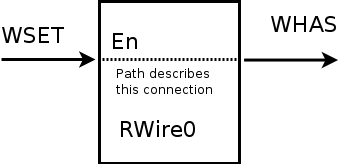
\includegraphics[height= .75 in]{Figures/path}
\caption{Path in the RWire0 Verilog module between WSET and WHAS ports}
\label{pathfig}
\end{center}
\end{figure}

\begin{verbatim}
    import "BVI" RWire0 = 
       module vMkRWire0 (VRWire0);
          ...
          method wset() enable(WSET) ;
          method WHAS whas ;
          schedule whas CF whas ;
          schedule wset SB whas ;
          path (WSET, WHAS) ;
       endmodule: vMkRWire0
\end{verbatim}



\subsection{Interface}
\index{interface@\te{interface} (BVI import statement)}

\gram{interfaceBVIStmt}  { \term{interface} \nterm{typeDefType} \term{;} } \\
\grammore           {\many{ \nterm{interfaceBVIMembDecl} } } \\
\grammore           { \term{endinterface} \opt{ \term{:} \nterm{typeIde} } }

\gram{interfaceBVIMembDecl} {\nterm{methodBVIStmt} }\\
\gramalt           {\nterm{interfaceBVIStmt} \term{;}}


 An interface statement can contain   two types of
statements: method statements and subinterface declarations.
The interface statement in BVI import
is the same as any other interface statement (Section
\ref{sec-interface-decl}) with one difference: the method statements
within the interface  are BVI method statements
(\te{methodBVIStmt} \ref{sec-bvimethod}).  

Example:

\begin{verbatim}
import "BVI" BRAM2 =
module vSyncBRAM2#(Integer memSize, Bool hasOutputRegister,
                   Clock clkA, Reset rstNA, Clock clkB, Reset rstNB
                    ) (BRAM_DUAL_PORT#(addr, data))
   provisos(Bits#(addr, addr_sz),
            Bits#(data, data_sz));
   ...

   interface BRAM_PORT a;
     method put(WEA, (*reg*)ADDRA, (*reg*)DIA) enable(ENA) clocked_by(clkA) reset_by(rstA);
     method DOA read() clocked_by(clkA) reset_by(rstA);
   endinterface: a

   interface BRAM_PORT b;
     method put(WEB, (*reg*)ADDRB, (*reg*)DIB) enable(ENB) clocked_by(clkB) reset_by(rstB);
     method DOB read() clocked_by(clkB) reset_by(rstB);
   endinterface: b
endmodule: vSyncBRAM2
\end{verbatim}

Since a BVI wrapper module can
only provide a single interface (\te{BRAM\_DUAL\_PORT} in this
example), to provide  multiple interfaces you have to create an
interface hierarchy using interface statements.

The  interface hierarchy provided in this example is:
\begin{verbatim}
    interface BRAM_DUAL_PORT#(type addr, type data);
       interface BRAM_PORT#(addr, data) a;
       interface BRAM_PORT#(addr, data) b;
    endinterface: BRAM_DUAL_PORT
\end{verbatim}
where the subinterfaces, \te{a} and \te{b}, are defined as
\te{interface} statements in the body of the \te{import "BVI"} statement.


\subsection{Inout}
\index{inout@\te{inout}(BVI import statement)}

The following statements describe how to pass an \te{inout} port
from a wrapped Verilog module through a BSV module.  These ports
are represented in \BSV{} by the type \te{Inout}.  There are two ways
that an \te{Inout} can appear in \BSV{} modules: as an argument to the
module or as a subinterface of the interface provided by the module.
There are, therefore, two ways to declare an \te{Inout} port in a BVI import:
the statement \te{inout} declares an argument of the current module;
and the statement \te{ifc\_inout} declares a subinterface of the
provided interface.

\gram{inoutBVIStmt} {\term{inout} \nterm{portId}
  \opt{\term{clocked\_by}  \term{(}
   \nterm{clockId} \term{)}}} \\
\grammore {\opt{\term{reset\_by}  \term{(}
   \nterm{resetId} \term{)}} \term{=} \nterm{expression} \term{;}}

The value of \nterm{portId} is the Verilog name of the \te{inout} port
and \nterm{expression} is the name of an argument from the module.

\gram{inoutBVIStmt} {\term{ifc\_inout} \nterm{identifier} \term{(}\nterm{inoutId} \term{)}
  \opt{\term{clocked\_by}  \term{(}
   \nterm{clockId} \term{)}}} \\
\grammore {\opt{\term{reset\_by}  \term{(}
   \nterm{resetId} \term{)}} \term{;}}

Here, the \nterm{identifier} is the name of the subinterface of the provided
interface and \nterm{portId} is, again, the Verilog name of the \te{inout}
port.

The clock and reset associated with the \te{Inout} are assumed to be the
default clock and default reset unless explicitly specified.


% \te{Inout}s are connectable.  When two \te{Inout}s
% are connected using \te{mkConnection}, they must be on the same clock
% and they must be on the same reset.  The clock and reset of the
% \te{inouts} may be different than the clock and reset of the parent
% module of the \te{mkConnection}. 

Example:
\begin{verbatim}
  interface Q;
     interface Inout#(Bit#(13)) q_inout;
     interface Clock c_clock;
  endinterface

  import "BVI" Foo =
  module mkFoo#(Bool b)(Inout#(int) x, Q ifc);   
     default_clock ();
     no_reset;
   
     inout iport = x;

     ifc_inout q_inout(qport);
     output_clock c_clock(clockport);
  endmodule
\end{verbatim}
The wrapped Verilog module is:
\begin{verbatim}
  module Foo (iport, clockport, qport);
     input cccport;
     inout [31:0] iport;
     inout [12:0] qport;
     ...
  endmodule
\end{verbatim}



% ================================================================
\section{Embedding C in a BSV Design}

\index{import ""BDPI""@\te{import ""BDPI""} (keyword)}

This section describes how to declare a BSV function that is provided as
a C  function.  This is used when there are existing C functions
 which the designer would like to include in a
{\BSV} module. Using the \nterm{importBDPI} syntax, the user can
specify that the implementation of a {\BSV} function is provided as a
C function.


\gram{externCImport}   {\term{import} \term{"BDPI"}  \opt{\nterm{identifier}
                       \term{=}} \term{function} \nterm{type}} \\ 
\grammore               {\nterm{identifier}
\term{(} \opt{\nterm{CFuncArgs}} \term{)} \opt{\nterm{provisos}}  \term{;}}\\


\gram{CFuncArgs}      {\nterm{CFuncArg} \many{\term{,} \nterm{CFuncArg}}}\\

\gram{CFuncArg}            {\nterm{type} \opt{\nterm{identifier}}}\\


This defines a function \nterm{identifier} in the BSV source code
which is  implemented by a C function of the same name. A different
link name (C name) can be specified immediately after the
\term{"BDPI"},  using an optional
[\nterm{identifier} = ].   The link
name is  not bound by BSV case-restrictions on identifiers and may
start with  a capital letter.

Example of an import statement where the C name matches the BSV name:
\begin{verbatim}
     // the C function and the BSV function are both named checksum
     import "BDPI" function Bit#(32) checksum (Bit#(n), Bit#(32));     
\end{verbatim}

Example of an import statement where the C name does not match the BSV name:
\begin{verbatim}
     // the C function name is checksum
     // the BSV function name is checksum_raw
     import "BDPI" checksum = function Bit#(32) checksum_raw (Bit#(n), Bit#(32));     
\end{verbatim}

The first \nterm{type} specifies the return type of the function.  The
optional \nterm{CFuncArgs} specify the arguments of the function,
along with an optional identifier to 
name the arguments.

For instance, in the above checksum example, you might want to name the
arguments to indicate that the first argument is the input value and the
second argument is the size of the input value.
\begin{verbatim}
     import "BDPI" function Bit#(32) checksum (Bit#(n) input_val, Bit#(32) input_size);     
\end{verbatim}



\subsection{Argument Types}
The types  for the arguments and return value are BSV types. 
The following table shows the correlation from BSV types to C types.% , for
% 32-bit  versions of BSC. (Since \te{int} is not a fixed size across
% platforms,  these correlations may be different for BSC on other
% platforms.)

\begin{center}
\begin{tabular}{|p {2 in}|p {2 in}|}
\hline
BSV Type&C Type \\
\hline
\hline
\te{String} &	\te{char*} \\
\hline
\te{Bit\#(0)} - \te{Bit\#(8)} &	\te{unsigned char}\\
\hline
\te{Bit\#(9)} - \te{Bit\#(32)}& 	\te{unsigned int}\\
\hline
\te{Bit\#(33)} - \te{Bit\#(64)} & \te{unsigned long long}\\
\hline
\te{Bit\#(65)} - 	&\te{unsigned int*}\\
\hline
\te{Bit\#(n)} &	\te{unsigned int*}\\
\hline
\end{tabular}
\end{center}

The \nterm{importBDPI} syntax provides the ability  to import simple C
functions  that the user may
already have. A C function with an argument of type \te{char} or \te{unsigned
char}  should be imported as a BSV function with an argument of type
\te{Bit\#(8)}.  For \te{int} or \te{unsigned int}, use
\te{Bit\#(32)}. For  \te{long long} or
\te{unsigned  long long}, use \te{Bit\#(64)}. While BSV creates
unsigned  values,
they can be passed to a C function which will treat the value as
signed.  This can be reflected in BSV with \te{Int\#(8)},
\te{Int\#(32)}, \te{Int\#(64)}, etc.

The user may also  import new C functions written to
match a  given BSV function type. For instance, a function on
bit-vectors of  size 17 (that is, \te{Bit\#(17)}) would expect to pass this
value  as the C type \te{unsigned int} and the C function should be aware
that  only the first 17 bits of the value are valid data.

\paragraph{Wide data} Bit vectors of size 65 or greater are passed by reference,
as type  \te{unsigned int*}. This is a pointer to an array of 32-bit words,
where  bit 0 of the BSV vector is bit 0 of the first word in the
array, and  bit 32 of the BSV vector is bit 0 of the second word, 
etc. Note  that we only pass the pointer; no size value is passed to
the C  function. This is because the size is fixed and the C function
could  have the size hardcoded in it. If the function needs the size
as an  additional parameter, then either a C or BSV wrapper is
needed. See  the examples below.

\paragraph{Polymorphic data} As the above table shows, bit vectors of variable
size are  passed by reference, as type \te{unsigned int*}. As with wide
data,  this is a pointer to an array of 32-bit words, where bit 0 of
the BSV  vector is bit 0 of the first word in the array, and bit 32 of
the BSV  vector is bit 0 of the second word, etc. No size value is
passed to  the C function, because the import takes no stance on how
the size  should be communicated. The user will need to handle the
communication of the size, typically by adding an additional argument
to the import  function and using a BSV wrapper to pass the size via
that  argument, as follows:

\begin{verbatim}
     // This function computes a checksum for any size bit-vector
     // The second argument is the size of the input bit-vector
     import "BDPI" checksum = function Bit#(32) checksum_raw (Bit#(n), Bit#(32));

     // This wrapper handles the passing of the size
     function Bit#(32) checksum (Bit#(n) vec);
        return checksum_raw(vec, fromInteger(valueOf(n)));
     endfunction
\end{verbatim}

% For both wide and polymorphic data, the C function receives a pointer
% to the  argument value. The C function should not write to that
% memory. The value to which the C function is pointed will be a copy of
% the simulator state,  so even if the C function does write to this
% memory,  it will not have an effect on the simulation values.

\subsection{Return types}

Imported functions can be value functions, \te{Action} functions, or
\te{ActionValue}  functions. The acceptable return types are the same as
the  acceptable argument types, except that \te{String} is not permitted as
a  return type.

Imported functions with return values correlate to C functions with
return  values, except in the cases of wide and polymorphic data. In
those  cases, where the BSV type correlates to \te{unsigned int*}, 
the simulator  will allocate space for the return result and pass a
pointer to  this memory to the C function. The C function will not be
responsible for allocating memory. When the C function finishes
execution,  the simulator copies the result in that memory to the
simulator  state and frees the memory.
By convention, this special argument is the first argument 
 to the C function.

For example, the following BSV import:
\begin{verbatim}
     import "BDPI" function Bit#(32) f (Bit#(8));
\end{verbatim}
would connect to the following C function:
\begin{verbatim}
     unsigned int f (unsigned char x);
\end{verbatim}
While the following BSV import with wide data:
\begin{verbatim}
     import "BDPI" function Bit#(128) g (Bit#(8));
\end{verbatim}
would connect to the following C function:
\begin{verbatim}
     void g (unsigned int* resultptr, unsigned char x);
\end{verbatim}

% In this case, the simulator knows that the return value of the
% function is  128 bits and allocates that much space. The function \te{g} is
% also  expected to know that the value is 128 bits and to write a
% complete  value into that memory.

\subsection{Implicit pack/unpack}

So far we have only mentioned \te{Bit} and \te{String} types for arguments and
return  values. Other types are allowed as arguments and return
values, as  long as they can be packed into a bit-vector.  These types
include \te{Int}, \te{UInt},
\te{Bool}, and \te{Maybe}, all of which have an 
 instance in the Bits class.  

For example, this is a valid import:
\begin{verbatim}
     import "BDPI" function Bool my_and (Bool, Bool);
\end{verbatim}
Since a \te{Bool} packs to a \te{Bit\#(1)}, it
 would connect to a C function such as the following:
\begin{verbatim} 
     unsigned char
     my_and (unsigned char x, unsigned char y);
\end{verbatim}

In this next example, we have two C functions, \te{signedGT} and
\te{unsignedGT},  both of which  implement a greater-than
function, returning a \te{Bool} indicating whether \te{x} is greater
than \te{y}.
\begin{verbatim}
     import "BDPI" function Bool signedGT (Int#(32) x, Int#(32) y);
     import "BDPI" function Bool unsignedGT (UInt#(32) x, UInt#(32) y);
\end{verbatim}
 Because
the  function \te{signedGT} assumes that the MSB is a sign bit, we use
the  type-system to make sure that we only call that function on
signed  values by specifying  that the function only works on
\te{Int\#(32)}.  Similarly, we can enforce that \te{unsignedGT} is
only called  on unsigned values, by requiring its  arguments
to be of  type \te{UInt\#(32)}.

The C functions would be:
\begin{verbatim}
     unsigned char signedGT (unsigned int x, unsigned int y);
     unsigned char unsignedGT (unsigned int x, unsigned int y);
\end{verbatim}

In both cases, the packed value is of type \te{Bit\#(32)}, and so the
C  function is expected to take the its arguments as \te{unsigned
int}.  The difference is that the \te{signedGT} function will then
treat the  values as signed  values while the \te{unsignedGT} function
will treat them as unsigned values.  Both functions return a
\te{Bool}, which means the C return type is \te{unsigned char}.




Argument and return types to imported functions can also be structs,
enums, and tagged unions. The C function will receive the data in bit
form and must return values in bit form.

\subsection{Other examples}

\paragraph{Shared resources} 
In some situations, several imported functions may share access to a
resource,  such as memory or the file system. If these functions wish
to share  file handles, pointers, or other cookies between each other,
they  will have to pass the data as a bit-vector, such as \te{unsigned
int}/\te{Bit\#(32)}.

\paragraph{When to use Action components} 
If an imported
function has  a side effect or if it matters how many times or in what
order  the function is called (relative to other calls), then the
imported  function should have an \te{Action} component in its BSV type.  That
is, the functions should have a return type of \te{Action} or \te{ActionValue}. 

\paragraph{Removing indirection for polymorphism within a range}
A polymorphic type will always become \te{unsigned int*} in the C,
even if there is a numeric proviso which restricts the size.  
Consider the following import:
\begin{verbatim}
     import "BDPI" function Bit#(n) f(Bit#(n), Bit#(8)) provisos (Add#(n,j,32));
\end{verbatim}
This is a polymorphic vector, so the conversion rules indicate that it
should  appear as \te{unsigned int*} in the C. However, the proviso
indicates  that the value of n can never be greater than 32. 
  To make
the import be a specific size and not a pointer, you could use a
wrapper, as in the example below.
\begin{verbatim}
     import "BDPI" f = function Bit#(32) f_aux(Bit#(32), Bit#(8));

     function Bit#(n) f (Bit#(n) x) provisos (Add#(n,j,32));
        return f_aux(extend(x), fromInteger(valueOf(n)));
     endfunction
\end{verbatim}


% ================================================================

\bibliography{lang}
\bibliographystyle{alpha}

% The following two commands are a work-around for some bug
% seemingly introduced by the fancyhdr package.  Without this,
% the entries on the last page of the bibliography are spread
% vertically across the page, i.e., the linespacing is
% screwed up.  This work-around seems to fix it.

\vfill

\hm

% ================================================================

\pagebreak

\appendix

% ================================================================

\section{Keywords}

\label{sec-keywords}

In general, keywords do not use uppercase letters (the only exception
is the keyword \texttt{valueOf}). The following are the keywords in
{\BSV} (and so they cannot be used as identifiers).

% The following input file is produced automatically by extracting all
% the keywords from the grammar productions throughout this document.

\input{keywords.tex}

% The following two commands are a work-around for some bug
% seemingly introduced by the fancyhdr package.  Without this,
% the entries on the last page of the table of are spread
% vertically across the page, i.e., the linespacing is
% screwed up.  This work-around seems to fix it.

\vfill

\hm

\pagebreak

The following are keywords in SystemVerilog (which includes all the
keywords in Verilog).  Although most of them are not used in {\BSV},
for compatibility reasons they are not allowed as identifiers in
{\BSV} either.

\begin{minipage}[t]{14em}\small
 \begin{verbatim}
  alias
  always
  always_comb
  always_ff
  always_latch
  and
  assert
  assert_strobe
  assign
  assume
  automatic
  before
  begin   end
  bind
  bins
  binsof
  bit
  break
  buf
  bufif0
  bufif1
  byte
  case    endcase
  casex
  casez
  cell
  chandle
  class       endclass
  clocking    endclocking
  cmos
  config      endconfig
  const
  constraint
  context
  continue
  cover
  covergroup  endgroup
  coverpoint
  cross
  deassign
  default
  defparam
  design
  disable
  dist
  do
  edge
  else
  enum
  event
 \end{verbatim}
\end{minipage}
\begin{minipage}[t]{14em}\small
 \begin{verbatim}
  expect
  export
  extends
  extern
  final
  first_match
  for
  force
  foreach
  forever
  fork
  forkjoin
  function    endfunction
  generate    endgenerate
  genvar
  highz0
  highz1
  if
  iff
  ifnone
  ignore_bins
  illegal_bins
  import
  incdir
  include
  initial
  inout
  input
  inside
  instance
  int
  integer
  interface   endinterface
  intersect
  join
  join_any
  join_none
  large
  liblist
  library
  local
  localparam
  logic
  longint
  macromodule
  matches
  medium
  modport
  module       endmodule
  nand
 \end{verbatim}
\end{minipage}
\begin{minipage}[t]{14em}\small
 \begin{verbatim}
  negedge
  new
  nmos
  nor
  noshowcancelled
  not
  notif0
  notif1
  null
  or
  output
  package      endpackage
  packed
  parameter
  pmos
  posedge
  primitive    endprimitive
  priority
  program      endprogram
  property     endproperty
  protected
  pull0
  pull1
  pulldown
  pullup
  pulsestyle_onevent
  pulsestyle_ondetect
  pure
  rand
  randc
  randcase
  randsequence
  rcmos
  real
  realtime
  ref
  reg
  release
  repeat
  return
  rnmos
  rpmos
  rtran
  rtranif0
  rtranif1
  scalared
  sequence     endsequence
  shortint
  shortreal
  showcancelled
 \end{verbatim}
\end{minipage}

\begin{minipage}[t]{14em}\small
 \begin{verbatim}
  signed
  small
  solve
  specify      endspecify
  specparam
  static
  string
  strong0
  strong1
  struct
  super
  supply0
  supply1
  table        endtable
  tagged
  task         endtask
  this
  throughout
 \end{verbatim}
\end{minipage}
\begin{minipage}[t]{14em}\small
 \begin{verbatim}
  time
  timeprecision
  timeunit
  tran
  tranif0
  tranif1
  tri
  tri0
  tri1
  triand
  trior
  trireg
  type
  typedef
  union
  unique
  unsigned
  use
 \end{verbatim}
\end{minipage}
\begin{minipage}[t]{14em}\small
 \begin{verbatim}
  var
  vectored
  virtual
  void
  wait
  wait_order
  wand
  weak0
  weak1
  while
  wildcard
  wire
  with
  within
  wor
  xnor
  xor
 \end{verbatim}
\end{minipage}

% ================================================================

\pagebreak

% ================================================================

\section{A Brief History of {\BH} (Bluespec Haskell/Classic) and {\BSV} (Bluespec SystemVerilog)}

\label{sec-history}

The original research on using \emph{rules} to specify hardware
behavior, and of compiling rules into synthesizable Verilog was
conducted by James Hoe for his Ph.D. thesis \cite{jhoe} under the
supervision of Prof. Arvind at MIT in the late 1990s.

In 2000, activity moved to Sandburst Corp., a fabless semiconductor
startup company based in Massachusetts, producing enterprise-class and
metropolitan-class network router chips.  The first Bluespec language
and compiler were designed at Sandburst by Lennart Augustsson, with
the assistance of several others including Jacob Schwartz, Mieszko
Lis, Joe Stoy, Arvind and Rishiyur Nikhil.  The language was very much
Haskell-influenced in its syntax, in its type system, and in its
static elaboration semantics.  The compiler itself was written in
Haskell.  During this period, the language was used only in-house,
principally for hardware-models of Sandburst's chip architecture.

In 2003, a separate company, Bluespec, Inc., also in Massachusetts,
was spun out from Sandburst Corp. to focus on the Bluespec language
and compiler as its central product, targeted at digital design
engineers worldwide.  Because of the target audence's deep familiarity
with Hardware Design Languages (principally Verilog and VHDL), and
complete unfamiliarity with Haskell, the syntax of the Bluespec
language was completely redesigned to be as similar as possible to
SystemVerilog, which was just then being defined as an industry
standard.  Members of Bluespec, Inc. joined the IEEE SystemVerilog
standardization effort, for closer alignment (the ``tagged unions''
and ``pattern-matching'' constructs in the SystemVerilog standard were
a Bluespec contribution, inspired directly by Haskell).

The original Haskell-like syntax (at Sandburst Corp.) and the
subsequent SystemVerilog-like syntax (at Bluespec, Inc.) are merely
two different syntaxes for the same language, with the same semantics.
They are simply two alternative parsing front-ends for the common
{\bsc} compiler.  The original language is called ``Bluespec Classic''
or {\BH} (for ``Bluespec Haskell'') and the subsequent language is
called {\BSV} (for ``Bluespec SystemVerilog'').  Both syntaxes
continue to be accepted by {\bsc}, and a single system can mix and
match packages, some written in BH and some written in BSV.  Almost
all designs from 2005 onwards were done in BSV (with one major
exception done in BH), but since open-sourcing in 2020, BH is once
again seeing increased use.

From about 2005 to 2020, {\bsc} was a product of Bluespec, Inc.,
licensed commercially to companies and non-academic institutions, with
free licenses to universities for teaching and research.  During this
time, BSV was used for production ASIC designs in several top-ten
semiconductor companies, a network devices company, and a major
Internet company, and for high-level architectural modeling in a few
top-ten computer companies.  Bluespec, Inc. itself does all its RISC-V
CPU and system designs in BSV (many open-sourced on GitHub).  Amongst
universities, MIT (USA), University of Cambridge (UK) and IIT Madras
(India) have been and continue to be leading users.

Bluespec, Inc. has always considered the language to be fully open
(i.e., anyone can freely build their own language implementation); the
only proprietary artefact was Bluespec, Inc.'s own implementation, the
{\bsc} compiler.  In 2010, at an IEEE SystemVerilog Standards
Committee planning meeting, Bluespec, Inc. offered to donate the whole
of the BSV language definition for incorporation into the
SystemVerilog standard, but this offer did not garner enough votes for
acceptance.

In 2020, Bluespec, Inc. released the {\bsc} compiler (and related
proprietary artefacts: Bluesim, Bluespec Development Workstation,
etc.) in fully open-source form.  All the source codes etc. are now
hosted in open GitHub repositories, and there are now many
contributors from diverse locations worldwide.

% ================================================================

% The following is about Standard Prelude and Azure Foundation
% Libraries and has been moved to a separate "Libraries Reference
% Guide" document

% \input{lang_lib_sections}

% ================================================================

\clearpage
\phantomsection
\addcontentsline{toc}{section}{Index}
\printindex

\end{document}
